\documentclass{memoir}
\usepackage[dvipsnames]{xcolor} % Required for specifying custom colors
\usepackage[showframe=false]{geometry} % Required for adjusting page dimensions and margins
\usepackage[colorlinks=true, linkcolor=blue, citecolor=blue, urlcolor=blue]{hyperref}
% Packages for custom shapes and boxes
\usepackage{tikz} % Required for drawing custom shapes
\usepackage[framemethod=TikZ]{mdframed} % Required for creating the theorem, definition, exercise and corollary boxes
% \newcounter{theo}[section]\setcounter{theo}{0}

% THEOREM BOXES
\newcounter{theo}[section]\setcounter{theo}{0}
\renewcommand{\thetheo}{\arabic{section}.\arabic{theo}}

\newenvironment{theo}[2][]{%
    \refstepcounter{theo}

    \ifstrempty{#1}%
    % if condition (without title)
    {\mdfsetup{%
            frametitle={%
                    \tikz[baseline=(current bounding box.east),outer sep=0pt]
                    \node[anchor=east,rectangle,fill=black,text=white]
                    {\strut Theorem~\thetheo};}
        }%
        % else condition (with title)
    }{\mdfsetup{%
            frametitle={%
                    \tikz[baseline=(current bounding box.east),outer sep=0pt]
                    \node[anchor=east,rectangle,fill=black,text=white]
                    {\strut Theorem~\thetheo:~#1};}%
        }%
    }%
    % Both conditions
    \mdfsetup{%
        innertopmargin=6pt,innerbottommargin=12pt,linecolor=black,%
        linewidth=2pt,topline=true,%
        frametitleaboveskip=\dimexpr-\ht\strutbox\relax%
    }

    \begin{mdframed}[]\relax}{
    \end{mdframed}}

% DEFINITION BOXES
\newcounter{Def}[section]\setcounter{Def}{0}
\renewcommand{\theDef}{\arabic{section}.\arabic{Def}}

\newenvironment{Def}[2][]{%
    \refstepcounter{Def}

    \ifstrempty{#1}%
    % if condition (without title)
    {\mdfsetup{%
            frametitle={%
                    \tikz[baseline=(current bounding box.east),outer sep=0pt]
                    \node[anchor=east,rectangle,fill=black,text=white]
                    {\strut Definition~\theDef};}
        }%
        % else condition (with title)
    }{\mdfsetup{%
            frametitle={%
                    \tikz[baseline=(current bounding box.east),outer sep=0pt]
                    \node[anchor=east,rectangle,fill=black,text=white]
                    {\strut Definition~\theDef:~#1};}%
        }%
    }%
    % Both conditions
    \mdfsetup{%
        innertopmargin=6pt,
        innerbottommargin=12pt,
        linecolor=black,%
        linewidth=2pt,topline=true,%
        frametitleaboveskip=\dimexpr-\ht\strutbox\relax%
    }

    \begin{mdframed}[]\relax}{%
    \end{mdframed}}


% TIP BOXES
\newcounter{Tip}[section]\setcounter{Tip}{0}
\renewcommand{\theTip}{\arabic{section}.\arabic{Tip}}

\newenvironment{Tip}{%
    \refstepcounter{Tip}
    \mdfsetup{%
        backgroundcolor=OliveGreen!10,
        innertopmargin=12pt,
        innerbottommargin=12pt,
        linecolor=black,
        linewidth=0pt,
        topline=false,
        frametitleaboveskip=\dimexpr-\ht\strutbox\relax
    }
    \begin{mdframed}[]\relax
        \textbf{Tip:}
        }{%
    \end{mdframed}
}

% GREEN BOXES
\newenvironment{greenbox}{%
    \mdfsetup{%
        backgroundcolor=OliveGreen!10,
        innertopmargin=12pt,
        innerbottommargin=12pt,
        linecolor=black,
        linewidth=0pt,
        topline=false,
        frametitleaboveskip=\dimexpr-\ht\strutbox\relax
    }
    \begin{mdframed}[]\relax

        }{%
    \end{mdframed}
}

% GRAY BOXES
\newenvironment{graybox}{%
    \mdfsetup{%
        backgroundcolor=black!10,
        innertopmargin=12pt,
        innerbottommargin=12pt,
        linecolor=black,
        linewidth=0pt,
        topline=false,
        frametitleaboveskip=\dimexpr-\ht\strutbox\relax
    }
    \begin{mdframed}[]\relax

        }{%
    \end{mdframed}
}

% NOTE BOXES
\newcounter{Note}[section]\setcounter{Note}{0}
\renewcommand{\theNote}{\arabic{section}.\arabic{Note}}

\newenvironment{Note}{%
    \refstepcounter{Note}
    \mdfsetup{%
        backgroundcolor=black!10,
        innertopmargin=10pt,
        innerbottommargin=8pt,
        linecolor=black,
        linewidth=0pt,
        topline=false,
        frametitleaboveskip=\dimexpr-\ht\strutbox\relax
    }
    \begin{mdframed}[]\relax
        }{%
    \end{mdframed}
}

% GENERIC BOXES

\newenvironment{gbox}{%
    \mdfsetup{%
        backgroundcolor=white,
        innertopmargin=12pt,
        innerbottommargin=6pt,
        linecolor=black,
        linewidth=1pt,
        topline=true,
        frametitleaboveskip=\dimexpr-\ht\strutbox\relax
    }
    \begin{mdframed}[]\relax
        % Your content goes here
        }{%
    \end{mdframed}
}

% PROOF BOXES

% \newcounter{theo}[section]\setcounter{theo}{0}

% PROOF BOXES

\newcounter{Proof}[section]\setcounter{Proof}{0}
\renewcommand{\theProof}{\arabic{section}.\arabic{Proof}}

\newenvironment{Proof}[1][]{%
    \refstepcounter{Proof}

    \ifstrempty{#1}%
    % if condition (without title)
    {\mdfsetup{%
            frametitle={%
                    \tikz[baseline=(current bounding box.east),outer sep=0pt]
                    \node[anchor=east,rectangle,fill=white,text=black]
                    {\strut Proof~\theProof};}
        }%
        % else condition (with title)
    }{\mdfsetup{%
            frametitle={%
                    \tikz[baseline=(current bounding box.east),outer sep=0pt]
                    \node[anchor=east,rectangle,fill=white,text=black]
                    {\strut Proof~\theProof:~#1};}%
        }%
    }%
    % Both conditions
    \mdfsetup{%
        innertopmargin=6pt,
        innerbottommargin=12pt,
        linecolor=black,%
        linewidth=1pt,topline=true,%
        frametitleaboveskip=\dimexpr-\ht\strutbox\relax%
    }

    \begin{mdframed}[]\relax}{
        \hfill$\blacksquare$
    \end{mdframed}
}

% EXAMPLE BOXES

\newcounter{Example}[section]\setcounter{Example}{0}
\renewcommand{\theExample}{\arabic{section}.\arabic{Example}}

\newenvironment{Example}[1][]{%
    \refstepcounter{Example}

    \ifstrempty{#1}%
    % if condition (without title)
    {\mdfsetup{%
            frametitle={%
                    \tikz[baseline=(current bounding box.east),outer sep=0pt]
                    \node[anchor=east,rectangle,fill=white,text=black]
                    {\strut Example~\theExample};}
        }%
        % else condition (with title)
    }{\mdfsetup{%
            frametitle={%
                    \tikz[baseline=(current bounding box.east),outer sep=0pt]
                    \node[anchor=east,rectangle,fill=white,text=black]
                    {\strut Example~\theExample:~#1};}%
        }%
    }%
    % Both conditions
    \mdfsetup{%
        innertopmargin=6pt,
        innerbottommargin=12pt,
        linecolor=black,%
        linewidth=1pt,topline=true,%
        frametitleaboveskip=\dimexpr-\ht\strutbox\relax%
    }

    \begin{mdframed}[]\relax}{
        \hfill$\blacksquare$
    \end{mdframed}
}

% Function Counter
\newcounter{Func}[section]
\renewcommand{\theFunc}{\arabic{section}.\arabic{Func}}

% Function Environment
\newenvironment{Func}[1][]{
    \refstepcounter{Func}
    \ifstrempty{#1}% 
    {% If no title is provided
        \mdfsetup{
            frametitle={
                \tikz[baseline=(current bounding box.east),outer sep=0pt]
                \node[anchor=east,rectangle,fill=black,text=white]
                {\strut Function~\theFunc};}
        }
    }{% If a title is provided
        \mdfsetup{
            frametitle={
                \tikz[baseline=(current bounding box.east),outer sep=0pt]
                \node[anchor=east,rectangle,fill=black,text=white]
                {\strut Function~\theFunc:~#1};}
        }
    }
    % Common settings for both cases
    \mdfsetup{
        innertopmargin=10pt,
        innerbottommargin=10pt,
        skipabove=\baselineskip,
        skipbelow=\baselineskip,
        linecolor=black,
        linewidth=1pt,
        topline=true,
        frametitleaboveskip=\dimexpr-\ht\strutbox\relax,
        frametitlealignment=\raggedright
    }
    \begin{mdframed}
}{
    \end{mdframed}
}

 % This file contains the code for the boxes

% Packages for math symbols and images
\usepackage{amssymb} % Math symbols such as \mathbb
\usepackage{amsmath} % Required for \begin{align}...\end{align}
\DeclareMathOperator{\lcm}{lcm}
\usepackage{mathtools}
\DeclarePairedDelimiter\ceil{\lceil}{\rceil}
\DeclarePairedDelimiter\floor{\lfloor}{\rfloor}
\usepackage{graphicx} % Required for including images

% Tables
\usepackage{multirow} % Required for creating multirow cells in tables
\usepackage{array} % Required for creating tables
\usepackage{colortbl} % Add this line to import the colortbl package
\setlength{\tabcolsep}{18pt} % Default value: 6pt
\renewcommand{\arraystretch}{1.5} % Default value: 1
\usepackage{changepage} % Required for adjusting the width of the table


% Package for customizing captions
\usepackage{caption}  % Required for customizing captions

\usepackage{setspace} % Required for adjusting line spacing
\usepackage{etoolbox} % For \ifstrempty

\usepackage{subcaption} % for subfigures

\usepackage[linesnumbered, noend]{algorithm2e}
\usepackage{algpseudocode}
\usepackage{makecell} % for line break in table cell

\usepackage{longdivision}% Package for long division algorithm

% commands

% Tikz
% \tikzset{
%     pics/machine/.style={
%             code={
%                     \coordinate (-in) at ({-0.5*\pgfkeysvalueof{/tikz/machine/width}},0);
%                     \coordinate (-out) at ({0.5*\pgfkeysvalueof{/tikz/machine/width}},0);
%                     \coordinate (-north) at (0,{0.5*\pgfkeysvalueof{/tikz/machine/height}});
%                     \coordinate (-south) at (0,{-0.5*\pgfkeysvalueof{/tikz/machine/height}});
%                     \path[/tikz/machine/filling]
%                     ([shift={(-0.75em,0.5em)}]-in)
%                     -- ([shift={(0,0.25em)}]-in)
%                     -- ([shift={(0,-5pt)}]-north -| -in)
%                     arc[start angle=180, end angle=90, radius=5pt]
%                     -- ([shift={(-5pt,0)}]-north -| -out)
%                     arc[start angle=90, end angle=0, radius=5pt]
%                     -- ([shift={(0,0.25em)}]-out)
%                     -- ([shift={(0.75em,0.5em)}]-out)
%                     -- ([shift={(0.75em,-0.5em)}]-out)
%                     -- ([shift={(0,-0.25em)}]-out)
%                     -- ([shift={(0,5pt)}]-south -| -out)
%                     arc[start angle=360, end angle=270, radius=5pt]
%                     -- ([shift={(5pt,0)}]-south -| -in)
%                     arc[start angle=270, end angle=180, radius=5pt]
%                     -- ([shift={(0,-0.25em)}]-in)
%                     -- ([shift={(-0.75em,-0.5em)}]-in)
%                     -- cycle;
%                     \draw[/tikz/machine/border]
%                     ([shift={(-0.75em,0.5em)}]-in)
%                     -- ([shift={(0,0.25em)}]-in)
%                     -- ([shift={(0,-5pt)}]-north -| -in)
%                     arc[start angle=180, end angle=90, radius=5pt]
%                     -- ([shift={(-5pt,0)}]-north -| -out)
%                     arc[start angle=90, end angle=0, radius=5pt]
%                     -- ([shift={(0,0.25em)}]-out)
%                     -- ([shift={(0.75em,0.5em)}]-out);
%                     \draw[/tikz/machine/border]
%                     ([shift={(0.75em,-0.5em)}]-out)
%                     -- ([shift={(0,-0.25em)}]-out)
%                     -- ([shift={(0,5pt)}]-south -| -out)
%                     arc[start angle=360, end angle=270, radius=5pt]
%                     -- ([shift={(5pt,0)}]-south -| -in)
%                     arc[start angle=270, end angle=180, radius=5pt]
%                     -- ([shift={(0,-0.25em)}]-in)
%                     -- ([shift={(-0.75em,-0.5em)}]-in);
%                     \node (-node) at (0,0) {#1};
%                 }
%         },
%     machine/width/.initial={10.5em},
%     machine/height/.initial={5em},
%     machine/filling/.style={
%             left color=cyan!50!OliveGreen!25,
%             right color=cyan!50!OliveGreen!25,
%             middle color=cyan!50!OliveGreen!10
%         },
%     machine/border/.style={
%             OliveGreen!50!cyan
%         }
% }

% Color Text
\definecolor{BlueText}{RGB}{0,51,204}
\newcommand{\bt}[1]{\textcolor{BlueText}{#1}}

\newcommand{\Div}{%
    \par\noindent\hrulefill\par
}

\renewcommand{\clearforchapter}{ \newpage}

\makeatletter
\NewCommandCopy\@@pmod\pmod
\DeclareRobustCommand{\pmod}{\@ifstar\@pmods\@@pmod}
\def\@pmods#1{\mkern4mu({\operator@font mod}\mkern 6mu#1)}
\makeatother



\newcolumntype{g}{>{\columncolor{OliveGreen!10}}c}

\newcommand{\qres}{(\mathbb{Z}_p^*)^2}
\newcommand{\ires}{(\mathbb{Z}_n^*)^2}
\newcommand{\pres}{\mathbb{Z}_p^*}
\newcommand{\peres}{\mathbb{Z}_{p^{e}}^*}
\newcommand{\gres}{\mathbb{Z}_n}
\newcommand{\Z}{\mathbb{Z}}


\algnewcommand\algorithmicforeach{\textbf{for each}}
\algdef{S}[FOR]{ForEach}[1]{\algorithmicforeach\ #1\ \algorithmicdo}

\newcommand*{\carry}[1][1]{\overset{#1}}
\newcolumntype{B}[1]{r*{#1}{@{\,}r}}

\title{Introduction to Information Security}
\author{Christian J. Rudder}
\date{November 2024}

\chapterstyle{dash} % Chatper style
\setlength{\beforechapskip}{-1em} % Adjusts space before the chapter heading


\begin{document}

\maketitle
\setcounter{tocdepth}{2}

\tableofcontents

% Intentionally left blank
\newpage
\thispagestyle{empty}
\mbox{}
\vfill
\begin{center}
    \textit{This page is left intentionally blank.}
\end{center}
\vfill
\newpage
\thispagestyle{empty}
\mbox{}
\vfill
\begin{center}
    \Large{Big thanks to \textbf{Professor Sharon Goldberg}}\\
    \normalsize 
    for teaching CS357 (Introduction to Information Security)\\
    at Boston University.\\

    \vspace{2em}
    \textit{The following five sections are pre-requisites from Concise Work Section Modules \cite{concise_works_modules}.}\\
    \textbf{Available at:} \url{https://github.com/Concise-Works/sect-modules}.\\
    These are not needed, but are recommended for a better understanding of the material.\\
    
    
\end{center}
\vfill

% \chapter{Prerquesites}
% 

\section{Asymptotic Notation}

Asymptotic analysis is a method for describing the limiting behavior of functions as inputs grow infinitely.

\begin{Def}[Asymptotic]
    
    Let \(f(n)\) and \(g(n)\) be two functions. As \(n\) grows, if \(f(n)\) grows closer to \(g(n)\) never reaching, we say that \underline{``$f(n)$ is \textbf{asymptotic} to \(g(n)\).''}\\
    
    \noindent
    We call the point where \(f(n)\) starts behaving similarly to \(g(n)\) the \underline{\textbf{threshold} \(n_0\).} After this point $n_0$, \(f(n)\) follows the same general path as \(g(n)\).
\end{Def}

\begin{Def}[Big-O: (Upper Bound)]

    Let $f$ and $g$ be functions. $f(n)$ our function of interest, and $g(n)$
    our function of comparison.\\

    \noindent
    Then we say $f(n)=O(g(n))$, ``$f(n)$ \textbf{is big-O of} $g(n)$,'' if $f(n)$ 
    grows no faster than $g(n)$, up to a constant factor.
    Let $n_0$ be our asymptotic threshold. Then, for all $n\geq n_0$,
    \large
    \[0\leq f(n) \leq c\cdot g(n)\]
    \normalsize
    
    \noindent
    Represented as the ratio $\dfrac{f(n)}{g(n)}\leq c$ for all $n\geq n_0$. Analytically we write,
    \Large
    \[\lim_{n\to\infty}\dfrac{f(n)}{g(n)}< \infty\]
    \normalsize
    \noindent
    Meaning, as we chase infinity, our numerator grows slower than the denominator, bounded, never reaching infinity. 
\end{Def}

\newpage

\noindent
\textbf{Examples:}
\begin{enumerate}
    \item[(i.)] $3n^2+2n+1=O(n^2)$
    \item[(ii.)] $n^{100}=O(2^n)$
    \item[(iii.)] $\log n=O(\sqrt{n})$ 
\end{enumerate}

\begin{Proof}[$\log n = O(\sqrt{n})$]
We setup our ratio:
\[\lim_{n\to\infty}\dfrac{\log n}{\sqrt{n}}\]
\noindent
Since $\log n$ and $\sqrt{n}$ grow infinitely without bound, they are of indeterminate form $\frac{\infty}{\infty}$. We apply L'Hopital's Rule, which states
that taking derivatives of the numerator and denominator will yield an evaluateable limit:
\Large
\[\lim_{n\to\infty}\dfrac{\log n}{\sqrt{n}}=\lim_{n\to\infty}\dfrac{\frac{d}{dn}\log n}{\frac{d}{dn}\sqrt{n}}\]
\normalsize
\noindent
Yielding derivatives, $\log n = \frac{1}{n}$ and $\sqrt{n}=\frac{1}{2\sqrt{n}}$. We substitute these back into our limit:
\Large
\[\lim_{n\to\infty}\dfrac{\frac{1}{n}}{\frac{1}{2\sqrt{n}}}=\lim_{n\to\infty}\dfrac{2\sqrt{n}}{n}=\lim_{n\to\infty}\dfrac{2}{\sqrt{n}}=0\]
\normalsize
\noindent
Our limit approaches 0, as we have a constant factor in the numerator, and a growing denominator. Thus, $\log n = O(\sqrt{n})$, as $0<\infty$.
\end{Proof}

\begin{Def}[Big-$\Omega$: (Lower Bound)]

    The symbol $\Omega$ reads ``Omega.'' Let $f$ and $g$ be functions. Then 
    $f(n)=\Omega(g(n))$ if $f(n)$ grows no slower than $g(n)$, up to a constant factor. I.e.,
    lower bounded by $g(n)$. Let $n_0$ be our asymptotic threshold. Then, for all $n\geq n_0$,
    \large
    \[0\leq c\cdot g(n) \leq f(n)\]
    \[0<\lim_{n\to\infty}\dfrac{f(n)}{g(n)}\]
    \normalsize
    \noindent
    Meaning, as we chase infinity, our numerator grows faster than the denominator, approaching 0 asymptotically.
\end{Def}

\noindent
\textbf{Examples:} $n!=\Omega(2^n)$; $\dfrac{n}{100}= \Omega(n)$; $n^{3/2}= \Omega(\sqrt{n})$; $\sqrt{n} = \Omega(\log n)$

\newpage

\begin{Def}[Big $\Theta$: (Tight Bound)]

    The symbol $\Theta$ reads ``Theta.'' Let $f$ and $g$ be functions. Then $f(n)=\Theta(g(n))$ if $f(n)$ grows at the same rate as $g(n)$, up to a constant factor. I.e., $f(n)$ is both upper and lower bounded by $g(n)$. Let $n_0$ be our asymptotic threshold, and $c_1>0,c_2>0$ be some constants. Then, for all $n\geq n_0$,
    \large
    \[0\leq c_1\cdot g(n) \leq f(n) \leq c_2\cdot g(n)\]
    \[0<\lim_{n\to\infty}\dfrac{f(n)}{g(n)}<\infty\]
    \normalsize
    \noindent
    Meaning, as we chase infinity, our numerator grows at the same rate as the denominator.
\end{Def}
\noindent
\textbf{Examples:} $n^2=\Theta(n^2)$; $2n^3+2n=\Theta(n^3)$; $\log n+\sqrt{n}=\Theta(\sqrt{n})$.
\begin{Def}[Little $o$: (Strict Upper Bound)]

    The symbol $o$ reads ``little-o.'' Let $f$ and $g$ be functions. Then $f(n)=o(g(n))$ if $f(n)$ grows strictly slower than $g(n)$, meaning $f(n)$ becomes insignificant compared to $g(n)$ as $n$ grows large. Let $n_0$ be our asymptotic threshold. Then, for all $n\geq n_0$,
    \large
    \[0\leq f(n) < c \cdot g(n)\]
    \[\lim_{n\to\infty}\dfrac{f(n)}{g(n)}=0\]
    \normalsize
    \noindent
    Meaning, as we chase infinity, the ratio of $f(n)$ to $g(n)$ shrinks to zero.
\end{Def}
\noindent
\textbf{Examples:} $n=\!o(n^2)$; $\log n=\!o(n)$; $n^{0.5}=\!o(n)$.
\begin{Def}[Little $\omega$: (Strict Lower Bound)]

    The symbol $\omega$ reads ``little-omega.'' Let $f$ and $g$ be functions. Then $f(n)=\omega(g(n))$ if $f(n)$ grows strictly faster than $g(n)$, meaning $g(n)$ becomes insignificant compared to $f(n)$ as $n$ grows large. Let $n_0$ be our asymptotic threshold. Then, for all $n\geq n_0$,
    \large
    \[0\leq c \cdot g(n) < f(n)\]
    \[\lim_{n\to\infty}\dfrac{g(n)}{f(n)}=0\]
    \normalsize
    \noindent
    Meaning, as we chase infinity, the ratio of $g(n)$ to $f(n)$ shrinks to zero.
\end{Def}
\noindent
\textbf{Examples:} $n^2=\omega(n)$; $n=\omega(\log n)$.

\newpage 

\begin{Def}[Asymptotic Equality (\( \sim \))]

    The symbol \( \sim \) reads ``asymptotic equality.'' Let $f$ and $g$ be functions. Then $f(n) \sim g(n)$ if, as $n \to \infty$, the ratio of $f(n)$ to $g(n)$ approaches 1. I.e., the two functions grow at the same rate asymptotically. Formally,
    \large
    \[\lim_{n\to\infty}\dfrac{f(n)}{g(n)}=1\]
    \normalsize
    \noindent
    Meaning, as $n$ grows large, the two functions become approximately equal.
\end{Def}
\noindent
\textbf{Examples:} $n + 100 \sim n, \quad \log(n^2) \sim 2\log n.$


\begin{Tip}
    To review:
    \begin{itemize}
        \item \textbf{Big-$O$:} $f(n)$ < $g(n)$ (Upper Bound); $f(n)$ grows no faster than $g(n)$.
        \item \textbf{Big-$\Omega$:} $f(n)$ > $g(n)$ (Lower Bound); $f(n)$ grows no slower than $g(n)$.
        \item \textbf{Big-$\Theta$:} $f(n)$ = $g(n)$ (Tight Bound); $f(n)$ grows at the same rate as $g(n)$.
        \item \textbf{Little-$o$:} $f(n)$ < $g(n)$ (Strict Upper Bound); $f(n)$ grows strictly slower than $g(n)$.
        \item \textbf{Little-$\omega$:} $f(n)$ > $g(n)$ (Strict Lower Bound); $f(n)$ grows strictly faster than $g(n)$.
        \item \textbf{Asymptotic Equality:} $f(n)$ $\sim$ $g(n)$; $f(n)$ grows at the same rate as $g(n)$.
    \end{itemize}
\end{Tip}

\begin{theo}[Types of Asymptotic Behavior]

    The following are common relationships between different types of functions and their asymptotic growth rates:

    \begin{itemize}
        \item \textbf{Polynomials.} Let $f(n) = a_0 + a_1 n + \dots + a_d n^d$ with $a_d > 0$. Then, \underline{$f(n)$ is $\Theta(n^d)$.}\\
        E.e., $3n^2+2n+1$ is $\Theta(n^2)$.
        
        \item \textbf{Logarithms.} \underline{$\Theta(\log_a n)$ is $\Theta(\log_b n)$} for any constants $a, b > 0$. That is, logarithmic functions in different bases have the same growth rate.\\
        E.g., $\log_2 n$ is $\Theta(\log_3 n)$.
        
        \item \textbf{Logarithms and Polynomials.} For every $d > 0$, \underline{$\log n$ is $O(n^d)$.} This indicates that logarithms grow slower than any polynomial.\\
        E.g., $\log n$ is $O(n^2)$.
        
        \item \textbf{Exponentials and Polynomials.} For every $r > 1$ and every $d > 0$, \underline{$n^d$ is $O(r^n)$.} This means that exponentials grow faster than any polynomial.\\
        E.e., $n^2$ is $O(2^n)$.
    \end{itemize}
\end{theo}

\newpage 
\section{Evaluating Algorithms}
\noindent
When analyzing algorithms, we are interested in two primary factors: time and space complexity.

\begin{Def}[Time Complexity]
    
        The \textbf{time complexity} of an algorithm is the amount of time it takes to run as a function of the input size. We use asymptotic notation to describe the time complexity of an algorithm.
\end{Def}

\begin{Def}[Space Complexity]
    
        The \textbf{space complexity} of an algorithm is the amount of memory it uses to store inputs and subsequent variables during the algorithm's execution. We use asymptotic notation to describe the space complexity of an algorithm.
\end{Def}
\noindent
Below is an example of a function and its time and space complexity analysis.

\begin{Func}[Arithmetic Series - \texttt{Fun1($A$)}]
    Computes a result based on a length-$n$ array of integers:

    \vspace{.5em}
    \noindent
    \textbf{Input: } A length-$n$ array of integers.\\
    \textbf{Output: } An integer $p$ computed from the array elements.\\
    \begin{algorithm}[H]
        \SetAlgoLined
        
        \vspace{.5em}
        \SetKwProg{Fn}{Function}{:}{\KwRet{$p$}}
        \Fn{\texttt{Fun1($A$)}}{
            $p \gets 0$\;
            \For{$i \gets 1$ \KwTo $n-1$}{
                \For{$j \gets i+1$ \KwTo $n$}{
                    $p \gets p + A[i] \cdot A[j]$\;
                }
            }
        }
    \end{algorithm}

    \noindent
    \textbf{Time Complexity:} For $f(n):=$ \texttt{Fun1($A$)}, $f(n)=\frac{n^2}{2}=O(n^2)$. This is because the function has a nested loop structure, where the inner for-loop runs $n-i$ times, and the outer for-loop runs $n-1$ times. Thus, the total number of iterations is $\sum_{i=1}^{n-1}n-i=\frac{n^2}{2}$.\\

    \noindent
    \textbf{Space Complexity:} We yield $O(n)$ for storing an array of length $n$. The variable $p$ is $O(1)$ (constant), as it is a single integer. Hence, $f(n)=n+1=O(n)$.
    \end{Func}   

    \noindent
    \textbf{Additional Example:} Let $f(n,m) = n^2m + m^3 + nm^3$. Then, $f(n,m)=O(n^2m+m^3)$. This is because both $n$ and $m$ must be accounted for. Our largest $n$ term is $n^2m$, and our largest $m$ term is $m^3$ both dominate the expression. Thus, $f(n,m)=O(n^2m+m^3)$.




% % \vspace{-2em}
\section{Inductive Analysis}

Recursion employs techniques of repeatedly shrinking the problem to solve its smaller halves. Often found in sorting problems, processing trees, and
geometric problems.

\begin{theo}[MergeSort]
    
    Given an array $A$ of size $n$, we sort via the following:
    \begin{enumerate}
        \item [(i.)] Recursively: Split the array into two halves and wait for a return.
        \item [(ii.)] Base-case: If the array has one element, return it.
        \item [(iii.)] Merge: receive two halves and merge them.
    \end{enumerate}
    The final result is a sorted array.
\end{theo}

\begin{theo}[QuickSort]

    Given an array $A$ of size $n$, we sort via the following:
    \begin{enumerate}
        \item [(i.)] Choose a pivot, set $i$ to the start and $j$ at the end of the array.
        \item [(ii.)] Increase $i$ until $A[i]>pivot$ and decrease $j$ until $A[j]<pivot$.
        \begin{itemize}
            \item If $A[i]<A[j]$, swap $A[i]$ and $A[j]$.
            \item Repeat until $i>j$, return $j$ as the new pivot.
        \end{itemize}
        \item [(iii.)] The new pivot creates two sub-arrays, repeat the process on each sub-array.
    \end{enumerate}
    The final result is $A$ sorted in-place (on the original array without a temporary helper array).
\end{theo}

\begin{Tip} Demos for 
 \textbf{MergeSort}: \url{https://www.youtube.com/watch?v=4VqmGXwpLqc} and\\
 \textbf{QuickSort}: \url{https://www.youtube.com/watch?v=Hoixgm4-P4M}.
\end{Tip}

\newpage

\begin{Func}[Mergesort - \texttt{MSORT(A)}]
    \textbf{Input:} Array $A$ and temporary array $temp$ of $n$ elements.\\
    \textbf{Output:} Nothing is returned, the array $A$ is sorted by reference.\\

    \vspace{-.5em}
    \noindent
    \textbf{MSORT function}\textit{(A,temp,i,j)}:\\
    \begin{algorithm}[H]
        \label{algo:mergesort}
        \If{$i \geq j$}{
            \Return;
        }
            $mid \gets (i + j) / 2$\;
            $MSORT(A, temp, i, mid);$ \tcp{Left subarray}
            $MSORT(A, temp, mid + 1, j);$ \tcp{Right subarray}
            $merge(A, temp, i, mid, mid + 1, j);$ \tcp{Merge both halves}
        
    \end{algorithm}

    \vspace{.5em}

    \noindent
    \textbf{Merge function}\textit{(A,temp,i,leftEnd,j,rightEnd)}:\\
    \begin{algorithm}[H]
        $i \gets lefti$; \tcp{Left subarray}
        $j \gets righti$; \tcp{Right subarray}
        $k \gets lefti$; \tcp{Temporary array}
        
        \While{$i \leq leftEnd \ \mathbf{and}\ j \leq rightEnd$}{
            \If{$A[i] < A[j]$}{
                $temp[k] \gets A[i]$; $i \gets i + 1$\;
            } \Else{
                $temp[k] \gets A[j]$; $j \gets j + 1$\;
            }
            $k \gets k + 1$\;
        }
        
        \While{$i \leq leftEnd$}{
            $temp[k] \gets A[i]$; $i \gets i + 1$\; $k \gets k + 1$\;
        }
        
        \While{$j \leq rightEnd$}{
            $temp[k] \gets A[j]$; $j \gets j + 1$\; $k \gets k + 1$\;
        }
        
        \For{$i = lefti$ \textbf{to} $rightEnd$}{
            $A[i] \gets temp[i]$; \tcp{Copy back sorted elements}
        }
    \end{algorithm}

    \noindent\rule{\textwidth}{0.4pt}

    \noindent
    \textbf{Time Complexity:} $O(n \log n)$ in all cases.\\
    \textbf{Space Complexity:} $O(n \log n)$ for the temporary array and $O(\log n)$ for the recursion stack.
\end{Func}



\newpage 

\begin{Func}[Quicksort - \texttt{QSORT(A,high,low)}]
    \textbf{Input:} Array $A$ of $n$ elements.\\
    \textbf{Output:} Sorted array $A$ in ascending order.\\
    \textbf{Initial Call:} $QSORT(A, 0, n-1)$\\

    \vspace{-.5em}
    \noindent
    \textbf{QSORT function}\textit{(A,low,high)}\\
    \begin{algorithm}[H]
        \label{algo:quicksort}
        \If{$low < high$}{
            $pivot \gets \texttt{partition}(A, low, high)$\;
            $QSORT(A, low, pivot);$ \tcp{Left of the pivot}
            $QSORT(A, pivot + 1, high);$ \tcp{Right of the pivot}
        }
    \end{algorithm}

    \vspace{.5em}

    \noindent
    \textbf{Partition function}\textit{(A,low,high)}:\\
    \begin{algorithm}[H]
        $pivot \gets A[\left\lfloor (low + high)/2 \right\rfloor]$\;
        $i \gets low - 1$\;
        $j \gets high + 1$\;
        
        \While{$i < j$}{
            \Repeat{$i \gets i + 1$}{
                \If{$A[i] \geq pivot$}{
                    \textbf{break};
                }
            }
            \Repeat{$j \gets j - 1$}{
                \If{$A[j] \leq pivot$}{
                    \textbf{break};
                }
            }
            \If{$i < j$}{
                $A.swap(i, j)$;
            }
        }
        \KwRet{$j$}; \tcp{Return the index of the partition}
    \end{algorithm}

    \noindent\rule{\textwidth}{0.4pt}

    \noindent
    \textbf{Time Complexity:} Average case $O(n \log n)$, Worst case $O(n^2)$.\\
    \textbf{Space Complexity:} $O(n)$ for input. The sorting is done in place, and the recursion stack takes $O(\log n)$ space in the average case. Worst case space complexity is $O(n)$.
\end{Func}


\vspace{-1em}
\begin{theo}[Worst Cases - Merge and Quick Sort]

    \begin{itemize}
        \item \textbf{Merge Sort:} independent of the input, always $O(n \log n)$.
        \vspace{-.5em}
        \item \textbf{Quick Sort:} If the array is sorted in ascending/descending order, the pivot is the smallest/largest element, respectively. This results in $O(n^2)$ time complexity, as each partition is of size $n-1$.
    \end{itemize}
\end{theo}

\newpage 

\noindent
Let us examine merge sort at a high-level.
\begin{Func}[Mergesort - \texttt{MSORT(A)}]
    \textbf{Input:} Array $A$ and temporary array $temp$ of $n$ elements.\\
    \textbf{Output:} Nothing is returned, the array $A$ is sorted by reference.\\

    \vspace{-.5em}
    \noindent
    \textbf{MSORT function:}\\
    \begin{algorithm}[H]
        \label{algo:mergesort}
        \If{$i \geq j$}{
            \Return;
        }
            $mid \gets (i + j) / 2$\;
            $MSORT(A, temp, i, mid);$ \tcp{Left subarray}
            $MSORT(A, temp, mid + 1, j);$ \tcp{Right subarray}
            $merge(A, temp, i, mid, mid + 1, j);$ \tcp{Merge both halves}
        
    \end{algorithm}
\end{Func}

\begin{Proof}[Merge Sort - Time Complexity]

We make the following observations, generalizing $n$ to each recursive call:
\begin{enumerate}
    \item [(i.)] We make 2 recursive calls.
    \item [(ii.)] Each recursive call cuts the array in half, $n/2$.
    \item [(iii.)] We do $\Theta(n)$ work to merge the two halves, returning up the stack.
\end{enumerate}
\noindent
We define a general form for our traversals as function $T(n)$:\\


    \hspace{-4em}
    
\includegraphics[width=1.2\textwidth]{Sections/modules/recursive_evaluation/rec_form.png}

   
\noindent
For merge sort, we have $T(n) = 2\cdot T(n/2) + \Theta(n)$. This means we i with input $T(n)$ and then 
our first recursive call is $T(n/2)$, the calls from there are $T(n/4)$, $T(n/8)$, and so on. Therefore,
at any given layer $k$, we have $2^k$ calls, with each input $T(n/2^k)$. We stop when $n/2^k = 1$, which is $k = \log n$. Since $2^{\log_2 n} = n$, then $\left(\dfrac{n}{2^{\log_2 n}}\right) = 1$.
Thus, the depth of our recursion is $\log n$, and $n$ work is done when unraveling the stack, hence $O(n \log n)$.

\end{Proof}

\newpage

\noindent
To illustrate the above proof, we can draw a recursion tree for merge sort:\\
\vspace{-5em}
\begin{figure}[h]
    \hspace{-12em}
    
\includegraphics[width=1.5\textwidth]{sections/modules/recursive_evaluation/rec_tree.png}
    \caption{Recursion Tree for Merge Sort}
\end{figure}

\vspace{-1em}
\begin{Func}[Quicksort - \texttt{QSORT(A)}]
    \textbf{Input:} Array $A$ of $n$ elements.\\
    \textbf{Output:} Sorted array $A$ in ascending order.\\

    \vspace{-.5em}
    \noindent
    \textbf{QSORT function:}\\
    \begin{algorithm}[H]
        \label{algo:quicksort}
        \If{$low < high$}{
            $pivotIndex \gets \texttt{partition}(A, low, high)$\;
            $QSORT(A, low, pivotIndex);$ \tcp{Left of the pivot}
            $QSORT(A, pivotIndex+1, high);$ \tcp{Right of the pivot}
        }
    \end{algorithm}
\end{Func}

\vspace{-1em}
\noindent
\begin{Proof}[Quick Sort - Time Complexity]

    First does $\Theta(n)$ work to partition, then makes 2 recursive calls, and each recursive call 
    has on average $n/2$ elements. We define a general form for our traversals as function $2T(n/2) + \Theta(n)$.
    Thus $\log n$ levels of recursion, each taking $\Theta(n)$ time to partition, hence $O(n \log n)$.\\

    \noindent
    In worst case, $2T(n-1) + \Theta(n)$. Then we have $n$ levels of recursion, each taking $\Theta(n)$ time to partition, hence $O(n^2)$.

\end{Proof}

\newpage

\begin{theo}[Proving Correctness of Recursive Functions]

    To prove correctness of a recursive function, we need to show:
    \begin{enumerate}
        \item \textbf{Base Case:} The base case is correct.
        \item \textbf{Inductive Hypothesis:} Assume $k$ input sizes are correct, where $k<n$, we assume 
        the recursive calls return the correct result.
        \item \textbf{Inductive Step:} Show that the problem reduces to the base case, and that intermediate steps other than the recursive calls are correct.
    \end{enumerate}
    If all three conditions are met, then the function is correct for all $n$.
\end{theo}

\begin{theo}[Master Method for Recursive Time Complexity]

    \label{theo:master}

    The master method is a general technique for solving recurrences of the form:
    \begin{equation*}
        T(n) = \textcolor{red}{a}T\left(\dfrac{n}{\textcolor{blue}{b}}\right) + f(n^{\textcolor{OliveGreen}{d}})
        \end{equation*}
        where $\textcolor{red}{a} \geq 1$, $\textcolor{blue}{b} > 1$, and $f(n)$ is a given function. We consider degree $\textcolor{OliveGreen}{d}$ of $f(n)$:
        \begin{align*}
        \textcolor{OliveGreen}{d} > \log_{\textcolor{blue}{b}} \textcolor{red}{a} &\implies T(n) = \Theta(n^{\textcolor{OliveGreen}{d}}) \\
        \textcolor{OliveGreen}{d} < \log_{\textcolor{blue}{b}} \textcolor{red}{a} &\implies T(n) = \Theta(n^{\log_{\textcolor{blue}{b}} \textcolor{red}{a}}) \\
        \textcolor{OliveGreen}{d} = \log_{\textcolor{blue}{b}} \textcolor{red}{a} &\implies T(n) = \Theta(n^{\log_{\textcolor{blue}{b}} \textcolor{red}{a}} \log n)
        \end{align*}
    
\end{theo}

\begin{Tip}
    Extended Version of the Master Method:
    \\ $$T(n) = f(n) + \sum_{i=1}^{k} a_i T(b_i n + h_i(n))$$
    where  $h_i(n) = O\left( \frac{n}{\log^2 n} \right)$. This is the \textbf{Akra-Bazzi Method}:\\
    Link: \url{https://en.wikipedia.org/wiki/Akra%E2%80%93Bazzi_method}.
\end{Tip}

\textbf{Examples:}
\begin{itemize}
    \item $T(n) = 2T\left(\frac{n}{2}\right) + n^3$: ($a=2$; $b=2$; $d=3$;) then ($\log_2 2 = 1 < 3$) hence $T(n) = \Theta(n^3)$.
    \item $T(n) = 5T\left(\frac{n}{2}\right) + n^2$: ($a=5$; $b=2$; $d=2$;) then ($\log_2 5 \approx 2.32 > 2$) hence $T(n) = \Theta(n^{\log_2 5})$
    \item $T(n) = 16T\left(\frac{n}{4}\right) + n^2$: We have $d:=2$ and ($log_4 16=2=d$) hence $T(n) = \Theta(n^{log_4 16}\log n)$ 
\end{itemize}

\newpage

\begin{Func}[Mergesort - \texttt{MSORT(A)}]
    \textbf{Input:} Array $A$ and temporary array $temp$ of $n$ elements.\\
    \textbf{Output:} Nothing is returned, the array $A$ is sorted by reference.\\

    \vspace{-.5em}
    \noindent
    \textbf{MSORT function:}\\
    \begin{algorithm}[H]
        \label{algo:mergesort}
        \If{$i \geq j$}{
            \Return;
        }
            $mid \gets (i + j) / 2$\;
            $MSORT(A, temp, i, mid);$ \tcp{Left subarray}
            $MSORT(A, temp, mid + 1, j);$ \tcp{Right subarray}
            $merge(A, temp, i, mid, mid + 1, j);$ \tcp{Merge both halves}
        
    \end{algorithm}
\end{Func}

\vspace{-1.5em}
\begin{Proof}[Correctness of Merge Sort]

    By strong induction on the input size $n$:
    
    \begin{enumerate}
        \item \textbf{Base Case:}  
        If $i \geq j$, then the array is of size 1, and is already sorted.
        
        \item \textbf{Inductive Hypothesis:}  
        Assume that Merge Sort correctly sorts arrays of sizes $k$ where $1\leq k < n$.
        
        \item \textbf{Inductive Step:}  
        Our two recursive calls follow, 
        \begin{enumerate}
        \item[(i.)] $mid \gets \floor{(i + j) / 2}$
        \item[(ii.)] $MSORT(A, temp, i, mid)$
        \item[(iii.)] $MSORT(A, temp, mid + 1, j)$
        \end{enumerate}
    \end{enumerate}
    \noindent
    Suppose (ii.) and (iii.) do not reach the base case. Then in (ii.) $mid>=j$ and in (iii.) $mid+1<=i$, which contradicts, as
    $mid:=\floor{(i+j)/2}$, then $i\leq mid \leq j$.\\

    \vspace{-4em}
    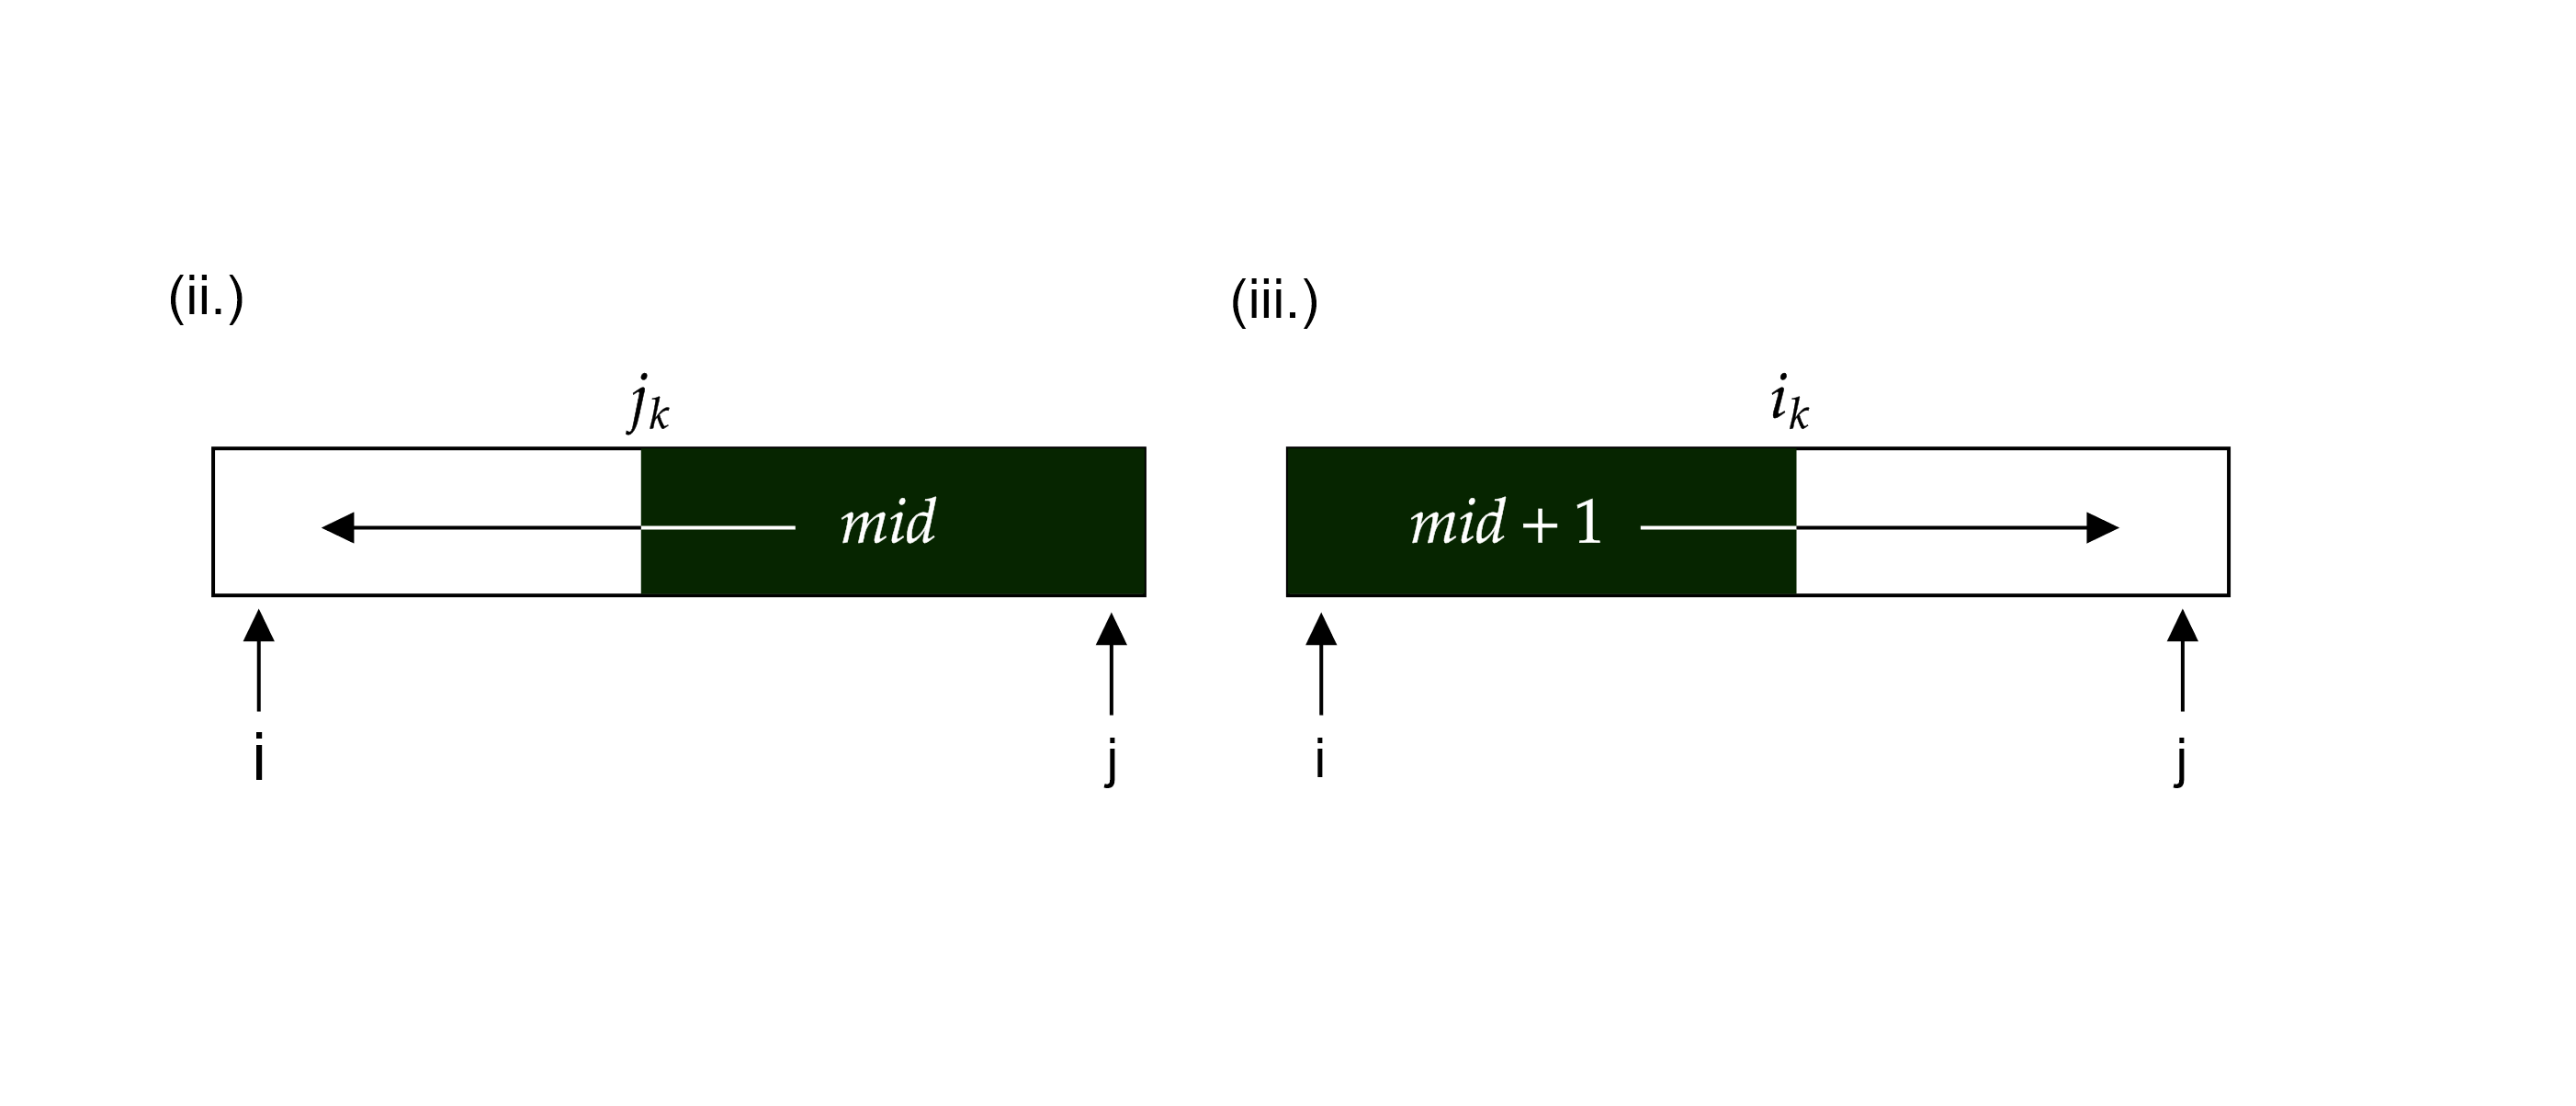
\includegraphics[width=1\textwidth]{sections/modules/recursive_evaluation/msort_proof.png}

    \vspace{-4em}
    \noindent
    Then in (ii.), the right bound $mid$ keeps decreasing, and in (iii.), the left bound $mid$ keeps increasing.
    This shirks both sub-arrays until both bounds meet. The merge function sorts after both calls, taking the next 
    biggest in the sub-arrays, placing it in the temporary array, and copying back to the original array. Hence, by induction, the function is correct.
\end{Proof}

\newpage

\begin{theo}[Iterative Substitution Method (plug-and-chug)]

    Given a function $T(n)$ which has a recurrence relation---meaning it calls 
    upon itself in its own definition---we may repeatedly substitute such self-references
    back into $T(n)$.

    Given that $T(n)$ properly subdivides to a base case $T(x)$, we may derive some
    pattern which illustrates the state of $T(n)$ at some depth $k$ within the recurrence.
    Doing so, we identify what makes our $k_{th}$ expression hit $T(x)$.
\end{theo}
\begin{Proof}[Iterative Substitution Method (plug-and-chug) - MergeSort]

    Merge sort has the recurrence relation $T(n) = 2T(n/2) + \Theta(n)$, for which the base case is $T(1)$.
    We substitute $T(n/2)$ into $T(n)$:
    \begin{align*}
        T(n) &= 2T(n/2) + \Theta(n);\quad \text{ and }\quad T(n/2) = 2T(n/2^2) + \Theta(n/2);\\
        T(n) &= 2\left[\hspace{3em} \right] + \Theta(n)\text{; Prepare to substitute the recurrence $T(n/2)$}\\
         &= 2\left[2T(n/2^2) + \Theta(n/2)\right] + \Theta(n);\text{ we evaluate $2\cdot\Theta\left(n/2\right)$ as $\Theta\left(2n/2\right)$}\\
         &= 2^2T(n/2^2) + \Theta(n) + \Theta(n)\text{; Simplified}\\
    \end{align*}

    \vspace{-1.5em}
\noindent
We won't fully simplify to observe how the recurrence builds. We continue, evaluating $T(n/2^2)$:
\begin{align*}
    T(n/2^2) &= 2T(n/2^3) + \Theta(n);\\
    T(n) &= 2^2\left[2T(n/2^3) + \Theta(n/2^2)\right] + \Theta(n)+\Theta(n);\text{substitute again}\\
    &= 2^3T(n/2^3) + \Theta(n)+\Theta(n)+\Theta(n)\text{; Simplified}\\
\end{align*}

\vspace{-1.5em}
\noindent
We identify the pattern for the $k_{th}$ substitution:
\begin{align*}
    T(n) &= 2^kT(n/2^k) + k\cdot\Theta(n)\text{; General form}\\
\end{align*}

\vspace{-1.5em}
\noindent
Now we identify what makes our recurrence $T(n/2^k) = T(1)$, i.e., where is $n/2^k = 1$, then $n=2^k$, and $\log_2 n = k$. We plug this back into our general form:
\begin{align*}
    T(n) &= 2^{\log_2 n}T(n/2^{\log_2 n}) + \log_2 n\cdot \Theta(n)\text{; Substituting $k$}\\
    &= n\Theta(1) + \log_2 n\cdot\Theta(n);\text{ Where $T(1)=\Theta(1)$}\\
    &= \Theta(n) + \Theta(n)\log_2 n;\\
    &= \Theta(n\log n);
\end{align*}
Hence, merge sort has a time complexity of $O(n\log n)$.

\end{Proof}

\begin{Tip}
    Live Demo: \url{https://youtu.be/Ob8SM0fz6p0?si=Z4PZQDWOXa7deEHA}
\end{Tip}
% \newpage
\section{Computers \& Number Base Systems}
 

\begin{Def}[Turing Machine]

    A \textbf{Turing Machine} is a theoretical computational model used to describe the capabilities of a general-purpose \textbf{computer}. It consists of an infinite tape (memory) and a read/write head processing symbols on the tape, one at a time, according to a set of predefined rules. The machine moves left or right, reading or writing symbols, and changing states based on what it reads. 
    
    The machine \textbf{halts} once it reaches a final state or continues indefinitely. Serving as a flexible, \textbf{higher-order function} (a function which receives functions).
\end{Def}

\begin{Def}[Von Neumann Architecture]

    Modern computers operate on a model known as the \textbf{Von Neumann architecture}, which consists of three primary components:
    \begin{enumerate}
        \item \textbf{Memory}: Stores data and instructions as sequences of bits.
        \item \textbf{Arithmetic and Logic Unit (ALU)}: Executes operations such as addition, subtraction, multiplication, and division on numbers stored in memory.
        \item \textbf{Control Unit}: Directs the execution of instructions and manages the flow of data between memory and the ALU.
    \end{enumerate}
    
    \noindent
    Where numbers are stored in memory cells, each cell holding an integer value represented in a fixed base, typically \(B = 2\), meaning \textbf{binary}. Where each digit is less than the base \(B\). We represent integers in memory as:
    
    \[
    a = \sum_{i=0}^{k-1} a_i B^i
    \]
    
    \noindent
    where \( a_i \) represents the individual digits, and \(B\) is the base. For large integers, computations may require manipulating several memory cells to store the full number.
\end{Def}

\noindent
\textbf{Example:} Consider the integer $a = 13$, and let us represent it in base $B = 2$ (binary). We can express this number as a sum of powers of $2$, corresponding to the binary representation of $13$:
    
\[
a = 1 \cdot 2^3 + 1 \cdot 2^2 + 0 \cdot 2^1 + 1 \cdot 2^0 = 8 + 4 + 0 + 1 = 13
\]

\noindent
In binary, this is represented as the sequence of digits: $a = (1101)_2$. Here, the coefficients $a_3 = 1$, $a_2 = 1$, $a_1 = 0$, and $a_0 = 1$ correspond to the binary digits of $13$.

\noindent
Similarly, if we want to represent $a = 45$ in base \textbf{$B = 10$ (decimal)}, we write:

\[
a = 4 \cdot 10^1 + 5 \cdot 10^0 = 40 + 5 = 45
\]

\noindent
In this case, the coefficients $a_1 = 4$ and $a_0 = 5$ correspond to the decimal digits of $45$.


\begin{Def}[Hexadecimal]
    
        \textbf{Hexadecimal} base $B=16$, using digits 0-9 and the letters A-F, where $A=10$, $B=11$, $C=12$, $D=13$, $E=14$, and $F=15$. Hexadecimal is commonly used in computing due to its compact representation of binary data. For example, a \textbf{byte} (8 bits) can be represented as two hexadecimal digits, simplifying the display of binary data.
\end{Def}


\begin{theo}[Base $2\leftrightarrow16$ Conversion]

    Let bases \( B:=2 \) (binary) and \( H:=16 \) (hexadecimal). At a high-level:

    \vspace{.5em}
    
    \noindent \textbf{Binary to Hexadecimal:}
    \begin{enumerate}
        \item Group $B$ digits in sets of 4, right to left. \textbf{Pad} leftmost group with 0's if necessary for a full group.
        \item Compute each group, replacing the result with their $H$ digit.
        \item Finally, combine each $H$ group.
    \end{enumerate}
    
    \noindent \textbf{Hexadecimal to Binary:}
    \begin{enumerate}
        \item Convert each $H$ digit into a 4 bit $B$ group.
        \item Finally, combine all $B$ groups.
    \end{enumerate}
    \noindent
    Additionally we may also trim any leading 0's.
\end{theo}

\noindent
\textbf{Example:}
    \begin{itemize}
        \item Binary to Hexadecimal:
        \[
        101101111010_2 \quad \Rightarrow \quad \text{Group as } ([1011] \ [0111] \ [1010]) \quad \Rightarrow \quad B7A_{16}
        \]
        \item Hexadecimal to Binary:
        \[
        3F5_{16} \quad \Rightarrow \quad [0011]\ [1111]\ [0101]_2 \Rightarrow \quad 1111110101_2
        \]
        \noindent
    \end{itemize}
    \noindent

\newpage 

\noindent
The following definition is for completeness: applications of such a base are currently uncommon.
\begin{Def}[Unary]
    
    \textbf{Unary}, base $B=1$. A system where each number is represented by a sequence of $B$ symbols. Where the number $n$ is represented by $n$ symbols. Often used in theoretical computer science to prove the existence of computable functions.
\end{Def}
\noindent
\textbf{Example:} The number $5$ in unary is represented by $5$ symbols: $5 = \texttt{IIIII}$ or $2= \texttt{II}$. There is no concept of 0, the absence of symbols represents 0.\\
\begin{Def}[Most \& Least Significant Bit]
    
    In a binary number, the \textbf{most significant bit (MSB)} is the leftmost bit. The \textbf{least significant bit (LSB)} is the rightmost bit.
\end{Def}
\textbf{Example:} Consider this byte (8 bits), $[1111 \ 1110]_2$, the MSB = 1 and the LSB = 0.  

\begin{theo}[Adding Binary]

    We may use the add and carry method alike decimal addition:
    \textbf{Binary Addition Rules:}
    \begin{itemize}
        \item $0 + 0 = 0$
        \item $0 + 1 = 1$
        \item $1 + 0 = 1$
        \item $1 + 1 = 0 \quad (\text{add 1 to the next digit (left)})$
    \end{itemize}
    \noindent
    We call the last step, \textbf{carry}, as we carry our overflow to the next digit.
\end{theo}

    \noindent
    \textbf{Example:} Adding $0010\ 0011\ 0100_2$ and $0100_2$:
    \begin{equation*}
        \begin{array}{B3}
             1       &                             1000 &  \carry 0\textcolor{red}{1}00 \\
              {} + 0 &                             0001 &  0\textcolor{red}{1}00 \\ \hline
                   1 &                             1001 &  1000 \\
        \end{array}
        \end{equation*}
\noindent
Where $[1\ 1000\ 0100]_2 + [0\ 0001\ 0100]_2 = [1\ 1001\ 1000]_2$.

\newpage

\begin{theo}[Signed Binary Numbers - Two's Complement]
    
    In a \textbf{two's complement system}, an $n$-bit signed (positive or negative) binary number can represent values in the range $[-2^{n-1}, 2^{n-1}-1]$. Then by most significant bit (MSB):
    \begin{itemize}
        \item If MSB is 0, the number is positive;
        \item If MSB is 1, the number is negative.
    \end{itemize}
    \noindent
    \textbf{Conversion to Two's Complement :}
    \begin{enumerate}
        \item Take an unsigned binary number and invert all bits, turning 0's to 1's and 1's to 0's.
        \item Finally add 1 to the least significant bit.
    \end{enumerate}
\end{theo}
\textbf{Example:} Converting $-5$ into a 4-bit two's complement:
    \begin{align*}
        5 \rightarrow 0101 \quad & \text{(binary for 5)} \\
         1010 \quad & \text{(inverted)} \\
         1011 \quad & \text{(add 1)}
    \end{align*}
    Thus, $-5$ is represented as $1011$ in 4-bits under two's complement.

    
% 

\section{Computing Large Numbers}
\noindent
In this section we discuss algorithms for computing large numbers, but first we define 
algorithmically, addition, subtraction, multiplication, division, and modula.

\begin{Def}[Wordsize]

    Our machine has a fixed \textbf{wordsize}, which is how much each memory cell can hold. Systems like 32-bit or 64-bit can hold $2^{32}$ $(\approx$ 4.3 billion) or $2^{64}$ $(\approx$ 18.4 quintillion) bits respectively.\\

    \noindent
    We say the ALU can performs arithmetic operations at $O(1)$ time, within wordsize. Operations beyond this size we deem \textbf{large numbers}.
\end{Def}
\noindent
The game we play in the following algorithms is to compute large integers without exceeding wordsize. Moving forward, we assume our machine is a typical 64-bit system.
\begin{Func}[Length of digits - $\|a\|$]

    We will use the notation $\|a\|$ to denote the number of digits in the integer $a$. For example, $\|123\| = 3$ and $\|0\| = 1$.
\end{Func}

\newpage
\begin{Def}[Computer Integer Division]

    Our ALU  \underline{only returns the quotient after division.} We denote the quotient as $\floor*{a/b}:a,b\in\Z$.
\end{Def}

\noindent
Our first hurdle is long division as , which will set up long addition and subtraction for success.

\noindent
\textbf{Scenario - Grade School Long Division:} Goes as follows, take $\frac{a}{b}$. Find how times $b$ fits into $a$ evenly, $q$ times. Then $a-bq$ is our remainder $r$.\\
\textbf{Examples:} let $a=\{12,5,17,40,89\}$, $b=\{4,2,3,9,10\}$ respectively, and base $B=10$,
\begin{center}
    (1.)\intlongdivision{12}{4} (2.)\intlongdivision{5}{2} (3.)\intlongdivision{17}{3} (4.)\intlongdivision{40}{9} (5.)\intlongdivision{89}{10} 
\end{center}
\noindent
Take (3.), $a=17$, $b=3$: 3 fits into 17 five times, which is 15. 17 take away 15 is 2, our remainder. We 
create an algorithm to compute this process.\\

\noindent
\textbf{Key Observation:} Consider the following powers of 2 of form $x=2^n+s$, where $x,n,s\in\Z$:
\begin{align*}
    3 = 2 + 1 &= 0000 \ 00\textcolor{red}{11}_2 \quad (1) \\
    6 = 4 + 2 &= 0000 \ 0\textcolor{red}{11}0_2 \quad (2) \\
    12 = 8 + 4 &= 0000 \ \textcolor{red}{11}00_2 \quad (3) \\
    24 = 16 + 8 &= 000\textcolor{red}{1} \ \textcolor{red}{1}000_2 \quad (4) \\
    48 = 32 + 16 &= 00\textcolor{red}{11} \ 0000_2 \quad (5) \\
    96 = 64 + 32 &= 0\textcolor{red}{11}0 \ 0000_2 \quad (6) \\
    192 = 128 + 64 &= \textcolor{red}{11}00 \ 0000_2 \quad (7)
\end{align*}

\noindent
Notice that as we increase the power of 2, the number of bits shift left towards a higher-order bit. Now, instead of calculating powers of 
2, we shift bits left or right, to yield instantaneous results.

\begin{theo}[Binary Bit Shifting (Powers of 2)]

    \label{theo:bit_shift}

    Let $x$ be a binary unsigned integer. Where ``$\ll$'' and ``$\gg$'' are left and right bit shifts:\\
    \noindent
    \textbf{Left Shift by $k$ bits:} $x \ll k:= x \cdot 2^k$\\
    \noindent
    \textbf{Right Shift by $k$ bits:} $x \gg k = \left\lfloor x/2^k \right\rfloor$\\
    \textbf{Remainder:} bits pushed out after right shift(s).
\end{theo}

\newpage
\noindent
\textbf{Example:} Observe, $16=10000$ (4 zeros), $8=1000$ (3 zeros), we shift by 4 and 3 respectively:
\begin{itemize}
    \item Instead of $3 \cdot 16$ in base 10, we can $3 \ll 4=48$, as $3 \cdot 2^4 = 48$.
    \item Conversely, Instead of $48/16$ in base 10, $48 \gg 4 = 3$, as $\floor*{48/2^4} = 3$.
    \item Catching the remainder: say we have $37/8$ base 10, then,
        \[ 37 = 100101_2 \quad \text{and} \quad 8 = 1000_2 \text{ then } 37 \gg 3 = 4 \text{ remainder } 5,\]

    \noindent    
    as  $[100101]$ $\gg$ 3 = [000100]101, where $101_2$ is our remainder $5_{10}$.
\end{itemize}

\begin{Func}[Division with Remainder in Binary (Outline) - \textit{QuoRem()}]

    \label{func:QuoRem}

    For binary integers, let dividend $a = (a_{k-1} \cdots a_0)_2$ and divisor $b = (b_{\ell-1} \cdots b_0)_2$ be unsigned, with $k \geq 1$,
    $\ell \geq 1$, ensuring $0 \leq b \leq a$, and $b_{\ell-1} \neq 0$, ensuring $b > 0$.\\ 
    
    \noindent
    We compute $q$ and $r$ such that, $a = bq + r$ and $0 \leq r < b$. 
    Assume $k \geq \ell$; otherwise, $a < b$. We set $q \gets 0$ and $r \gets a$. 
    Then quotient $q = (q_{m-1} \cdots q_0)_2$ where $m := k - \ell + 1$.\\

    \noindent
    \textbf{Input:} $a, b$ (binary integers)\\
    \noindent
    \textbf{Output:} $q, r$ (quotient and remainder in binary)\\
    \begin{algorithm}[H]
        \SetAlgoLined
        \SetKwProg{Fn}{Function}{:}{\KwRet{$(q, r)$;}}
        \Fn{\textit{QuoRem}($a, b$)}{
            $r \gets a$\;
            $q \gets \{0_{m-1} \cdots 0\}$\;
            \vspace{.5em}
            \For{$i \gets \|a\|-\|b\|-1$ $\textbf{\text{down to}}$ $0$}{
                $q_i \gets \left\lfloor \dfrac{r}{b \ll i} \right\rfloor$\; 
                $r \gets r - (q_i \cdot (b \ll i))$\;  
            }
          
        }
    \end{algorithm}
    \noindent\rule{\textwidth}{0.4pt}
    \noindent

    \noindent
    \textbf{Time Complexity}: $O(\|a\|(\|a\| - \|b\|))$. In short, line 5 we preform division on $\|a\|$ bits of decreasing size. 
    Though \textbf{not totally necessary}, For more
    detail visit \url{https://shoup.net/ntb/ntb-v2.pdf} on page 60. General $n$ cases can be found in Theorem (\ref{theo:basic-arithmetic}).
\end{Func}

\noindent
\textbf{Example} Let $a = 47_{10} = 101111_2$ and $b = 5_{10} = 101_2$, we run \textit{QuoRem($a,b$)}. We summarize the above example as, ``How many times does $101_2$ fit into $101111_2$?''
\begin{enumerate}
    \item  Does $5\ll 3$ fit into $101000_2$? It fits! $q=1000_2$, $r = 101111_2 - 101000_2$.
    \item  Does $5\ll 2$ fit into $0111_2$? no fits! $q=1000_2$, $r = 0111_2$.
    \item  Does $5\ll 1$ fit into $0111_2$? no fits! $q=1000_2$, $r = 0111_2$.
    \item  Does $5\ll 0$ fit into $0111_2$? It fits! $q=1001_2$, $r = 0111_2-0101$.
    \item  Return $q=1001_2=9_{10}$, $r = 0010 = 2_{10}$ 
\end{enumerate}

\newpage



\noindent
Long addition: We craft an algorithm for
grade school long addition, which goes as follows:
\begin{equation*}
    \begin{array}{@{}B2}
        \carry 2 5 & 3\carry 0  8 \\
                 {} + 39 &                  406 \\ \hline
                      64 &                  714 \\
    \end{array}
    \end{equation*}
\noindent
Where adding, $25,308 + 39,406 = 64,714$. We create an algorithm to compute this in the following function.\\

\noindent
Here the function $QuoRem$ (\ref{func:QuoRem}) to return (quotient, remainder) preforms in $O(1)$ as bits are small enough for word size.
\begin{Func}[Addition of Binary Integers - \textit{Add()}]
    Let $a = (a_{k-1} \cdots a_0)_2$ and $b = (b_{\ell-1} \cdots b_0)_2$ be unsigned binary integers, where $k \geq \ell \geq 1$. We compute $c := a + b$ where the result $c = (c_{k}c_{k-1} \cdots c_0)_2$ is of length $k+1$, assuming $k \geq \ell$. If $k < \ell$, swap $a$ and $b$. This algorithm computes the binary representation of $a + b$.

    \vspace{.5em}
    \noindent
    \textbf{Input:} $a, b$ (binary integers)\\
    \textbf{Output:} $c = (c_k \cdots c_0)_2$ (sum of $a + b$)\\

    \begin{algorithm}[H]
        \SetAlgoLined
        \SetKwProg{Fn}{Function}{:}{\KwRet{}}
        \Fn{\textit{Add}($a, b$)}{
            $carry \gets 0$\;
            \For{$i \gets 0$ \textbf{to} $\ell - 1$}{
                $tmp \gets a_i + b_i + carry$\;
                $(carry, c_i) \gets \texttt{QuoRem}(tmp, 2)$\;
            }
            \For{$i \gets \ell$ \textbf{to} $k - 1$}{
                $tmp \gets a_i + carry$\;
                $(carry, c_i) \gets \texttt{QuoRem}(tmp, 2)$\;
            }
            $c_k \gets carry$\;
            \KwRet{$c = (c_k \cdots c_0)_2$}\;
        }
    \end{algorithm}
    \noindent\rule{\textwidth}{0.4pt}

    \noindent
    \textbf{Note:} $0 \leq \textit{carry} \leq 1$ and $0 \leq \textit{tmp} \leq 3$.\\
    \textbf{Time Complexity:} $O(\max(\|a\|,\|b\|))$, as we iterate at most the length of the largest input.\\
    \textbf{Space Complexity:} $O(\|a\|+\|b\|)$, though $c = k+1$, constants are negligible as $k, \ell \to \infty$.
\end{Func}

\newpage

\noindent
For subtracting, $5,308 - 3,406 = 1,904$, where we borrow 10 from the 5 to make 13:
\begin{equation*}
    \begin{array}{@{}B2}
         \not{\carry[4]5} & \carry[10] 3 0  8 \\
                 {} - 3 &                  406 \\ \hline
                      1 &                  904 \\
    \end{array}
\end{equation*}

\vspace{-1em}
\begin{Func}[Subtraction of Binary Integers - \textit{Subtract()}]
    Let \( a = (a_{k-1} \cdots a_0)_2 \) and \( b = (b_{\ell-1} \cdots b_0)_2 \) be unsigned binary integers, where \( k \geq \ell \geq 1 \) and \( a \geq b \). We compute \( c := a - b \) where the result \( c = (c_{k-1} \cdots c_0)_2 \) is of length \( k \), assuming \( a \geq b \). If \( a < b \), swap \( a \) and \( b \) and set a negative flag to indicate the result is negative. This algorithm computes the binary representation of \( a - b \).
    
    \vspace{.5em}
    \noindent
    \textbf{Input:} \( a, b \) (binary integers)\\
    \textbf{Output:} \( c = (c_{k-1} \cdots c_0)_2 \) (difference of \( a - b \))
    
    \begin{algorithm}[H]
        \SetAlgoLined
        \SetKwProg{Fn}{Function}{:}{\KwRet{}}
        \Fn{\textit{Subtract}($a, b$)}{
            $borrow \gets 0$\;
            \For{$i \gets 0$ \textbf{to} $\ell - 1$}{
                $tmp \gets a_i - b_i - borrow$\;
                \eIf{$tmp < 0$}{
                    $borrow \gets 1$\;
                    $c_i \gets tmp + 2$\;
                }{
                    $borrow \gets 0$\;
                    $c_i \gets tmp$\;
                }
            }
            \For{$i \gets \ell$ \textbf{to} $k - 1$}{
                $tmp \gets a_i - borrow$\;
                \eIf{$tmp < 0$}{
                    $borrow \gets 1$\;
                    $c_i \gets tmp + 2$\;
                }{
                    $borrow \gets 0$\;
                    $c_i \gets tmp$\;
                }
            }
            \KwRet{$c = (c_{k-1} \cdots c_0)_2$}\;
        }
    \end{algorithm}
\noindent\rule{\textwidth}{0.4pt}

\noindent
\textbf{Note:} $0\leq borrow\leq 1$. Subtraction may produce a borrow when $a_i < b_i$.\\
\textbf{Time Complexity:} \( O(\max(\|a\|, \|b\|)) \), iterating at most the length of the largest input.\\
\textbf{Space Complexity:} \( O(\|a\| + \|b\|) \), as the length of \( c \) is at most \( k \), with constants negligible as \( k, \ell \to \infty \).
\end{Func}
    


\newpage

\noindent
For multiplication, $24\cdot 16= 384$:
\begin{equation*}
    \begin{array}{@{}B2}
                                            &  \carry[2]24 \\
                 {} \times  &                  16 \\ \hline
                 {}   &                  144 \\ 
                 {} +  &                  240 \\ \hline
                       &                  384 \\
    \end{array}
\end{equation*}
\noindent
Where $6\cdot 4 = 24$, we write the 4 and carry the 2. Then $6\cdot 2 = 12$ plus the carried 2 is 14. Then we multiply the next digit, 1, we add a 0 below our 144, and repeat the process. Every new 10s place we add a 0. Then we add our two products to get 384.\\

\noindent
We create an algorithm to compute this process in the following function:
\begin{Func}[Multiplication of Base-$B$ Integers - \textit{Mul()}]
    \label{func:mul}
    Let $a = (a_{k-1} \cdots a_0)_B$ and $b = (b_{\ell-1} \cdots b_0)_B$ be unsigned integers, where $k \geq 1$ and $\ell \geq 1$. The product $c := a \cdot b$ is of the form $(c_{k+\ell-1} \cdots c_0)_B$, and may be computed in time $O(k\ell)$ as follows:

    \vspace{.5em}
    \noindent
    \textbf{Input:} $a, b$ (base-$B$ integers)\\
    \textbf{Output:} $c = (c_{k+\ell-1} \cdots c_0)_B$ (product of $a \cdot b$)\\

    \begin{algorithm}[H]
        \SetAlgoLined
        \SetKwProg{Fn}{Function}{:}{\KwRet{}}
        \Fn{\textit{Mul}($a, b$)}{
            \For{$i \gets 0$ \textbf{to} $k + \ell - 1$}{
                $c_i \gets 0$\;
            }
            \For{$i \gets 0$ \textbf{to} $k - 1$}{
                $carry \gets 0$\;
                \For{$j \gets 0$ \textbf{to} $\ell - 1$}{
                    $tmp \gets a_i \cdot b_j + c_{i+j} + carry$\;
                    $(carry, c_{i+j}) \gets \texttt{QuoRem}(tmp, B)$\;
                }
                $c_{i+\ell} \gets carry$\;
            }
            \KwRet{$c = (c_{k+\ell-1} \cdots c_0)_B$}\;
        }
    \end{algorithm}

    \noindent\rule{\textwidth}{0.4pt}
    
    \noindent
    \textbf{Note:} At every step, the value of \textit{carry} lies between $0$ and $B-1$, and the value of \textit{tmp} lies between $0$ and $B^2 - 1$.\\
    \textbf{Time Complexity:} $O(\|a\|\cdot\|b\|)$, since the algorithm involves $k \cdot \ell$ multiplications.\\
    \textbf{Space Complexity:} $O(\|a\| + \|b\|)$, since we store the digits of $a$, $b$, and $c$.
\end{Func}



\newpage
\begin{Func}[Decimal to Binary Conversion - \textit{DecToBin()}]
    This function converts a decimal number $n$ into its binary equivalent by repeatedly dividing the decimal number by 2 and recording the remainders.

    \vspace{.5em}
    \noindent
    \textbf{Input:} $n$ (a decimal number)\\
    \textbf{Output:} $b$ (binary representation of $n$)\\

    \begin{algorithm}[H]
        \SetAlgoLined
        \SetKwProg{Fn}{Function}{:}{\KwRet{}}
        \Fn{\textit{DecToBin}($n$)}{
            $b \gets \text{empty string}$\;
            \While{$n > 0$}{
                $r \gets n \bmod 2$\;
                $n \gets \left\lfloor \frac{n}{2} \right\rfloor$\;
                $b \gets r \ + \ b$\; % Prepend the remainder to the binary string
            }
            \KwRet{$b$}\;
        }
    \end{algorithm}
    \noindent\rule{\textwidth}{0.4pt}
    
    \noindent
    \textbf{Time Complexity:} $O(\log n)$, as the number of iterations is proportional to the number of bits in $n$.\\
    \textbf{Space Complexity:} $O(n)$, storing our input $n$.
\end{Func}

\noindent
\textbf{Example:} Converting 89 to binary given the above function:
\begin{align*}
    89_{10} &\div 2 = 44 \quad \text{rem} \ 1, \longleftarrow \textbf{ LSB}&   \\
    44_{10} &\div 2 = 22 \quad \text{rem} \ 0,& \\
    22_{10} &\div 2 = 11 \quad \text{rem} \ 0,& \\
    11_{10} &\div 2 = 5 \quad \ \text{rem} \ 1,& \\
    5_{10} &\div 2 = 2 \quad \ \text{rem} \ 1,& \\
    2_{10} &\div 2 = 1 \quad \ \text{rem} \ 0,& \\
    1_{10} &\div 2 = 0 \quad \ \text{rem} \ 1.  \longleftarrow \textbf{ MSB} &  
\end{align*}
Thus, $89_{10} = 1011001_2$.

\begin{theo}[Time Complexity of Basic Arithmetic Operations]
    
    \label{theo:basic-arithmetic}

    We generalize the time complexity to $a$ and $b$ as $n$-bit integers. 
    \begin{enumerate}
        \item [(i)] \textbf{Addition \& Subtraction:} $a \pm b$ in time $O(n)$.
        \item [(ii)]\textbf{Multiplication:} $a \cdot b$ in time $O(n^2)$.
        \item [(iii)]\textbf{Quotient Remainder} quotient $q := \left\lfloor \frac{a}{b} \right\rfloor: b \neq 0, a>b;$ and remainder $r := a \mod b$ has time $O(n^2)$.
    \end{enumerate}
\end{theo}
% \section{Computational Efficiency}

\begin{theo}[Binary Length of a Number - $\|a\|$]
    
    The binary length of an integer $a_{10}$ in binary representation, is given by:
    
    \[
    \|a\| := 
    \begin{cases} 
    \lfloor \log_2 |a| \rfloor + 1 & \text{if } a \neq 0, \\
    1 & \text{if } a = 0,
    \end{cases}
    \]
    
    \noindent
    as $\lfloor \log_2 |a| \rfloor + 1$ correlates to the highest power of 2 required to represent $a$.
\end{theo}

\noindent
\textbf{Example:} Think about base 10 first. Let there be a 9 digit number $d=684,301,739$.
To reach 9 digits takes $10^8$; The exponent plus 1 yields $\|d\|$. Hence, $\lfloor \log_{10} d\rfloor+1$ is $\|d\|$.\\

\noindent
Now, let there be a 7 digit binary number $b=1001000$, which expanded is:
$$ (1\cdot 2^6) + (0\cdot 2^5) + (0\cdot 2^4) + (1\cdot 2^3) + (0\cdot 2^2) + (0\cdot 2^1) + (0\cdot 2^0) = 72,$$
\noindent
Taking $6$ powers of 2 to reach $72$, we add 1 to get $\|b\| = 7$. Hence, $\|b\| = \lfloor \log_2 b \rfloor + 1$.

\noindent
Additionally, if $a=0_2$ then $\|a\|=1$. as $a^0=1$.\\

\noindent

\begin{theo}[Splitting Higher and Lower Bits]

    Let $a$ be a binary number with $n$ bits. We can split $a$ into two numbers $A_1$ and $A_0$ with $n/2$ bits each,
    representing the first and second halves respectively. Where:
    
        $$A_1:=\frac{a}{2^{\ceil{n/2}}} \quad \text{ and } \quad A_0:=a \text{ mod } 2^{\ceil{n/2}}$$

\end{theo}

\noindent
\textbf{Example:} Let's start with base 10. To achieve $A_1=7455$ and $A_0=62,010$, for $a=745,562,010$.
we take the length $\|a\|:=\floor{\log_{10}(745,562,010)}+1=9$, as $10^8\leq 745,562,010<10^9$. Then:
\[ A_1=\frac{745,562,010}{10^{\ceil{9/2}}}=7455, \quad \text{ and } \quad A_0=745,562,010 \text{ mod } 10^{\ceil{9/2}}=62,010 \]
\noindent
as $10^5\leq 62,010<10^6$. Likewise to finding the remainder in base 2, we can use the same bit shifting technique for base 10 (\ref{theo:bit_shift}).
We see,
$$[745,562,010]_{10} \text{ right shift by 5, } [000,007,455]_{10}\ 62,010.$$ 

\noindent
Hence, $62,010$ is pushed out, and our remainder. Then, we can apply the same technique to base 2.
Let $a=1111\ 1111\ 1001\ 1001_2$. We have $\|a\|:=16$, then:
\[ A_1=\frac{1111\ 1111\ 1001\ 1001_2}{2^{\ceil{16/2}}}=1111\ 1111_2 \text{, and } A_0=1111\ 1111\ 1001\ 1001_2 \text{ mod } 2^{\ceil{16/2}}=1001\ 1001_2 \]

\newpage
\noindent
\textbf{Scenario - \textit{Divide and Conquer Multiplication}:} We are to compute, 
\[A_1 2^{\ceil{n/2}}+A_0=:a \quad \times \quad b:= B_1 2^{\ceil{n/2}}+B_0.\]
\noindent
Then we have,
\begin{align*}
    a\cdot b &=(A_1 2^{\ceil{n/2}}+A_0)(B_1 2^{\ceil{n/2}}+B_0)\\
    &=(A_1 2^{\ceil{n/2}})(B_1 2^{\ceil{n/2}})+(A_1 2^{\ceil{n/2}})B_0+(B_1 2^{\ceil{n/2}})A_0+A_0B_0\\
    &=(A_1B_1)2^{n}+(A_1B_0+B_1A_0)2^{\ceil{n/2}}+A_0B_0.
\end{align*}
\noindent
We need to compute 4 products, $(A_1B_1)$, $(A_1B_0), (B_1A_0)$, and $(A_0B_0)$. We now attempt to solve them independently:

\begin{Func}[Multiplication of $n$-bit Integers - \textit{Multiply()}]
    Let $a$ and $b$ be $n$-bit integers of base 2. This algorithm recursively computes the product of $a$ and $b$ using a straightforward divide-and-conquer approach, without using Karatsuba's optimization.

    \vspace{.5em}
    \noindent
    \textbf{Input:} $n, a, b$ (where $a$ and $b$ are $n$-bit integers)\\
    \textbf{Output:} The product $a \times b$\\

    \begin{algorithm}[H]
        \SetAlgoLined
        \SetKwProg{Fn}{Function}{:}{\KwRet{}}
        \Fn{\textit{Multiply}($n, a, b$)}{
            \If{$n < 2$}{
                \textbf{return} the result of grade-school multiplication for $a \times b$\;
            }
            \Else{
                $A_1 \gets a \div 2^{n/2};\ A_0 \gets a \bmod 2^{n/2}$\;
                $B_1 \gets b \div 2^{n/2};\ B_0 \gets b \bmod 2^{n/2}$\;

                \vspace{.5em}
                $p_1 \gets \textit{Multiply}(n/2, A_1, B_1)$\;
                $p_2 \gets \textit{Multiply}(n/2, A_1, B_0)$\;
                $p_3 \gets \textit{Multiply}(n/2, A_0, B_1)$\;
                $p_4 \gets \textit{Multiply}(n/2, A_0, B_0)$\;

                \textbf{return} $p_1 \cdot 2^n + (p_2 + p_3) \cdot 2^{n/2} + p_4$\;
            }
        }
    \end{algorithm}
    \noindent\rule{\textwidth}{0.4pt}

    \noindent
    \textbf{Time Complexity:} $O(n^2)$, as in our master method $T(n)=4T(n/2)+O(n)$, Theorem (\ref{theo:master}).\\
    \textbf{Space Complexity:} $O(n)$, storing $n+n$ bits for $a$ and $b$, while we track $O(\log_2 n)$ depth in the recursion stack.
\end{Func}
\noindent
We appear to make no improvement, however there's a small trick to reduce the number of multiplications. We continue on the next page.

\newpage

\noindent
Observe our full term, $c:=(\textcolor{red}{A_1B_1})2^{n}+(\textcolor{blue}{A_1B_0+B_1A_0})2^{\ceil{n/2}}+\textcolor{red}{A_0B_0}.$ Say we computed another term,
\[z:=(A_1+A_0)(B_1+B_0)=(\textcolor{red}{A_1B_1})+\textcolor{blue}{(A_1B_0)+(B_1A_0)}+(\textcolor{red}{A_0B_0}).\]
\noindent
Notice how $z$ also contains $(A_1B_1)$ and $(A_0B_0)$, which are also in $c$. Say
$m=(A_1B_0)+(B_1A_0)$. Let $x:=(A_1B_1)$ and $y:=(A_0B_0)$ then $z-x-y=m$. This reduces the number of multiplications to 3, as we only compute
 $(A_1B_1)$, $(A_0B_0)$ once, and then $z$.\\

\noindent
We employ the above strategy, which is \textbf{Karatsuba's multiplication algorithm}:

\begin{Func}[Karatsuba's Multiplication Algorithm - \textit{KMul()}]
    Let $a$ and $b$ be $n$-bit integers of base 2. This algorithm recursively computes the product of $a$ and $b$ using a divide-and-conquer approach.

    \vspace{.5em}
    \noindent
    \textbf{Input:} $n, a, b$ (where $a$ and $b$ are $n$-bit integers)\\
    \textbf{Output:} The product $a \times b$\\

    \begin{algorithm}[H]
        \SetAlgoLined
        \SetKwProg{Fn}{Function}{:}{\KwRet{}}
        \Fn{\textit{Multiply}($n, a, b$)}{
            \If{$n < 2$}{
                \textbf{return} the result of grade-school multiplication for $a \times b$\;
            }
            \Else{
                $A_1 \gets a \div 2^{n/2};\ A_0 \gets a \bmod 2^{n/2}$\;
                $B_1 \gets b \div 2^{n/2};\ B_0 \gets b \bmod 2^{n/2}$\;

                \vspace{.5em}
                $x \gets \textit{Multiply}(n/2, A_1, B_1)$\;
                $y \gets \textit{Multiply}(n/2, A_0, B_0)$\;
                $z \gets \textit{Multiply}(n/2, A_1 + A_0, B_1 + B_0)$\;

                \textbf{return} $x \cdot 2^n + (z - x - y) \cdot 2^{n/2} + y$\;
            }
        }
    \end{algorithm}
    \noindent\rule{\textwidth}{0.4pt}

    \noindent
    \textbf{Time Complexity:} $O(n^{\log_2 3}) \approx O(n^{1.585})$, as in our master method $T(n)=3T(n/2)+O(n)$, Theorem (\ref{theo:master}).\\
    \textbf{Space Complexity:} $O(n)$.
\end{Func}


% \chapter{Networking Fundamentals}
% \vspace{-1em}
\section{The Internet}

\noindent
Terminology and concepts of the internet, which will be used throughout this text.

\begin{Def}[Protocol]

    A \textbf{protocol} is a set of rules which govern the exchange of data between devices. 
    Protocols define the format, timing, sequencing, and error control of data transmission \cite{rfc791}.
\end{Def}

\begin{Def}[Internet]

    The \textbf{Internet} is a global network of distributed system communicating over an \textbf{Internet Protocol} (IP) \cite{cloudflare_internet_protocol}.
    Documents served over the internet are referred to as \textbf{webpages} or \textbf{websites}.
\end{Def}
\begin{Def}[HTTP \& HTML]

    \textbf{HTTP} (HyperText Transfer Protocol), the protocol which transfer data over the internet, 
    distributing \textbf{HTML} (HyperText Markup Language) documents. Such 
    documents include \textbf{hyperlinks} to other websites, images, and other media \cite{rfc9110}.
\end{Def}
\begin{Def}[RFC (Request for Comments)]

    \textbf{RFC} (Request for Comments) is a publication from the \textbf{Internet Engineering Task Force} (IETF) 
    and the \textbf{Internet Society} (ISOC). This body governs the specifications for the internet and its protocols \cite{rfc}.
\end{Def}

\begin{Def}[DNS and IP Addresses]

    An \textbf{Internet Protocol address} (IP address) is a unique identifier for a device on a network. 
    The \textbf{Domain Name System} (DNS) maps domain names to IP addresses \cite{rfc760}.
\end{Def}

\newpage

\begin{Def}[Web Browser]

    A \textbf{web browser} is a software application for accessing the \textbf{World Wide Web} (WWW) \cite{ou_internet_history}.
\end{Def}

\begin{Def}[URL (Uniform Resource Locator)]

    A \textbf{URL} (Uniform Resource Locator) references each webpage, specifying protocol, domain, and path \cite{w3c_html_href_draft}.
    E.g., \texttt{http://www.example.com/path/to/resource}.
    \begin{itemize}
        \item \textbf{Protocol}: \texttt{http}
        \item \textbf{Domain}: \texttt{www.example.com}
        \item \textbf{Path}: \texttt{/path/to/resource}
    \end{itemize}
\end{Def}
\begin{Def}[Client-Server Model]

    Most of the internet operates on a \textbf{client-server model}, where an agent device\textendash the \textbf{client}\textendash requests data from another agent\textendash the \textbf{server}\textendash 
    which serves an appropriate response. Clients are not servers and vice versa, as they receive and interpret data differently \cite{cloudflare_client_server}.
\end{Def}

\begin{Def}[HTTP Methods]
    
        When a client makes a request to a server, they must specify their intent, categorized by \textbf{HTTP methods} \cite{rfc2616}:
        \begin{itemize}
            \item \textbf{GET}: Retrieve data from the server.
            \item \textbf{POST}: Send data to the server.
            \item \textbf{PUT}: Update data on the server.
            \item \textbf{DELETE}: Remove data from the server.
        \end{itemize}
\end{Def}
\begin{Def}[HTTP Headers]

    \textbf{HTTP headers} are key-value pairs sent between the client and server to provide \textbf{metadata} about the request or response.
    \textbf{Metadata} is data about the transmitted data, telling the receiver how the incoming data should be interpreted \cite{rfc2616}.
\end{Def}


\newpage
\noindent
Tim Berners-Lee and his team at CERN developed the first web server and browser in 1989 \cite{w3c_http_history}.

\begin{table}[h!]
    \centering
    \begin{tabular}{@{}p{3cm}p{10cm}@{}}
    \toprule
    \textbf{HTTP Version} & \textbf{Description} \\ \midrule
    HTTP/0.9 (1991)       & Only supports GET method (retrieving HTML alone). \\
    HTTP/1.0 (1996)       & RFC\#1945, adding support for metadata in HTTP headers, status codes, and POST and HEAD methods \cite{rfc1945}. \\
    HTTP/1.1 (1997)       & Defined in RFC\#2068 and later updated by RFC\#2616, introduced persistent connections, chunked transfer encoding, and additional cache control mechanisms \cite{rfc2068}\cite{rfc2616}. \\
    HTTP/2 (2015)         & RFC\#7540, improving performance by enabling request and response multiplexing, header compression, and prioritization \cite{rfc7540}. \\
    HTTP/3 (2022)         & Builds upon HTTP/2's features and uses the QUIC transport protocol to reduce latency and improve security. \cite{rfc9114} \\ \bottomrule
    \end{tabular}
    \caption{Evolution of HTTP Versions}    
    \label{tab:http_versions}
\end{table}

\begin{Note}
    \textbf{Note:} In short, \textbf{Persistent Connections} allow multiple requests and responses to be sent over a single connection, reducing latency and improving performance \cite{rfc2616}.
    \textbf{Chunked Transfer Encoding} allows the server to send data in chunks, enabling the client to start processing data before the entire response is received \cite{rfc2616}.
    \textbf{Multiplexing}, is the ability to send multiple requests and responses over a single connection, reducing latency and improving performance \cite{multiplexing_networkencyclopedia}. 
     \textbf{QUIC} will be discussed alter on with other transfer protocols in a later section.

\end{Note}

\section{Data Transmission}
This section details how internet traffic is transmitted between devices.
\begin{Def}[ISO Model]

    The \textbf{ISO model} (International Organization for Standardization) is a conceptual framework for transmitted data between devices. 
    It is divided into seven layers of function\cite{ibm_osi_model}. Published in 1984 by the International Organization for Standardization (ISO) \cite{kanade_osi_model}.

\end{Def}
\begin{Def}[TCP/IP Model]

    The \textbf{TCP/IP model} (Transmission Control Protocol/Internet Protocol)
    is a concise representation of the ISO model used in practical settings \cite{yasar_tcpip}.
\end{Def}

\newpage


\begin{Def}[ISO Layers]

    \begin{enumerate}
        \item \textbf{Physical}: Converts data into physical signals (e.g., electrical, optical, or radio waves) for transmission across the network medium (e.g., cables, fiber optics, or wireless channels).
        \item \textbf{Data Link}: local delivery of directly connected devices within \textbf{Local Area Networks} (LAN) using \textbf{Media Access Control} (MAC) addresses for 
        addressing.
        \item \textbf{Network}: Handles addressing, routing, in external networks from source to destination.
        \item \textbf{Transport}: Ensures end-to-end delivery, via a message delivery protocol.
        \item \textbf{Session}: Initiates and terminates network connections, ensuring efficient resource usage.
        \item \textbf{Presentation}: To translate, compress, and encrypt data  (e.g., Operating Systems).
        \item \textbf{Application}: User facing services such as, HTTP , FTP, DNS, SMTP, etc.
    \end{enumerate}
    \hfill \cite{leonard_osi_model}\cite{Rayes2022}
\end{Def}

\begin{Note}
    \textbf{Note:} Many of the above layers are closely related, if not identical. 
    In practice, layers 5-6 are integrated into layer 7, and 
    layers 1-2 are often combined into a single layer in the TCP/IP model.
    
\end{Note}


\begin{Def}[TCP/IP Layers]

    \begin{enumerate}
        \item \textbf{Network Interface}: Physical and data link layers from ISO. 
        \item \textbf{Internet}: Attaches IP addresses to data packets for routing across the internet.
        \item \textbf{Transport}: Defines the delivery protocol, segmenting data into packets.
        \item \textbf{Application}: The Session, Presentation, and Application layers from ISO.
    \end{enumerate}
    \hfill \cite{Rayes2022}
\end{Def}

Despite the numbering of the layers, the user interacts with the application layer, which communicates down the chain
of layers to the physical layer, where the data is transmitted over the network medium. The receiving device then 
interprets the data, moving back up the chain to the application layer.

\newpage 

\noindent
To illustrate the contrast between the ISO and TCP/IP models, consider the diagram:
\begin{figure}[h!]
    \centering
    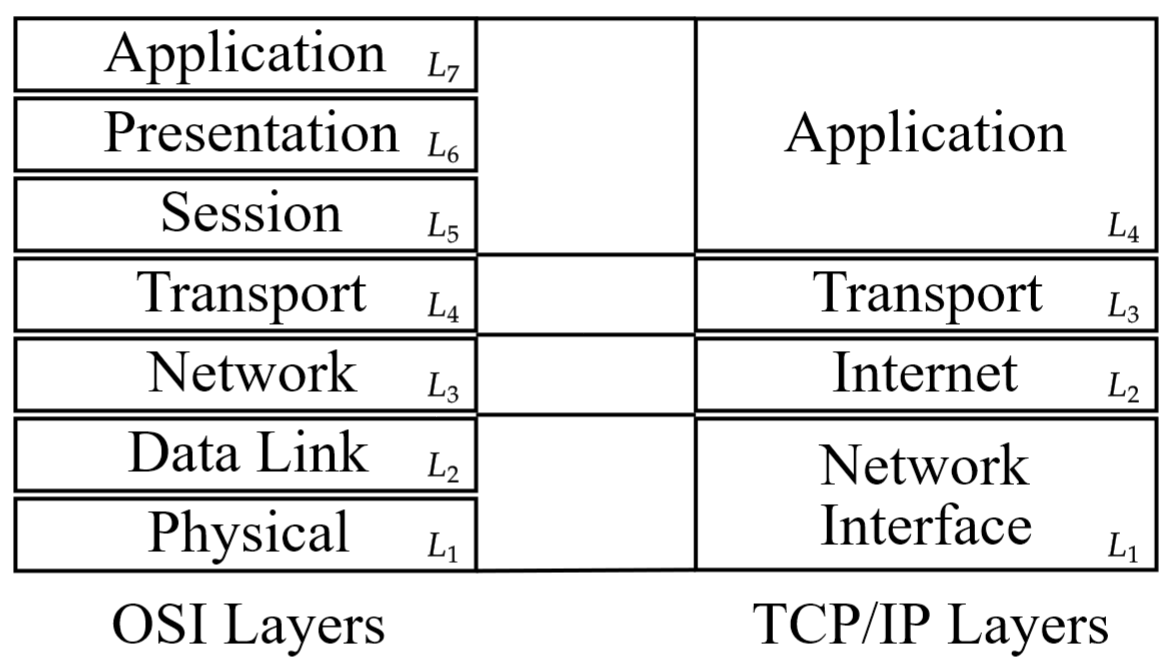
\includegraphics[width=0.7\textwidth]{Sections/network/osi_tcp.png}
    \caption{ISO vs TCP/IP Model}
    \label{fig:osi_tcpip}
\end{figure}

To illustrate two devices communicating over the internet, consider the diagram:

\section{Routing Networks}

\noindent
When IP addresses began


\begin{Def}[Routing]

    \textbf{Routing} is the process of selecting the best path across networks. 
    Data is segmented into packets, each with a destination address. 
    \textbf{Routers} are devices which forward this data through the network.

    Routers have a \textbf{routing table} which maps to other reachable networks. 
    When a packet arrives, the router checks against its routing table to find the best path.
    \hfill \cite{cloudflare_routing}
\end{Def}

\begin{Def}[Hop-by-Hop \& End-to-End Routing]

    \begin{itemize}
        \item  \textbf{Hop-by-Hop Routing}: When a packet of data is forwarded from one router to the next, a forward decision is called a \textbf{hop}.
        \item \textbf{End-to-End Routing}: The process of sending data from source to destination without intermediate hops.
    \end{itemize}
    \noindent
    It is often rare to see end-to-end routing in modern networks, as data is often forwarded through multiple routers. A target 
    destination may be unreachable from a given router.
    \hfill \cite{heimlicher_e2e_hbh}
\end{Def}

\newpage

\begin{Def}[Router Advertising]

    When routers inform each other of their existence and the networks they can reach \cite{narten_rfc4861}.
\end{Def}
\begin{Def}[Routing Protocols]
    
    \begin{itemize}
        \item \textbf{IP} (Internet Protocol): The primary protocol for routing data across the internet.
        \item \textbf{BGP} (Border Gateway Protocol): The protocol for routing data between \textbf{Autonomous Systems} (AS). 
        an AS is a collection of IP networks and routers under the control of a single entity (e.g., an \textbf{ISP} (Internet Service Provider)).
        These may only connect with each other if they have a mutual agreement. ASes identify themselves to 
        external networks using a unique \textbf{Autonomous System Number} (ASN).
        These are unique 16 bit numbers between 1-65534 or 32 bit numbers between 131072-4294967294 (e.g., \texttt{AS12345}) \cite{cloudflare_autonomous_system}.
        \item \textbf{OSPF} (Open Shortest Path First): A link-state routing protocol used within an AS. Link-state protocols are a set 
        of algorithms which determine the best path, based on the topology of a network graph \cite{kurose_link_state_routing}.
        It is also an \textbf{IGP} (Interior Gateway Protocol), meaning it operates within a single AS. It does so by sending out \textbf{LSAs} (Link State Advertisements) to other routers in the AS.
        Then routers in the system build a \textbf{LSADB} (Link State Advertisement Database) of the network topology. Then a shortest path algorithm is run to determine the best path to each network \cite{certbros_ospf_explained}.
        \item \textbf{RIP} (Routing Information Protocol): RIP employs hop count as a routing metric, with a maximum allowable hop count of 15 (network size limitation).
        It operates as an \textbf{IGP} within a single AS, periodically broadcasting the entire routing table to neighboring routers every 30 seconds,
        which can lead to slower convergence and higher bandwidth usage compared to other protocols. RIP is largely deprecated \cite{javatpoint_rip_protocol}.
    \end{itemize}
\end{Def}

\begin{Def}[IP Addressing]

    \textbf{IP addresses} are unique identifiers for devices on a network. 
    There are two versions of IP addresses, \textbf{IPv4} and \textbf{IPv6}.
    IPv4 A 32-bit address ($2^{32}$ addresses), employed since 1983, quickly exhausted all available addresses by the 2010s \cite{info12060246}.
    IPv6 is a 128-bit address ($2^{128}$ addresses), introduced in 1998 , in an attempt to address this shortage \cite{deering_ipv6_specification}\cite{ibm_ipv4_ipv6_formats}.
    For example,
    \begin{itemize}
        \item \textbf{IPv4}: a decimal octet ``$x.x.x.x$'': $x \in [0, 255]$ (e.g., \texttt{192.168.1.1}).
        \item \textbf{IPv6}: a hexadecimal segment ``$y:y:y:y:y:y:y:y$'': $y\in [0, FFFF]$ \\
         (e.g., \texttt{2001:0db8:85a3:0000:0000:8a2e:0370:7334}).
    \end{itemize}
\end{Def}

\newpage

\begin{Def}[Subnetting]

    Instead of a large monolith network of routers, networks can be divided into 
    smaller networks called \textbf{subnets}. I.e., Instead of passing data to every device on a network, routers forward data to a representative device on each subnet.
    \hfill \cite{cloudflare_subnet}
\end{Def}
\begin{Def}[Subnet Masking]

    A \textbf{subnet mask} defines which part of an IP address identifies the \textbf{network} and which part identifies the \textbf{host}.
\end{Def}
\begin{Def}[Classful Network]

    In the beginning, the first octet of an IPv4 address determined the network class---only allowing for 256 networks.
    The RFC\#791 published in 1981 introduced \textbf{Classful Networks} \cite{postel_internet_protocol}. 
    It uses the first three bits of the first octet's binary representation as a subnet mask to determine a class ranging from A-E---D and E were rarely if ever used.
\end{Def}

\begin{table}[h!]
    \centering
    \begin{tabular}{@{}p{.1cm}p{1.1cm}p{2cm}p{3cm}p{4cm}@{}}
    \toprule
    \textbf{Class} & \textbf{Binary Prefix} & \textbf{Range (Decimal)} & \textbf{Purpose} & \textbf{Details} \\ \midrule
    A              & \texttt{0xx}           & 1.0.0.0 to 126.0.0.0     & Unicast (large networks) & For large organizations; 8 bits for the network, 24 for hosts. \\
    B              & \texttt{10x}           & 128.0.0.0 to 191.255.0.0 & Unicast (medium networks) & For medium-sized networks; 16 bits for the network, 16 for hosts. \\
    C              & \texttt{110}           & 192.0.0.0 to 223.255.255.0 & Unicast (small networks) & For small networks; 24 bits for the network, 8 for hosts. \\
    D              & \texttt{1110}          & 224.0.0.0 to 239.255.255.255 & Multicast & Reserved for multicast addressing; not for general use. \\
    E              & \texttt{1111}          & 240.0.0.0 to 255.255.255.255 & Experimental and future use & Reserved for research and development; not assigned for standard use. \\ \bottomrule
    \end{tabular}
    \caption{Overview of IPv4 Address Classes}
    \label{tab:ipv4_classes}
\end{table}






\newpage 

\noindent 

\begin{Def}[Fixed Length Subnet Masking (FLSM)]

    \textbf{Fixed Length Subnet Masking} (FLSM) is a technique which divides a network into equal-sized subnets. This
    may lead to inefficient use of IP addresses.
    \hfill \cite{awati_vlsm}
\end{Def}
\begin{Def}[Variable Length Subnet Masking (VLSM)]

    \textbf{Variable Length Subnet Masking} (VLSM) is a technique which allows for the creation of subnets with different sizes. 
    As some ASes may require more IP addresses than others, VLSM allows for more efficient use of IP addresses.
    \hfill \cite{awati_vlsm}
\end{Def}
\noindent

\begin{Def}[Classless Inter-Domain Routing (CIDR)]

    \textbf{Classless Inter-Domain Routing} (CIDR), introduced in 1993 through RFC\#1518 and RFC\#1519 to address IPv4 exhaustion.
    \textbf{CIDR replaced classful subnetting} with VLSM.

    \noindent
    CIDR notation is written as \underline{\texttt{IP Address/Prefix Length} (e.g., \texttt{192.168.1.0/24})}, where:
    \begin{itemize}
        \item \texttt{IP Address}: Represents the starting address of the network.
        \item \texttt{Prefix Length}: The number of bits used for the \textbf{network portion} of the address.\\
    \end{itemize}

    \vspace{-1em}
    \noindent
    For example:\\

        \vspace{-1em}
        \begin{center}
            \large
            \texttt{255.0.0.0\textbf{/8}}; \hspace{.2em} \texttt{255.255.0.0\textbf{/16}}; \hspace{.2em} \texttt{255.255.255.0\textbf{/24}}; \hspace{.2em} \texttt{255.255.255.192\textbf{/26}};
            \normalsize
        \end{center}
    \hfill \cite{fuller_cidr_rfc1519}
\end{Def}

\begin{Def}[Route Aggregation]

    CIDR introduced \textbf{Route Aggregation} also known as \textbf{Supernetting}, or \textbf{Route Summarization}, is the process of combining multiple routes into a single route advertisement.
    \textbf{Example}:
    Consider an organization assigned the following contiguous IP address blocks:
    \begin{center}
        \texttt{192.168.\textbf{1}.0/24}; \quad \texttt{192.168.\textbf{2}.0/24}; \quad \texttt{192.168.\textbf{3}.0/24}; \quad \texttt{192.168.\textbf{4}.0/24};
    \end{center}
    Each block holding 256 IP addresses with a subnet mask of 255.255.255.0, requiring four routing table entries. 
    However, these networks share a common prefix: the first 22 bits (\texttt{192.168.0.0/22}), which aggregates to: \texttt{\textbf{192.168.0.0/22}} \cite{fuller_cidr_rfc1519}.

\end{Def}
\newpage
\begin{Def}[IP Address Components]
    
        \item \textbf{Network Address}:
        \begin{itemize}
            \item Identifies the specific network segment to which a device is connected.
            \item Determined by setting all bits in the host portion to 0.
            \item Example: For the IP address \texttt{192.168.1.10} with a subnet mask of \texttt{255.255.255.0} (/24), the network address is \texttt{192.168.1.0}.
        \end{itemize}

        \item \textbf{Host Address}:
        \begin{itemize}
            \item Uniquely identifies a device within a network segment.
            \item The bits in the IP address designated for hosts, specified by the subnet mask.
            \item Example: In the IP address \texttt{192.168.1.10} with a /24 subnet mask, the host portion is the last octet (10).
        \end{itemize}

        \item \textbf{Broadcast Address}:
        \begin{itemize}
            \item Used to communicate with all devices on a specific network segment simultaneously.
            \item Determined by setting all bits in the host portion to 1.
            \item Example: For the network \texttt{192.168.1.0/24}, the broadcast address is \texttt{192.168.1.255}.
        \end{itemize}
      

    \hfill \cite{sunshine_rfc919} \cite{postel_rfc922} \cite{manning_rfc1878}

\end{Def}
\noindent
Consider the IP address \texttt{192.168.2.12/26} and its binary \texttt{11000000.10101000.00000010.00001100}:

\vspace{-1em}
\begin{figure}[h!]
    \hspace{2em}
    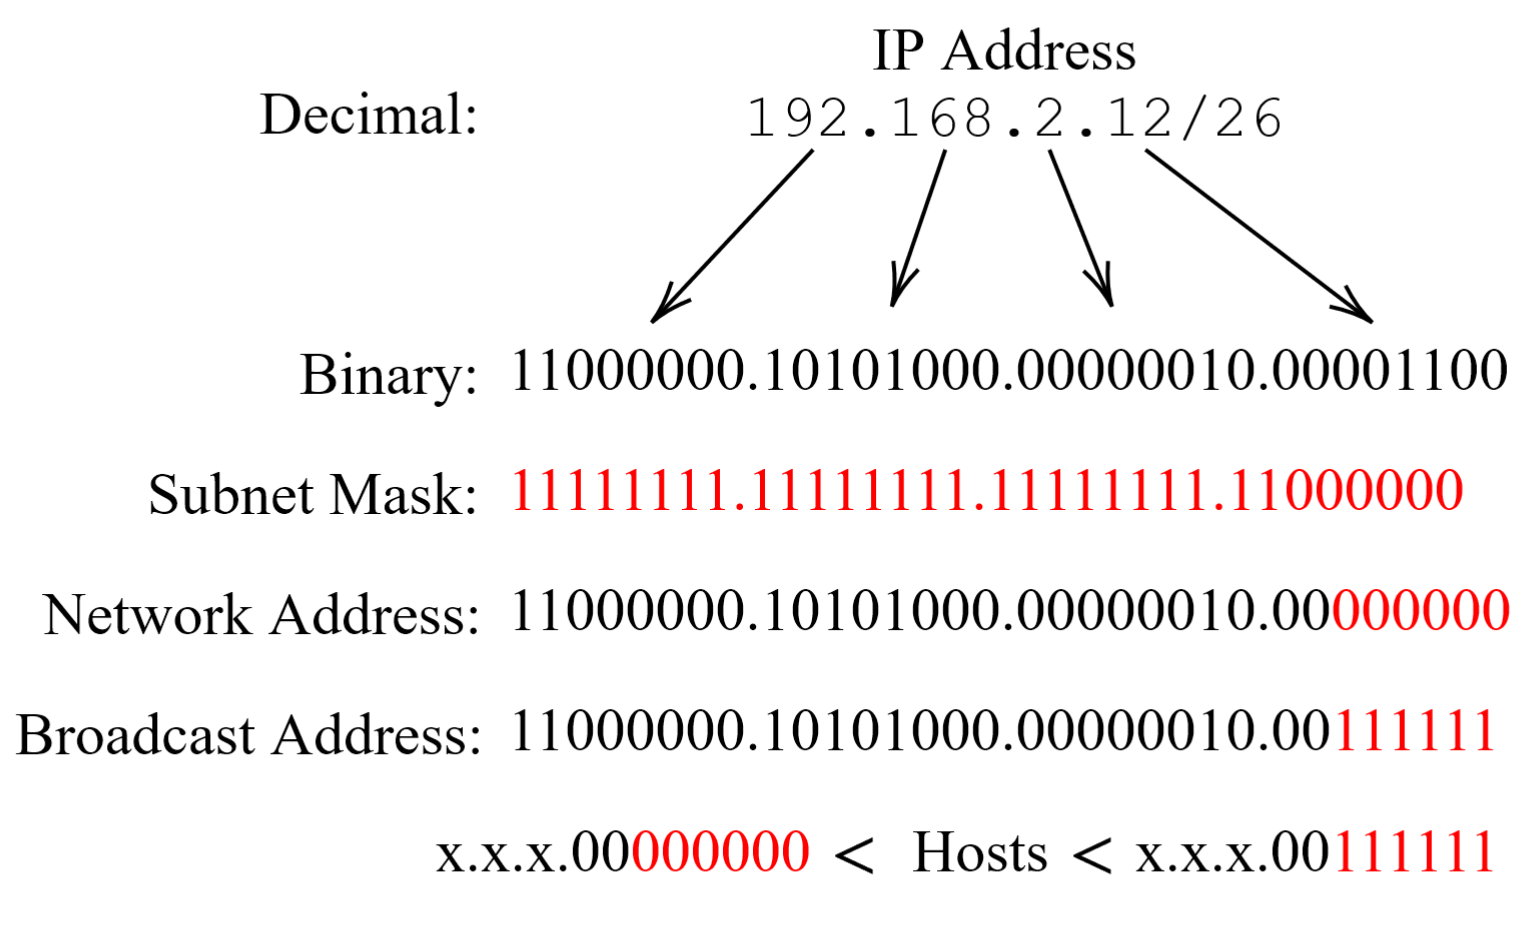
\includegraphics[width=0.7\textwidth]{Sections/network/ip_address.png}
    \caption{Binary Subnetting: Red indicating parts of the IP address identified for each component.}
    \label{fig:subnetting}
\end{figure}
\noindent
\begin{Def}[Common Types of Area Networks (ANs)]

    \textbf{PAN (Personal Area Network)}: A network for personal devices, such as smartphones, smartwatches, or earbuds, with a short range (typically a few meters) using technologies like Bluetooth or infrared.\\

    \noindent
    \textbf{LAN (Local Area Network)}: Connects devices within a small area, such as a home, office, or school, enabling high-speed communication and resource sharing.\\

    \noindent
    \textbf{WLAN (Wireless Local Area Network)}: A wireless version of LAN that uses Wi-Fi to connect devices within a localized area like a home or office.\\

    \noindent
    \textbf{CAN (Campus Area Network)}: A network that connects multiple LANs across a limited geographical area, such as a university campus or corporate facility, for resource sharing and communication.\\

    \noindent
    \textbf{MAN (Metropolitan Area Network)}: Covers a larger area than a LAN, typically a city or metropolitan region, connecting multiple LANs or CANs via high-speed infrastructure like fiber optics.\\

    \noindent
    \textbf{WAN (Wide Area Network)}: Connects LANs, MANs, or other networks over large geographical areas, such as countries or continents. The internet is the largest WAN example.\\

    \noindent
    \textbf{SAN (Storage Area Network)}: A high-speed network that provides access to storage devices for data centers, ensuring fast and reliable storage management.\\

    \noindent
    \textbf{EPN (Enterprise Private Network)}: A private network created by organizations to connect their various locations securely, often including VPNs for remote access.\\

    \noindent
    \textbf{VPN (Virtual Private Network)}: Creates a secure, encrypted connection over public networks, like the internet, to allow users to access private networks remotely.\\

    \noindent
    \textbf{HAN (Home Area Network)}: A network within a home environment, connecting personal devices like computers, printers, and smart home gadgets.\\

    \noindent
    \textbf{GAN (Global Area Network)}: A large-scale network that connects multiple WANs and supports worldwide communication, with the internet as its most prominent example.

    \hfill \cite{petryschuk_types_of_networks}
\end{Def}

\newpage 

\begin{Example}[Subnetting a Network via VLSM]


Consider the FLSM below, which all have 62 hosts per network:
\[
\begin{array}{|c|c|c|}
\hline
\textbf{Network Address} & \textbf{Hosts} & \textbf{Broadcast Address} \\ \hline
192.168.100.0 & .1 - .62 & .63 \\ \hline
192.168.100.64 & .65 - .126 & .127 \\ \hline
192.168.100.128 & .129 - .190 & .191 \\ \hline
192.168.100.192 & .193 - .254 & .255 \\ \hline
\end{array}
\]
\noindent
Below illustrates this network, where a router of base address \texttt{192.168.1.0/24},
connects four LANs:\\

\hspace{4em}
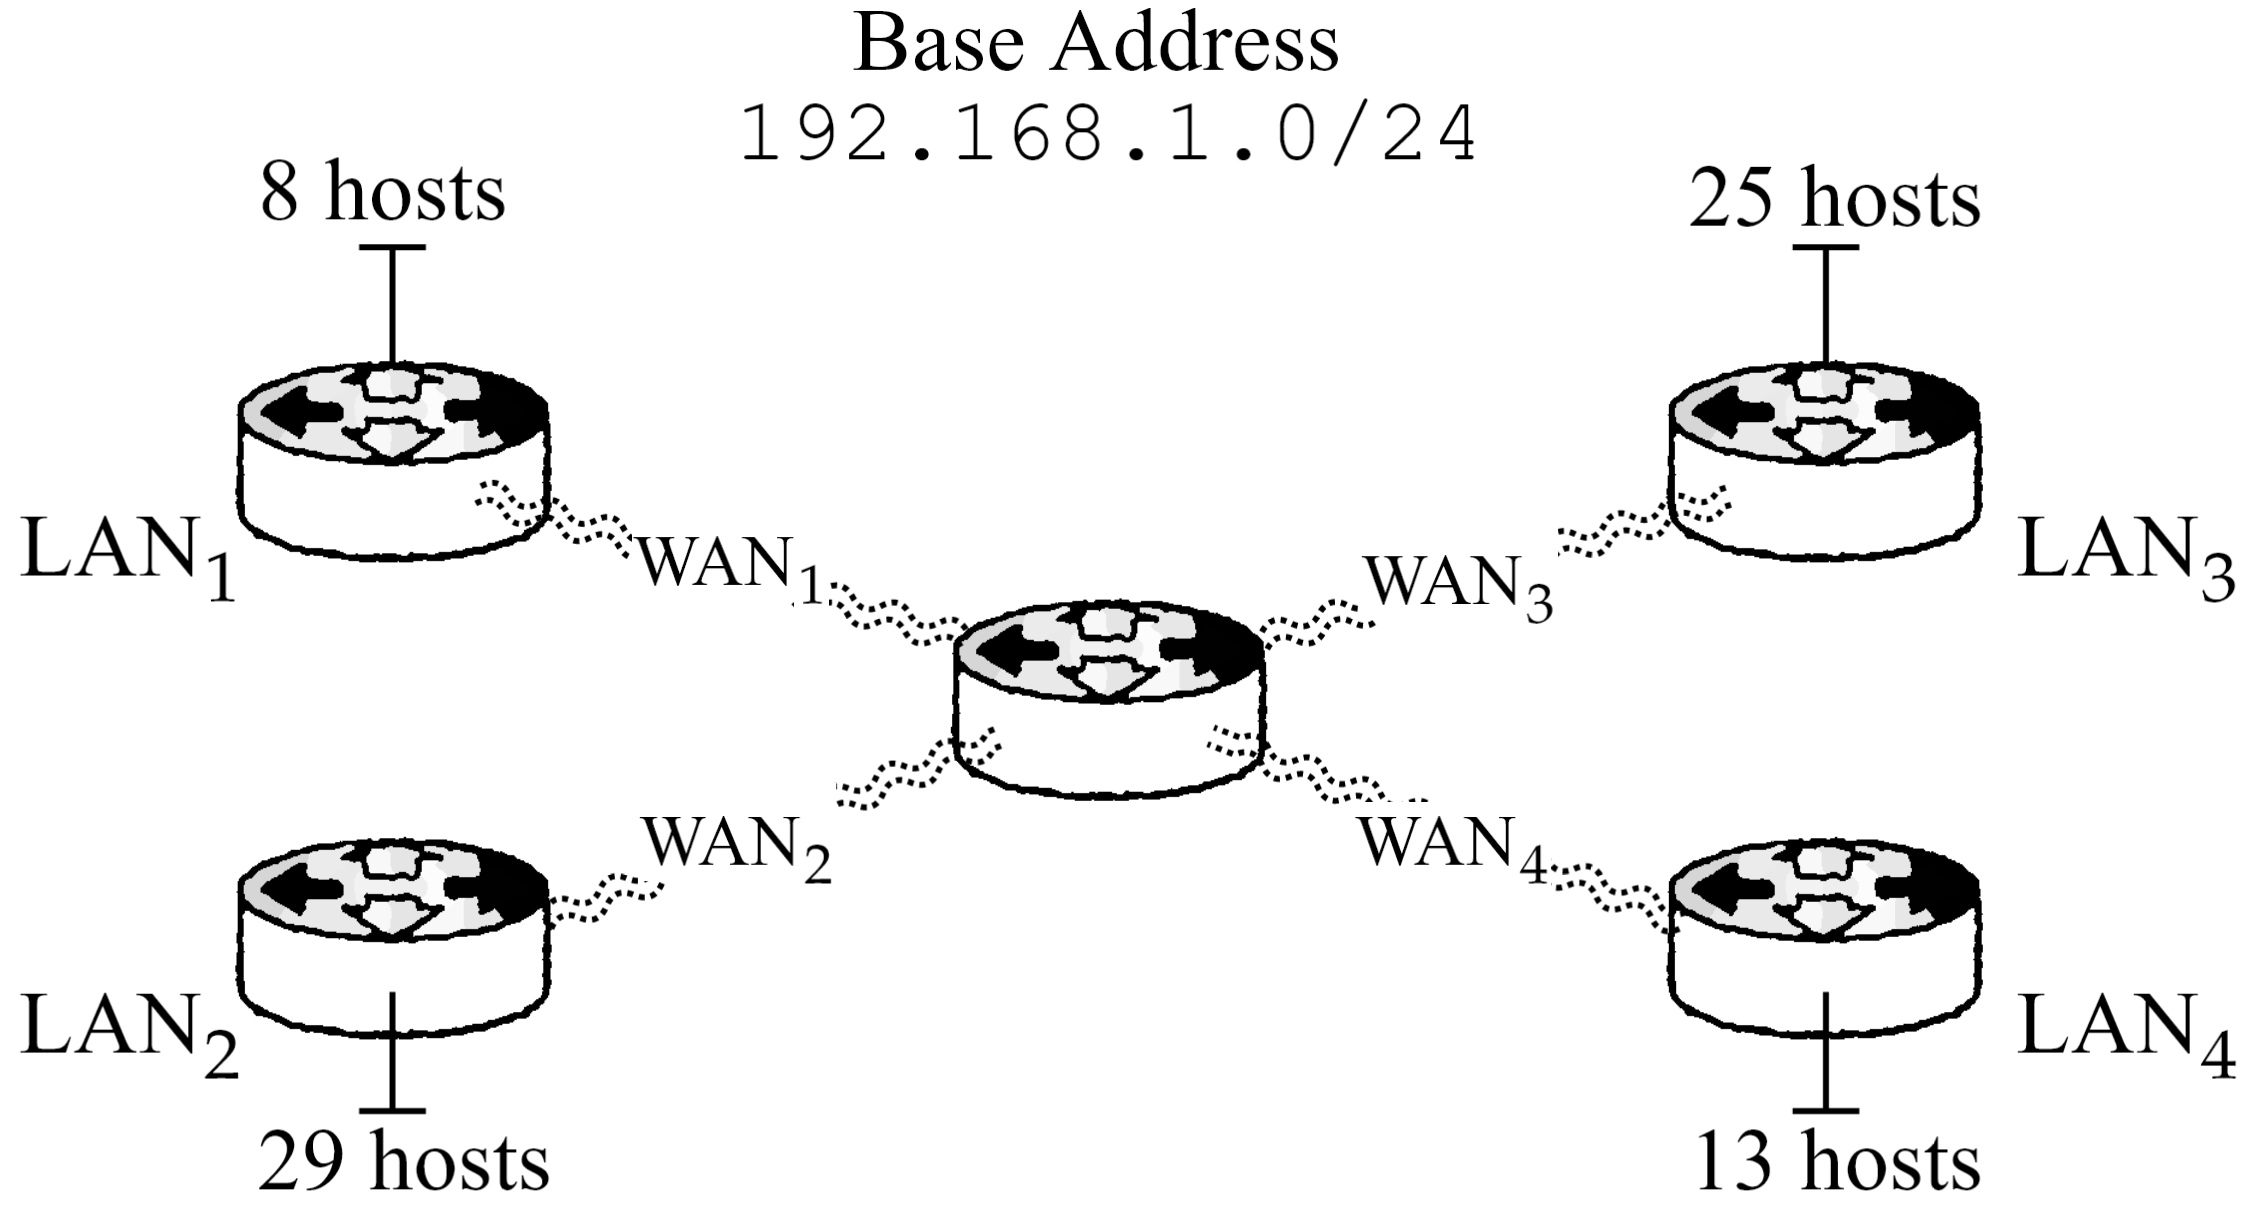
\includegraphics[width=0.7\textwidth]{Sections/network/subnetting.png}\\

\noindent
\textbf{Subnetting:} Process each LAN from largest to smallest, Select the nearest block size, identify the network, host, and broadcast addresses.
Since there is a subnet mask of /24, blocks $[128, 64, 32, 16, 8, 4, 2, 1]$ are available. This is the case as 
$2^8 = 256$. If a LAN has 129 hosts, that LAN will occupy all 256 addresses.\\
\begin{enumerate}
    \item \textbf{LAN$_2$}: 29 hosts $\Rightarrow$ Block size 32. Network: \texttt{x.0}, Broadcast: \texttt{x.31}, Hosts: \texttt{x.1-x.30}.
    \item \textbf{LAN$_3$}: 25 hosts $\Rightarrow$ Block size 32. Network: \texttt{x.32}, Broadcast: \texttt{x.63}, Hosts: \texttt{x.33-x.62}.
    \item \textbf{LAN$_4$}: 13 hosts $\Rightarrow$ Block size 16. Network: \texttt{x.64}, Broadcast: \texttt{x.79}, Hosts: \texttt{x.65-x.78}.
    \item \textbf{LAN$_1$}: 8 hosts $\Rightarrow$ Block size 16. Network: \texttt{x.80}, Broadcast: \texttt{x.95}, Hosts: \texttt{x.81-x.94}.
\end{enumerate}

\noindent
8 hosts need occupy 16, as a block size of 8 only has 6 usable addresses. The computed subnet now only occupies addresses 
\texttt{x.0-x.95}, leaving room for additional LANs \cite{eastcharmer_vlsm_subnetting}. 

\end{Example}
    





\chapter{Software Security \& Defenses}
\section{Document Certificates \& Binding Encryptions}
Before, all communication sent ``\textbf{over the wire}'' (from device to device),
was sent ``\textbf{in the clear}'' (unencrypted). This means that anyone could 
view data sent between devices in plain text. This is a problem when setting up 
infrastructure such as banking, e-commerce, or any other service that requires
sensitive information to be sent over the internet.

\label{sec:tls}
\begin{Def}[Integrity \& Authenticity]

    \textbf{Integrity} is the assurance that data has not been altered in transit.\\
    \textbf{Authenticity} is the assurance that the data is coming from the correct source.
\end{Def}
\begin{Def}[Transport Layer Security (TLS)]

    TLS is a protocol providing end-to-end encryption of data. It authenticates
    the server via \textbf{TLS certificates} to ensure the client is connecting to 
    the correct host. It also ensures integrity of the data.

    The Engineering Task Force (IETF) published the first version of TLS in 1999. As of 
    today the most recent version is TLS 1.3. (2018).
    \hfill \cite{cloudflare_tls}
\end{Def}

\begin{Def}[Secure Sockets Layer (SSL) [Deprecated]]

    SSL is the predecessor to TLS. It was developed by Netscape in the 1990s. 
    SSL 3.0 was released in 1996. SSL 3.0 was found to be insecure and was replaced
    by TLS 1.0 in 1999.
    \hfill \cite{cloudflare_tls}
\end{Def}

\begin{Def}[Certificate Authority (CA)]

    A CA is a third-party entity that issues digital certificates. Often called \textbf{SSL certificates} or TLS certificates.
    The protocol supports both SSL and TLS. Despite SSL's deprecation the name stuck due branding issues.
    Browsers and Operating systems have a list of trusted CAs called the \textbf{root store}.
    A full list of Microsoft's trusted CAs can be found here:\\ \href{https://ccadb.my.salesforce-sites.com/microsoft/IncludedCACertificateReportForMSFT}{https://ccadb.my.salesforce-sites.com/microsoft/...}
    \hfill \cite{kinsta_tls_ssl}
\end{Def}

\newpage 

\begin{Def}[Encryption]

    \textbf{Encryption} is the process of converting plaintext into ciphertext (indiscernible text).\\
    \textbf{Decryption} is the process of converting ciphertext back into plaintext.

\end{Def}
\begin{Def}[Symmetric \& Asymmetric Encryption]
    
    \textbf{Key}: is a seed/piece of information used to encrypt or decrypt data.\\
    \textbf{Symmetric Encryption}: uses the same key for both encryption and decryption.\\
    \textbf{Asymmetric Encryption}: uses a public key for encryption and a private key for decryption.\\
    ${}$ \hfill \cite{adetunji_symmetric_asymmetric_encryption}
\end{Def}

\vspace{-1em}
\begin{figure}[h!]
    \centering
    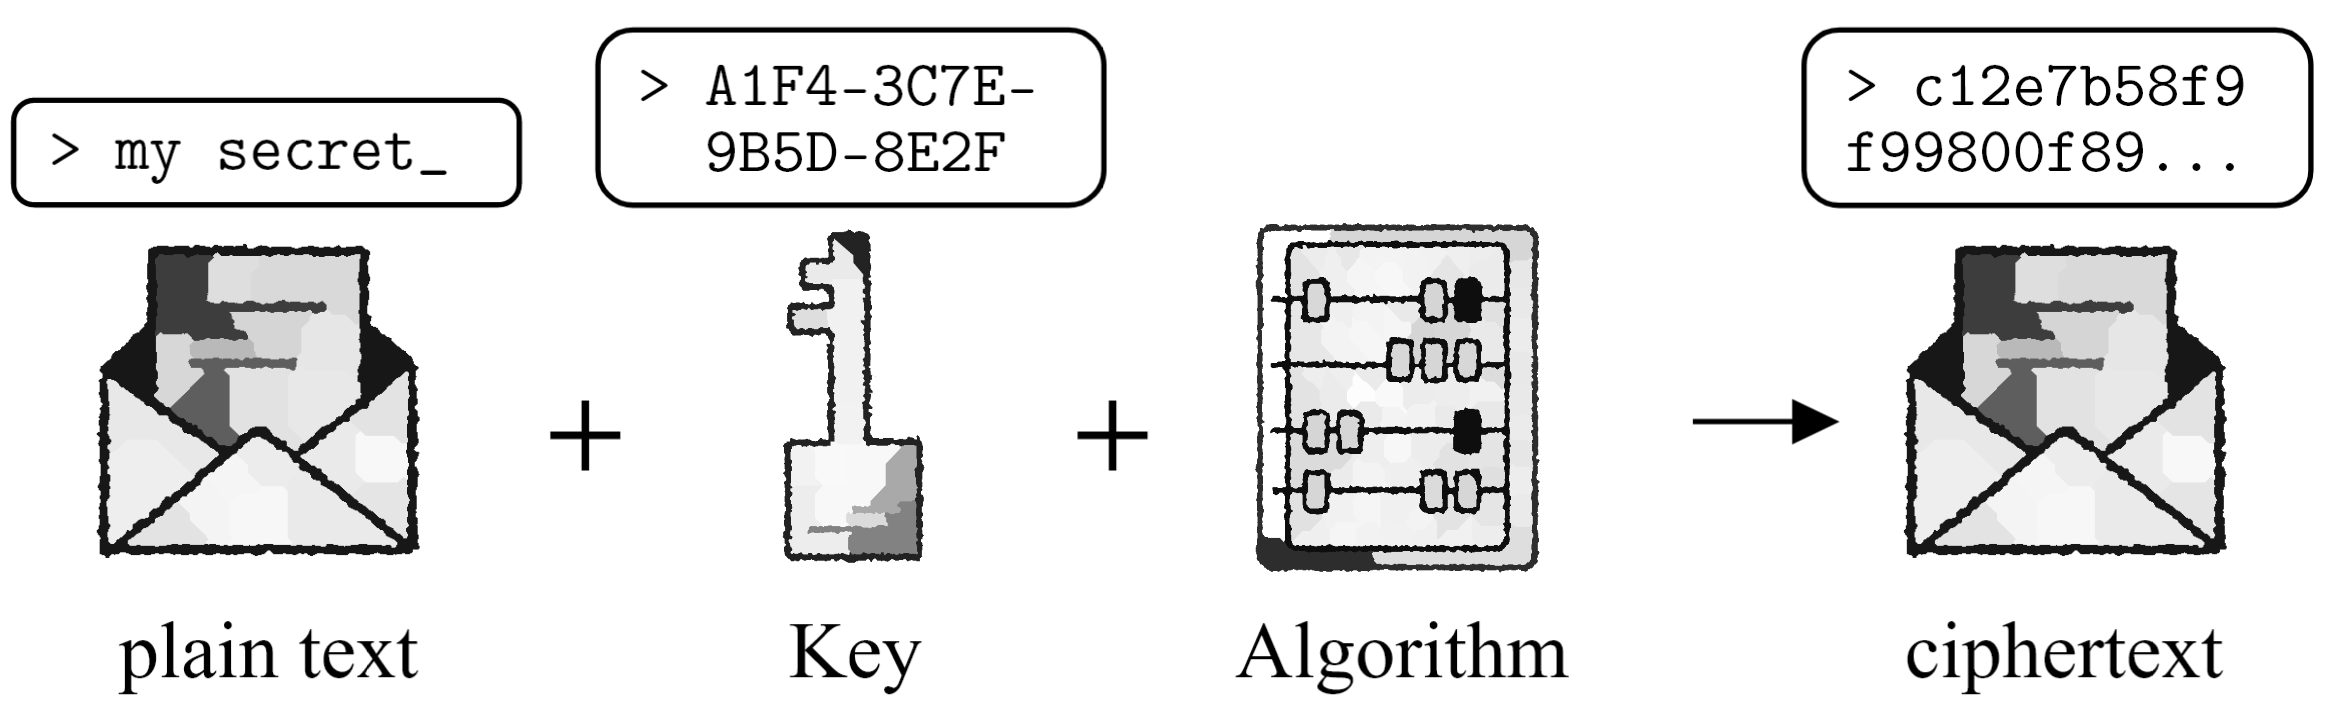
\includegraphics[width=1\textwidth]{Sections/sec/encrypt.png}
    \caption{High-level depiction of encryption.}
    \label{fig:encryption}
\end{figure}

\noindent
Encryption takes a key, data, and an algorithm to produce ciphertext.
Decryption takes the same key, ciphertext, and algorithm to produce the original data.

\vspace{1em}
\begin{Def}[Hashing]
    \textbf{Hashing} is the process of converting data into a fixed-length string of characters.
    Hashing is a one-way function, meaning it cannot be reversed (theoretically). In practice, 
    it is computationally infeasible to reverse a hash without brute force (trying all possible inputs) 
    or exploiting weaknesses in the hashing algorithm. The results of a hashing algorithm 
    is often called the \textbf{digest}. \hfill \cite{codecademy_hashing}
\end{Def}

\begin{Def}[Hypertext Transfer Protocol Secure (HTTPS)]

    A version of HTTP that uses TLS to encrypt data. \hfill \cite{cloudflare_http_not_secure}
\end{Def}


\newpage 
\begin{Def}[SSL/TLS Certificate Specifications]

    \begin{itemize}
        \item \textbf{Common Name (CN)}: The domain name the certificate is issued for.
        \item \textbf{Subject Alternative Name (SAN)}: Additional domain names or subdomains covered by the certificate.
        \item \textbf{Key Length}: A minimum of 2048 bits, ensuring strong encryption.
        \item \textbf{Hashing Algorithm}: Typically SHA-256 for secure data integrity.
        \item \textbf{Valid From/To}: The validity period, usually up to 397 days.
        \item \textbf{Issuer}: The trusted Certificate Authority (CA) that issued the certificate.
        \item \textbf{Extended Key Usage}: Specifies purposes like server authentication or client authentication.
    \end{itemize}
    \hfill \cite{kinsta_tls_ssl}
\end{Def}

\begin{figure}[h!]
    \centering
    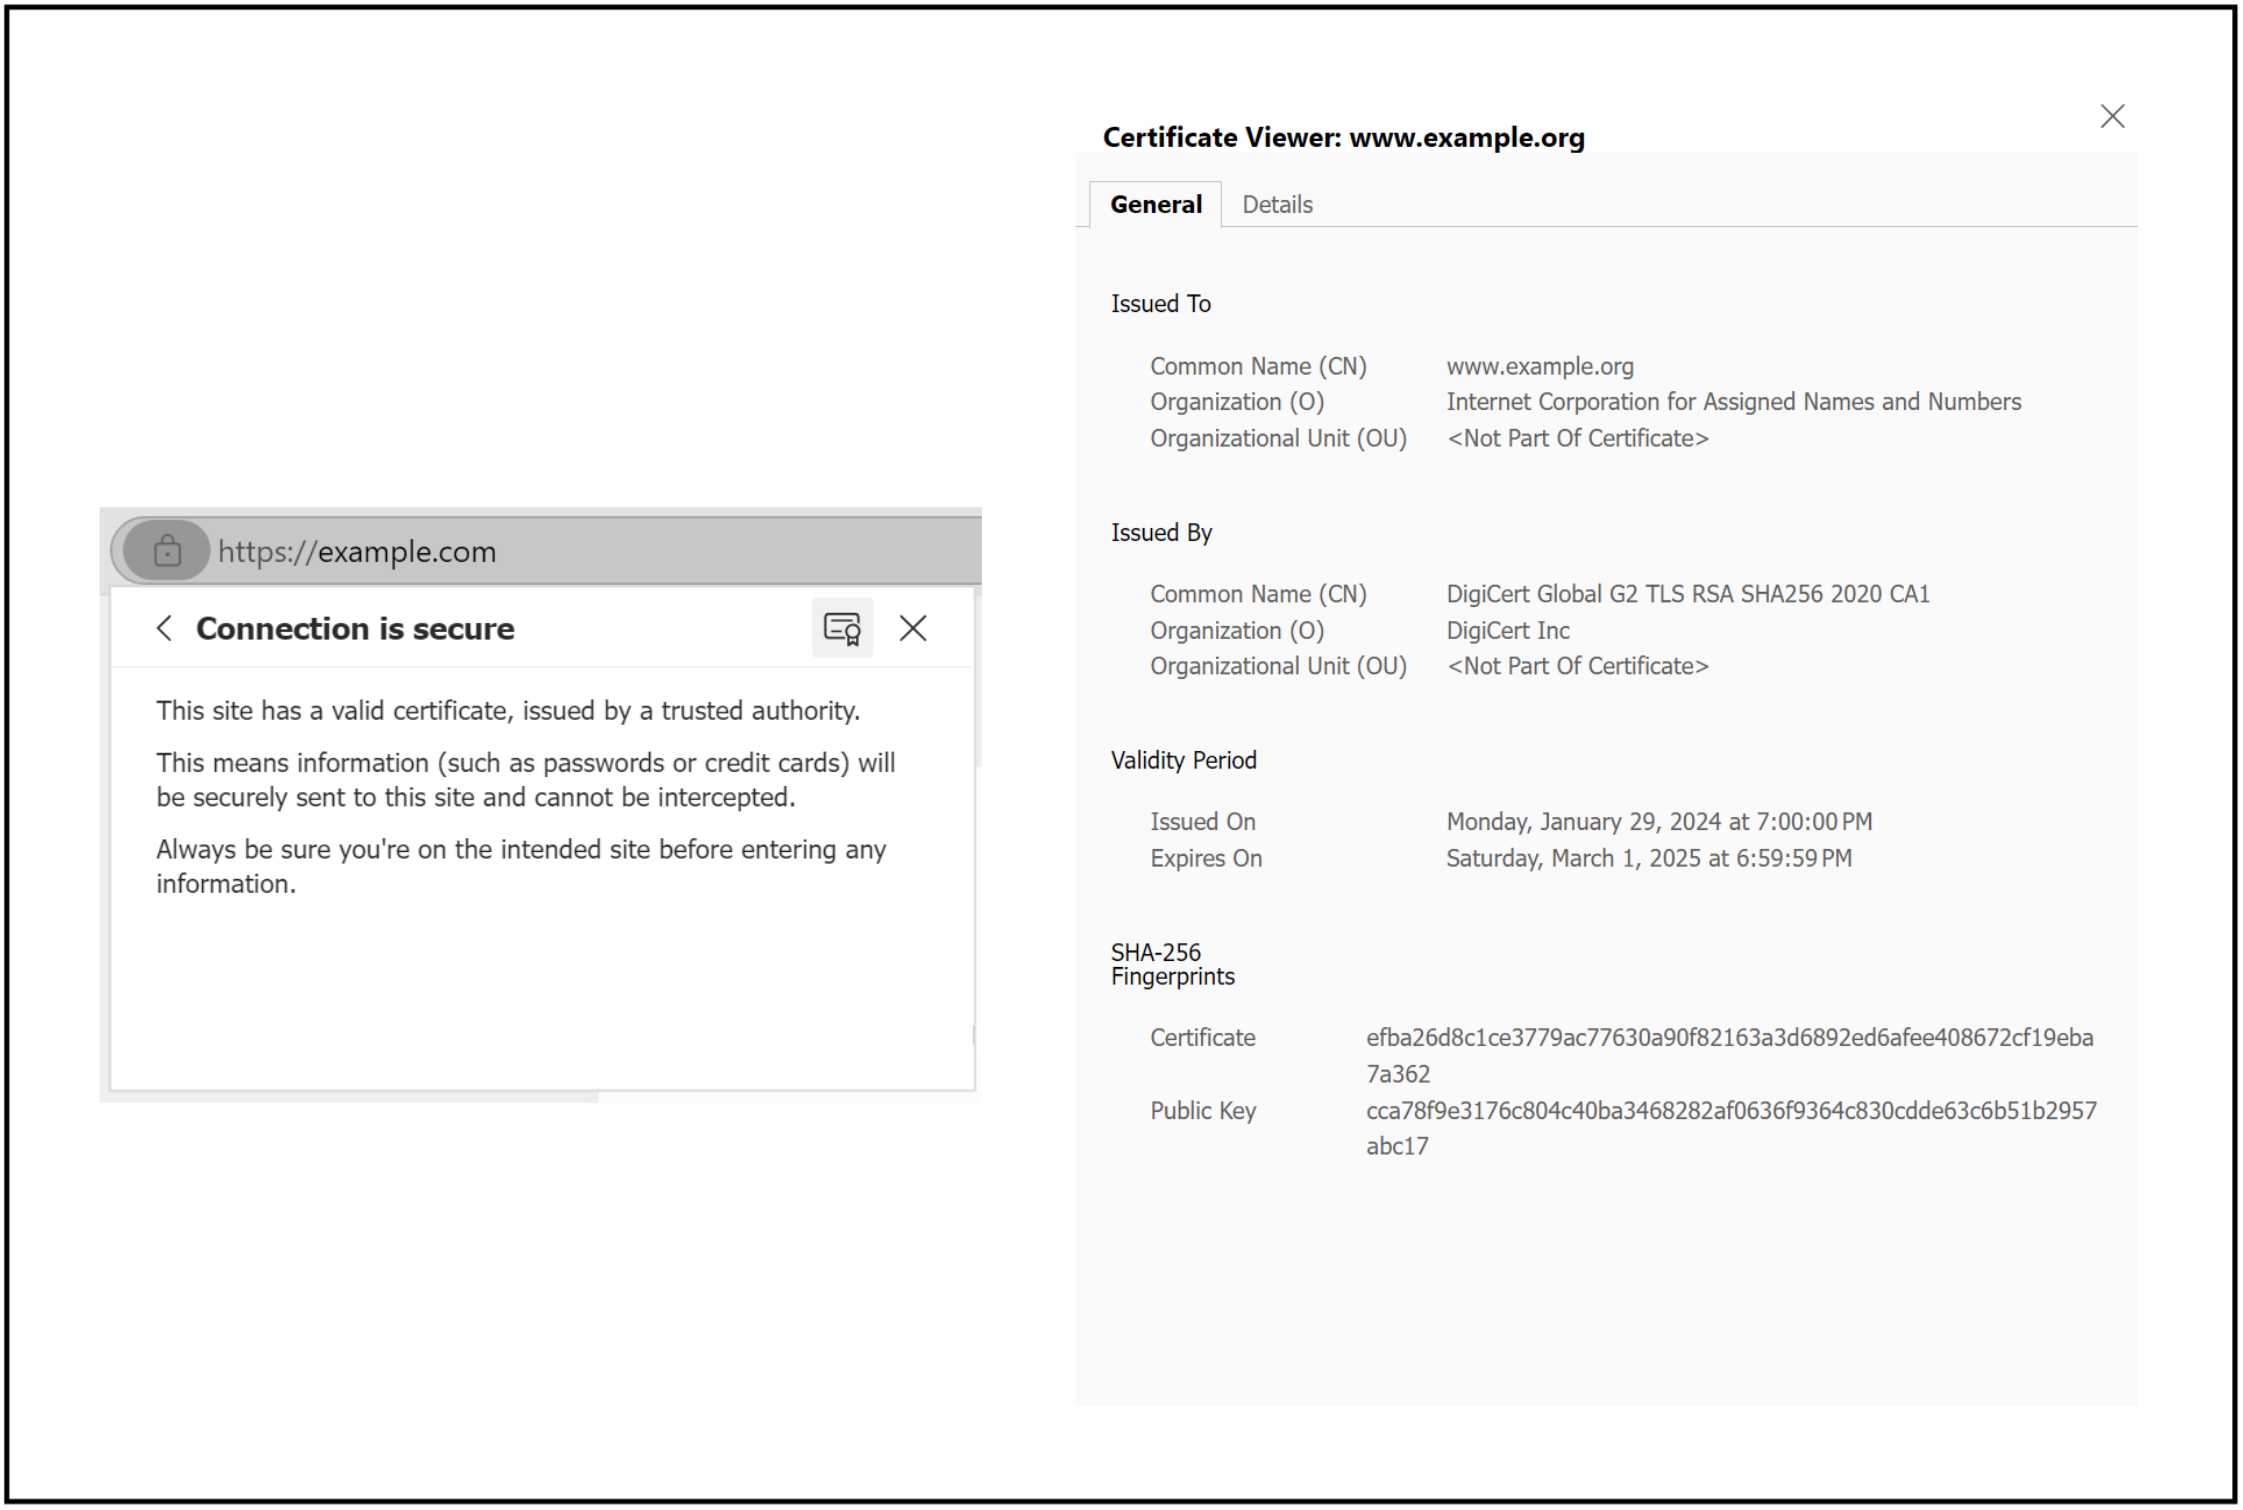
\includegraphics[width=1\textwidth]{Sections/sec/cert.png}
    \caption{SSL certificate obtained through the Edge browser on example.com}
    \label{fig:cert}
\end{figure}

\newpage 

\begin{Def}[Public Key Infrastructure (PKI)]

    PKI is a system for managing digital certificates. It includes the creation, distribution, and revocation of certificates.
    PKI is used to secure data transmission over the internet such as secure email, VPNs, and other services.
    \hfill \cite{okta_pki}
\end{Def}

\begin{Def}[Digtial \& Authority Certificates]

    \textbf{Digital Certificate}: An electronic document binding and proving ownership of a public key.\\
    \textbf{Authority Certificate}: or \textbf{Root Certificate} issued by a CA, signs other certificates.
    it is \textbf{self-signed} and is the top of the certificate chain.
    
    This establishes layers of trust and distance between the root certificate and the end-user certificates.
    If the root certificate is compromised, all certificates through the chain are compromised.
    \hfill \cite{yitzhak_digital_certificates}
\end{Def}

\begin{Def}[Digital Signatures]
    
    To verify a source, a \textbf{digital signature} is used. 
    \begin{itemize}
        \item \textbf{Key Generation}: A private and public key pair is generated beforehand.
        \item \textbf{Hashing}: A cryptographic hash of the data is created.
        \item \textbf{Encryption}: The private key encrypts the hash, creating the digital signature through an algorithm.
        \item \textbf{Verification}: The recipient decrypts the signature with the public key and compares the result to their own hash of the data. \hfill \cite{cisa_digital_signatures}
    \end{itemize}
\end{Def}

\begin{Def}[Certificate Signing Request (CSR)]

    To obtain a digital certificate, a client generates a CSR, which involves the following steps:
    \begin{enumerate}
        \item \textbf{Generate Key Pair}: Create a private key (kept secret) and a public key (shared).
        \item \textbf{Produce CSR Data}: Include identifying information (e.g., Organization (O), Common Name (CN)), the public key, and other details in a standardized format such as X.509.
        \item \textbf{Sign the CSR}: Hash the CSR data and sign it using the private key to prove ownership.
        \item \textbf{Submit and Issue Certificate}: Submit the CSR to a CA, which validates the signature, signs the certificate with its own private key, and issues the certificate.
        \hfill \cite{rfc2986}
    \end{enumerate}
\end{Def}


\begin{figure}[h!]
    \centering
    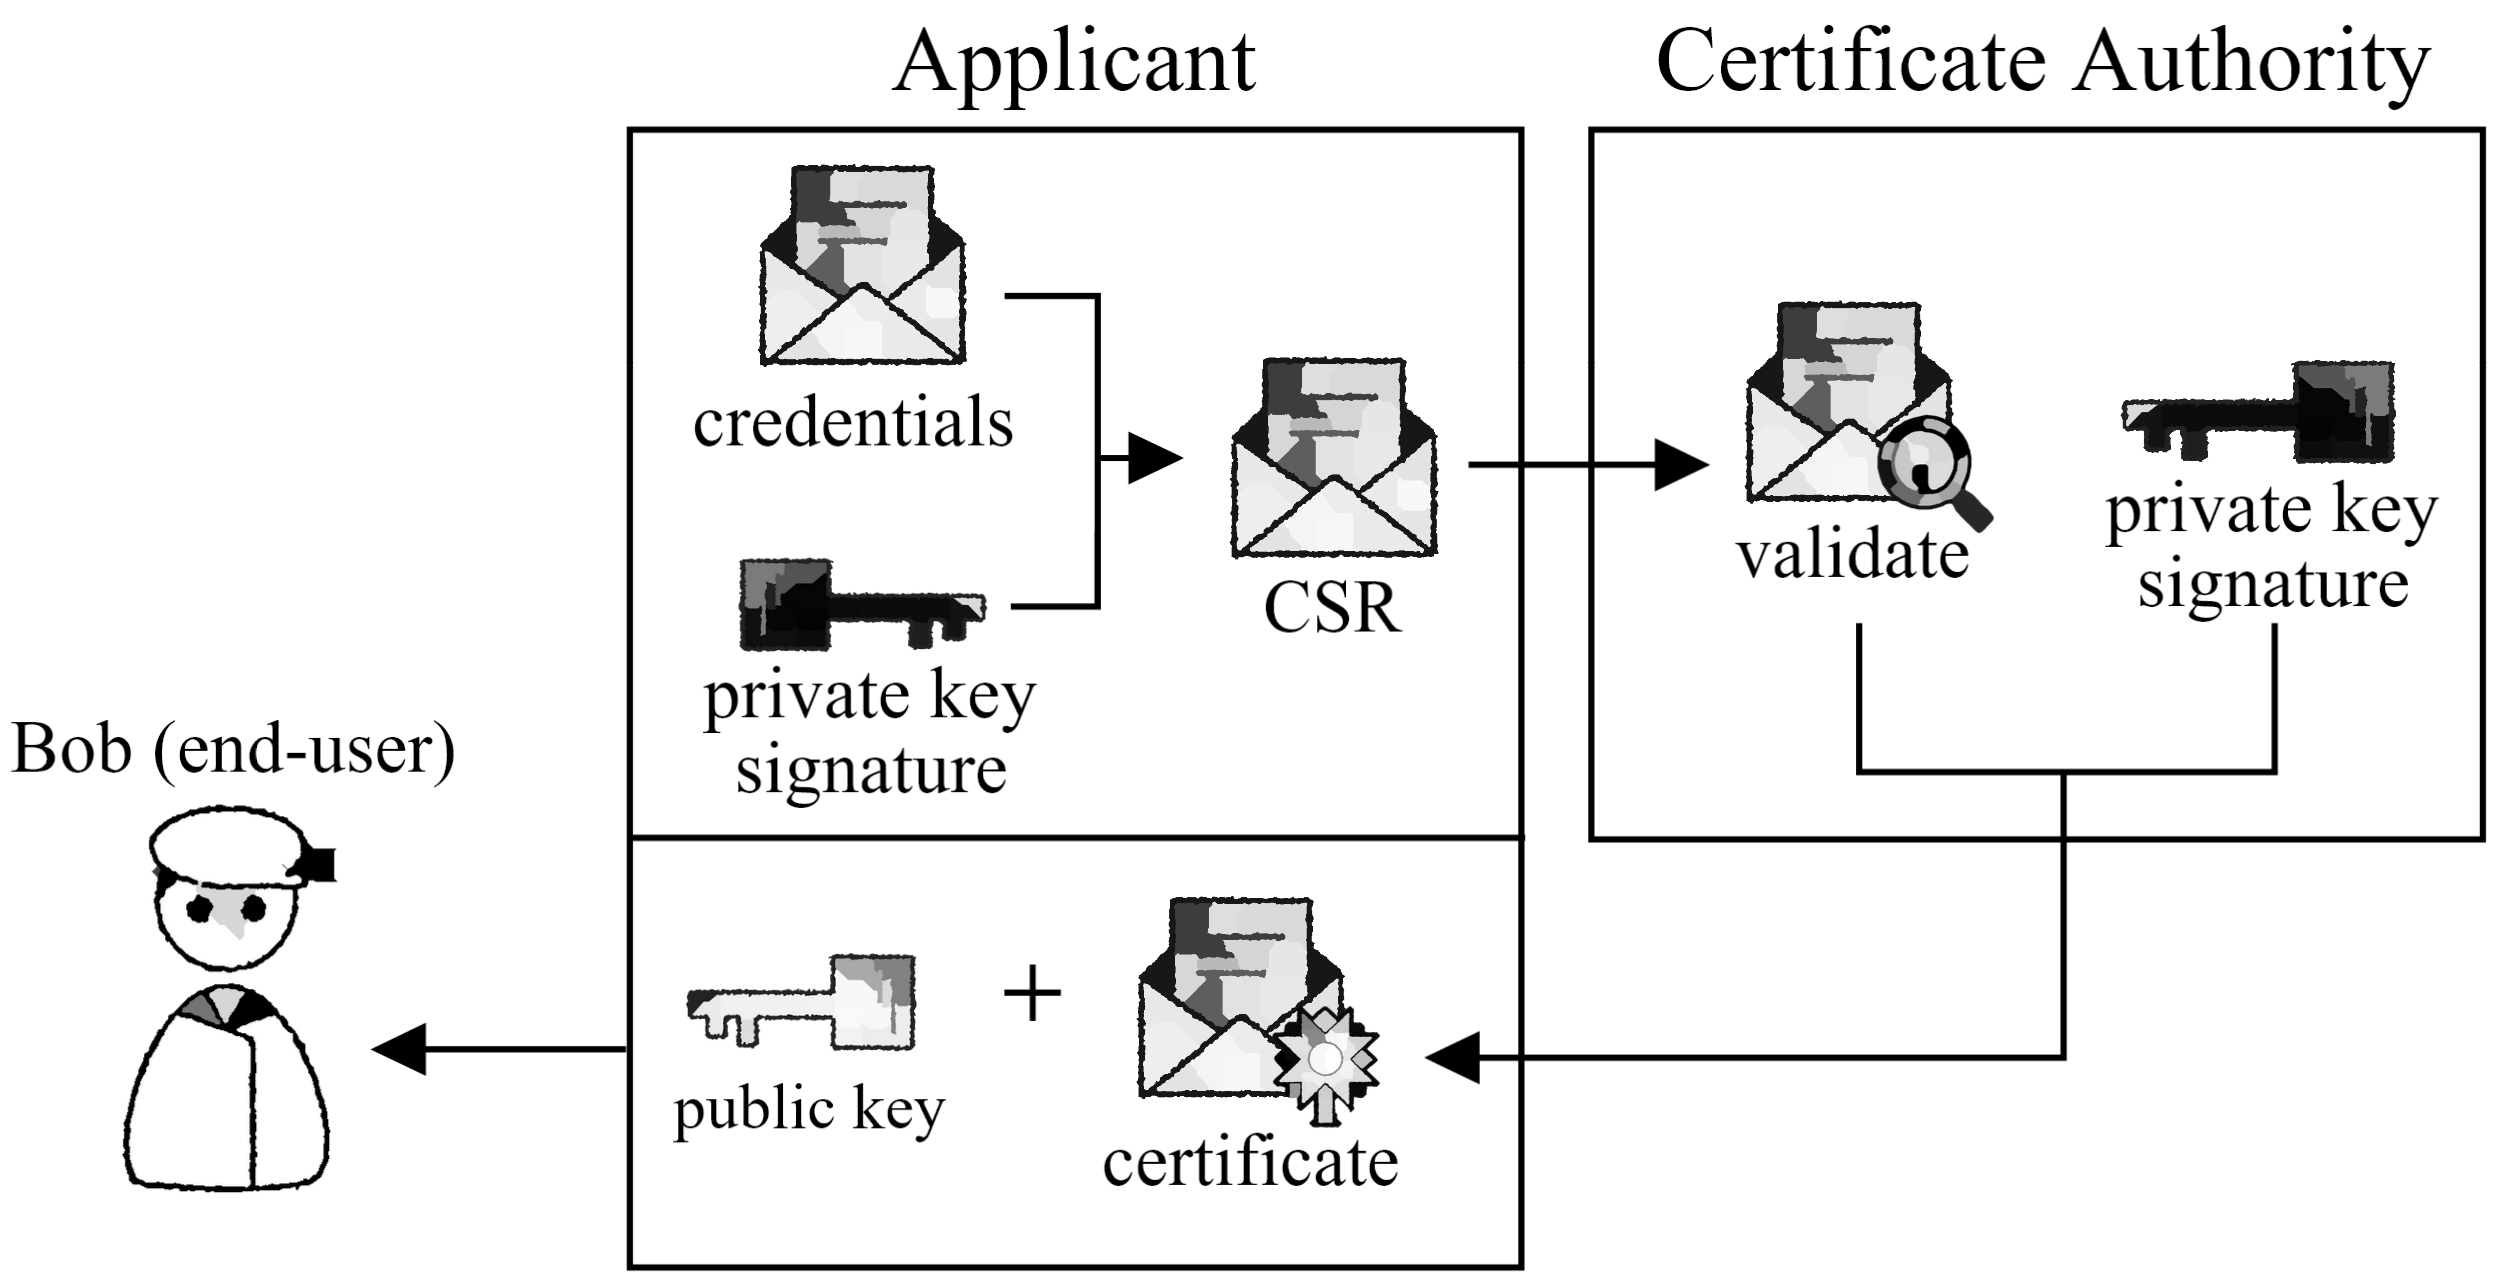
\includegraphics[width=1\textwidth]{Sections/sec/csr.png}
    \caption{Example of a Certificate Signing Request (CSR)}
    \label{fig:csr}
\end{figure}

\begin{Def}[Certificate Revocation List (CRL)]

    A CRL is a list of certificates that have been revoked by the CA before their expiration date.
    This is used to prevent the use of compromised certificates.
    \hfill \cite{rfc5280}
\end{Def}

\begin{Def}[Chain of Trust]

    A \textbf{Chain of Trust} is a hierarchical sequence of certificates used in PKI to establish trust between entities. It consists of:
    \begin{itemize}
        \item \textbf{Root Certificates}: Self-signed certificates at the top of the trust chain, trusted directly by operating systems and browsers.
        \item \textbf{Intermediate Certificates}: Issued by the root CA to delegate trust, adding a layer of security by isolating the root CA from direct interactions.
        \item \textbf{End-Entity Certificates}: Issued to users, servers, or devices to authenticate their identity and enable secure communications.
    \end{itemize}
    Each certificate is digitally signed by the private key of the certificate authority above it in the chain, with the root certificate serving as the ultimate trust anchor.
    Certified issuers are preferred over self-signed certificates because they undergo rigorous external validation, creating a verifiable path of trust. \hfill \cite{rfc5280}
\end{Def}

\newpage 

\begin{figure}[h!]
    \centering
    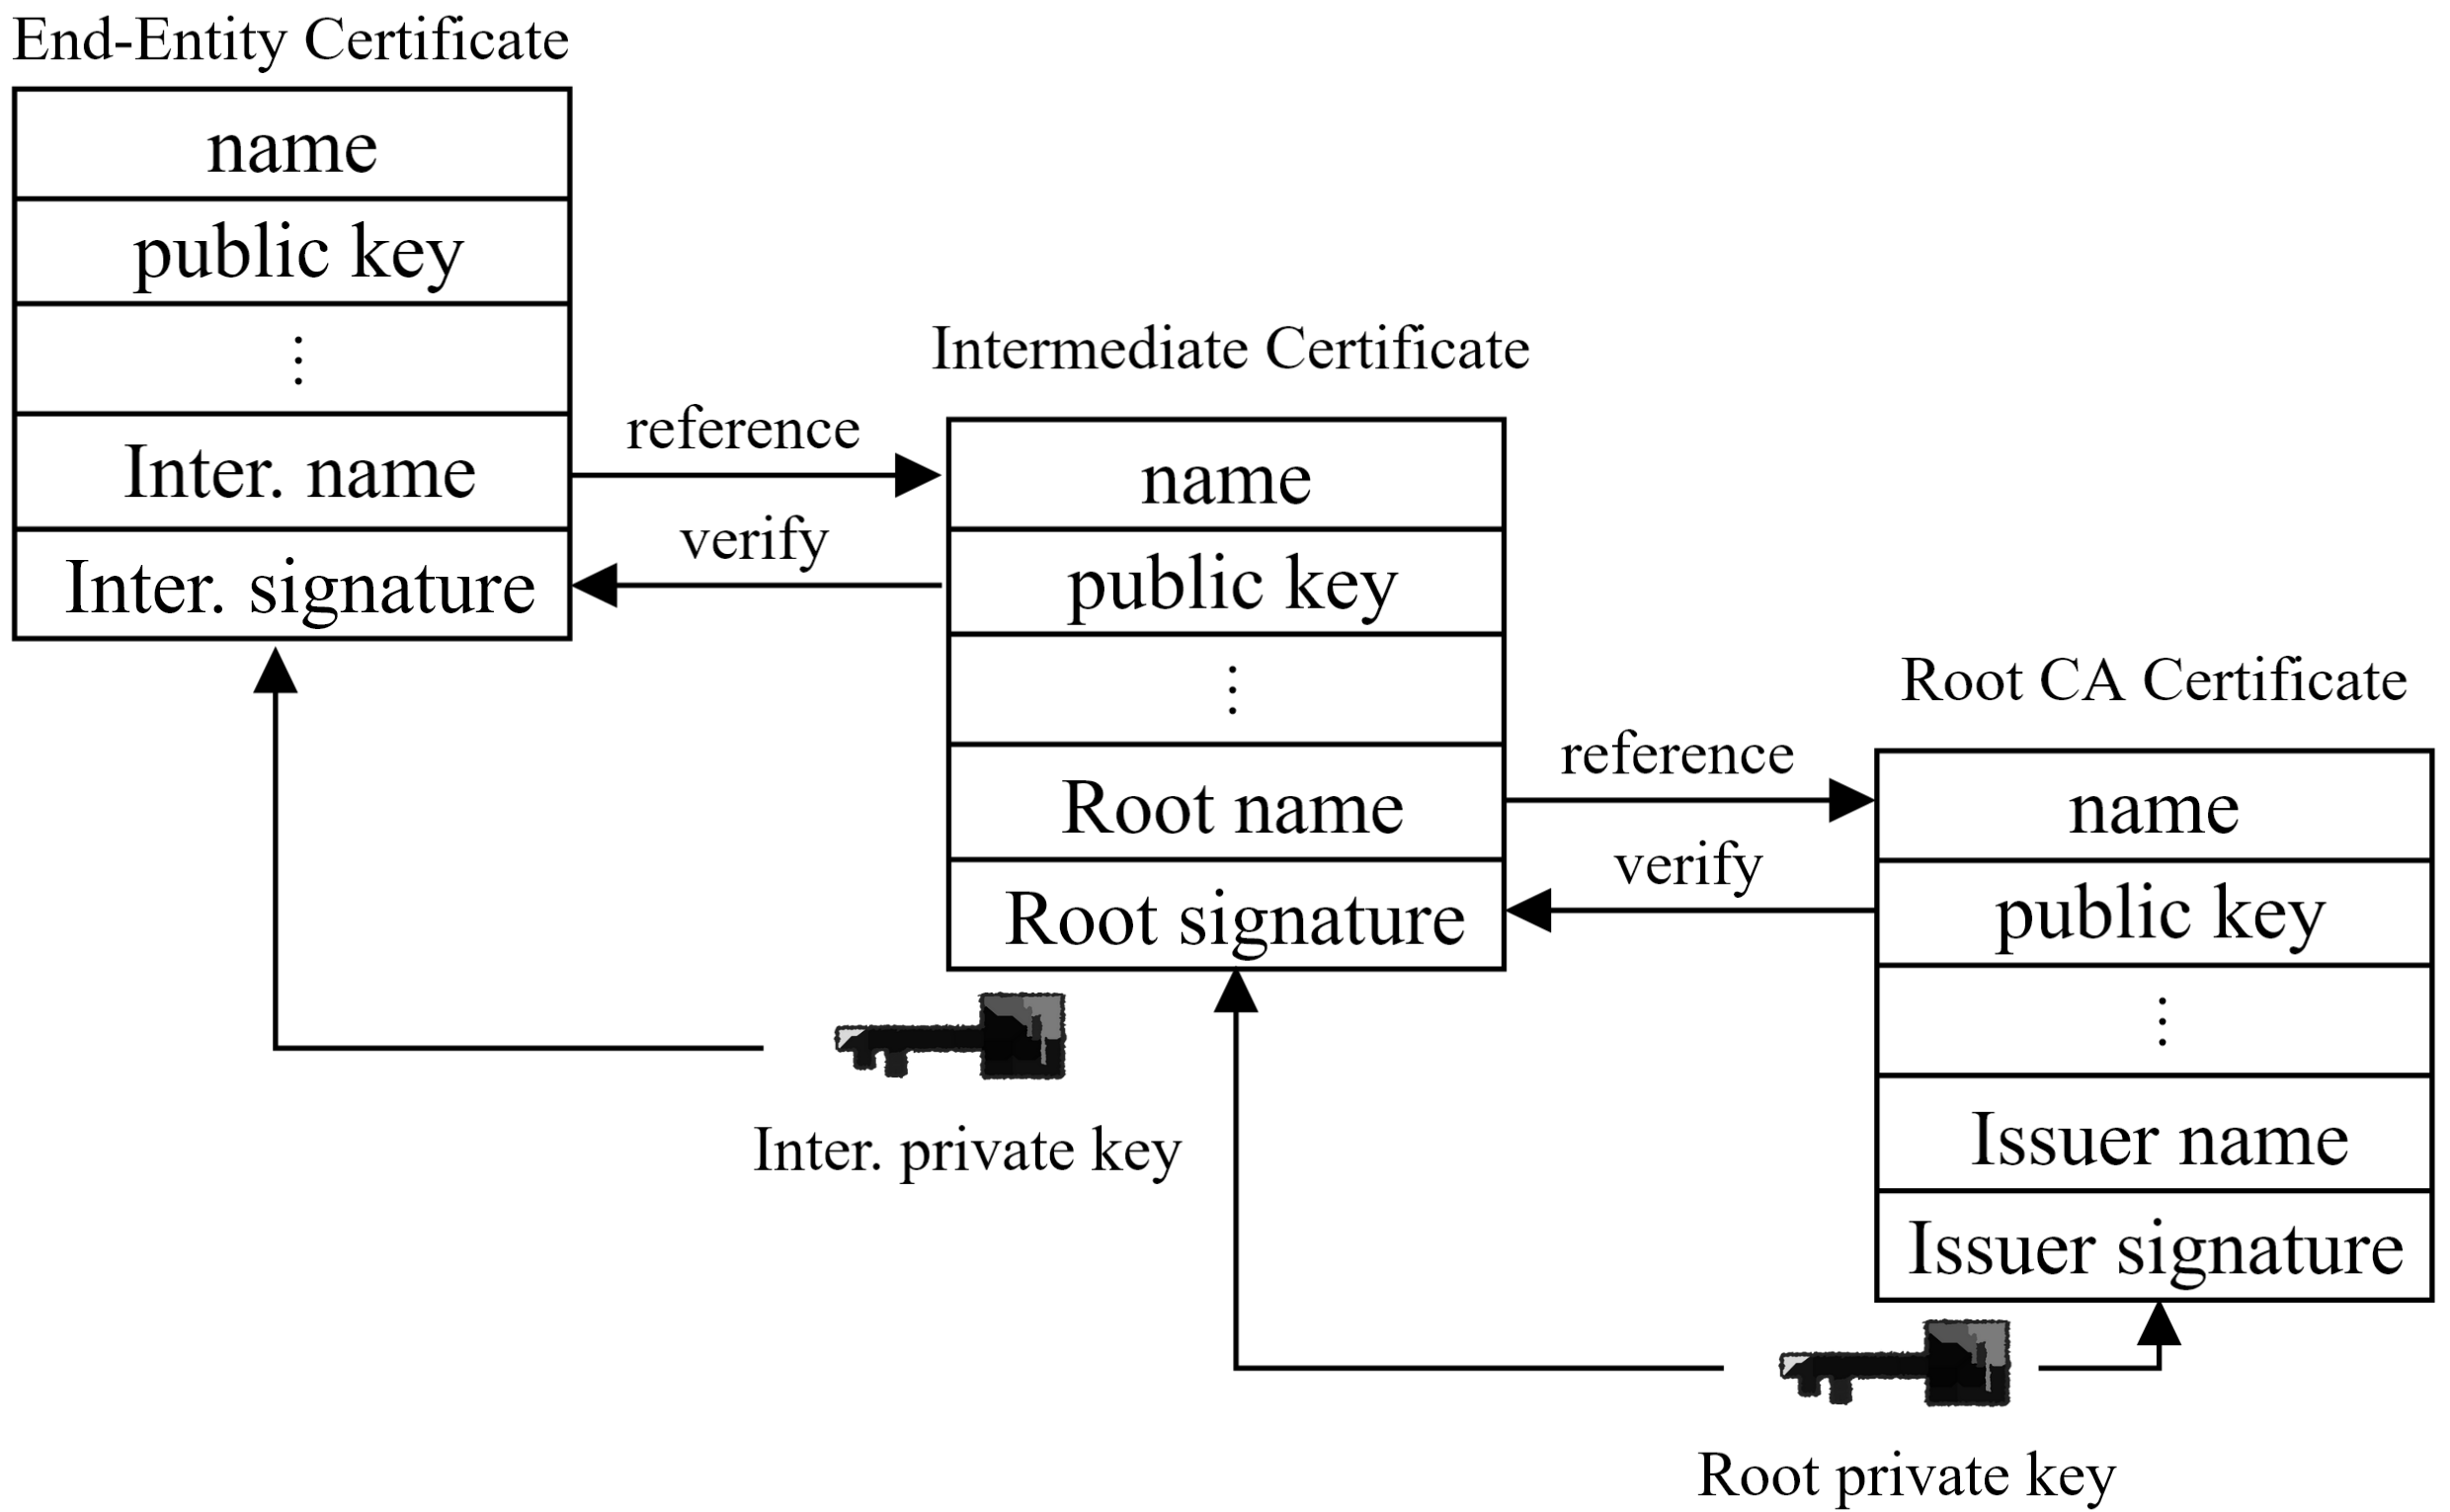
\includegraphics[width=1\textwidth]{Sections/sec/chain.png}
    \caption{A Chain of Trust from the Root Certificate to the End-Entity Certificate.}
    \label{fig:chain}
\end{figure}

\begin{Def}[Root Certificate Authority (CA) Signing Ceremonies]

    A \textbf{Root Certificate Authority (CA) Signing Ceremony} is a highly secure process in which a Root CA's private key is used to sign subordinate certificates, establishing trust within a Public Key Infrastructure (PKI). Key characteristics include:

    \begin{itemize}
        \item \textbf{Rigorous Security}: Conducted in offline, access-controlled environments with multiple layers of physical and procedural security. Entry requires the presence of multiple trusted individuals simultaneously.
        \item \textbf{Defined Roles}: Roles such as Crypto Officers, Witnesses, and Administrators are assigned to ensure transparency and accountability.
        \item \textbf{Global Trust Anchors}: Managed by organizations like ICANN for DNSSEC, these ceremonies protect the integrity of critical internet infrastructure.
        \item \textbf{Independent Operations}: Root CAs are typically independent from government oversight, though some, like the
        U.S. Department of Defense, manage government-affiliated Root CAs. 
    \end{itemize}
    Learn More: \href{https://www.cloudflare.com/learning/dns/dnssec/root-signing-ceremony/#:~:text=That%E2%80%99s%20the%20purpose%20of%20the%20Root%20Signing%20Ceremony%E2%80%94a,literally%20the%20key%20to%20the%20entire%20DNSSEC-protected%20Internet.}{https://cloudflare.com/learning/dns/dnssec/root-signing-ceremony/} \hfill \cite{cloudflare_root_signing}
\end{Def}

\newpage 

\noindent
\begin{Def}[DNS over HTTPS (DoH) and DNS over TLS (DoT)]

    \textbf{DNS over HTTPS (DoH)} and \textbf{DNS over TLS (DoT)} are protocols designed to encrypt DNS queries, improving privacy and security:
    \begin{itemize}
        \item \textbf{DoH}: Encrypts DNS queries over the HTTPS protocol (port 443), making them indistinguishable from regular HTTPS traffic.
        \item \textbf{DoT}: Encrypts DNS queries using the TLS protocol (port 853), ensuring DNS requests are secure and tamper-proof.
        Though because of its use of port 853, traffic is more easily identifiable as DNS, making DoH the preferred method.
    \end{itemize}

    \noindent
    DNS security is known as \textbf{DNSSEC}. \hfill \cite{cloudflare_dns_tls}
\end{Def}














\section{Encryption Algorithms \& Security Definitions}
\label{sec:enc}
\noindent
In the previous section the notion of encryption was introduced (asymmetric and symmetric).
Here adversaries (i.e., attackers, or hackers) will be defined along with the specifications an algorithm must meet.

\begin{Def}[Adversaries]

    \label{def:adversaries}
    Adversaries are entities that attempt to break the security of a system.
    There are two types of adversaries:
    \begin{itemize}
        \item \textbf{Eavesdroppers:} Can only intercept and read messages.
        \item \textbf{Man-in-the-Middle (MitM):} Can intercept, read, and modify messages.
    \end{itemize}
\end{Def}

\begin{figure}[h!]
    \centering
    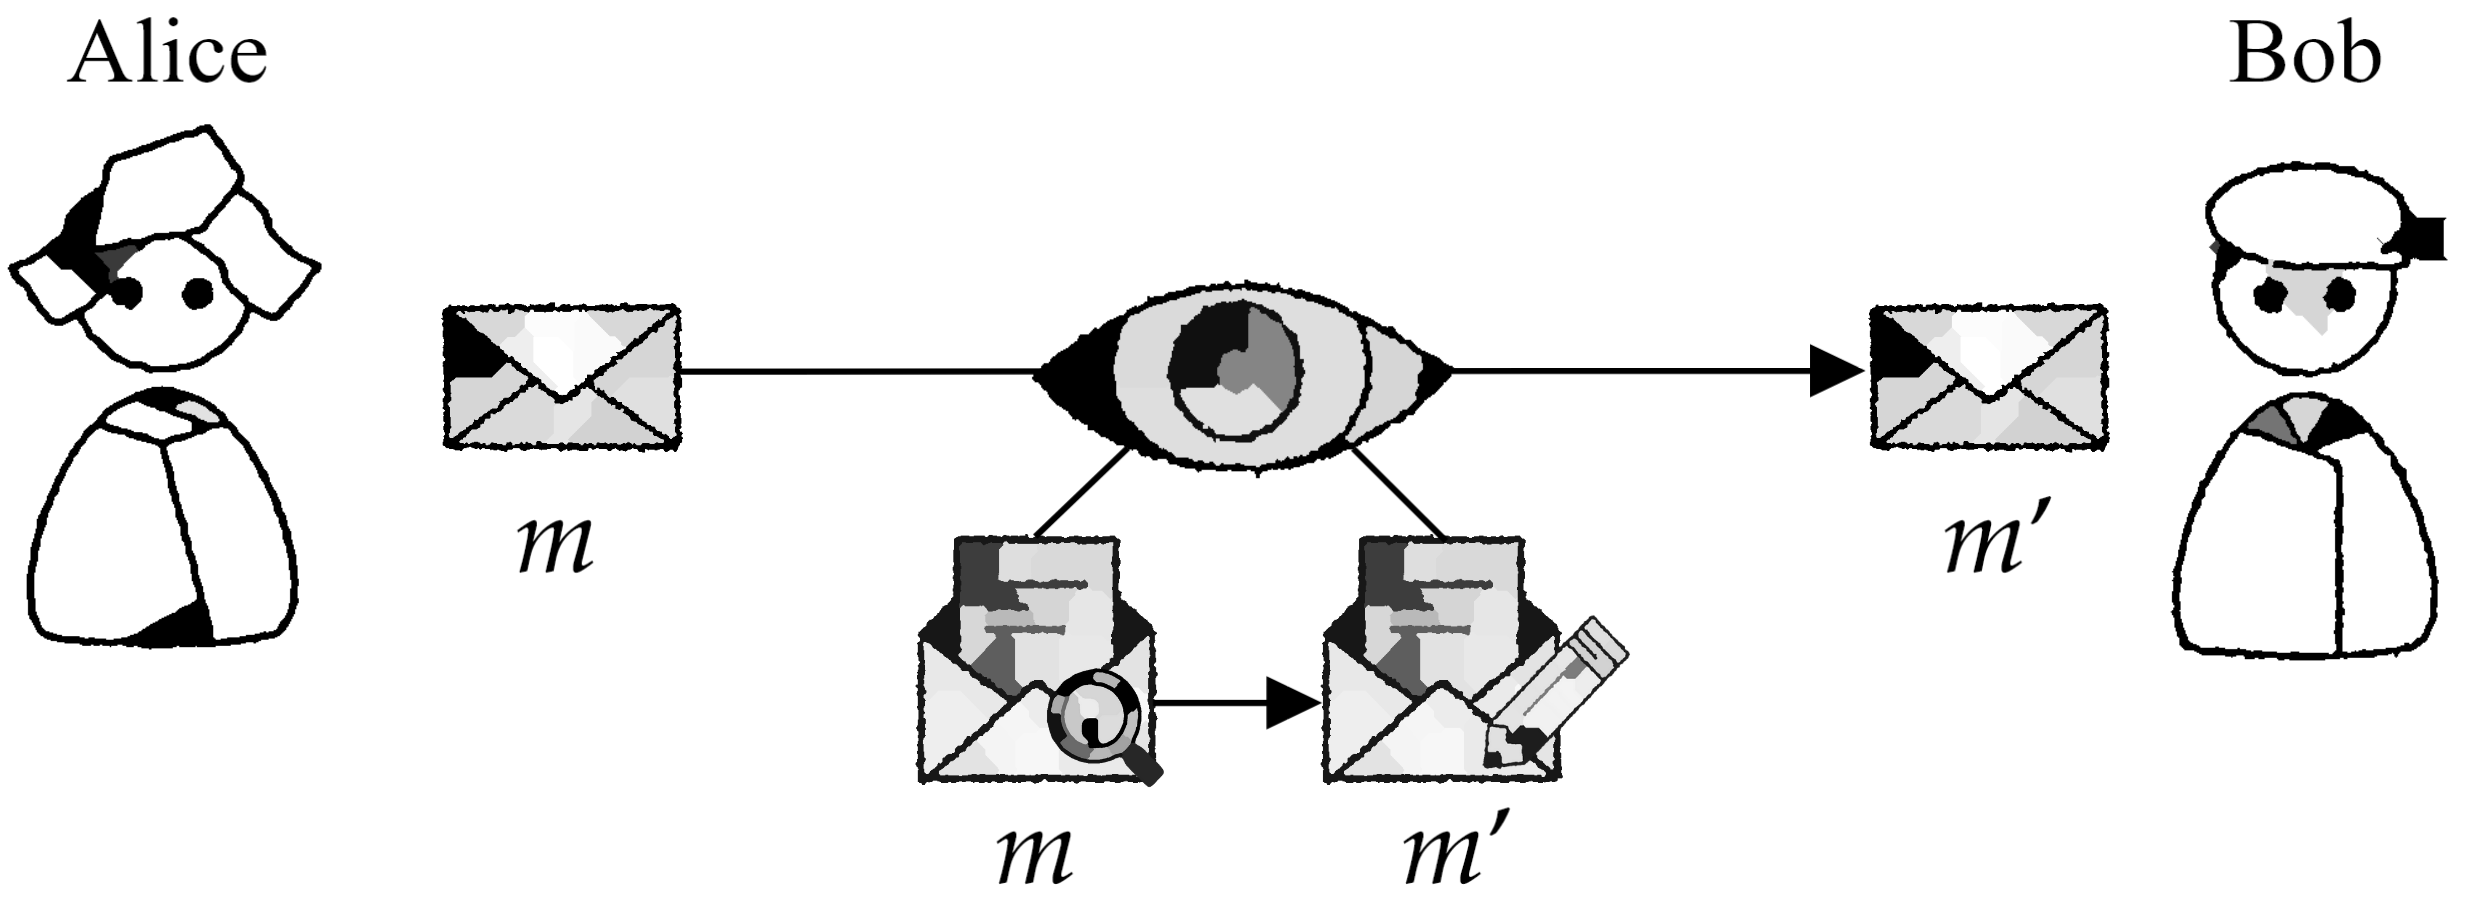
\includegraphics[width=.8\textwidth]{Sections/sec/enc/mitm.png}
    \caption{A MitM Attack, reading and altering the contents of $m$ and sending $m'$.}
    \label{fig:adv}
\end{figure}

\noindent
Instead plain variables $A$ and $B$, often Alice and Bob are used. There are other common for entities, learn more here:
\href{https://en.wikipedia.org/wiki/Alice_and_Bob}{https://en.wikipedia.org/wiki/Alice\_and\_Bob}.

\newpage 
\begin{Def}[Security Definitions]

    \label{def:security_definitions}
    Security definitions formalize the properties a system must satisfy to resist adversarial attacks. These include:
    \begin{itemize}
        \item \textbf{Confidentiality:} Ensures that adversaries cannot learn the contents of the message.
        \item \textbf{Integrity:} Guarantees that adversaries cannot alter the message without detection.
        \item \textbf{Authenticity:} Verifies that the message originates from the claimed sender and has not been tampered with.
    \end{itemize}
\end{Def}

\begin{theo}[Kerckhoffs's Principle]

    \label{theo:kerckhoffs}
    \begin{center}
        \Large\textit{``Il faut qu'il n'exige pas le secret, et qu'il puisse sans inconvénient tomber entre
        les mains de l'ennemi.''}
    \end{center}

    \vspace{1em}
    \normalsize

    \noindent
    \textbf{Literal translation}: [The method] must not be required to be secret, and it
    must be able to fall into the enemy's hands without causing inconvenience \cite{joyofcryptography}.
\end{theo}

\begin{figure}[h!]
    \centering
    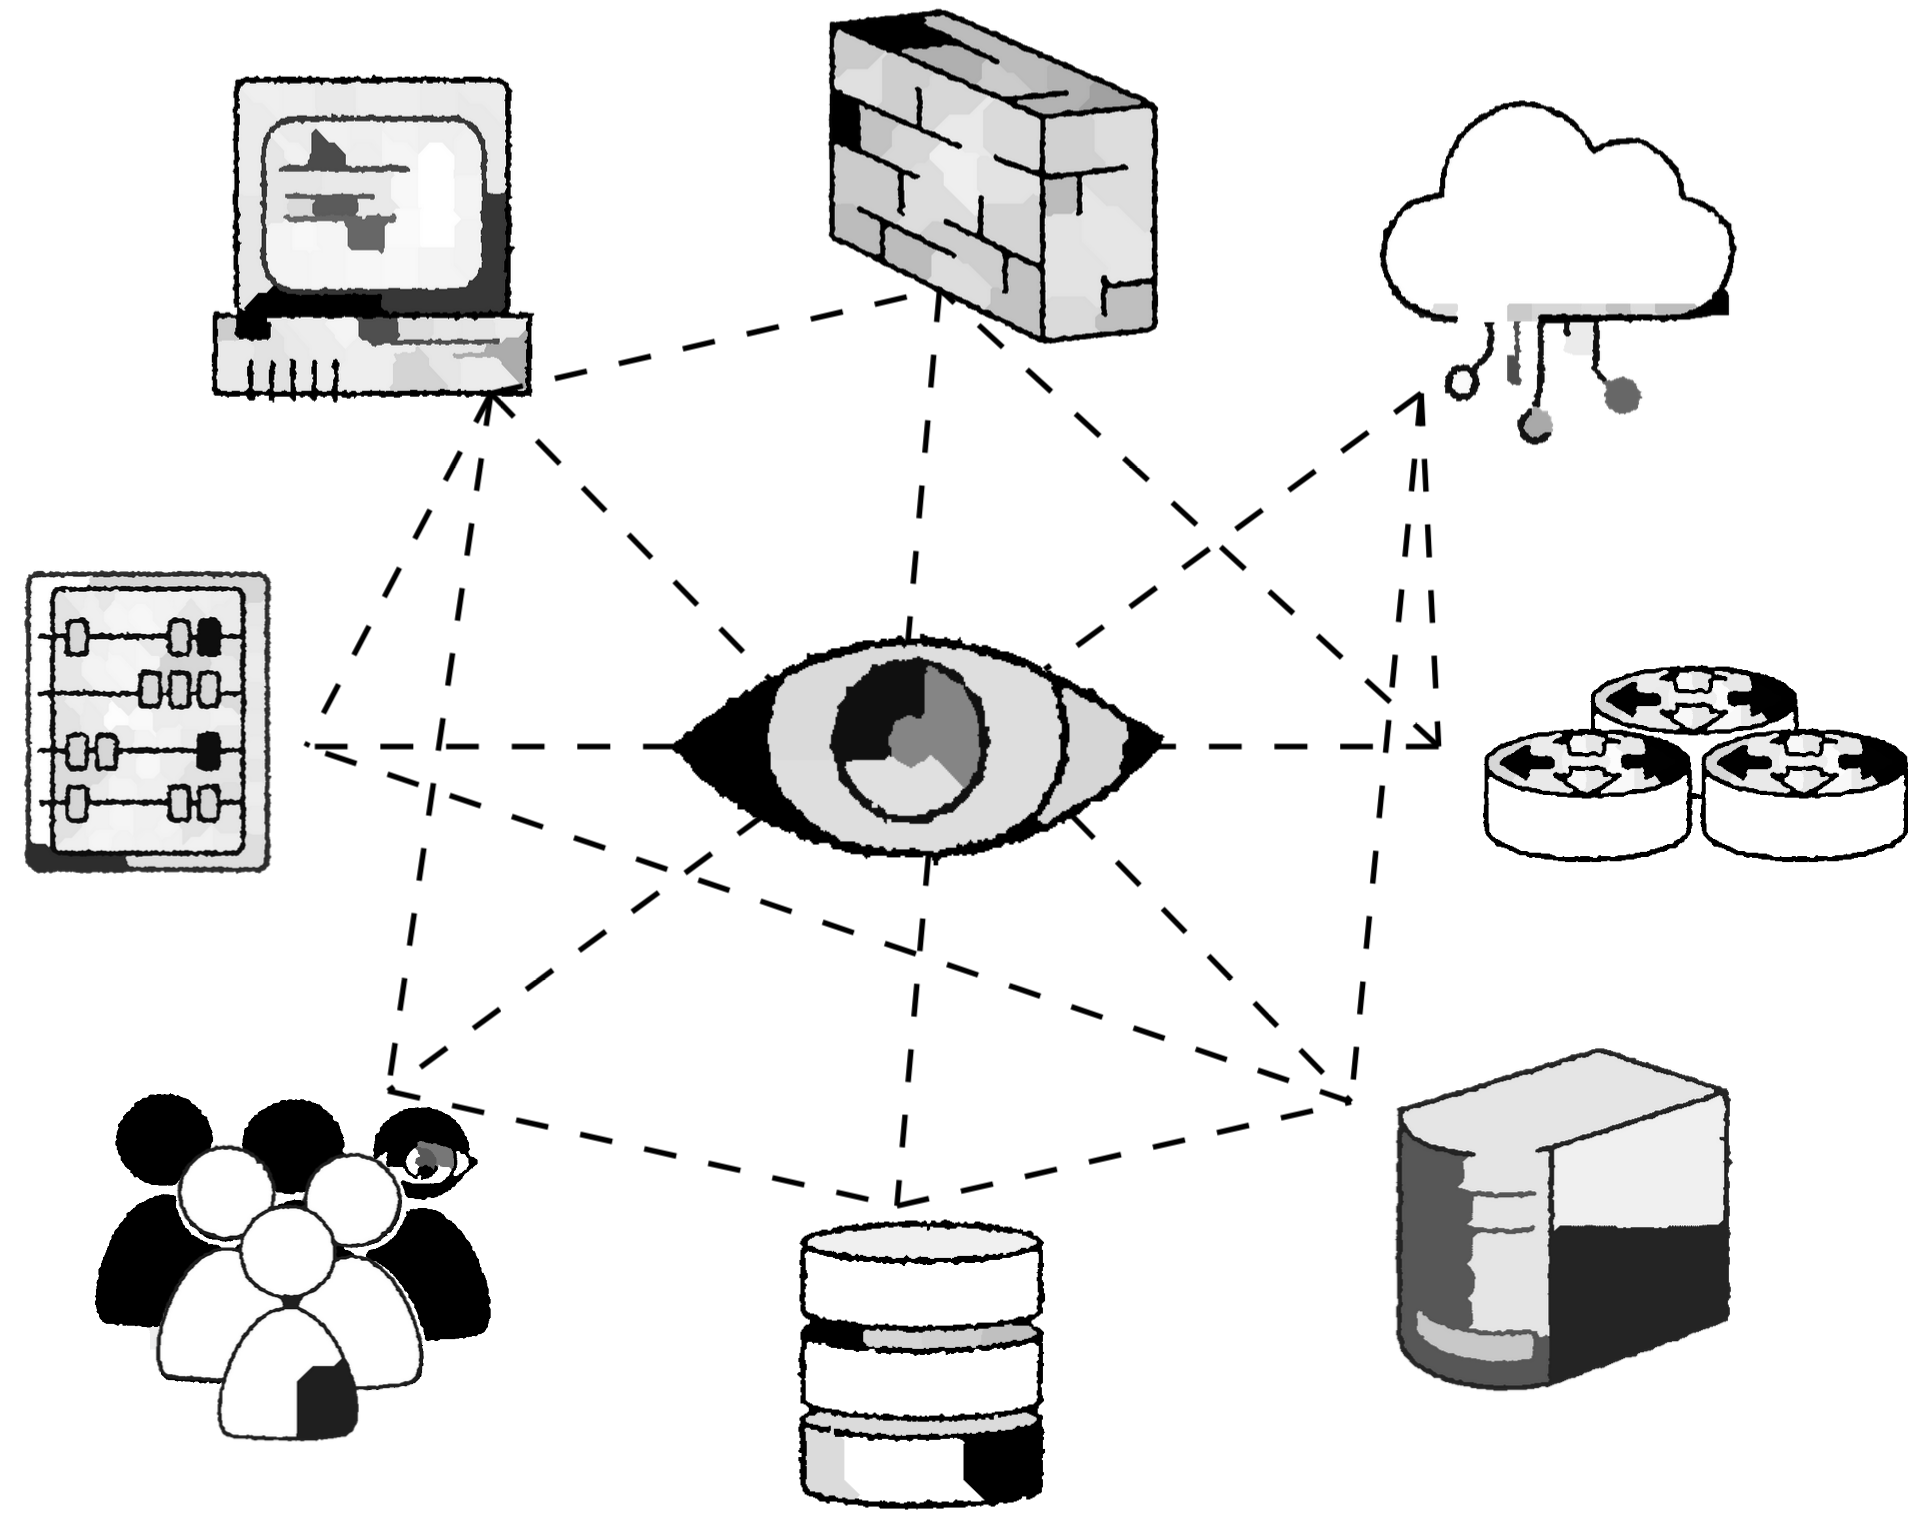
\includegraphics[width=.6\textwidth]{Sections/sec/enc/enemy.png}
    \caption{Kerckhoffs's Principle, an adversary's unbounded sight.}
    \label{fig:kerckhoffs}
\end{figure}

\noindent
I.e., \textbf{The adversary knows all}---the algorithm, the architecture, an insider, any exploit---all communication is naked, visible on the wire.
Though despite all, is secure. This is the essence of Kerckhoffs's Principle.

\newpage

\begin{Def}[Non-cryptographic Security]

    \label{def:non_crypto}
    A system which does not follow Kerkhoff's Principle: security through obscurity (hiding the algorithm) is not a cryptographic. As 
    if any rosetta stone is found, the system is compromised.
\end{Def}

\vspace{-1em}
\begin{Note}
    \textbf{Note}: The rosetta stone was a slab of stone found in 1799, which helped decipher Egyptian hieroglyphics. I.e., a key between languages.
    Learn more: \href{https://en.wikipedia.org/wiki/Rosetta_Stone}{https://wikipedia.org/rosetta\_stone}.
\end{Note}

\noindent
The rest of the section will cover methods used over centuries to attempt to secure messages.

\begin{theo}[Caesar Cipher]

    \label{theo:caesar_cipher}
    The Caesar Cipher is a non-cryptographic scheme, named after Julius Caesar, dating back 45BC to protect military communications.
    Each letter in the plaintext is shifted $x$ places down the alphabet. E.g., $x= 3$, `A'=`D', `B'=`E', and so on. \hfill \cite{timour2019crypto}
\end{theo}

\vspace{-1em}
\begin{Note}
    \textbf{Note}: Here is a fun online tool to try the Caesar Cipher: \href{https://cryptii.com/pipes/caesar-cipher}{https://cryptii.com/caesar-cipher}.
\end{Note}

\begin{theo}[Vigenère Cipher]

    \label{theo:vigenere_cipher}
    The Vigenère Cipher is a non-cryptographic scheme, created in mid-1500's by italian cytologist Giovan Battista Bellaso,
    later popularized and misattributed to Blaise de Vigenère. It addressed the Caesar Cipher's weakness by using attributing odd and even digit places to different Caesar Ciphers.

    This was aimed to stop frequency analysis attacks, as for instance, `E' is the most common letter in English. If a letter is repeated at high frequency, it is likely `E'. \hfill \cite{timour2019crypto}
\end{theo}
\begin{figure}[h!]
    \centering
    \[
    \begin{array}{c|c|c|c|c|c|c|c|c|c|c|c|c|c|c|c|c|c|c|c|c|c|c|c|c|c|c}
    
    0 & a & b & c & d & e & f & g & h & i & j & k & l & m & n & o & p & q & r & s & t & u & v & w & x & y & z \\ \hline\hline
    1 & f & g & h & i & j & k & l & m & n & o & p & q & r & s & t & u & v & w & x & y & z & a & b & c & d & e \\ \hline
    2 & k & l & m & n & o & p & q & r & s & t & u & v & w & x & y & z & a & b & c & d & e & f & g & h & i & j \\
    \end{array}
    \]
    \caption{Vigenère Cipher Table: row 0 is the key, 1 even, and 2 odd shift.}
    \label{fig:caesar_shift_table}
\end{figure}

\noindent
For example ``Coffee'' would be ``hykpjo'' deterring frequency analysis of the letter `E'.

\newpage 

\begin{Func}[Key \& String Length ($\lambda,\|a\|$)]

    \vspace{-.5em}
    \label{func:bit_length}
    The rest of the text may denote `$\lambda$' (lambda) as the bit length of the key. E.g., $\lambda = 8$ bits, which in in binary may hold $2^8 = 256$ values ($[0000\ 0000]_2\text{-}[1111\ 1111]_2$).
    The $\lambda$ is variable is often called the \textbf{security parameter}.\\
    \noindent
    \rule{\textwidth}{0.4pt}
    \textbf{For ease of notation}, $\|a\|$ denotes the length of a character or binary string $a$. E.g., $\|a\| = 5$ for the string $a = \text{``hello''}$
    (the use of which will always be explicit).
    \hfill \cite{joyofcryptography}
\end{Func}

\begin{Def}[One-Time Pad (OTP)]

    \label{def:one_time_pad}
    OTP, also known as the \textbf{Vernam Cipher} is a cryptographic scheme, invented by Gilbert Vernam in 1919.
    Earlier depictions though date back to 1882 by Frank Miller on telegraphy.\\
    \noindent
    \rule{\textwidth}{0.4pt}
    \textbf{Security Definition}: Confidentiality is guaranteed if the key is used only once.
\end{Def}

\begin{Func}[One Time Pad - \texttt{Enc(m, k)} \& \texttt{Dec(k, c)}]

    \vspace{-.5em}
    \label{func:otp}
    \noindent
    Let function $k\leftarrow\{0,1\}^{\lambda}$ generate keys $k$:
    \begin{itemize}
        \item $\{0,1\}$ denotes the set of possible inputs.
        \item $k$ is a random bit string of length $\lambda$ bits consisting of 0's and 1's. E.g., $\lambda = 8$ then $k = [1010\ 1101]_2$ is a possible output.
        \item $\{0,1\}^{\lambda}$ should be a uniform distribution, i.e., each bit is equally likely to be 0 or 1.
    \end{itemize}
    \noindent
    Let $m$ be and $c$ be an encrypted message, both length $\lambda$ bits. Then: 
    \begin{itemize}
        \item $c\leftarrow \text{Enc}(m,k) := m\oplus k$. (Encryption)
        \item $m\leftarrow \text{Dec}(k,c) := c\oplus k$. (Decryption)
    \end{itemize}

    \noindent
    Where $\oplus$ denotes the XOR operation $(1\oplus1=0; 0\oplus1=1; 1\oplus0=1; 0\oplus0=0)$.
\end{Func}

\[
c\gets\text{Enc}(m,k) :=
\begin{cases}
\begin{array}{r@{\;}r}
\textcolor{Wine}{0011\ 0100\ 1101\ 1000\ 1111} & \hspace{1em} (m) \\[2pt]
\oplus\ \textcolor{Wine}{1110\ 1010\ 0110\ 1000\ 1101} & \hspace{1em} (k) \\[2pt]
\hline
\textcolor{Wine}{1101\ 1110\ 1011\ 0000\ 0010} & \hspace{1em} (c)
\end{array}
\end{cases}
\text{(Encryption)}
\]
\[
m \gets \text{Dec}(c,k) :=
\begin{cases}
\begin{array}{r@{\;}r}
\textcolor{Wine}{1101\ 1110\ 1011\ 0000\ 0010} & \hspace{1em} (c) \\[2pt]
\oplus\ \textcolor{Wine}{1110\ 1010\ 0110\ 1000\ 1101} & \hspace{1em} (k) \\[2pt]
\hline
\textcolor{Wine}{0011\ 0100\ 1101\ 1000\ 1111} & \hspace{1em} (m)
\end{array}
\end{cases}
\text{(Decryption)}
\]
\newpage 

\noindent
The larger the key, the more secure the scheme becomes, as smaller keys have a higher probability of being brute-forced by generating
all possible keys.

\begin{theo}[Computational Security]

    \label{theo:computational_security}
    \textbf{Computational Security} is a security definition that guarantees that the adversary cannot break the scheme in a reasonable amount of time.
    In todays standards, exponential time algorithms are considered infeasible, (e.g., $O(2^{\lambda})$ time complexity).
\end{theo}

\vspace{-2em}
\begin{figure}[h!]
    \centering
    \[
    \begin{tabular}{ll}
        \textbf{Efficient algorithm known:} & \textbf{No known efficient algorithm:} \\
        Computing GCDs & Factoring integers \\
        Arithmetic mod \( N \) & Computing \( \phi(N) \) given \( N \) \\
        Inverses mod \( N \) & Discrete logarithm \\
        Exponentiation mod \( N \) & Square roots mod composite \( N \)
    \end{tabular}
    \]
    \caption{Comparison of problems with known efficient algorithms and those without \cite{joyofcryptography}.}
    \label{fig:efficient_vs_no_algorithm}
\end{figure}

\begin{Def}[Known \& Chosen Plaintext Attacks]

    \textbf{Known Plaintext Attack (KPA)}:\\
    The adversary has access to one or more known unencrypted and encrpyted message pairs.\\

    \vspace{-.5em}
    \noindent
    \textbf{Chosen Plaintext Attack (CPA)}:\\
    The adversary encrypts plaintext of their choosing to analyze the corresponding ciphertexts.
\end{Def}

\noindent
The Caesar Cipher and Vigenère Cipher are both vulnerable to plaintext attacks. The One-Time Pad (OTP), becomes vulnerable if the key is small or reused.


\begin{Def}[Block Ciphers]

    \label{theo:block_cipher}
    A cryptographic scheme that separates and encrypts fixed-length blocks of plaintext into ciphertext. Let $\beta$ (beta) be the block size, and $\lambda$ the key length.
    Then for a set of $B$ blocks and message $M$: $\sum_{b\in B} \beta = \|M\|$ (the sum of all blocks equals the length of the message).\\
    We define $\text{Enc}_\lambda(M,\beta)$, $\text{Dec}_\lambda(C,\beta)$, $C$ as the set of ciphertext blocks, s.t.:
    \begin{align*}
        \text{Enc}_\lambda(M,\beta) \rightarrow C : b\in B \mapsto c\in C\\
        \text{Dec}_\lambda(C,\beta) \rightarrow M : c\in C \mapsto b\in B\\
    \end{align*} 

    \vspace{-1em}
    \noindent
    Where $\lambda :=\{(b,c),\dots\}, \text{a dictionary of unique message block to ciphertext pairs (bijection)}$.
\end{Def}

\newpage 

\noindent
The below figure demonstrates use of a block cipher with a block size of 2, using the Electronic Codebook Mode (ECB).
\begin{figure}[h!]
    \centering
    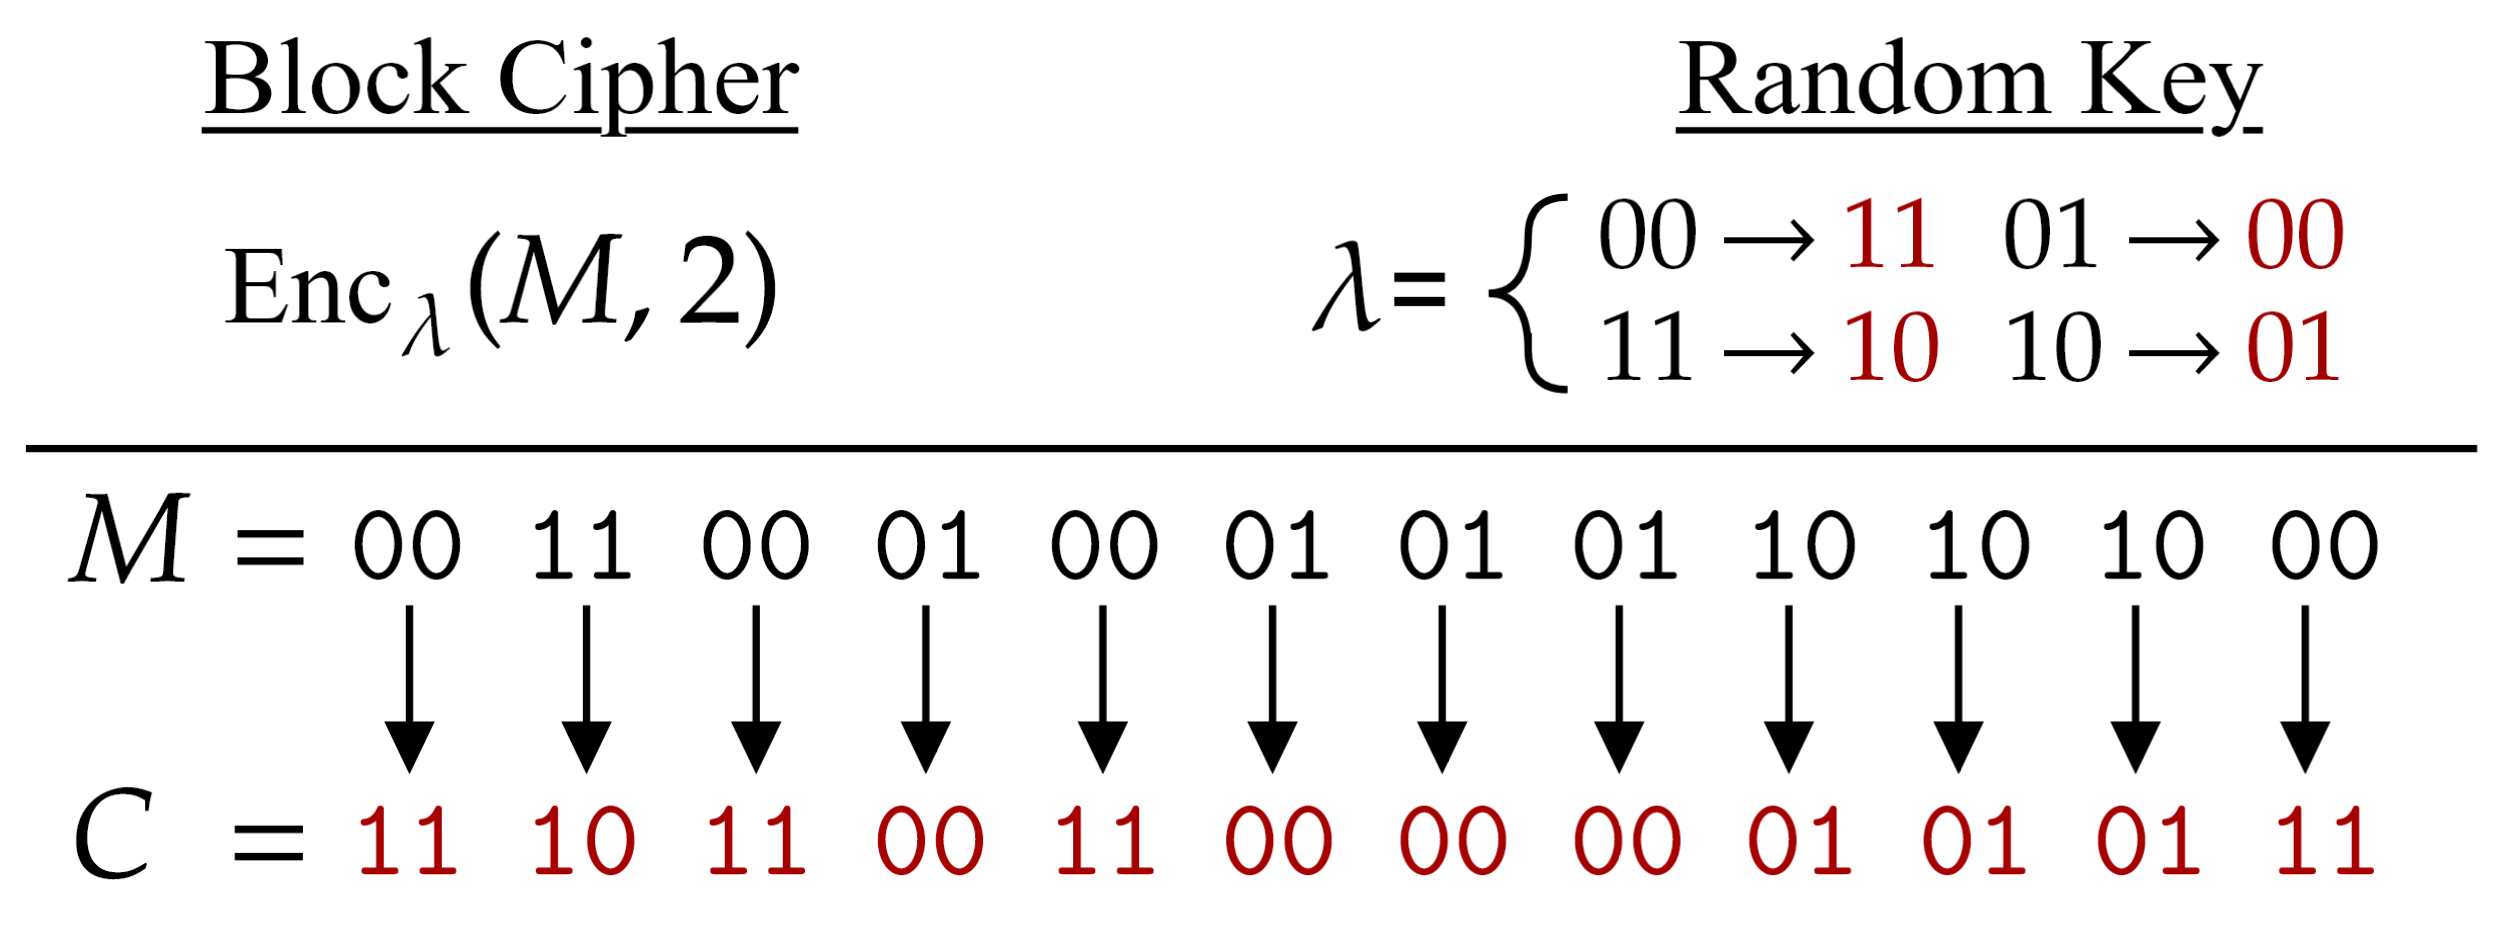
\includegraphics[width=.8\textwidth]{Sections/sec/enc/block.png}
    \caption{Electronic Codebook Mode (ECB) with a block size of 2 \cite{essex2024encrypting}.}
    \label{fig:block_cipher}
\end{figure}

\noindent
Though in its simplicity falls to the same weakness as the Caesar Cipher, as identical plaintext blocks will encrypt to the same ciphertext block.

\begin{figure}[h!]
    \centering
    \rule{\textwidth}{0.4pt}

    \vspace{1em}
    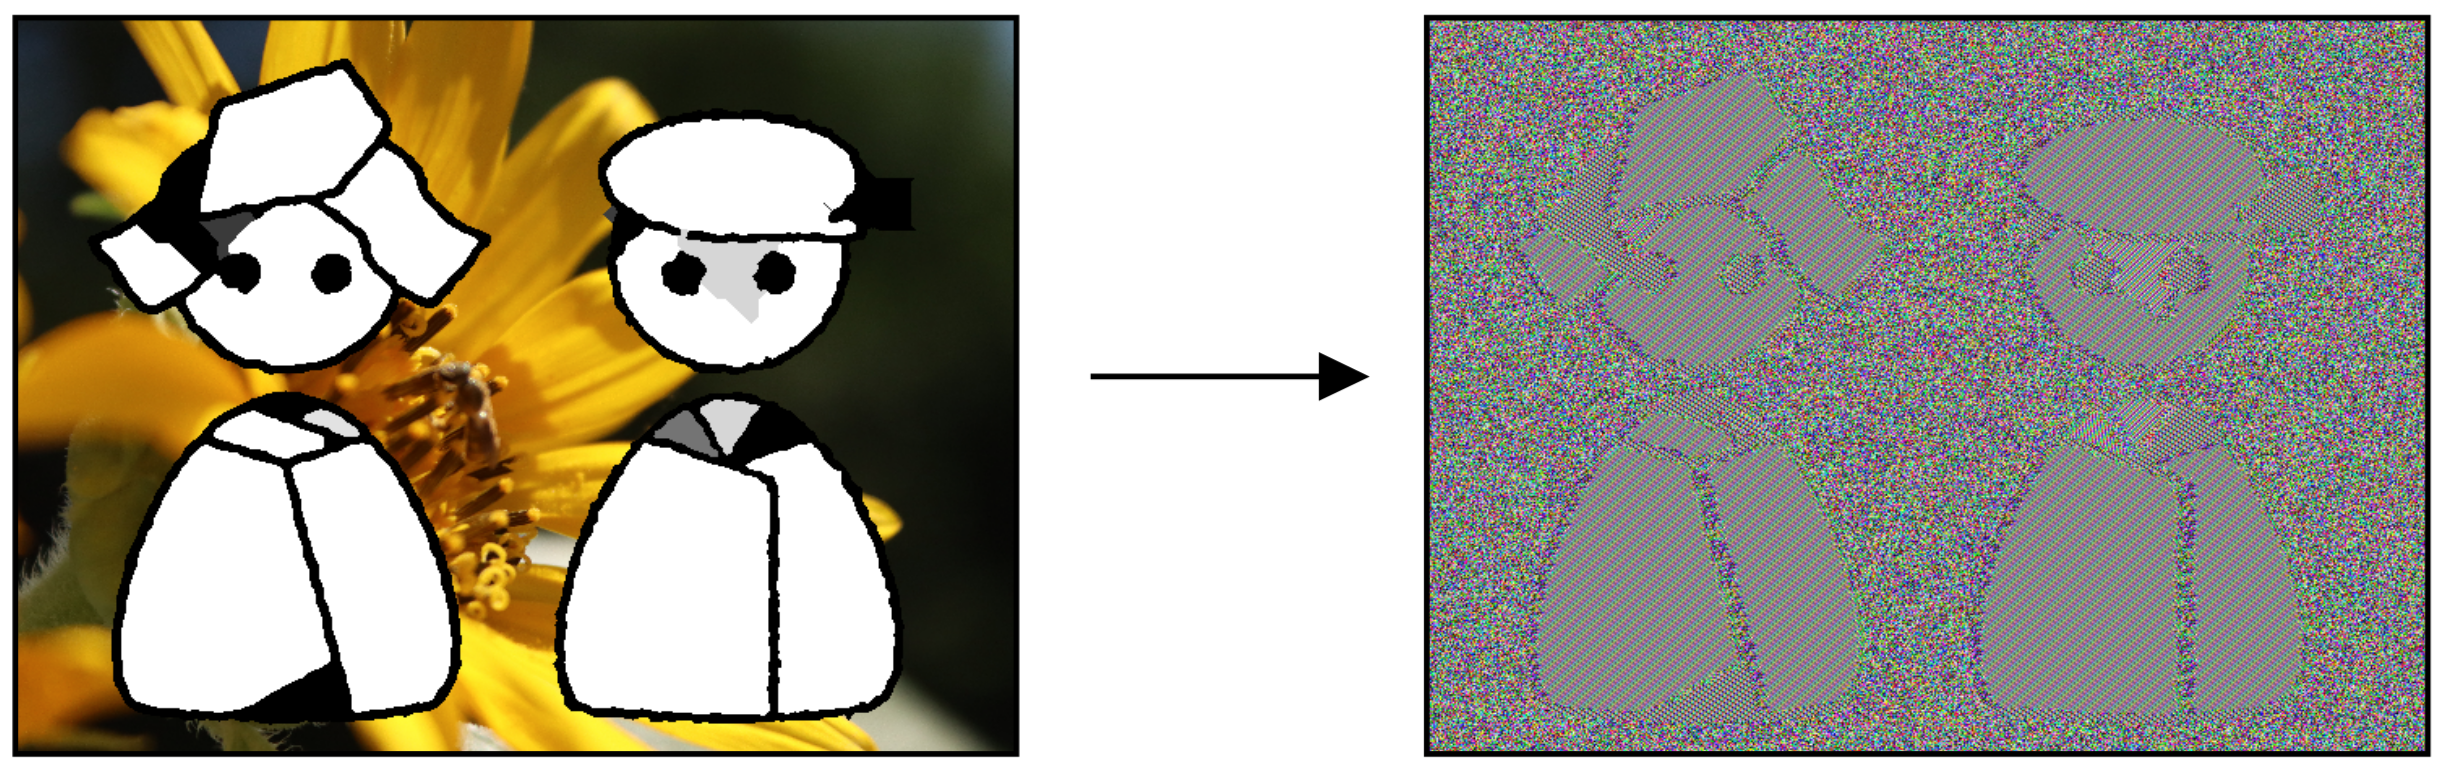
\includegraphics[width=.8\textwidth]{Sections/sec/enc/ecb.png}
    \rule{\textwidth}{0.4pt}
    \caption{An unencrypted image (left) and the same image encrypted with ECB (right).}
    \label{fig:block_cipher}
\end{figure}

\noindent
Here the image on the right is still partially recognizable, as when ECB encountered white space, it encrypted it to the same block.
Shockingly the popular video conferencing software Zoom used ECB during the 2020 COVID-19 pandemic, of which now has been patched.

\vspace{1em}
\begin{Def}[Cipher Block Chaining (CBC)]

    \label{theo:cipher_block_chaining}
    CBC encrypts blocks of plaintext into ciphertext. CBC uses a \textbf{Initialization Vector (IV)} to start the chain of XORing.
    The IV is XORed with the first plaintext block. Each XOR is indexed into the key value pair dictionary $\lambda$. The result is the cypher text block.
    Then the ciphertext block XORs with the next plaintext block and so on. \hfill \cite{nist80038a}\\
    \noindent
    \rule{\textwidth}{0.4pt}
    \textbf{Security Definition}: Confidentiality. Integrity and Authenticity are not guaranteed.
\end{Def}

\newpage 

\noindent
The below figure demonstrates use of a block cipher with the Cipher Block Chaining Mode (CBC).

\begin{figure}[h!]
    \centering
    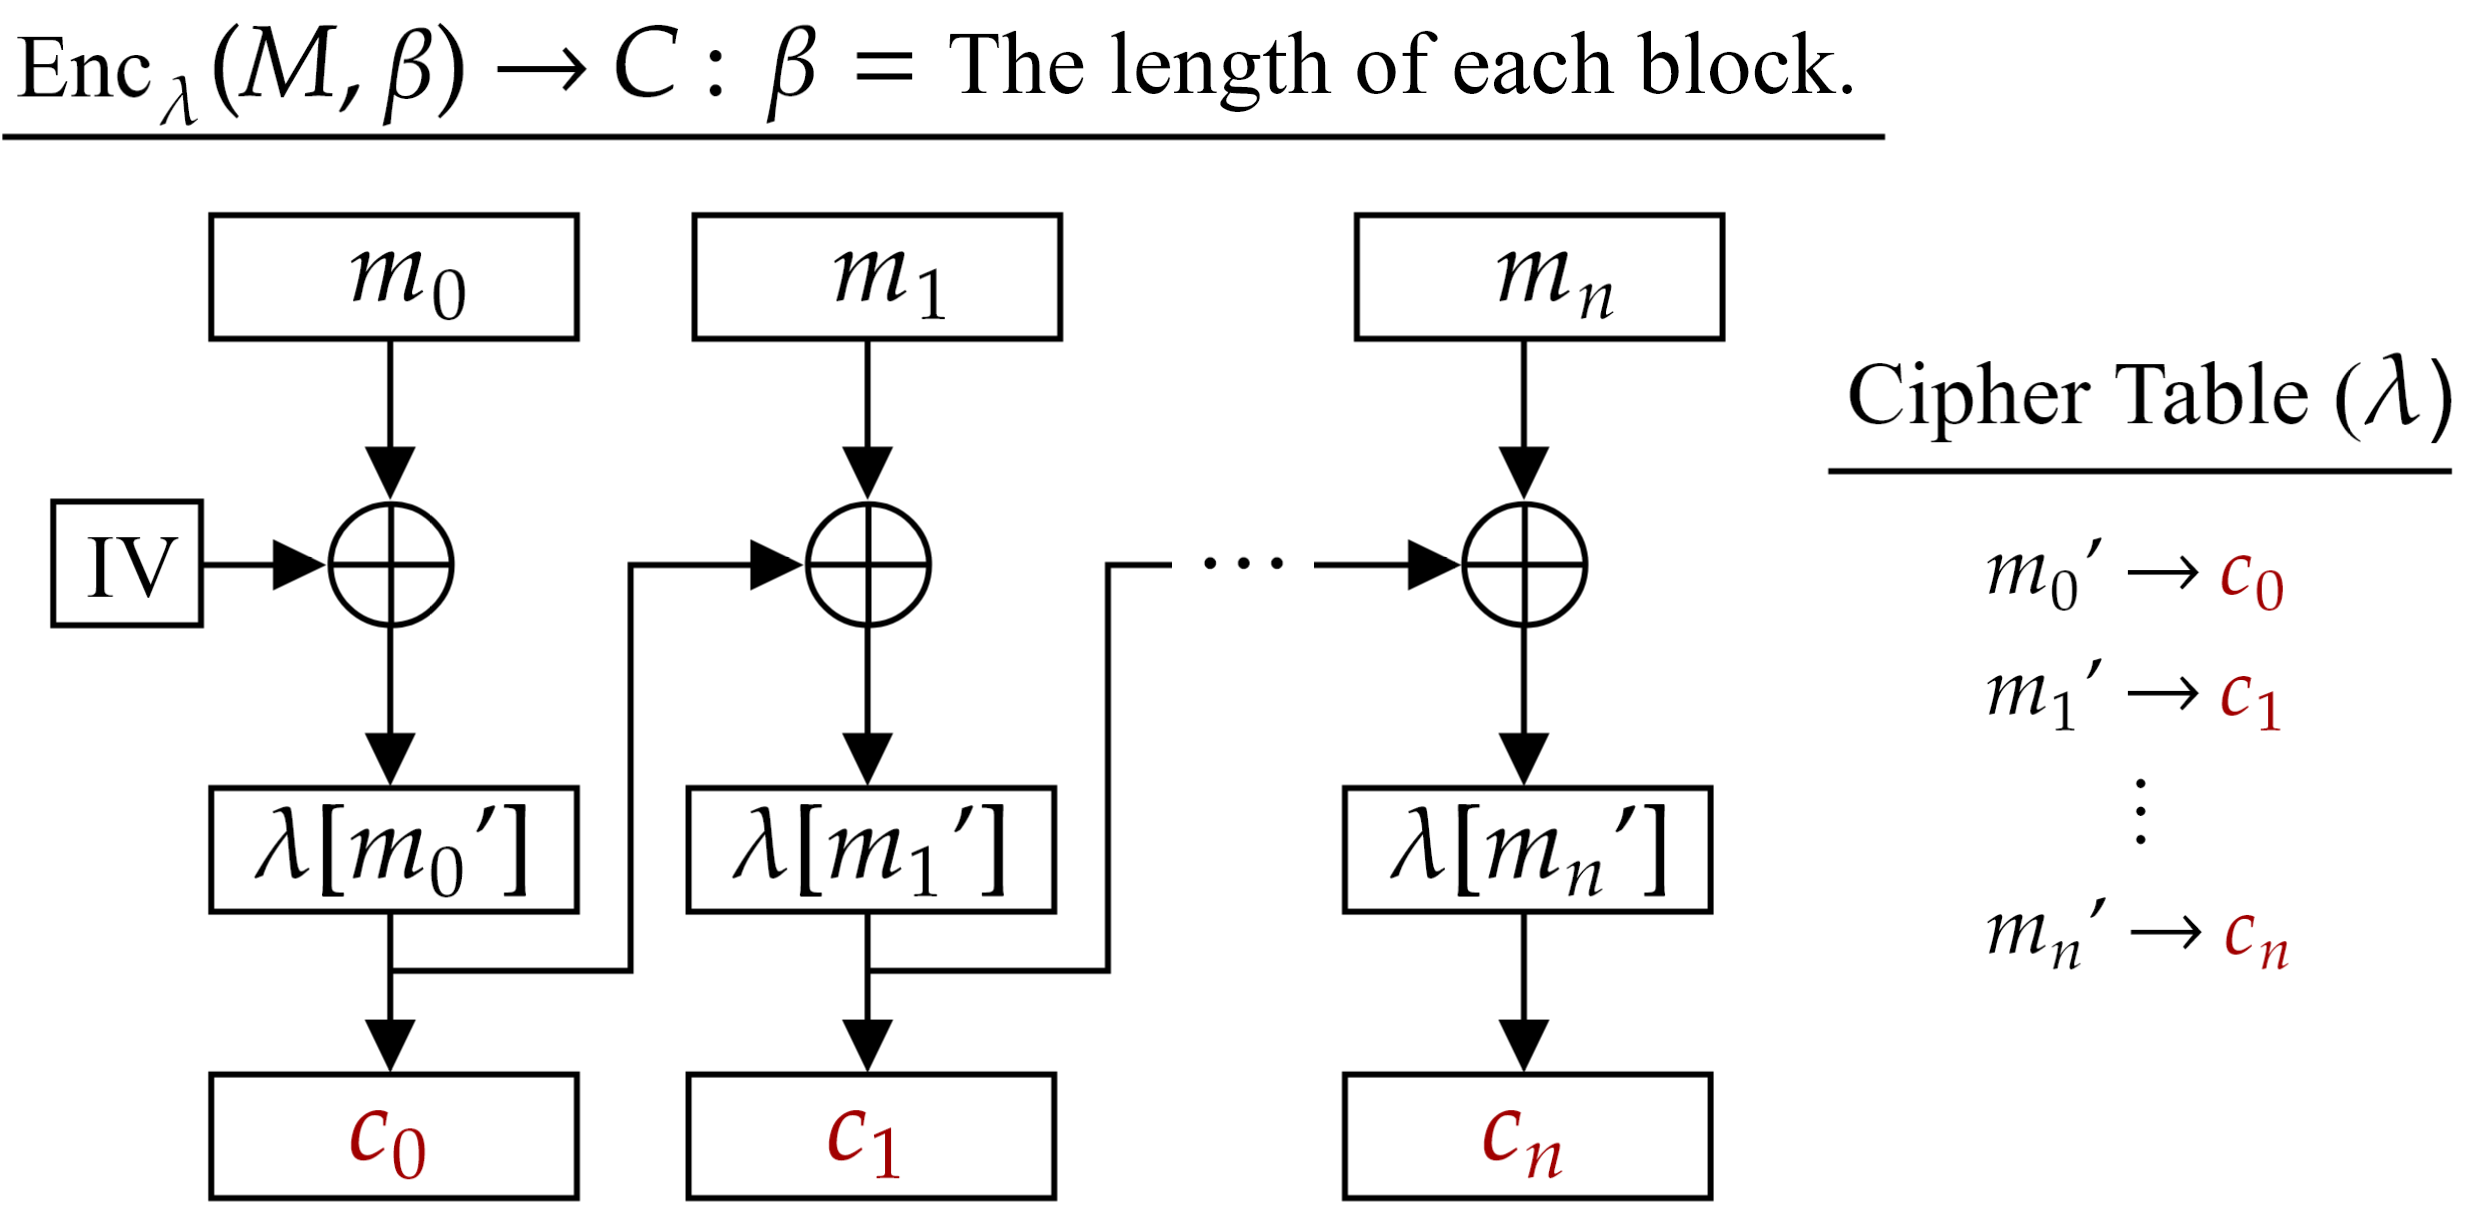
\includegraphics[width=.8\textwidth]{Sections/sec/enc/cbc.png}
    \caption{A block cipher utilizing the Cipher Block Chaining Mode (CBC) method. \cite{essex2024encrypting}.}
    \label{fig:block_cipher}
\end{figure}

\vspace{-1em}
\begin{figure}[h!]
    \centering
    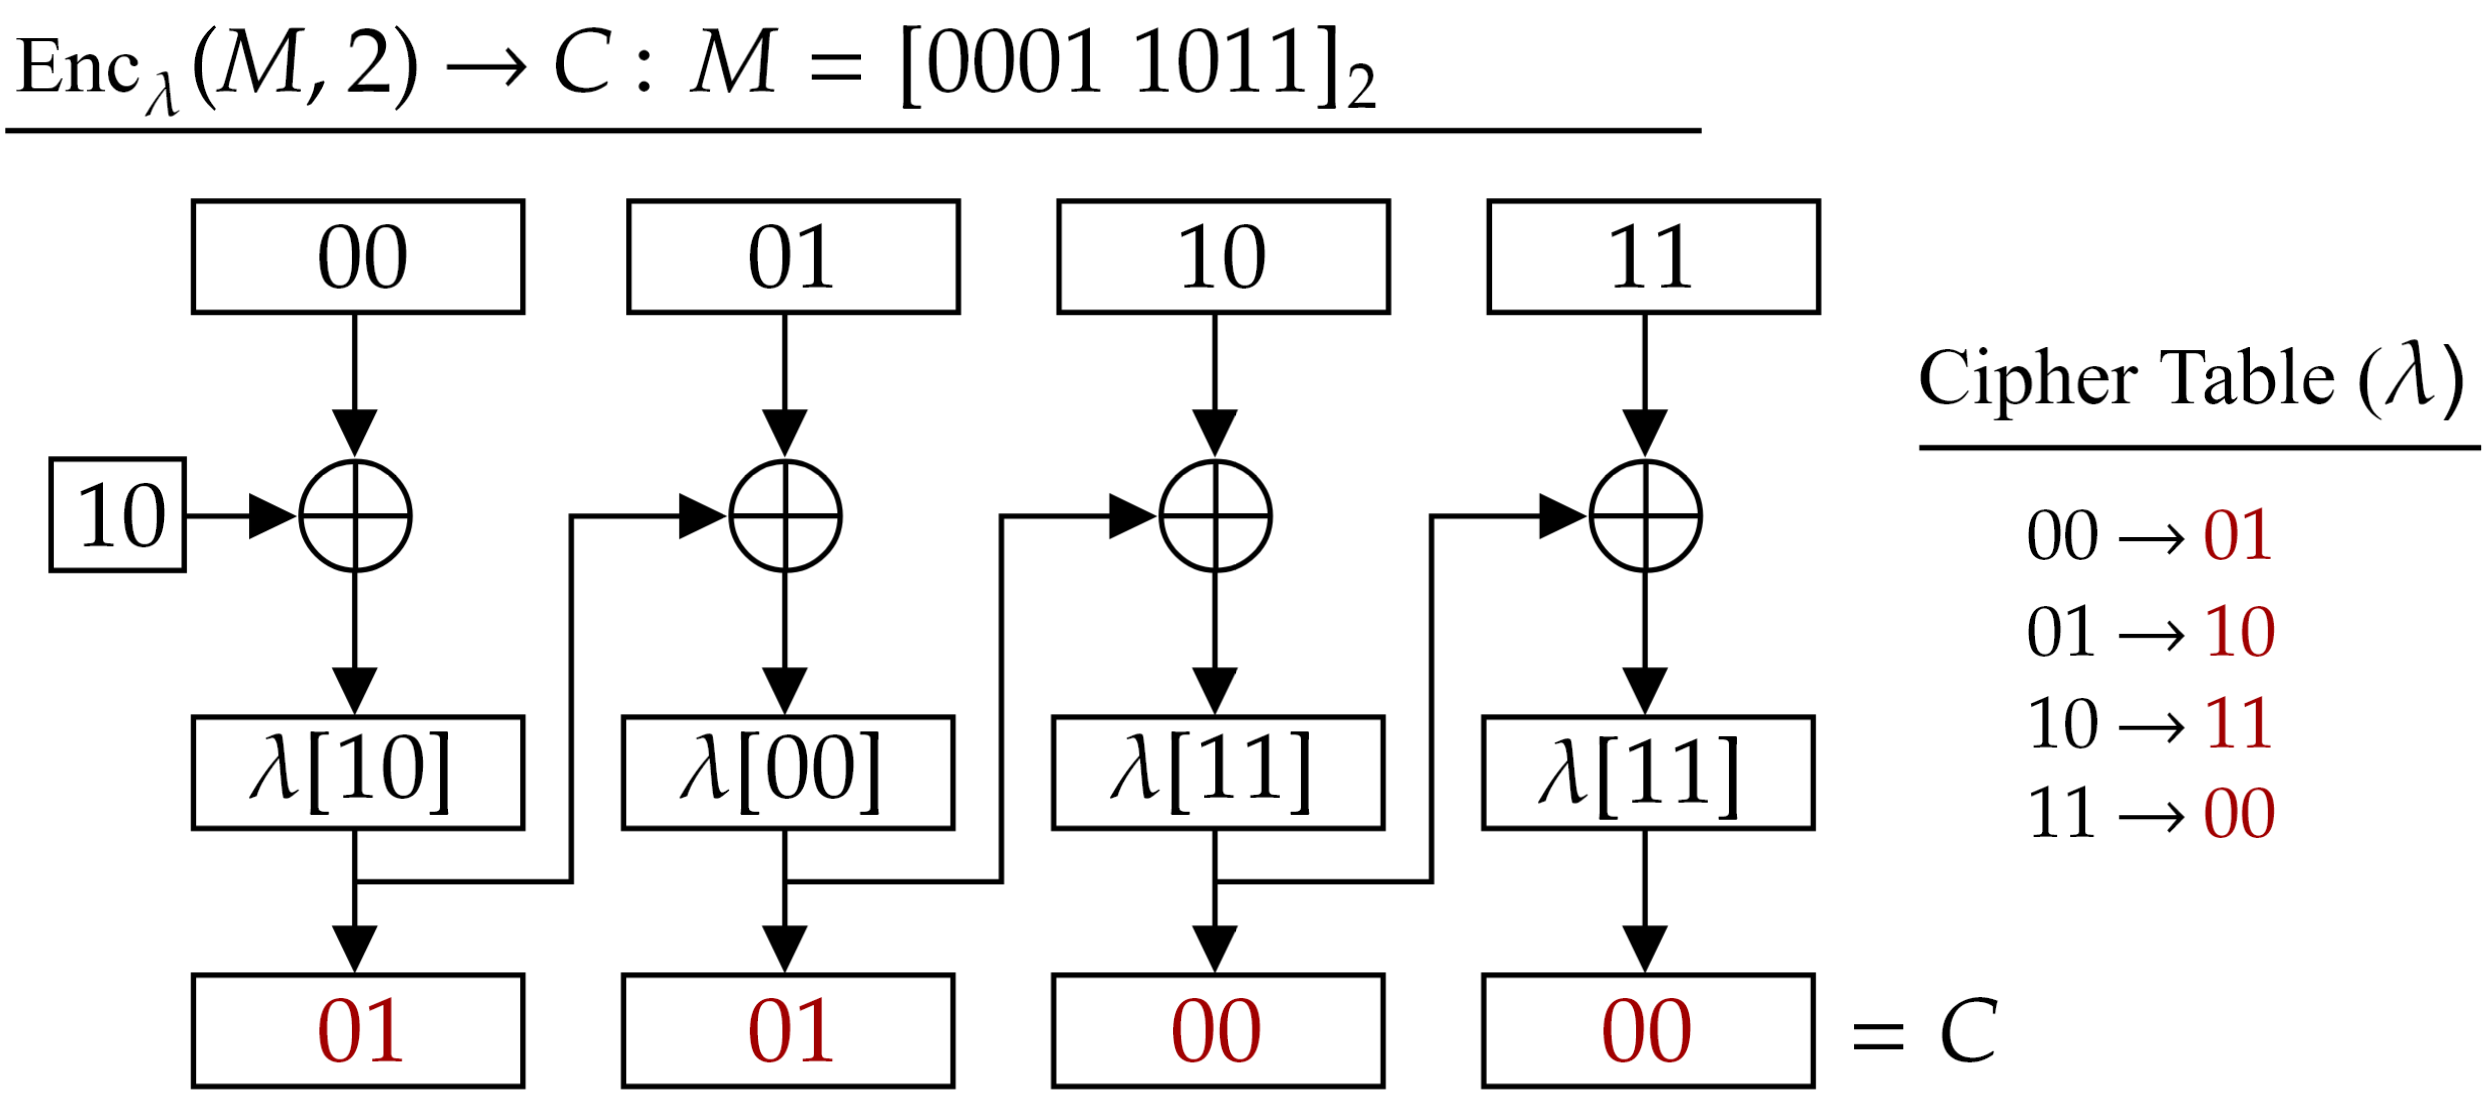
\includegraphics[width=.8\textwidth]{Sections/sec/enc/cbc_ex.png}
    \caption{CBC encryption example with input $[0001\ 1011]_2$ and outputs $[0101\ 0000]_2$.}
    \label{fig:block_cipher}
\end{figure}

\noindent
Plenty of block cyphers elaborate on these concepts. The different flavors are called a \textbf{mode of operation}.

\begin{Def}[Message Authentication Code (MAC)]

    \label{theo:mac}
    A MAC combines a message with a secret key before hashing.
    Let $M$ be the message, $\lambda$ the key, and the function $T\gets$Enc$_\lambda(M)$. Where $T$ is a resulting tag, sometimes called 
    a \textbf{digest} or \textbf{hash}. Then $(M,T)$ is sent over the wire. The receiver also has $\lambda$ and runs Enc$_\lambda(M)$ to verify $T$.\\
    \noindent
    \rule{\textwidth}{0.4pt}
    \textbf{Security Definition}: Integrity and Authenticity. Not confidentiality.
\end{Def}

\newpage 
\noindent
The following figure demonstrates that a MAC protects integrity, as if the message were altered, the receiver would 
not get the same tag with their key. Though an adversary may still intercept and read the message.

\begin{figure}[h!]
    \centering
    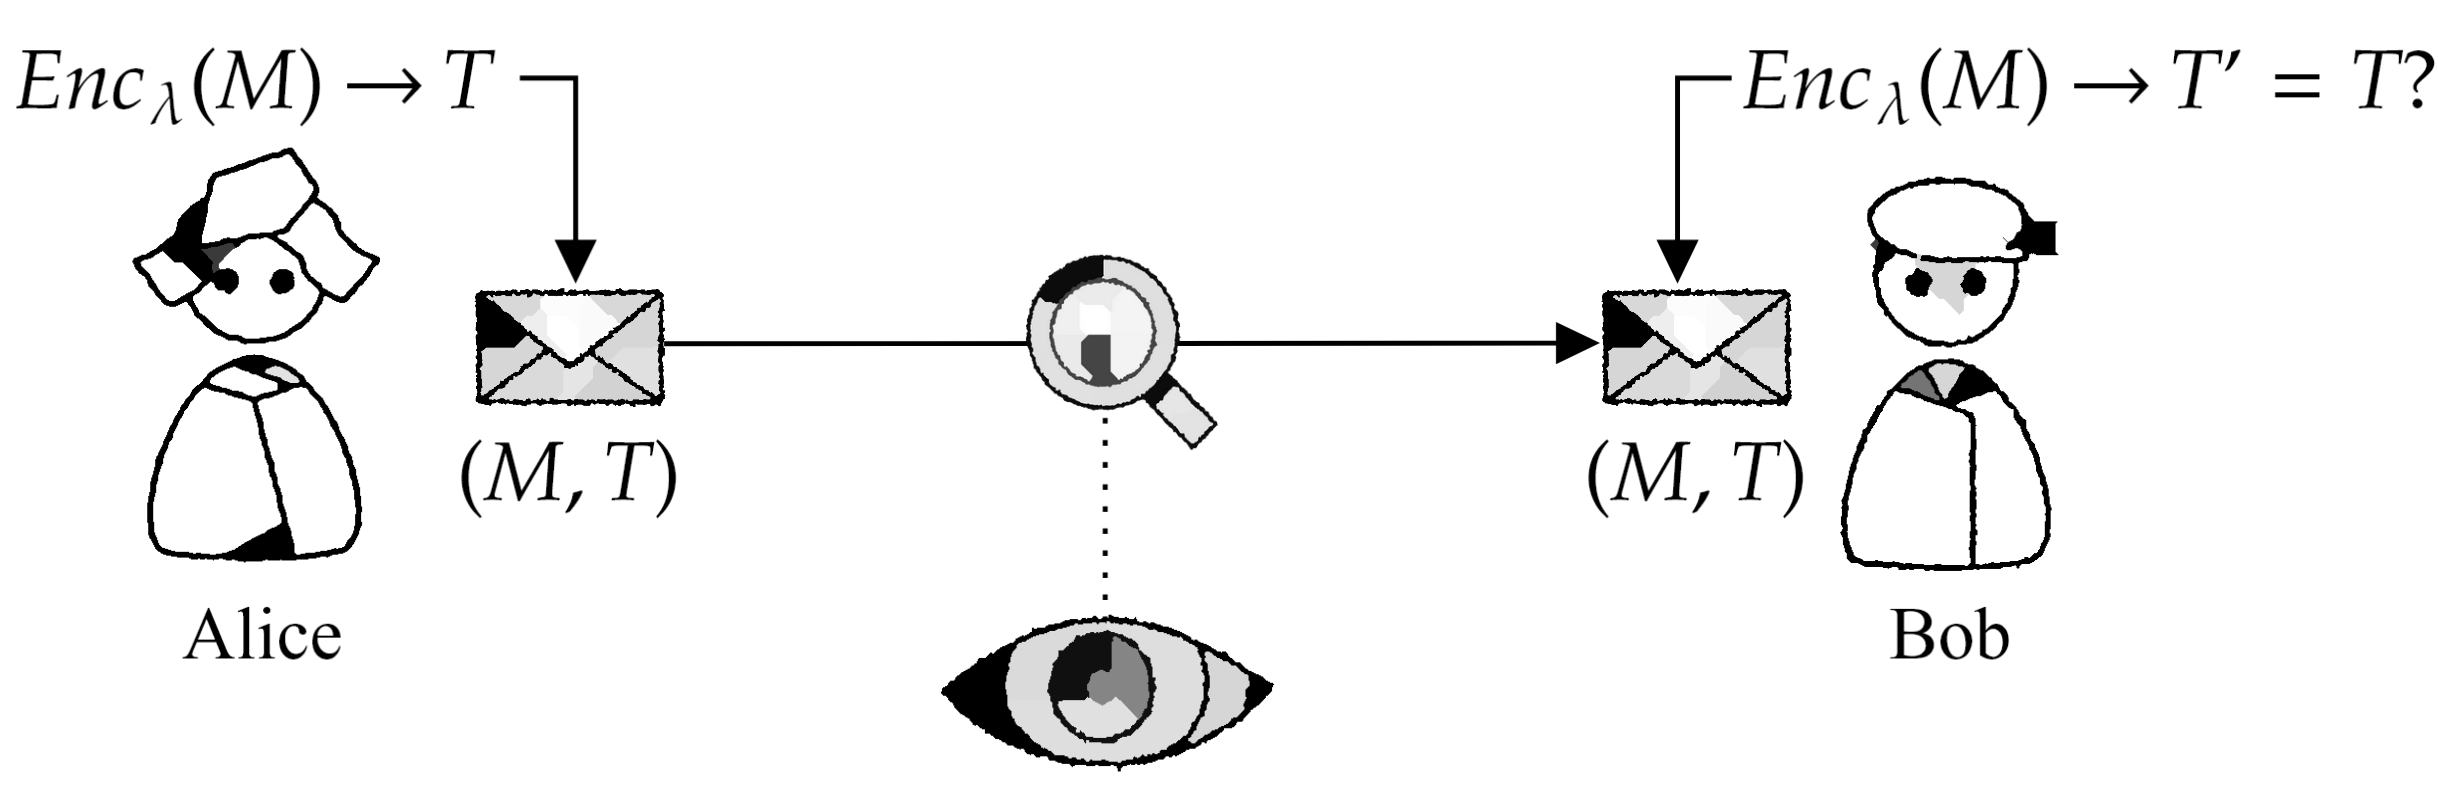
\includegraphics[width=.8\textwidth]{Sections/sec/enc/mac.png}
    \caption{A MAC protecting integrity.}
    \label{fig:block_cipher}
\end{figure}

\begin{theo}[Replay Attack]

    \label{theo:replay_attack}
    A replay attack is when an adversary intercepts a message and resends it to the receiver. The receiver may not know the message was sent twice.
\end{theo}

\begin{figure}[h!]
    \centering
    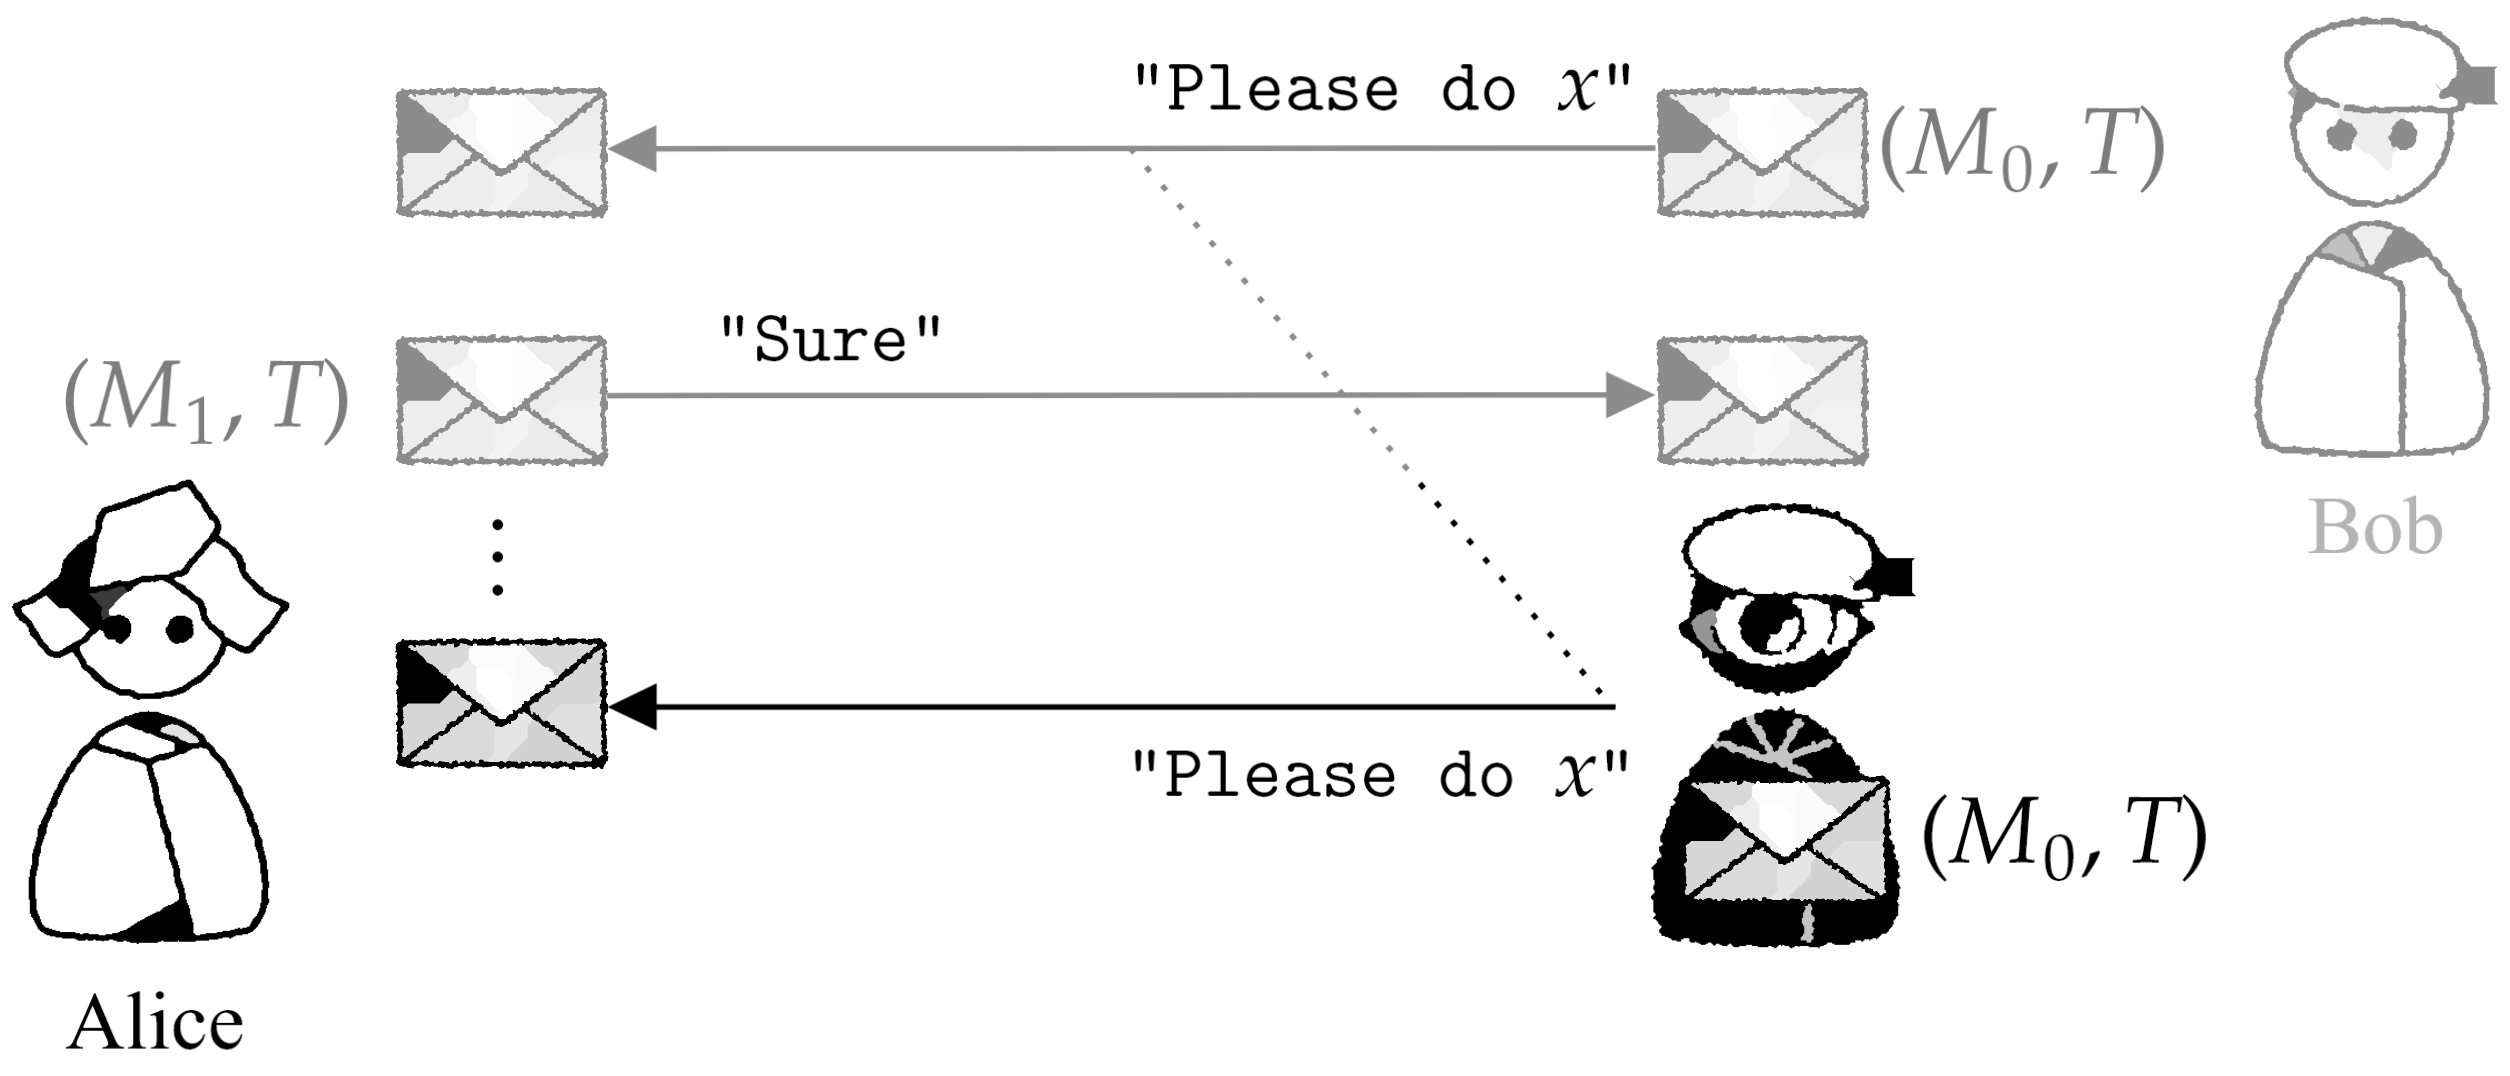
\includegraphics[width=.8\textwidth]{Sections/sec/enc/replay.png}
    \caption{A replay attack, where the adversary intercepts and resends a message.}
    \label{fig:block_cipher}
\end{figure}

\begin{theo}[Replay Attack Prevention]

    \label{theo:replay_attack_prevention}
    To prevent replay attacks, a timestamp or nonce (number used once) is added to the message. The receiver checks the timestamp or nonce to ensure the message is fresh.
\end{theo}

\newpage 

\begin{Def}[Hashed-based Message Authentication Code (HMAC)]

    \label{theo:hmac}
    HMACs are a type of MAC which are standardized and deemed secure. They take a pre-defined 
    hash function (e.g., SHA-256) and apply it to a MAC. I.e., an HMAC is a specific recipe for a MAC. \hfill \cite{seth2013macvsHMAC}
\end{Def}

\section{Block Ciphers \& Modes of Operation}
\begin{Def}[Galios Counter Mode (GCM)]

    \label{theo:gcm}
    GCM uses a MAC called GMAC, which is a variant of the HMAC. It encrypts data 
    with a desired Encryption Algorithm and then GMACs (MACs) the data into cipher text. The final hash is the tag. This 
    process goes as follows:
    \begin{itemize}
        \item \textbf{Encryption}:
        \begin{enumerate}
            \item Each block of plaintext is XORed with the encryption key.
            \item To ensure randomness, a counter is added to each encryption before XORing.
            \item To ensure randomness of the counter, an IV is added to it.
        \end{enumerate}
        \item \textbf{MAC}:
        \begin{enumerate}
            \item After encryption, the data is XORed with a previous hash then GMACed.
            \item The GMAC is then used to XOR the next block's cipher before hashing again.
            \item To start the chain of XORing, a 128-bits of zeros is encrypted and GMACed.
            \item After the final block, the length of the message is XORed with the prior hash, then GMACed.
            \item Finally, an encryption of 32-bits of zeros is XORed with the final hash, producing the tag.
        \end{enumerate}
    \end{itemize}

    \noindent
    GCM also supports \textbf{Authentication of Additional Data (AAD)}, which is data that is not encrypted but is still hashed.
    So in addition to authenticating and encrypting a message, GCM can also authenticate additional unencrypted data.
    If GCM is only used for authentication, it is called \textbf{GMAC}. \hfill \cite{vidder_gcm_gmac}
    \noindent
    \rule{\textwidth}{0.4pt}
    \textbf{Security Definition}: Confidentiality, Integrity, and Authenticity.
\end{Def}

\vfill
\begin{center}
    \textit{GCM Diagram and Elaborations on the next page.}
\end{center}
\vfill 

\newpage

\noindent
The following figures are first broken up and then combined for clarity.\\

\begin{figure}[h!]
    \centering
    \hfill{1em}
    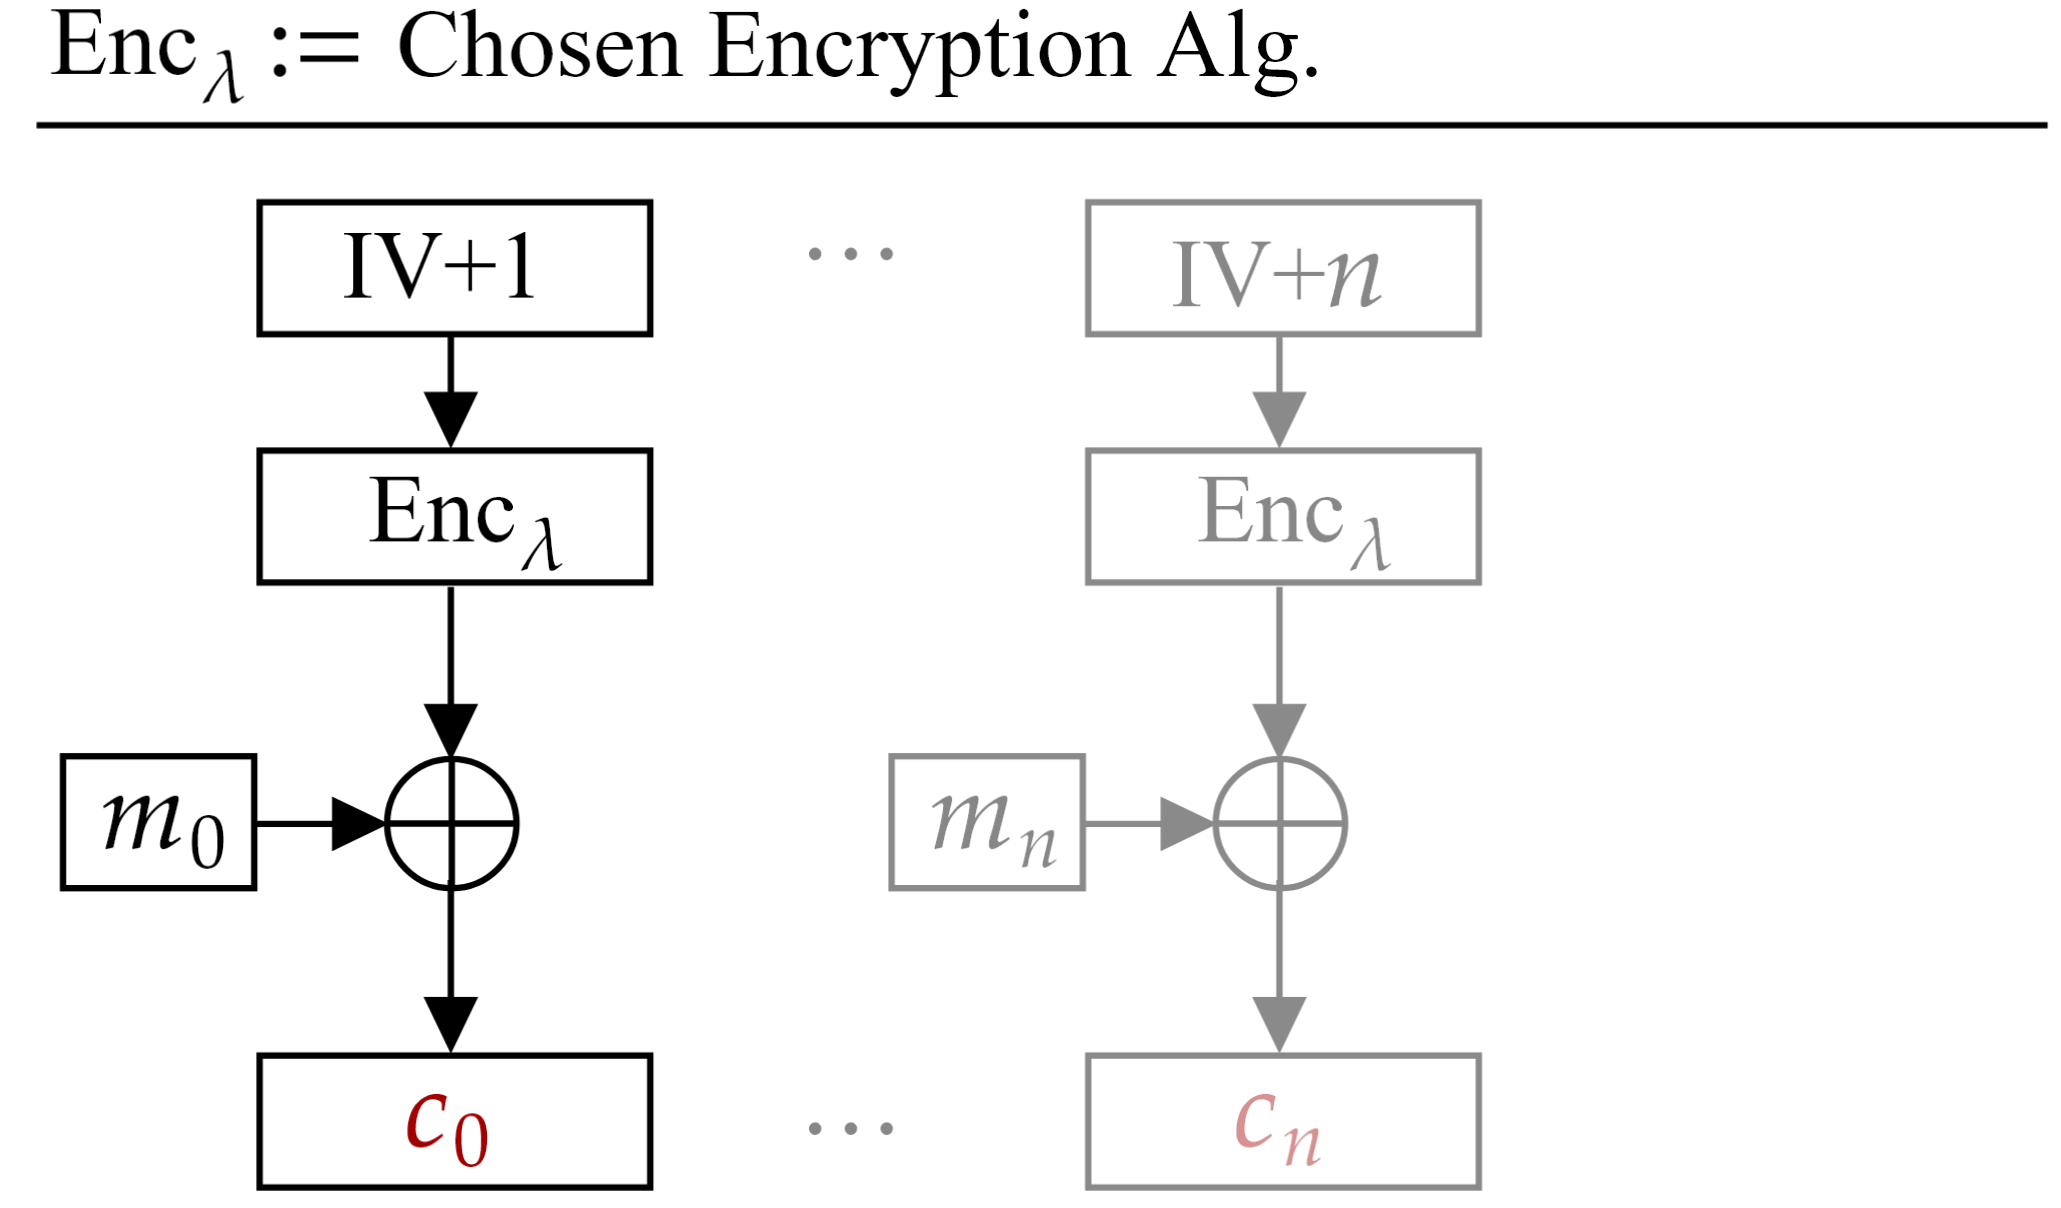
\includegraphics[width=.8\textwidth]{Sections/sec/enc/iv.png}
    \caption{GCM IV and Counter XORing with Plaintext to create Ciphertext.}
    \label{fig:block_cipher}
\end{figure}

\begin{figure}[h!]
    \centering
    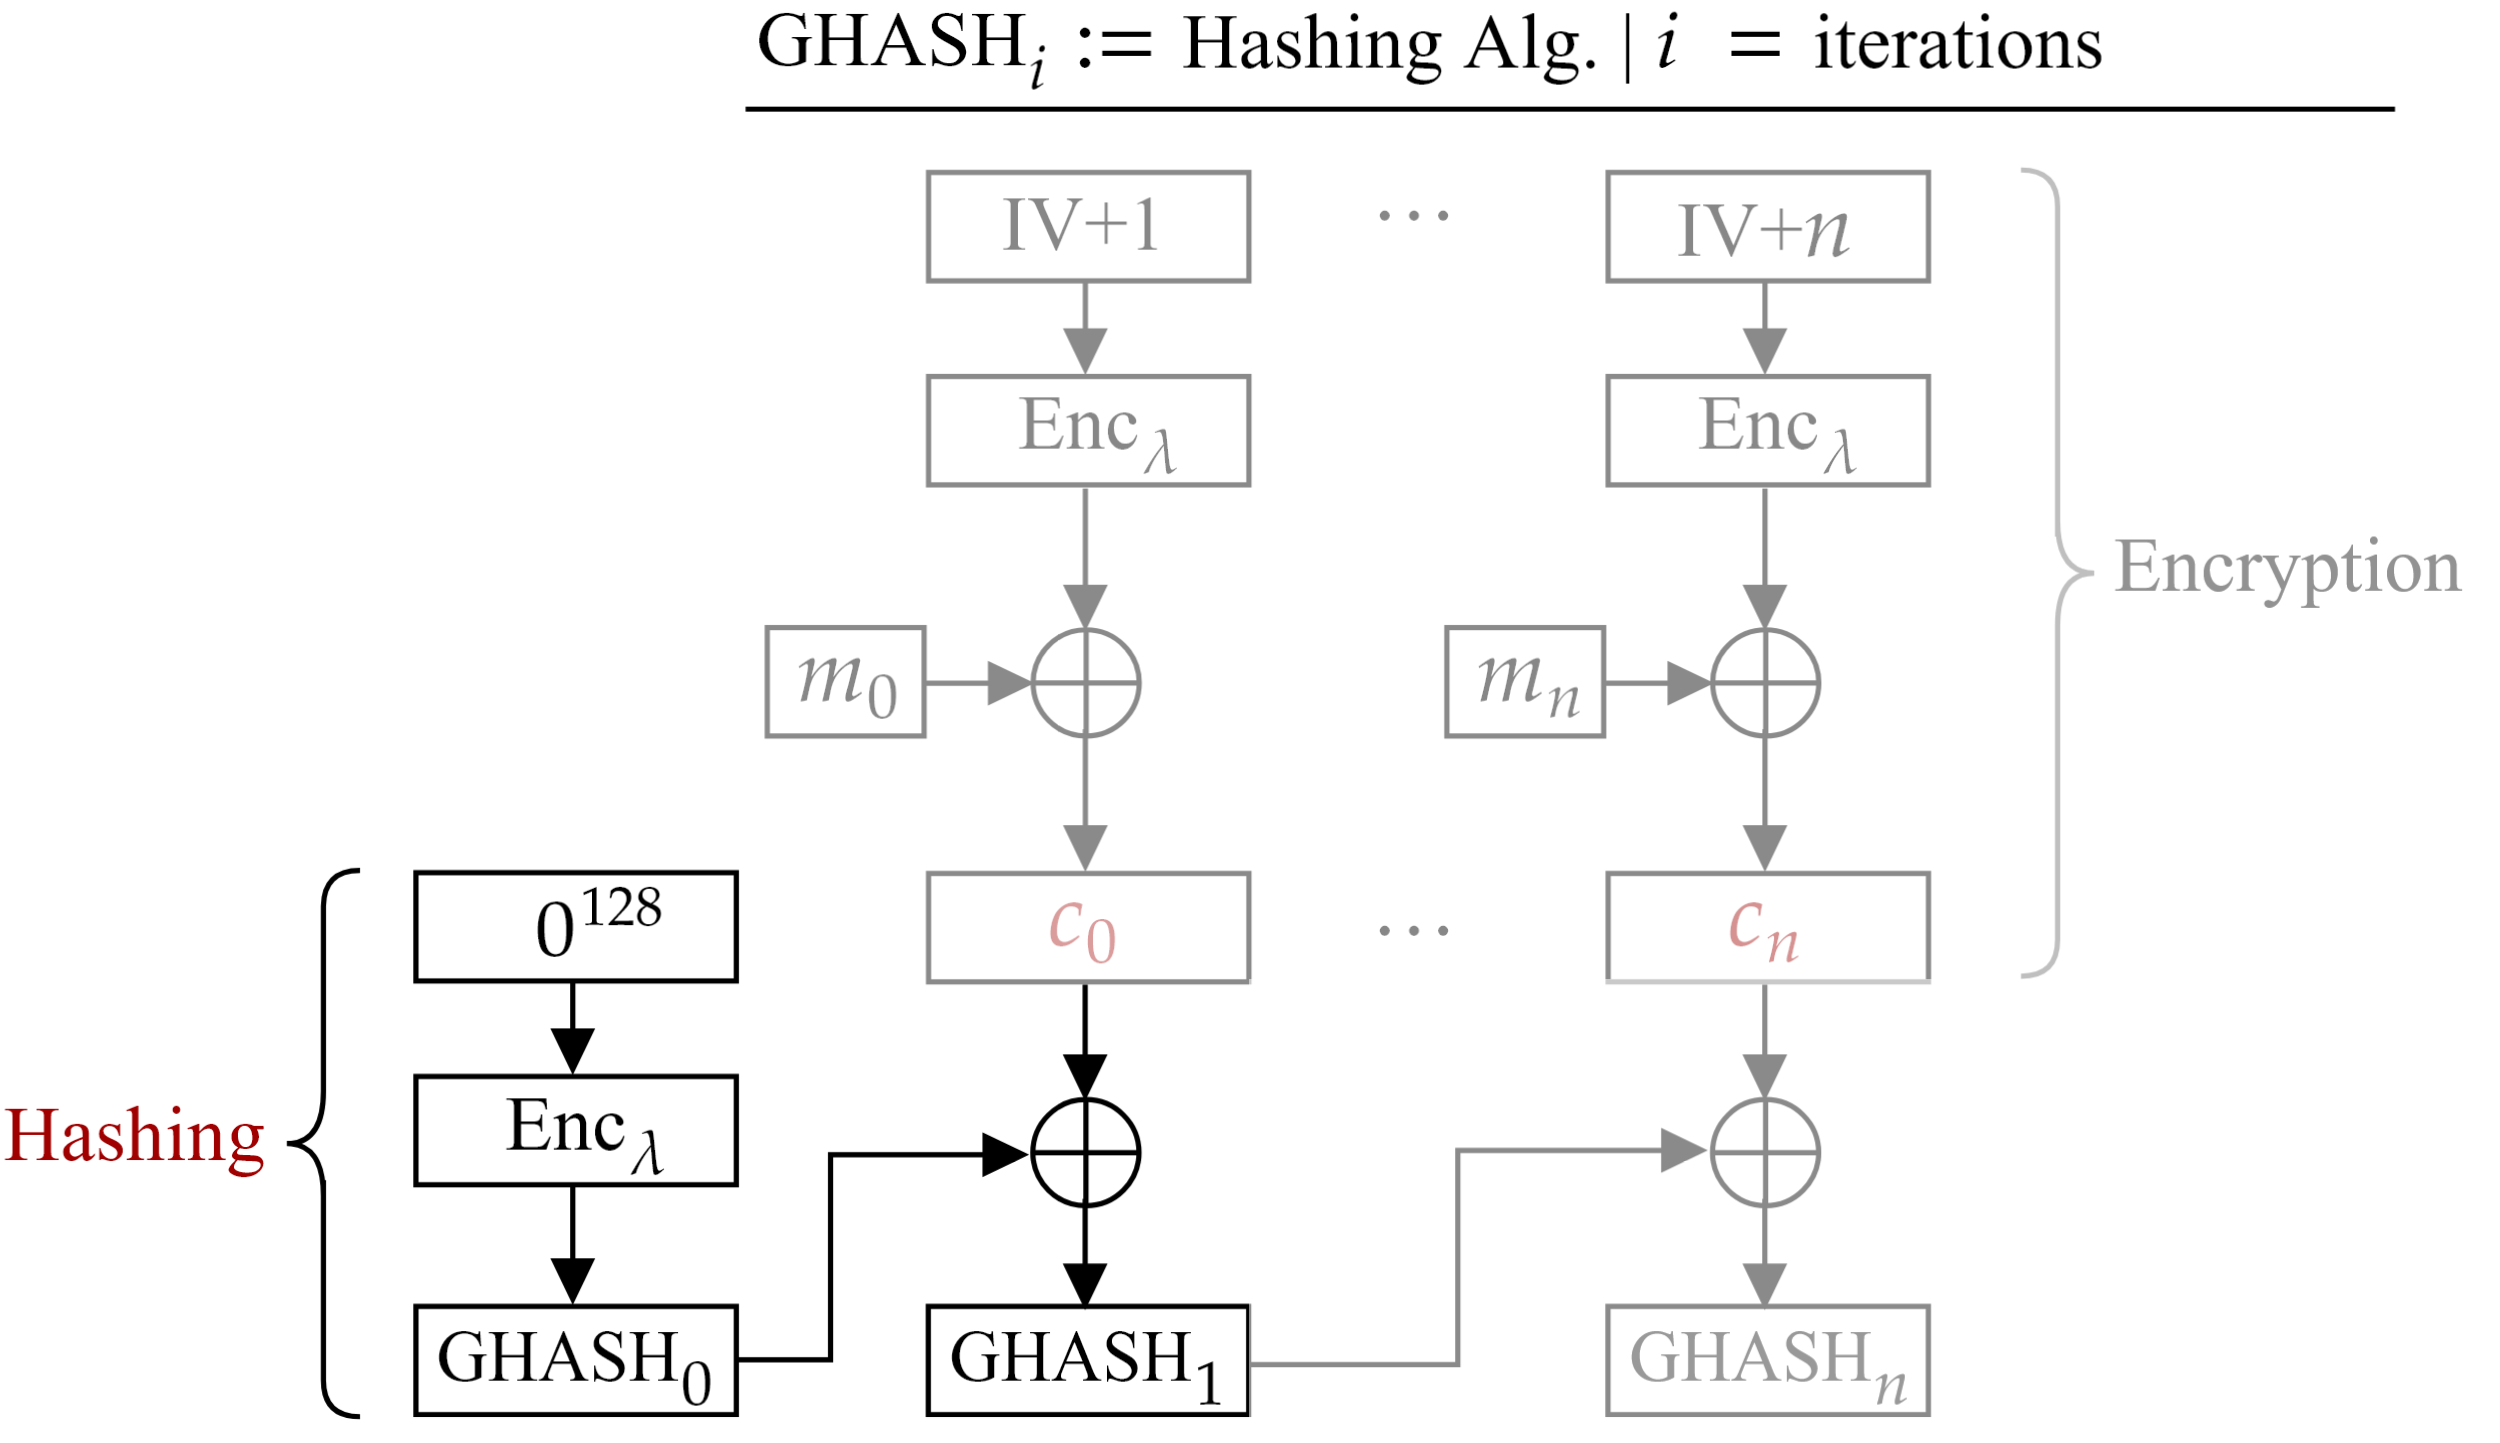
\includegraphics[width=.9\textwidth]{Sections/sec/enc/ghash.png}
    \caption{128-bits of zeros is encrypted and GMACed, starting the chain of XOR hashing.}
    \label{fig:block_cipher}
\end{figure}
\vfill
\begin{center}
    \textit{Continued on the next page.}
\end{center}
\vfill 
\newpage 

\noindent
To finish the chain of XOR hashing:
\begin{figure}[h!]
    \centering
    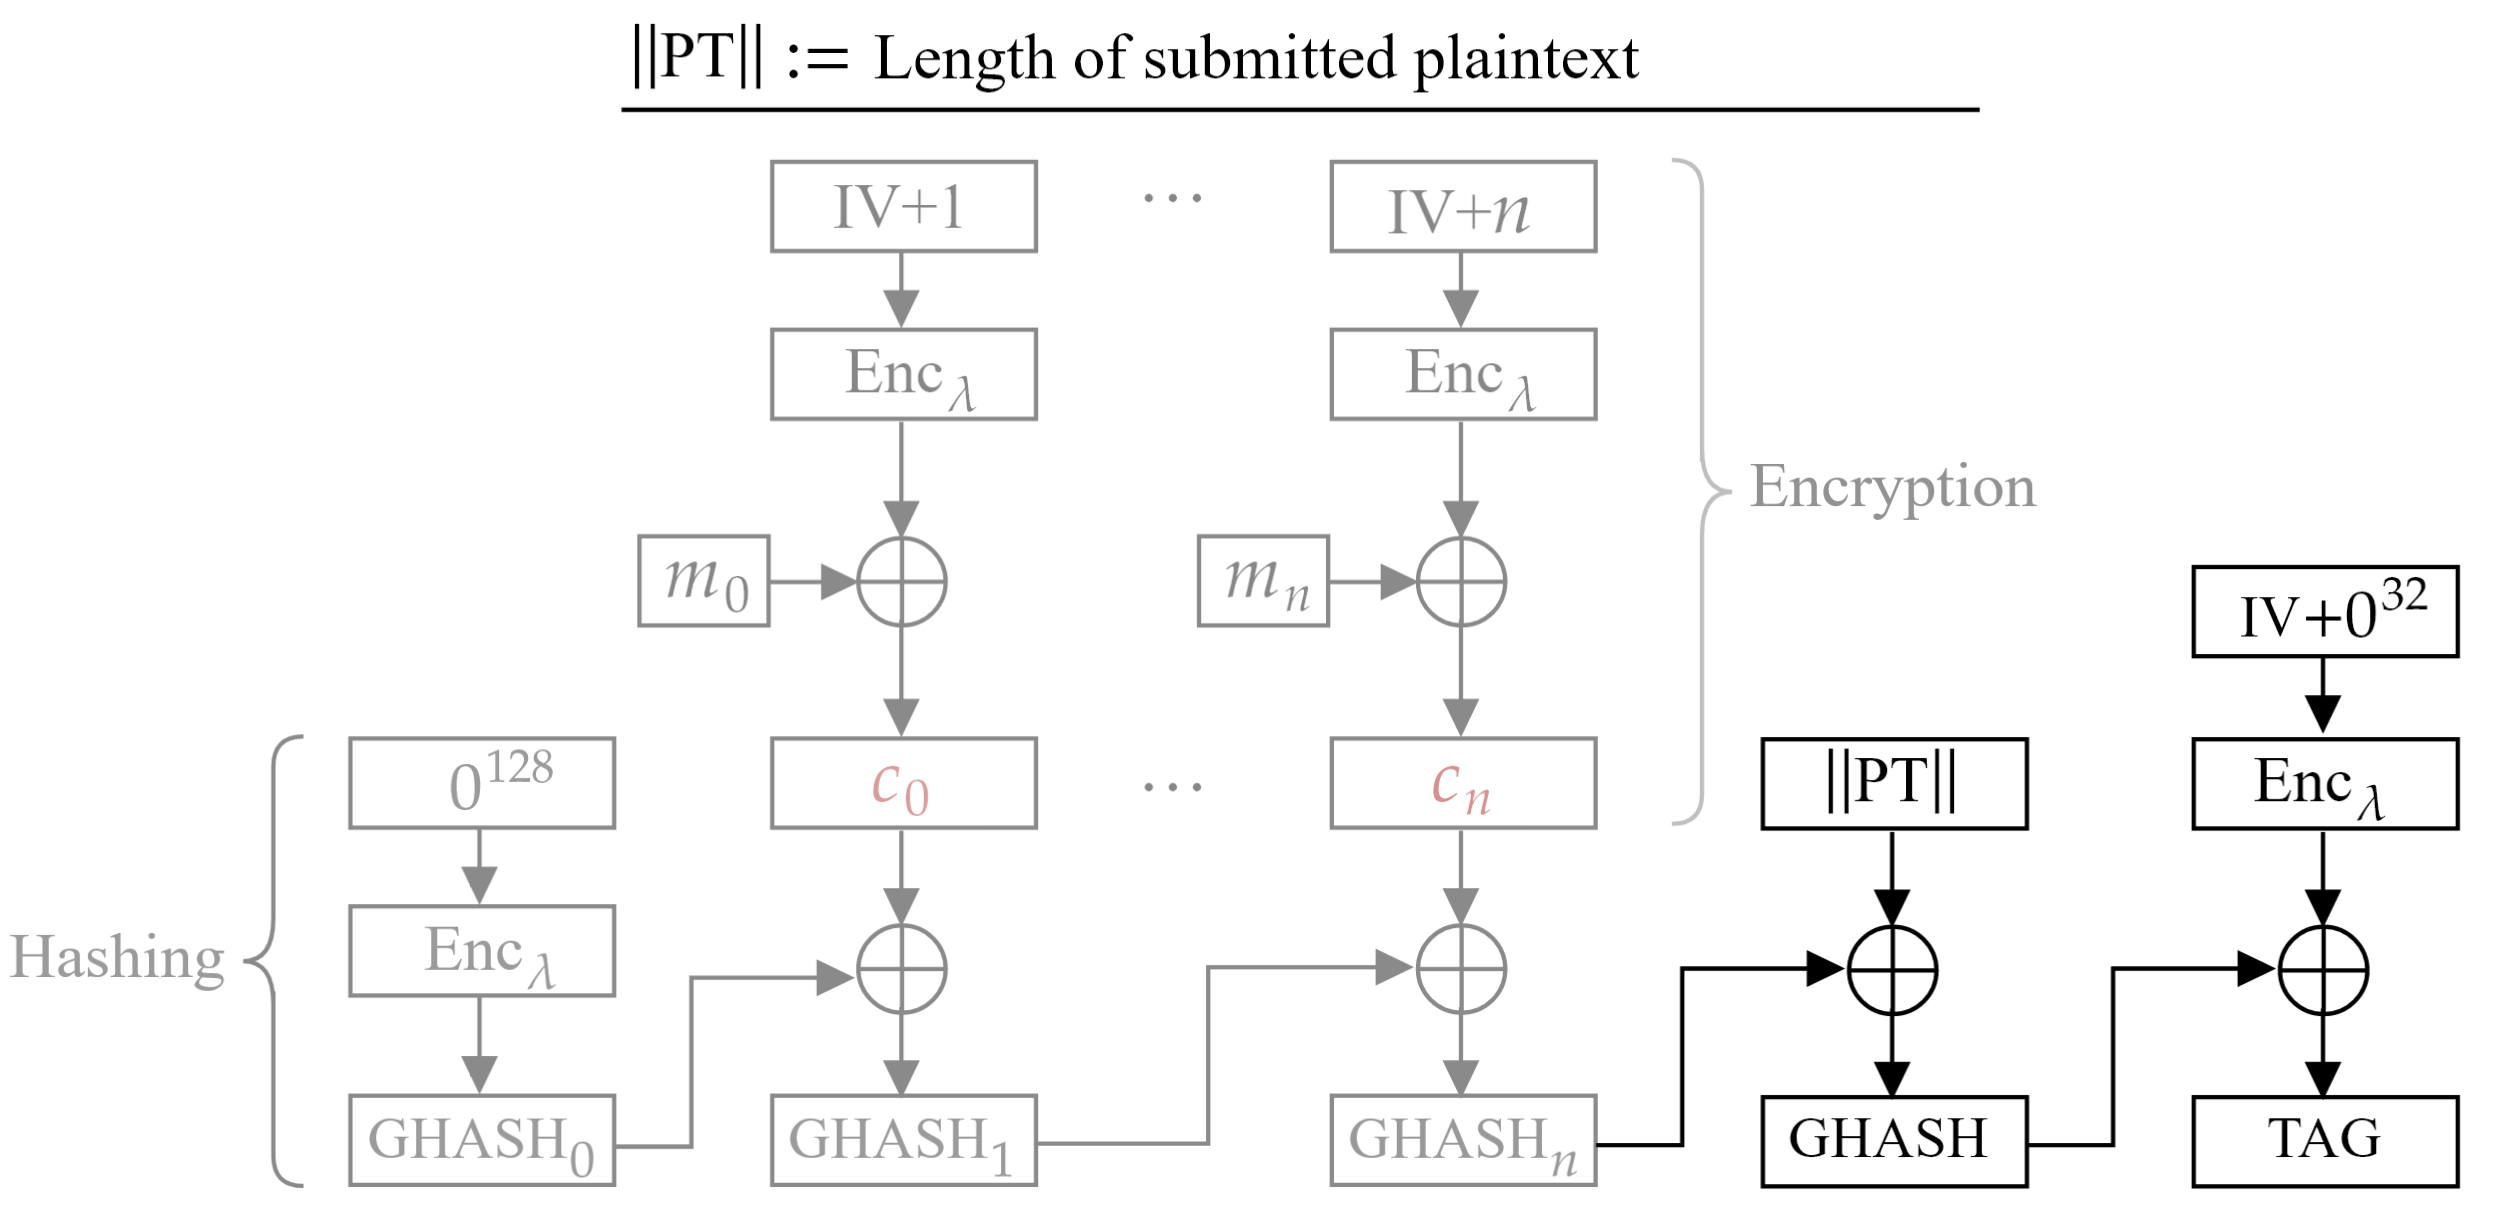
\includegraphics[width=1\textwidth]{Sections/sec/enc/len.png}
    \caption{The length of the message is XORed with the prior hash, then GMACed with 32-bits of encrypted zeros concatenated with the IV.}
    \label{fig:block_cipher}
\end{figure}

\begin{figure}[h!]
    \centering

    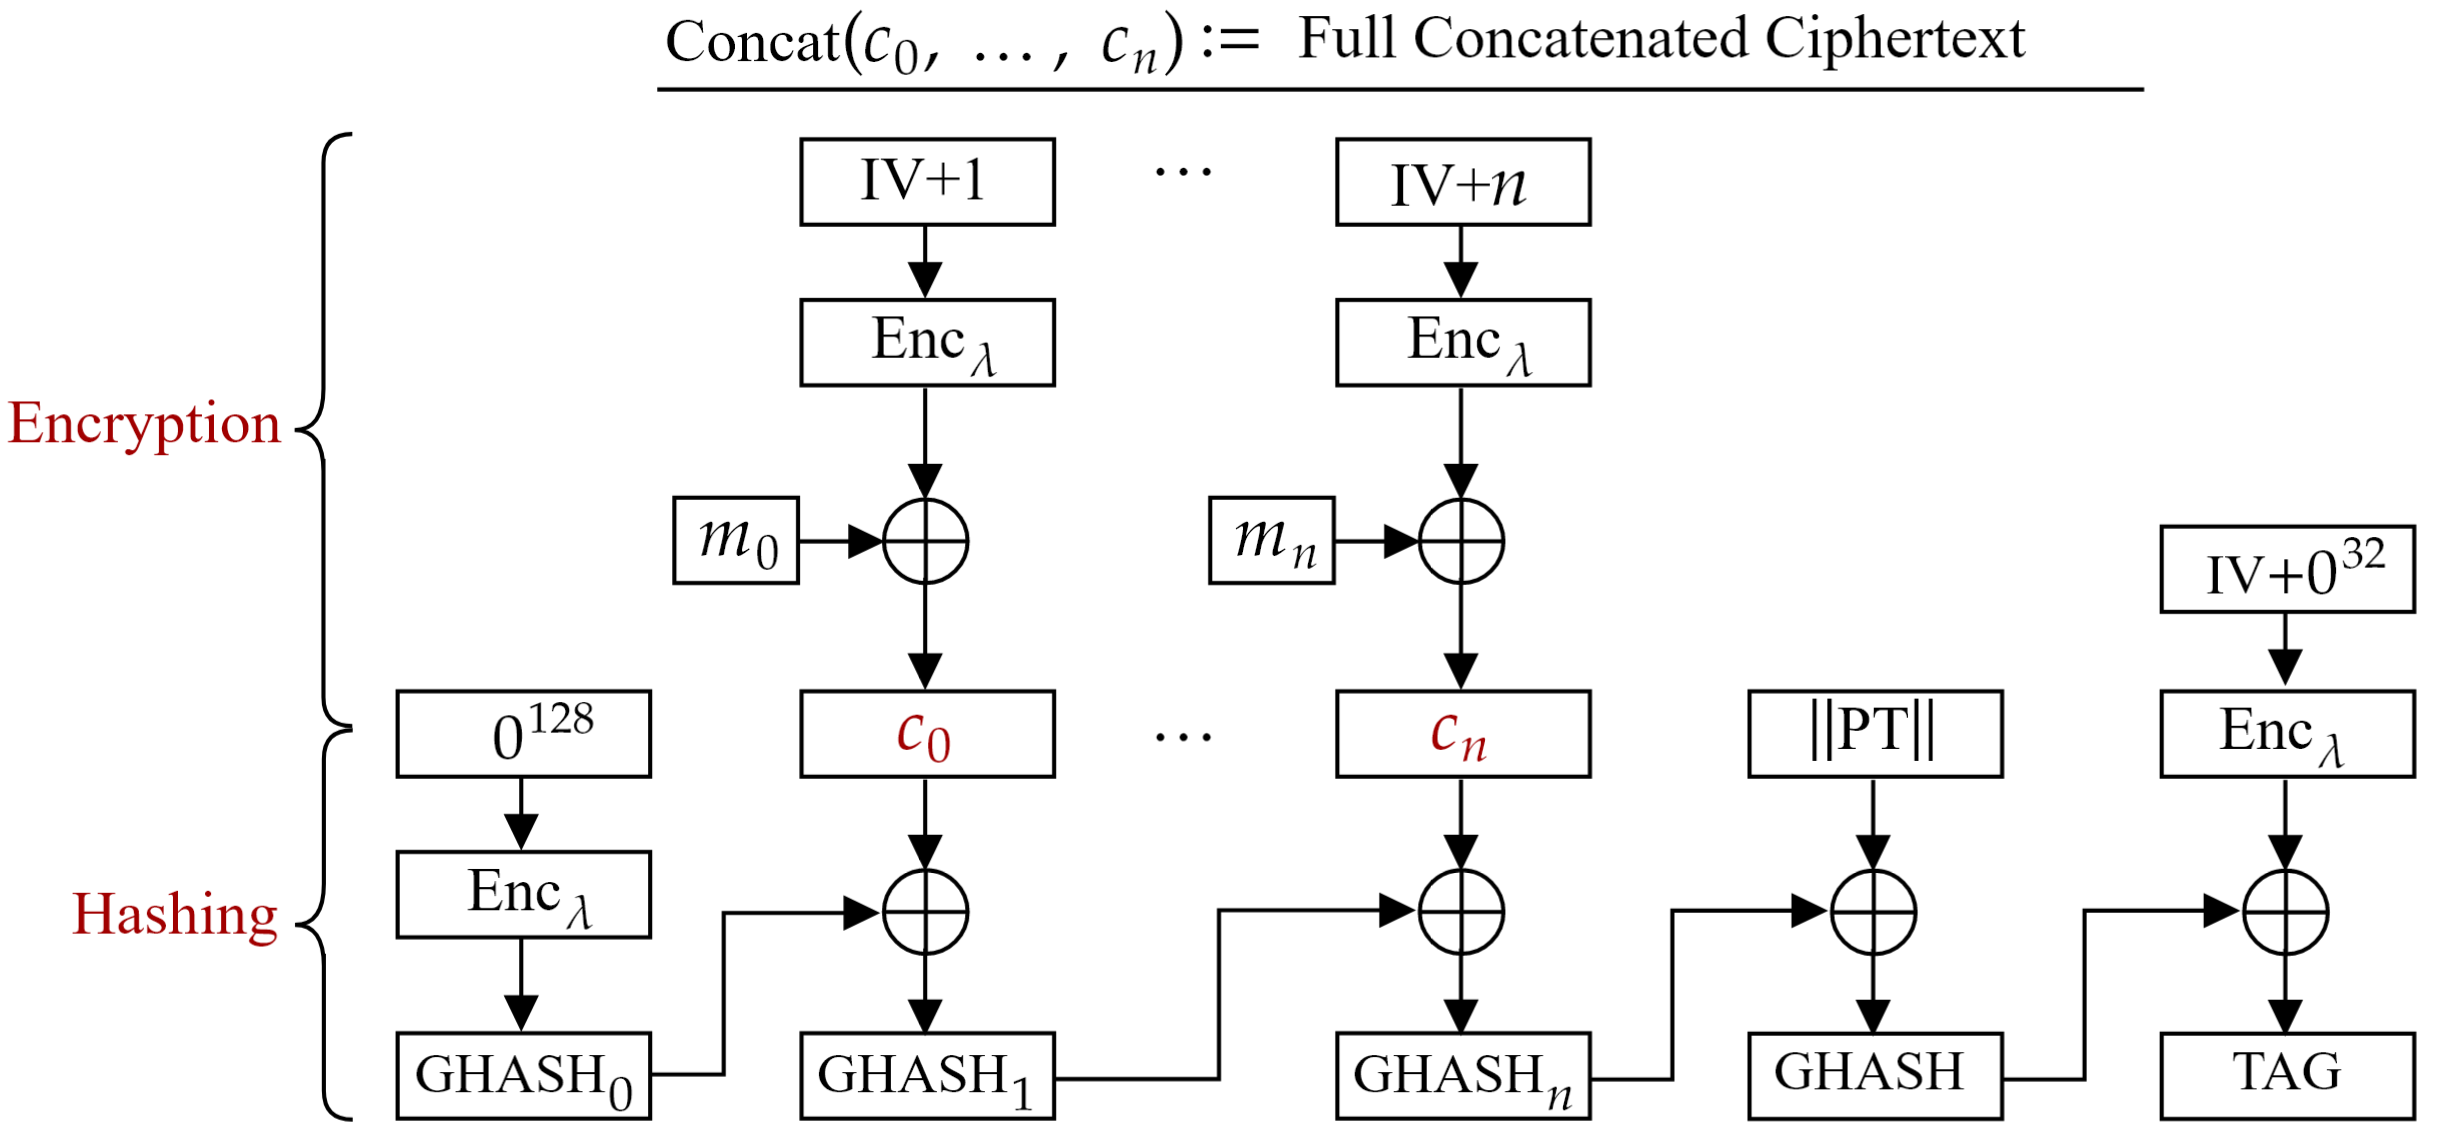
\includegraphics[width=1\textwidth]{Sections/sec/enc/semi.png}
    \caption{A semi complete GCM diagram (Encryption and Authentication), with AAD left out.}
    \label{fig:block_cipher}
\end{figure}
\noindent
\vfill
\begin{center}
    \textit{Continued on the next page.}
\end{center}
\vfill 
\newpage

\noindent
A full GCM diagram with AAD:
\begin{figure}[h!]
    \centering
    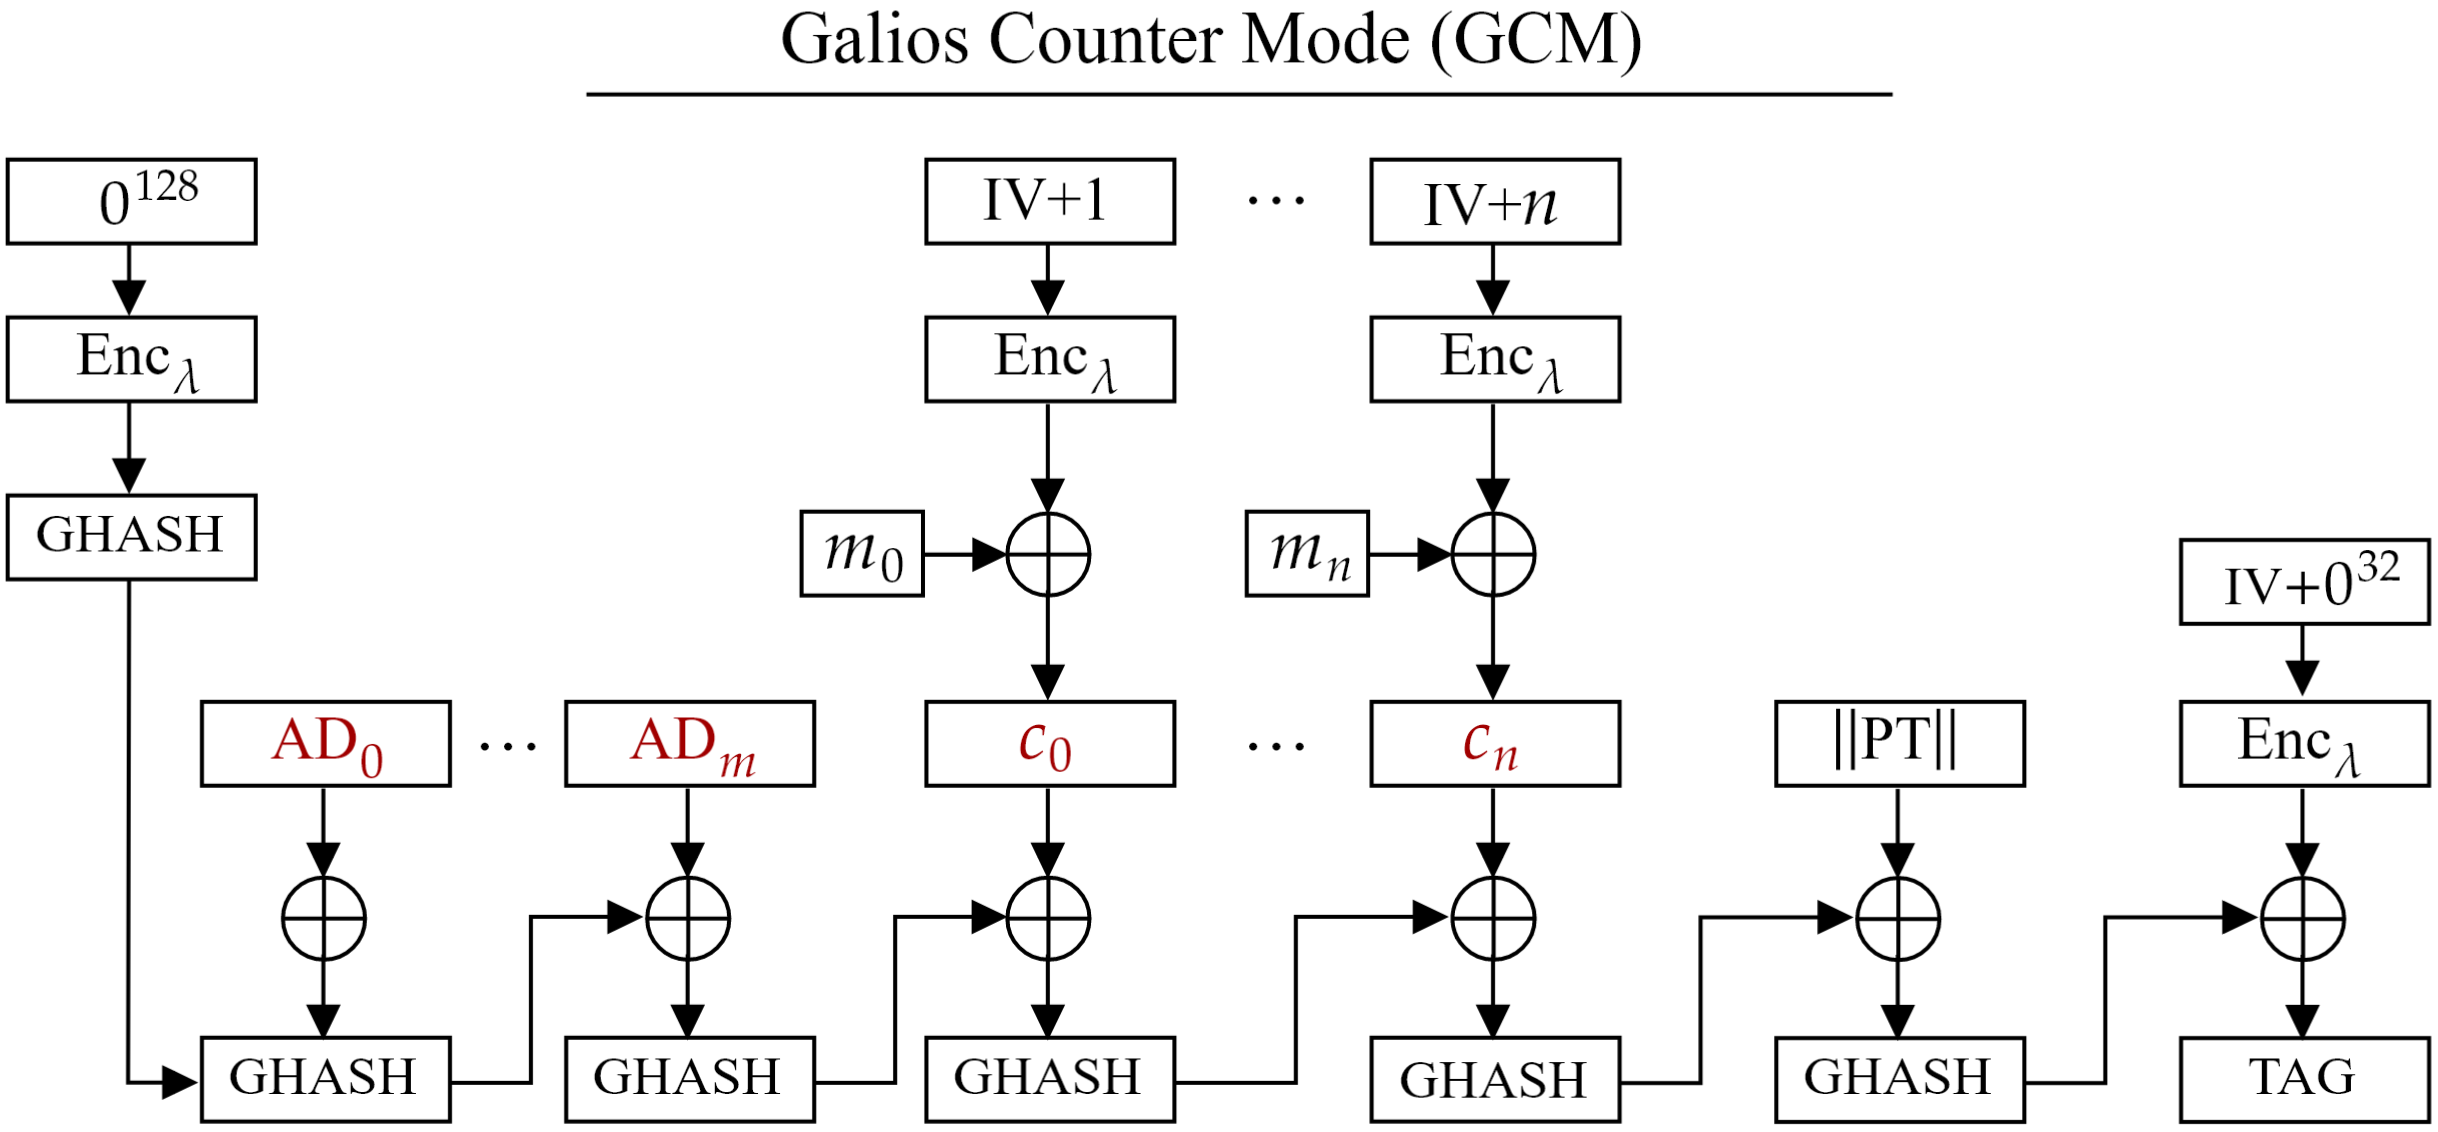
\includegraphics[width=1\textwidth]{Sections/sec/enc/gcm.png}
    \caption{A full GCM diagram: Encryption, Authentication, and unencrypted Additional Authenticated Data (AAD).}
    \label{fig:block_cipher}
\end{figure}


\noindent
\noindent
Now to discuss a possible shared key (symmetric key) algorithm usable Enc$_\lambda$ of GCM.
\begin{Def}[Advanced Encryption Standard (AES)]

    \label{theo:aes}
    During a worldwide competition in 2001, the National Institute of Standards and Technology (NIST) selected the Rijndael algorithm as the Advanced Encryption Standard (AES).
    AES is a symmetric key block cipher that encrypts plaintext (PT) in 128-bit blocks. AES works in rounds permuting the PT with partial keys generated from the initial key.
    \begin{itemize}
        \item \textbf{Key Expansion}: An initial key is expanded into a key schedule. These keys will be assigned to each round. 
        The rounds needed depend on the initial key size:
        \begin{enumerate}
            \item 128-bit key: 10 rounds, 11 keys.
            \item 192-bit key: 12 rounds, 13 keys.
            \item 256-bit key: 14 rounds, 15 keys.
        \end{enumerate}
        \item \textbf{Input Transformation}: The PT is transformed into a $4\times4$ matrix, called the \textbf{State}. The 
        state undergoes four main operations per round:
        \begin{enumerate}
            \item \textbf{SubBytes}: Each byte is substituted with a value from the S-Box.
            \item \textbf{ShiftRows}: Each row is shifted left by an offset.
            \item \textbf{MixColumns}: Each column is mixed with a fixed matrix.
            \item \textbf{AddRoundKey}: Each byte in the State is XORed with a sub-key. \hfill \cite{satish2024aes} \cite{nist_aes2001} \cite{brainkartAES2018}
        \end{enumerate}
    \end{itemize}

    
\end{Def}

\newpage 

\begin{Def}[Key Expansion]
    
        \label{theo:key_expansion}
        Key expansion, an AES process which takes a single key and expands it into multiple keys. The initial key 
        is broken up into 16-byte $4\times4$ matrices. Each column a \textbf{Word} (32-bits). The process follows 
        four main steps:
        \begin{center}
            \textbf{RotWord}$\rightarrow$\textbf{SubWord}$\rightarrow$\textbf{Rcon}$\rightarrow$\textbf{XOR}.\\
            (Rotate Word, Substitute Word, Round Constant, XOR)
        \end{center}
        
        \noindent
        This generates a \textbf{Sub-Key} for one round. Each round generates for the next round.
\end{Def}

\noindent
\textbf{AES Key Expansion:} Given the an initial 128-bit key, $\lambda_0$ ``my\_secret\_key001'':\\

\vspace{1em}

\hspace{-3em}
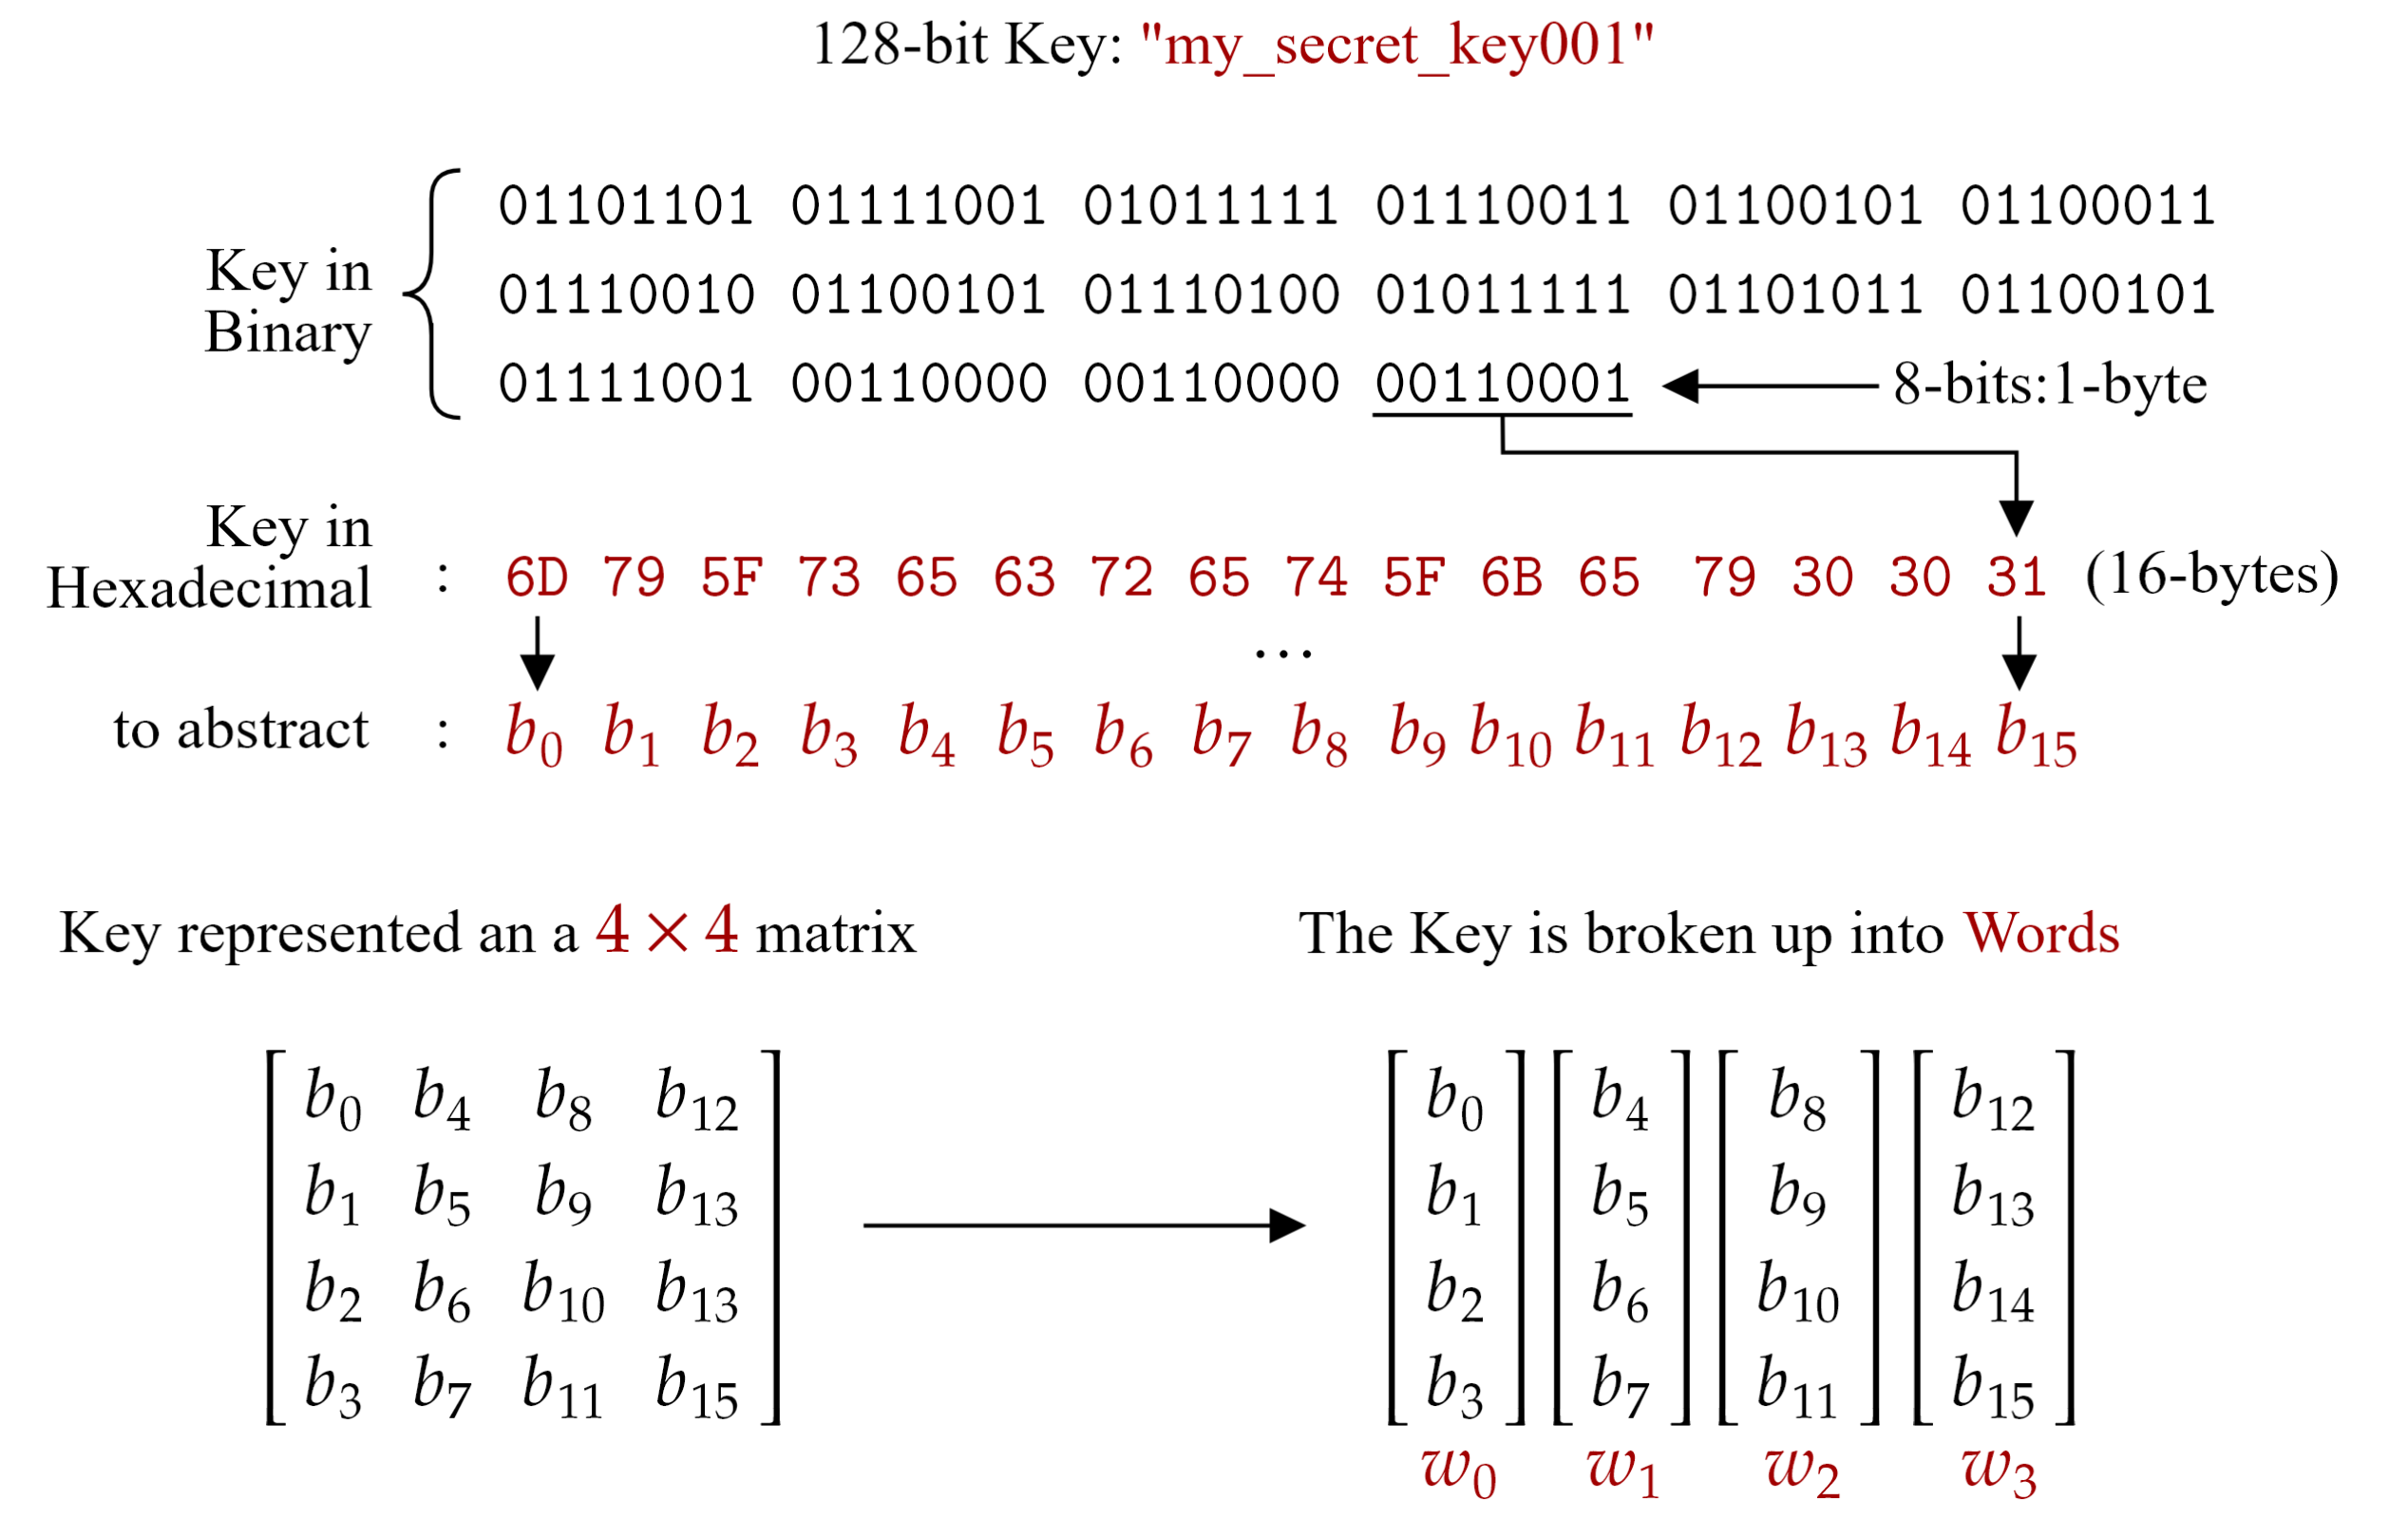
\includegraphics [width=1.1\textwidth]{Sections/sec/enc/aes/input.png}

\vspace{3em}
\noindent
These Words $w_0, w_1, w_2, w_3$ are the initial key. This will then generate the rest of the Words needed.
This first group is the first sub-key $s_0$ for the first round.

\newpage 

\hspace{-3em}
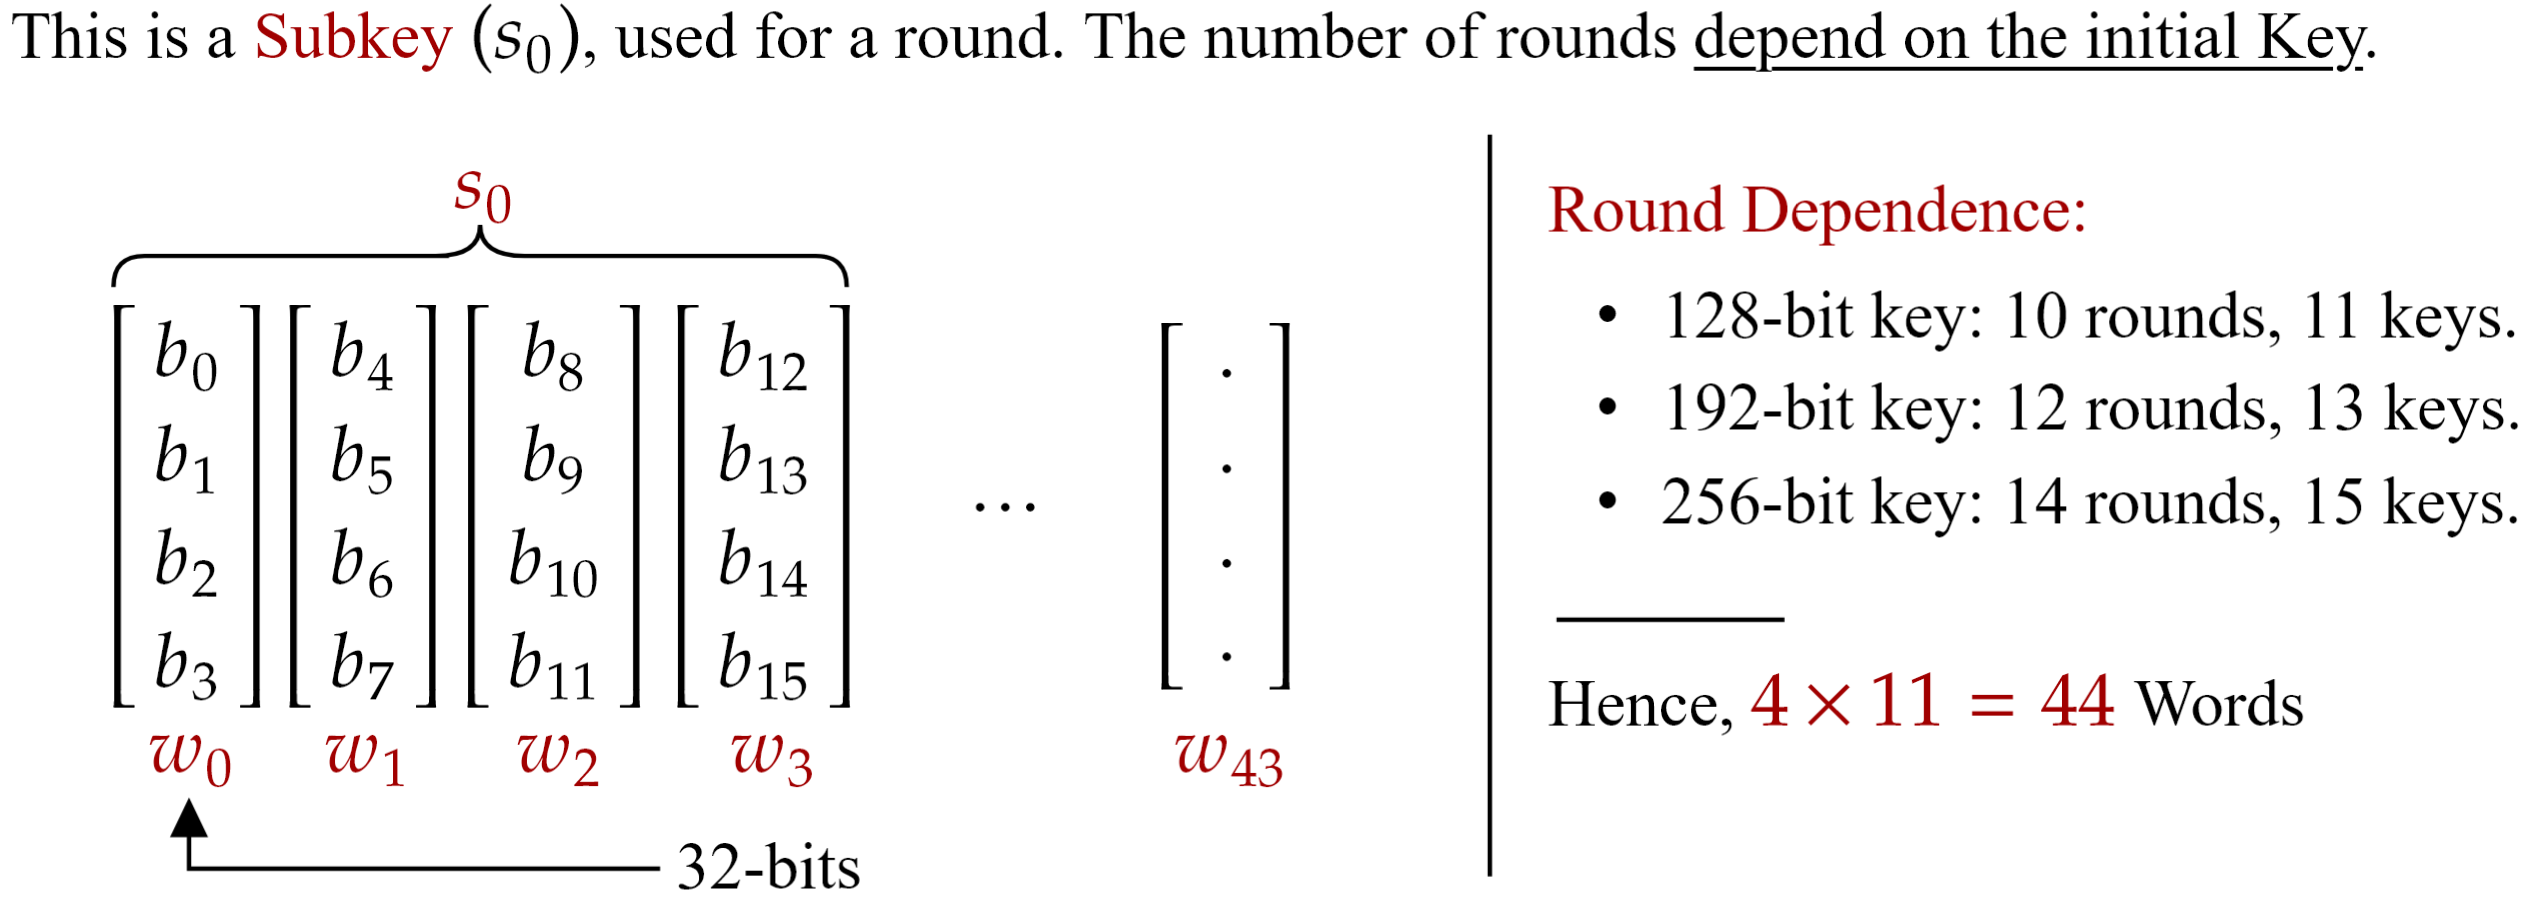
\includegraphics[width=1.1\textwidth]{Sections/sec/enc/aes/subkey.png}

\vspace{1em}
\noindent
\textcolor{gray}{Rounds depend on $\|\lambda_0\|$: 128-bits $\rightarrow$ 10 rounds, 192-bits $\rightarrow$ 12 rounds, 256-bits $\rightarrow$ 14 rounds.}

\vspace{1em}
\hspace{-3em}
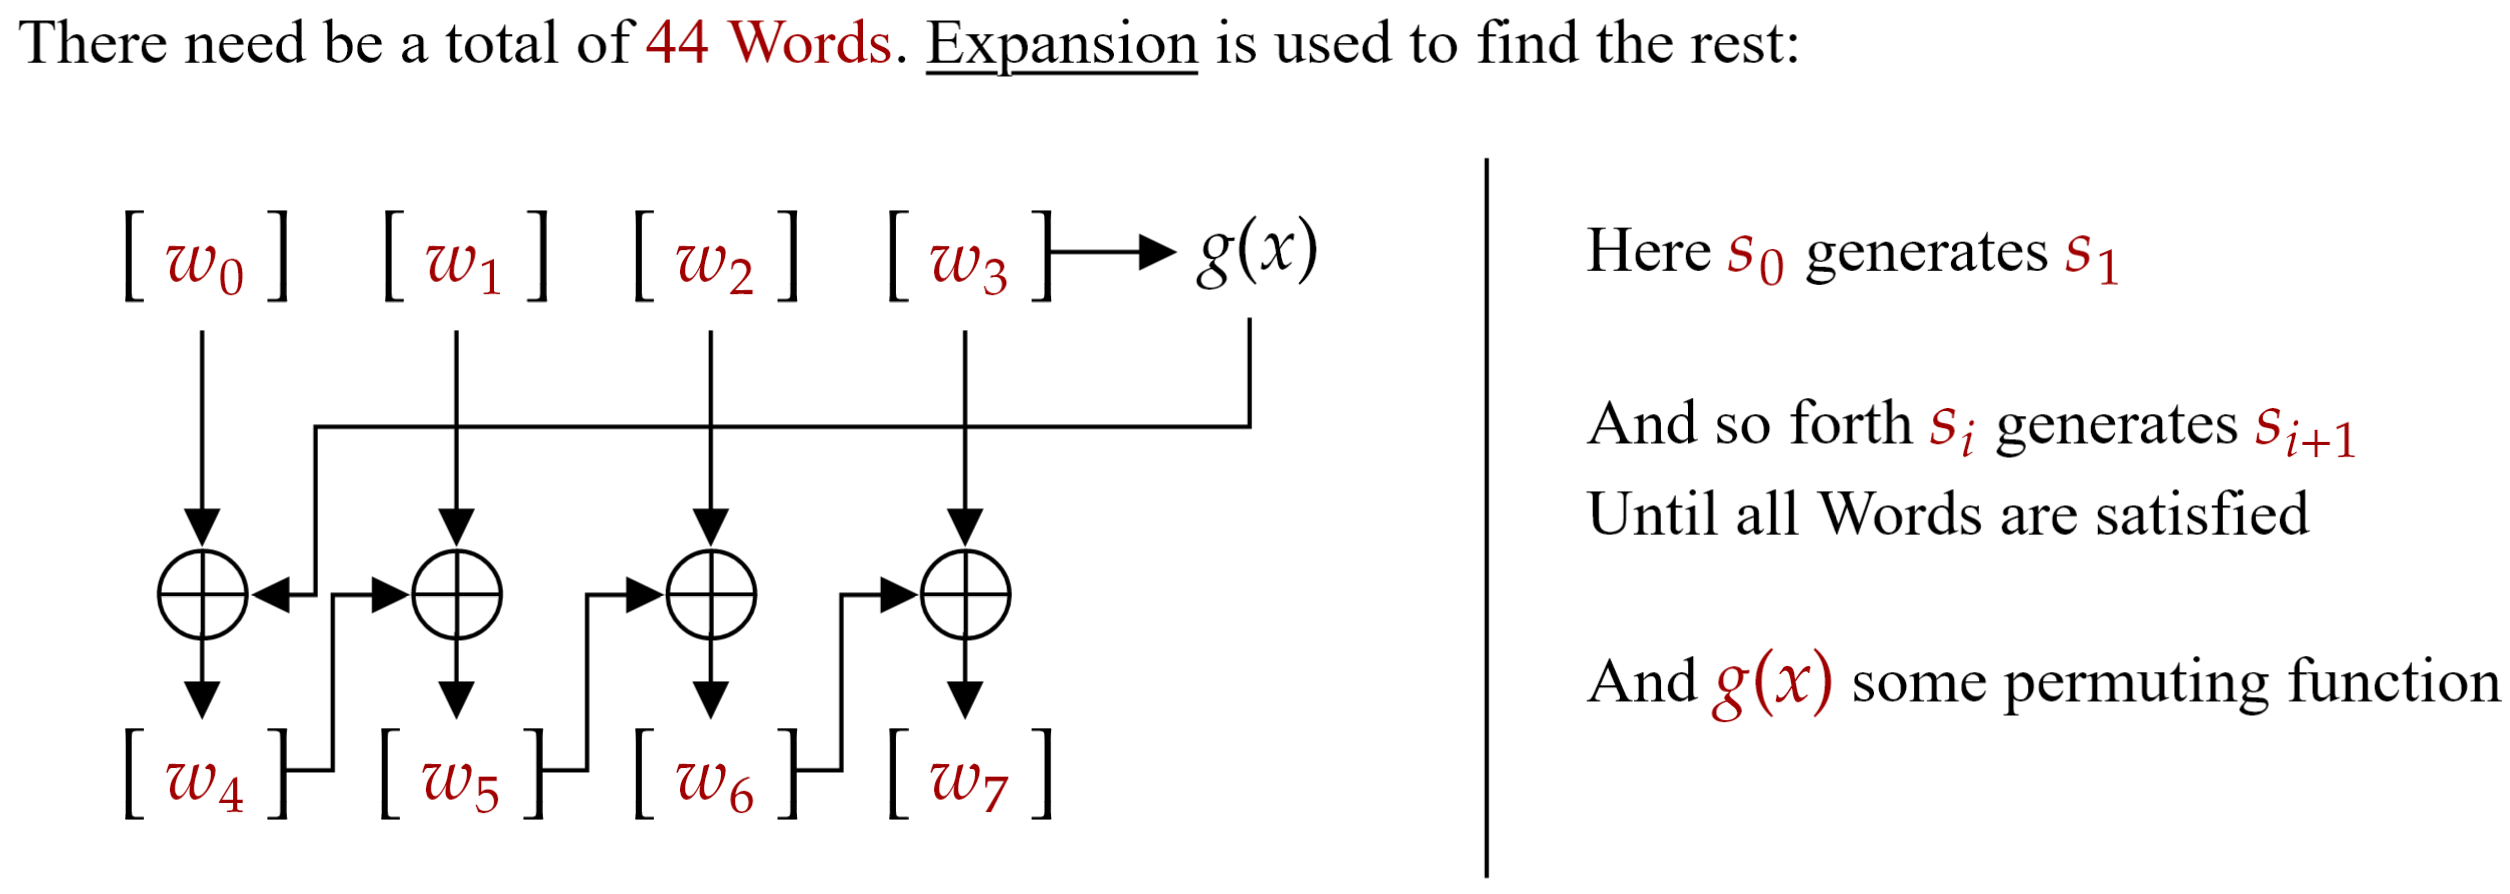
\includegraphics[width=1.1\textwidth]{Sections/sec/enc/aes/round_gen.png}

\noindent
\textcolor{gray}{The $g(x):=RotWord \circ SubWord \circ Rcon \circ XOR$, generating the next sub-key $s_1$.}

\vspace{1em}
\hspace{-3em}
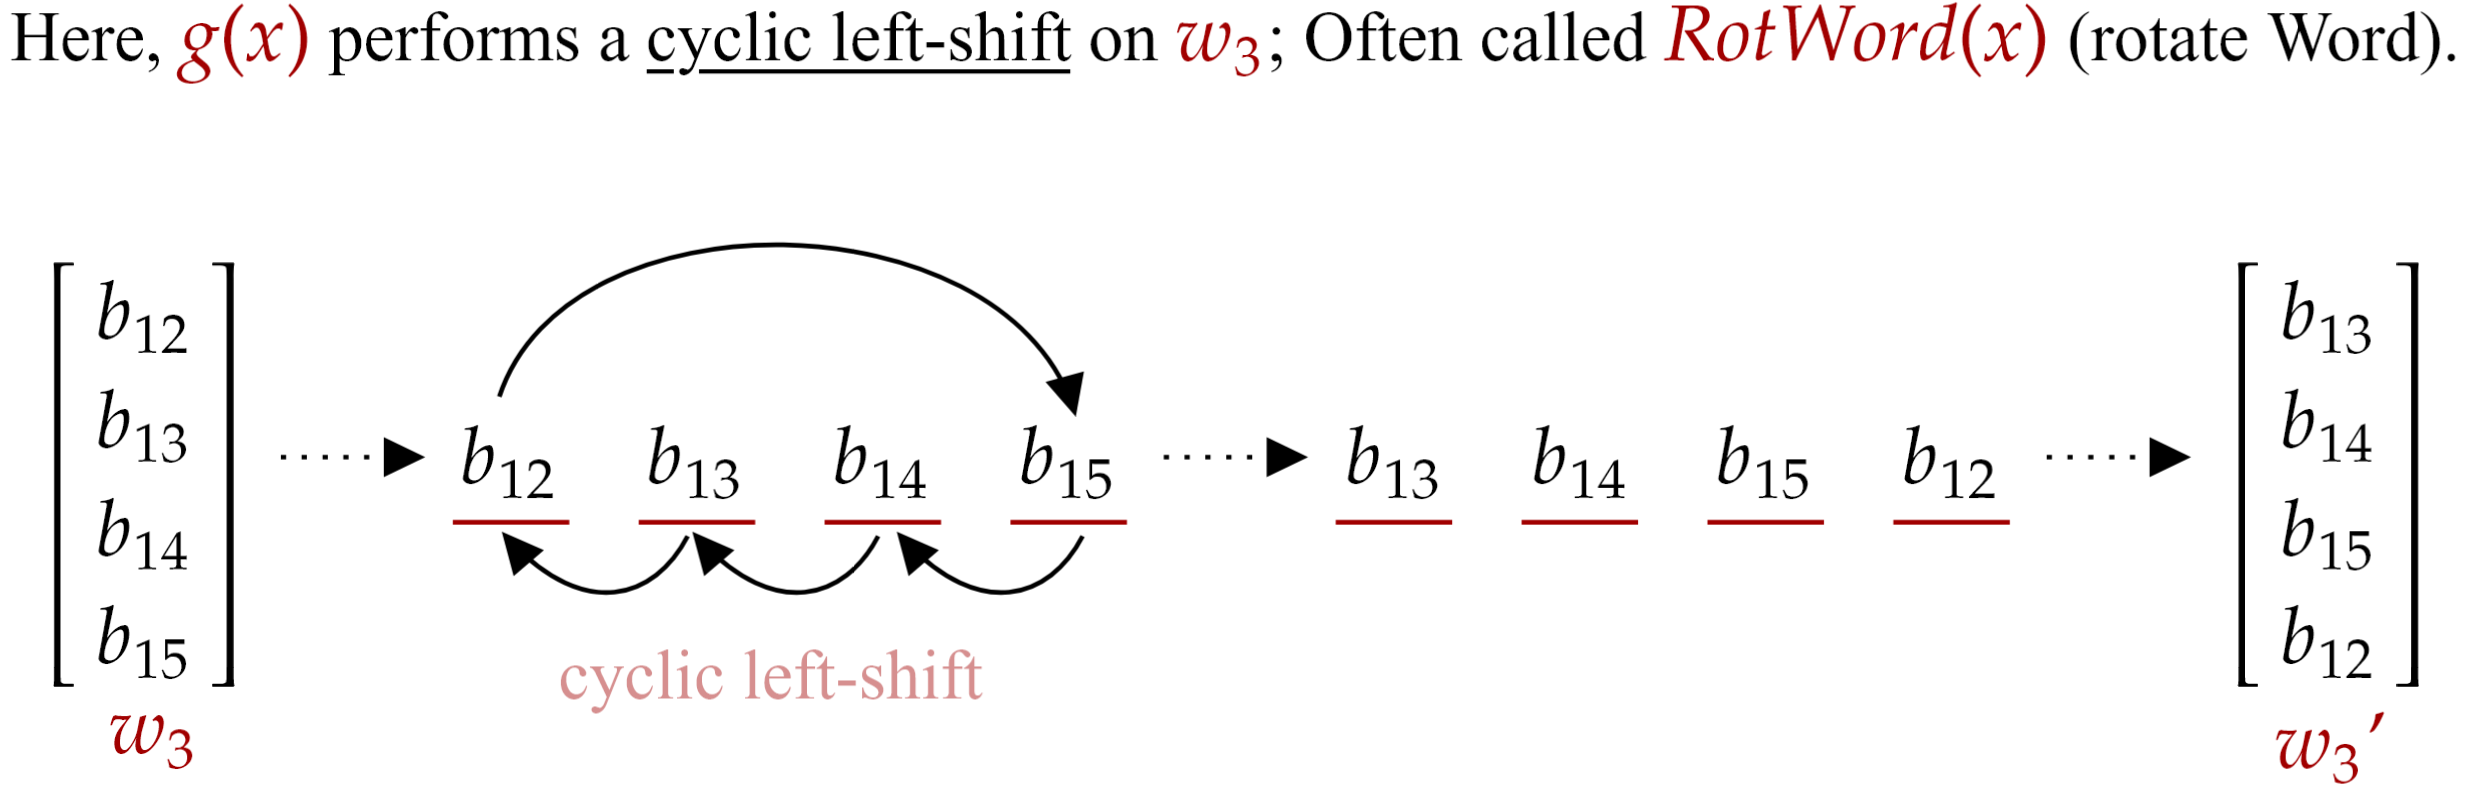
\includegraphics[width=1.1\textwidth]{Sections/sec/enc/aes/g_func.png}

\newpage
\noindent
\begin{Def}[Nibble]

    \label{theo:nibble}
    A \textbf{nibble} is a four-bit aggregation, referring to ``half a \textbf{byte}.'' A nibble splits 8-bits into two 4-bit values,
    the \textbf{upper nibble} and the \textbf{lower nibble}. E.g., given the hex value $0A$,
    the upper and lower nibble is $0$ and $A$ respectively.
\end{Def}
Now to quickly introduce some concepts needed for the AES borrowed from group theory.
\begin{Def}[Field]

    \label{def:field}
    A \textbf{field} is a set of elements equipped with two operations, addition and multiplication, such that the following properties hold:
    \begin{itemize}
        \item \textbf{Closure}: Adding or multiplying any two elements in the set remains in the set.
        \item \textbf{Associativity}: Addition and multiplication are associative.
        \item \textbf{Commutativity}: Addition and multiplication are commutative.
        \item \textbf{Identities}: There exist identity elements for addition (0) and multiplication (1).
        \item \textbf{Inverses}: Every element has an additive inverse (negative) and, except for 0, a multiplicative inverse (reciprocal).
        \item \textbf{Distributivity}: Multiplication distributes over addition.
    \end{itemize}

    \noindent
    E.g., The set of real numbers $\mathbb{R}$, with standard addition and multiplication, forms a field.
\end{Def}
\begin{theo}[Abel Ruffini Theorem]

    \label{theo:abel_ruffini}
    There is no general for solving polynomials of degree five or higher. Moreover,
    no formula is possible using these finite amount of: $+,-,\times,\div,\sqrt[n]{x}$.
\end{theo}

\noindent
This will play a key part in the AES algorithm, stopping attackers from reversing the encryption process.

\newpage

\begin{Def}[Galois Field $GF(2^8)$]

    \label{def:galois_field}
    The Galois Field $GF(2^8)$ is a finite field consisting of $2^8 = 256$ elements, where each element is an 8-bit binary value (a byte).
    Addition and multiplication in $GF(2^8)$ are defined modulo an irreducible polynomial of degree 8 over $GF(2)$ (the binary field).
    
    \noindent
    In AES, the irreducible polynomial used is:
    \[
    p(x) = x^8 + x^4 + x^3 + x + 1.
    \]
\end{Def}

\vspace{-1em}
\begin{Tip}
    To learn more consider this video on Galois Theory: \href{https://www.youtube.com/watch?v=1EWUsef0iFs}{``Why is there no quintic formula?''}
\end{Tip}


\begin{Def}[AES S-Box]

    \label{theo:aes_sbox}
    The AES S-Box is a substitution box used in the AES algorithm. It is a $16\times16$ matrix of 8-bit values. 
    The first column and row represent the upper and lower nibble of the input byte. E.g., given $C7$, column $c0$ and row $07$ intersect $c6$.
\end{Def}
\[
\begin{array}{|>{\columncolor[gray]{0.8}}c|c|*{15}{c|}}
\hline
    \rowcolor{black} & \textcolor{white}{00} & \textcolor{white}{01} & \textcolor{white}{02} & \textcolor{white}{03} & \textcolor{white}{04} & \textcolor{white}{05} & \textcolor{white}{06} & \textcolor{white}{07} & \textcolor{white}{08} & \textcolor{white}{09} & \textcolor{white}{0a} & \textcolor{white}{0b} & \textcolor{white}{0c} & \textcolor{white}{0d} & \textcolor{white}{0e} & \textcolor{white}{0f} \\
\hline
00 & 63 & 7c & 77 & 7b & f2 & 6b & 6f & c5 & 30 & 01 & 67 & 2b & fe & d7 & ab & 76 \\
10 & ca & 82 & c9 & 7d & fa & 59 & 47 & f0 & ad & d4 & a2 & af & 9c & a4 & 72 & c0 \\
20 & b7 & fd & 93 & 26 & 36 & 3f & f7 & cc & 34 & a5 & e5 & f1 & 71 & d8 & 31 & 15 \\
30 & 04 & c7 & 23 & c3 & 18 & 96 & 05 & 9a & 07 & 12 & 80 & e2 & eb & 27 & b2 & 75 \\
40 & 09 & 83 & 2c & 1a & 1b & 6e & 5a & a0 & 52 & 3b & d6 & b3 & 29 & e3 & 2f & 84 \\
50 & 53 & d1 & 00 & ed & 20 & fc & b1 & 5b & 6a & cb & be & 39 & 4a & 4c & 58 & cf \\
60 & d0 & ef & aa & fb & 43 & 4d & 33 & 85 & 45 & f9 & 02 & 7f & 50 & 3c & 9f & a8 \\
70 & 51 & a3 & 40 & 8f & 92 & 9d & 38 & f5 & bc & b6 & da & 21 & 10 & ff & f3 & d2 \\
80 & cd & 0c & 13 & ec & 5f & 97 & 44 & 17 & c4 & a7 & 7e & 3d & 64 & 5d & 19 & 73 \\
90 & 60 & 81 & 4f & dc & 22 & 2a & 90 & 88 & 46 & ee & b8 & 14 & de & 5e & 0b & db \\
a0 & e0 & 32 & 3a & 0a & 49 & 06 & 24 & 5c & c2 & d3 & ac & 62 & 91 & 95 & e4 & 79 \\
b0 & e7 & c8 & 37 & 6d & d5 & 4e & a9 & 6c & 56 & f4 & ea & 65 & 7a & ae & 08 & ba \\
c0 & ba & 78 & 25 & 2e & 1c & a6 & b4 & c6 & e8 & dd & 74 & 1f & 4b & bd & 8b & 8a \\
d0 & 70 & 3e & b5 & 66 & 48 & 03 & f6 & 0e & 61 & 35 & 57 & 89 & 86 & c1 & 1d & 9e \\
e0 & e1 & f8 & 98 & 11 & 69 & d9 & 8e & 94 & 9b & 1e & 87 & e9 & ce & 55 & 28 & df \\
f0 & 8c & a1 & 89 & 0d & bf & e6 & 42 & 68 & 41 & 99 & 2d & 0f & b0 & 54 & bb & 16 \\
\hline
\end{array}
\]

\newpage 

\noindent
For reference, previous figures are shown again.

\begin{center}
    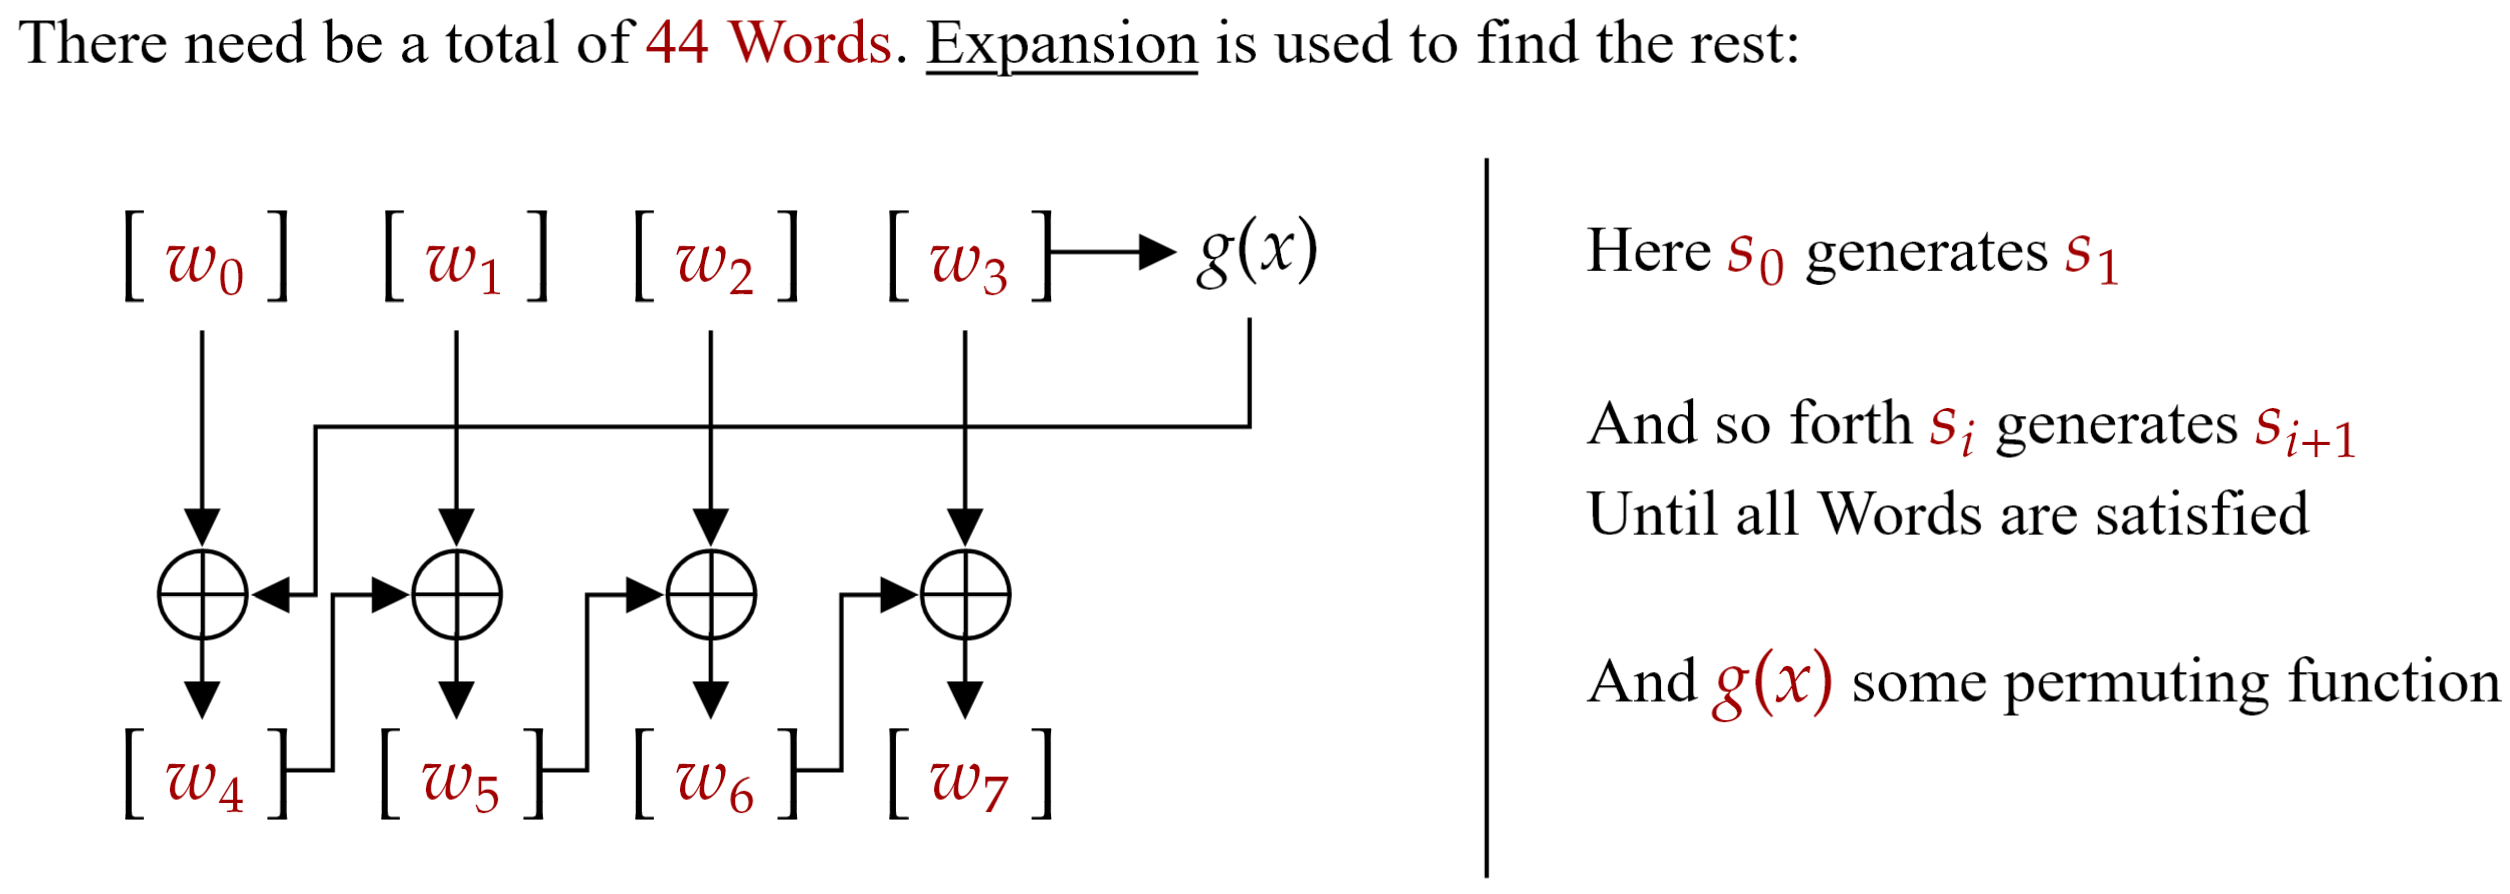
\includegraphics[width=.8\textwidth]{Sections/sec/enc/aes/round_gen.png}

    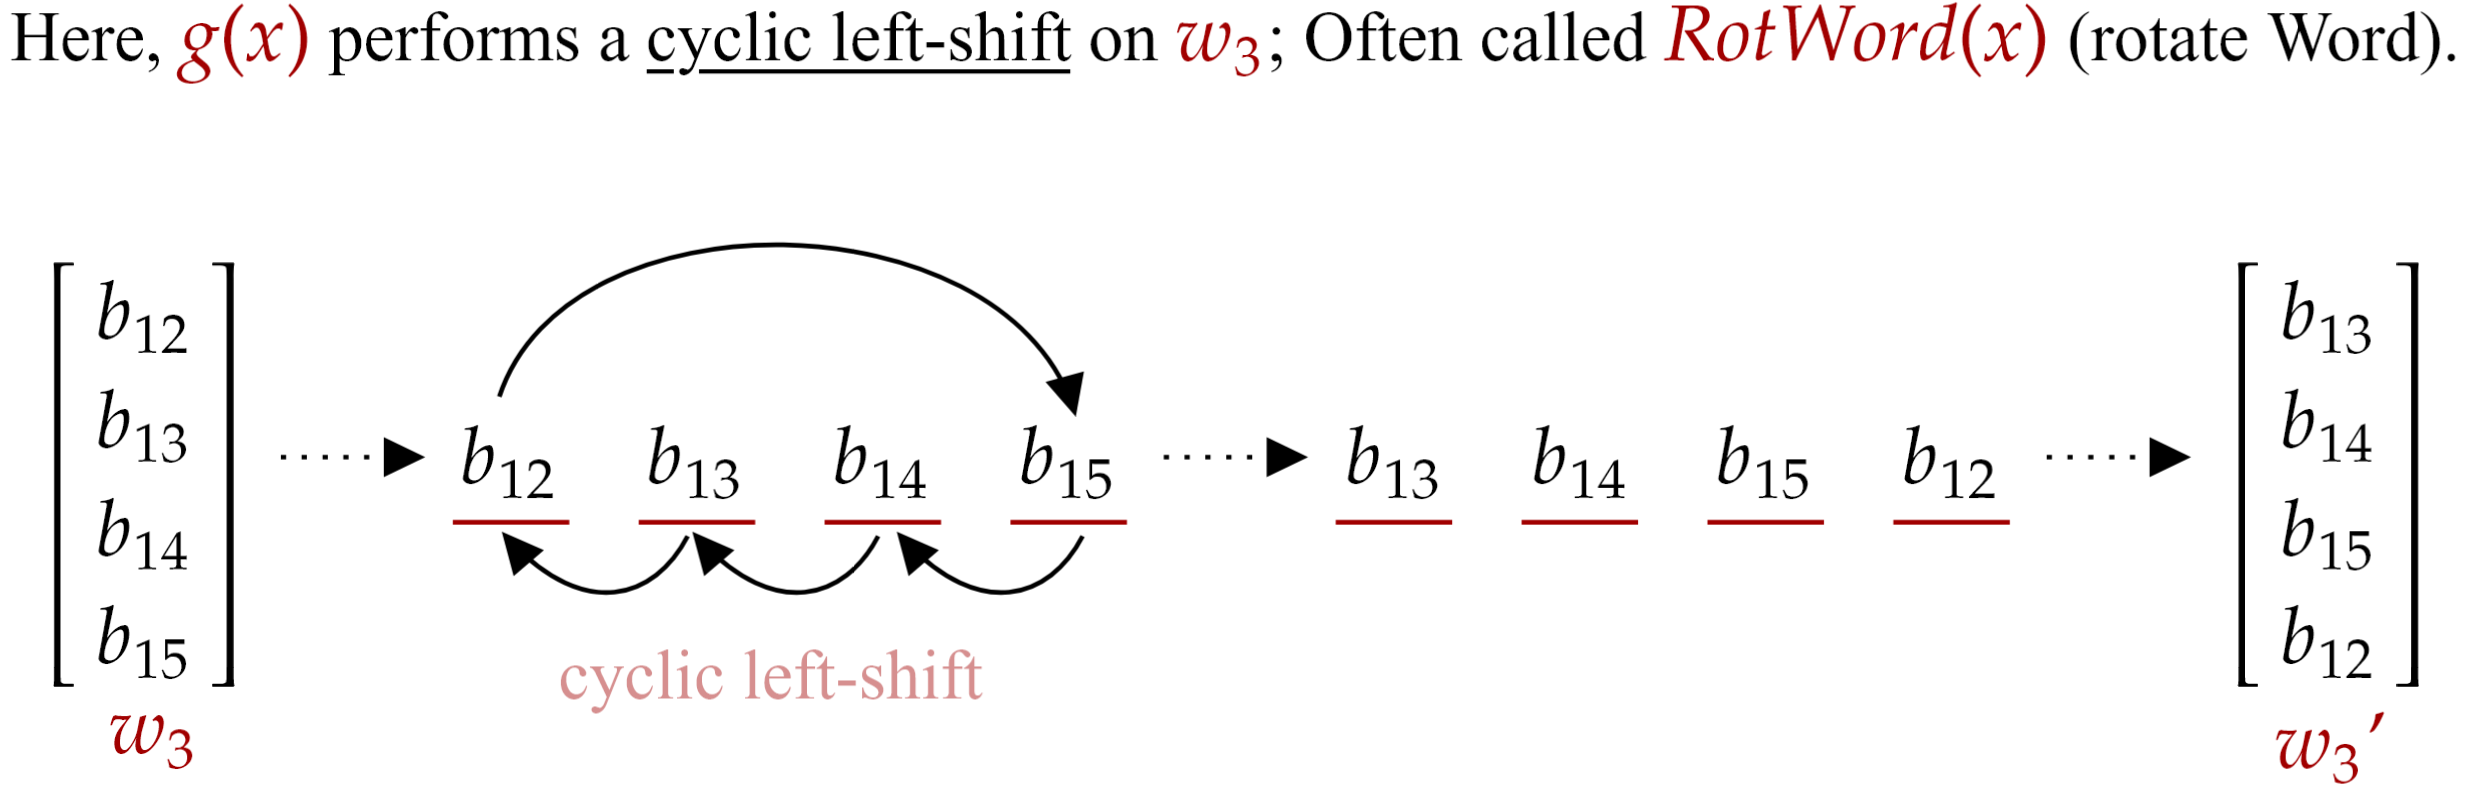
\includegraphics[width=.8\textwidth]{Sections/sec/enc/aes/g_func.png}

\end{center}

\vspace{1em}
\noindent

\hspace{-3em}
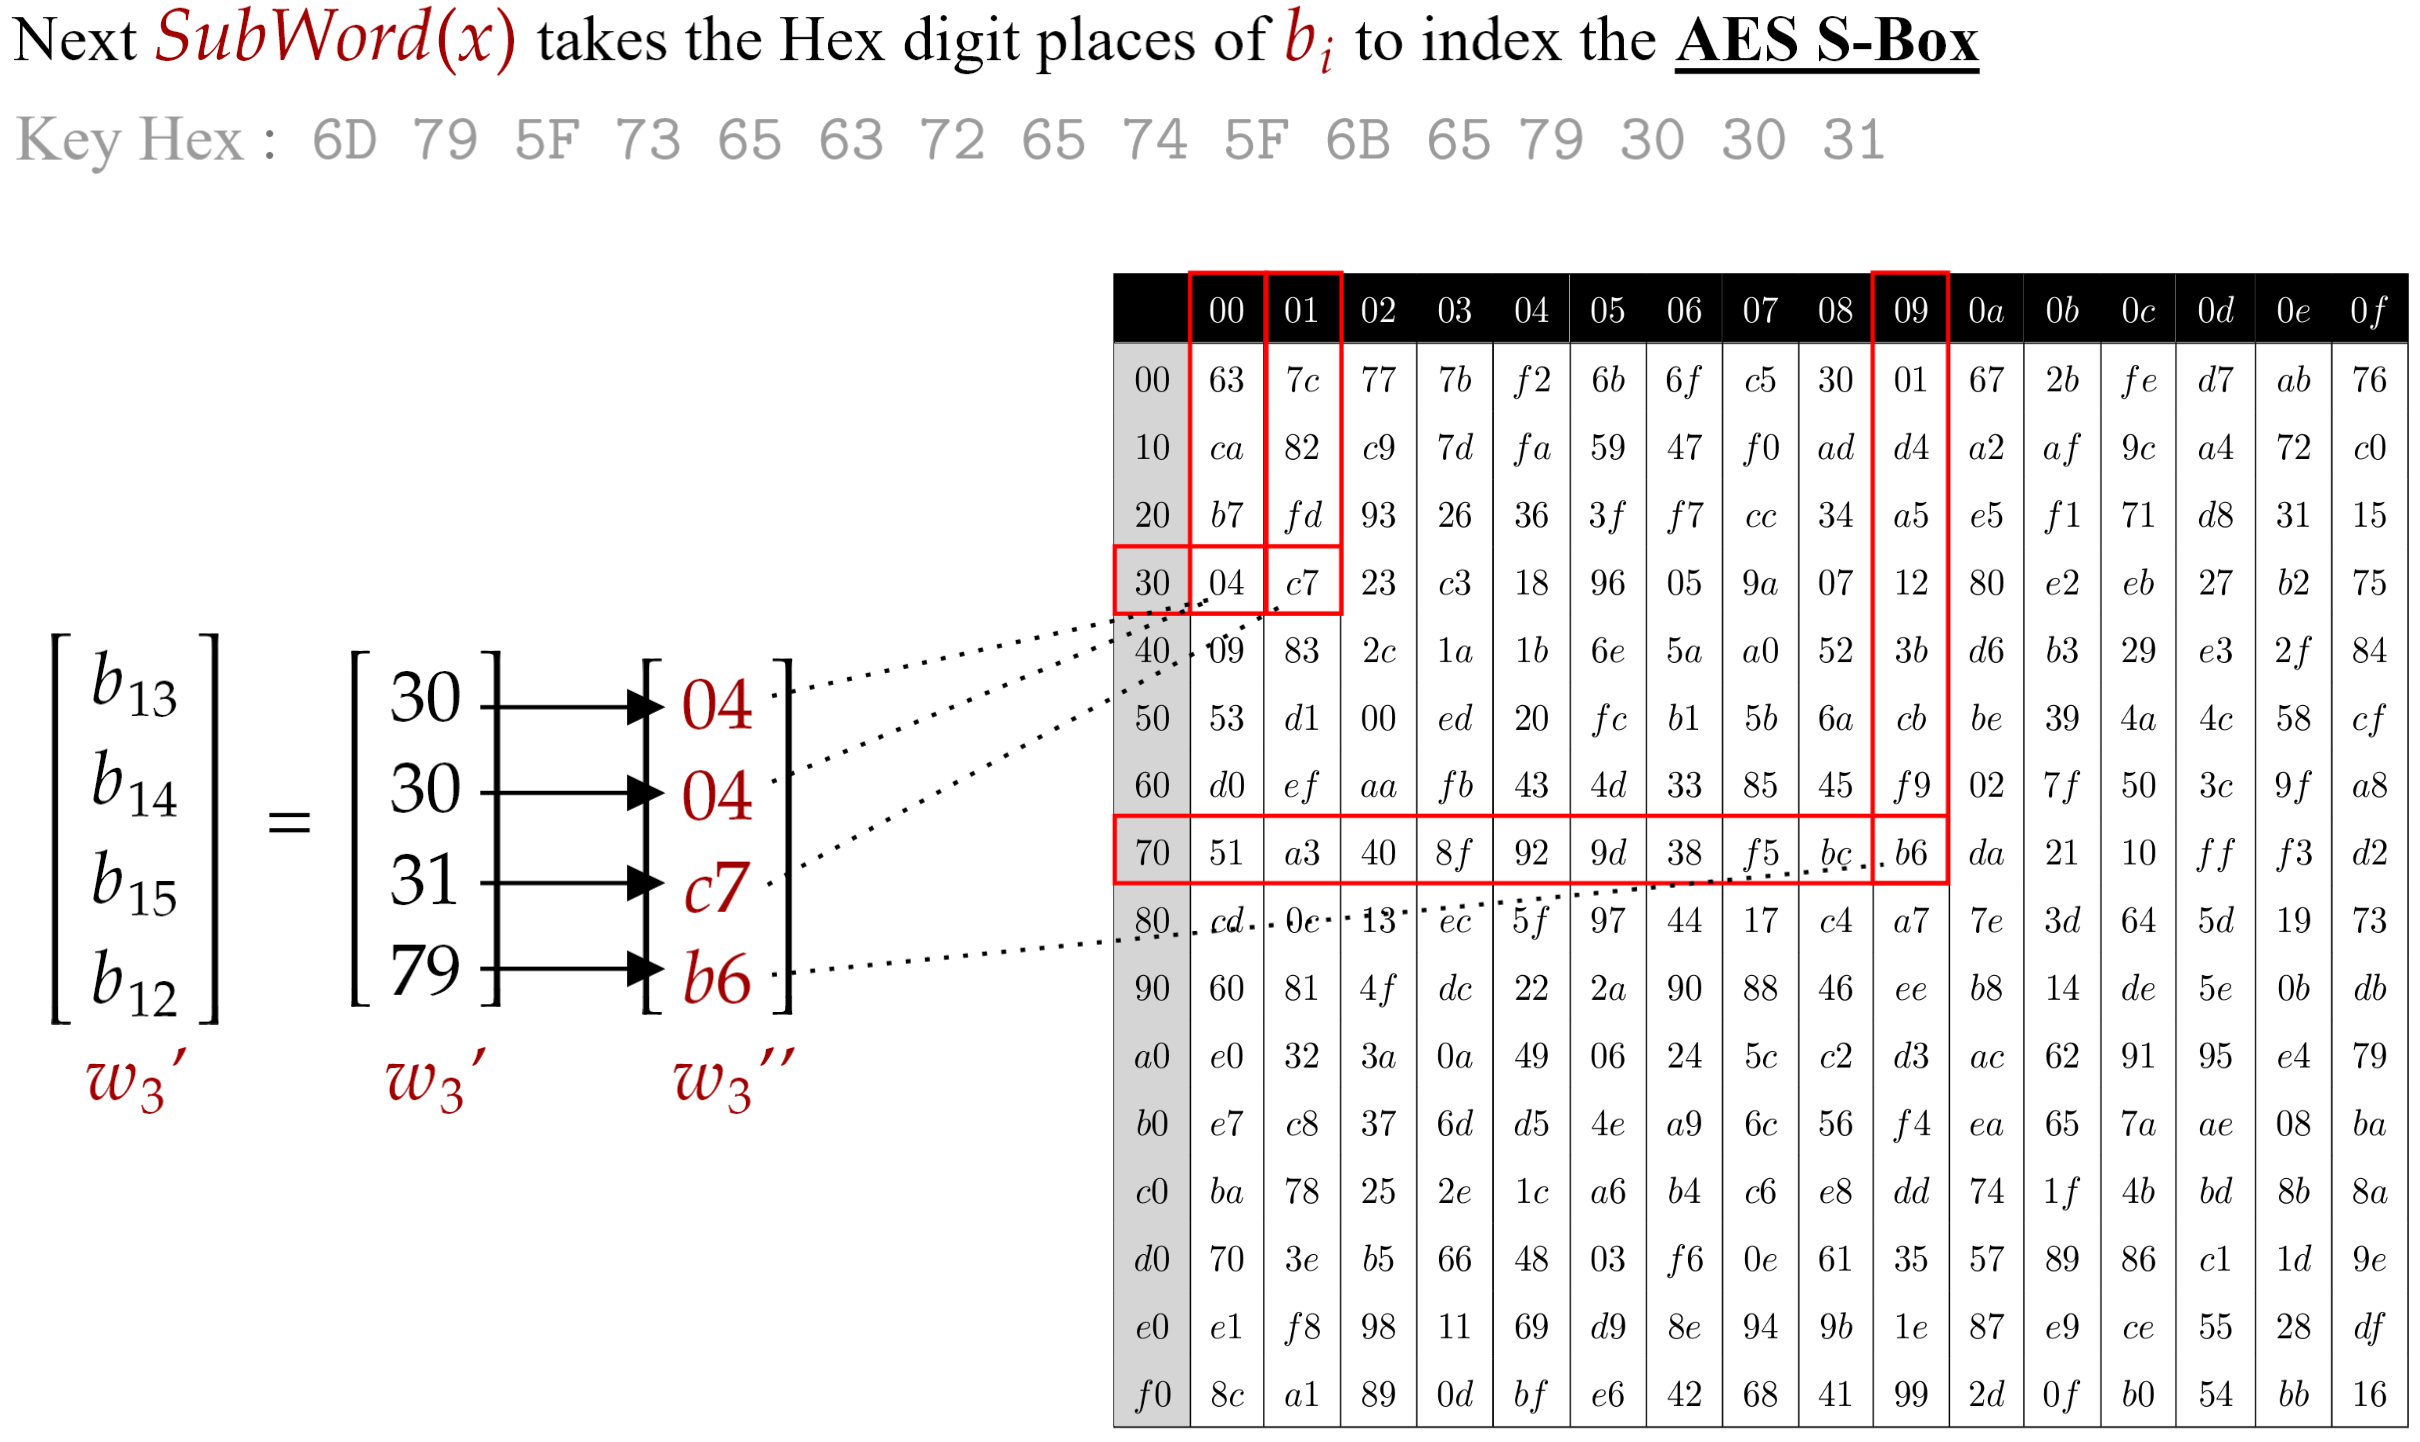
\includegraphics[width=1.1\textwidth]{Sections/sec/enc/aes/sub_word.png}

\newpage 

\begin{Def}[Round Constants]

    \label{theo:round_constants}
    Round constants take the output of $SubWord(x)$ and XOR the first byte with a constant value.
    The constant value, denoted $Rcon[j]$, is derived from powers of 2 in the Galois Field $GF(2^8)$, where the irreducible polynomial is $x^8 + x^4 + x^3 + x + 1$.

    Each round constant ensures the uniqueness of round keys during the AES key expansion process, introducing nonlinearity and breaking symmetry between rounds.
\end{Def}

\begin{table}[h!]
    \centering
    \renewcommand{\arraystretch}{1.4}
    \begin{tabular}{|c|c|c|}
    \hline
    \textbf{Round (i)} & \textbf{\textit{Rcon} Value} & \textbf{Power of 2 in GF(2\textsuperscript{8})} \\
    \hline
    1  & 0x01 00 00 00 & $2^0 = 1$     \\
    2  & 0x02 00 00 00 & $2^1 = 2$     \\
    3  & 0x04 00 00 00 & $2^2 = 4$     \\
    4  & 0x08 00 00 00 & $2^3 = 8$     \\
    5  & 0x10 00 00 00 & $2^4 = 16$    \\
    6  & 0x20 00 00 00 & $2^5 = 32$    \\
    7  & 0x40 00 00 00 & $2^6 = 64$    \\
    8  & 0x80 00 00 00 & $2^7 = 128$   \\
    9  & 0x1B 00 00 00 & $2^8 \, \text{mod poly}$ \\
    10 & 0x36 00 00 00 & $2^9 \, \text{mod poly}$ \\
    \hline
    \end{tabular}
    \caption{Round Constants, where poly:= $x^8 + x^4 + x^3 + x + 1$.}
    \label{tab:rcon-values}
\end{table}


\hspace{-3em}
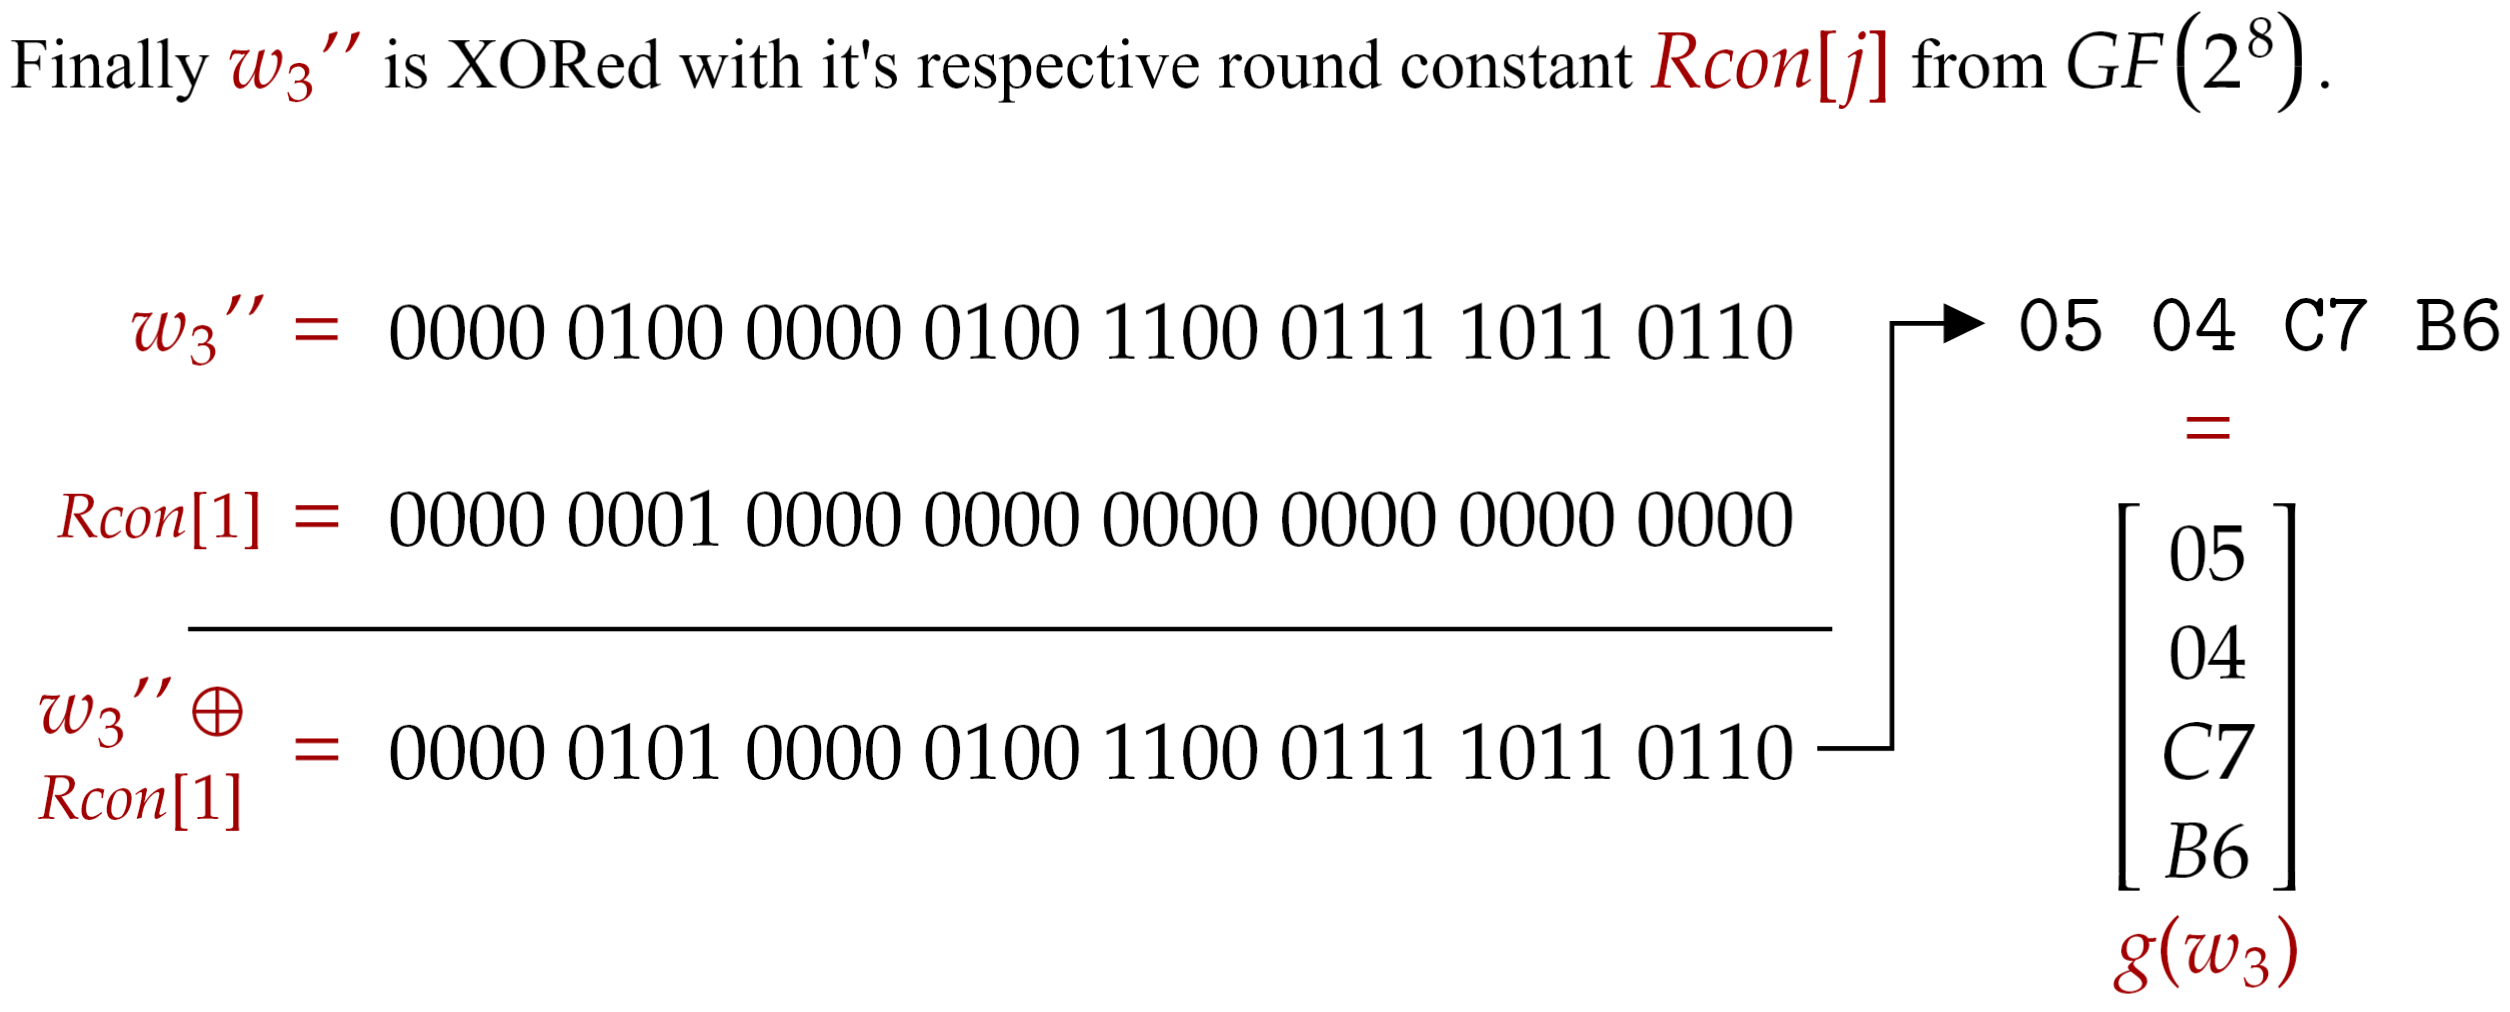
\includegraphics[width=1\textwidth]{Sections/sec/enc/aes/rcon.png}

\newpage 

\noindent
All together:\\

\hspace{-2em}
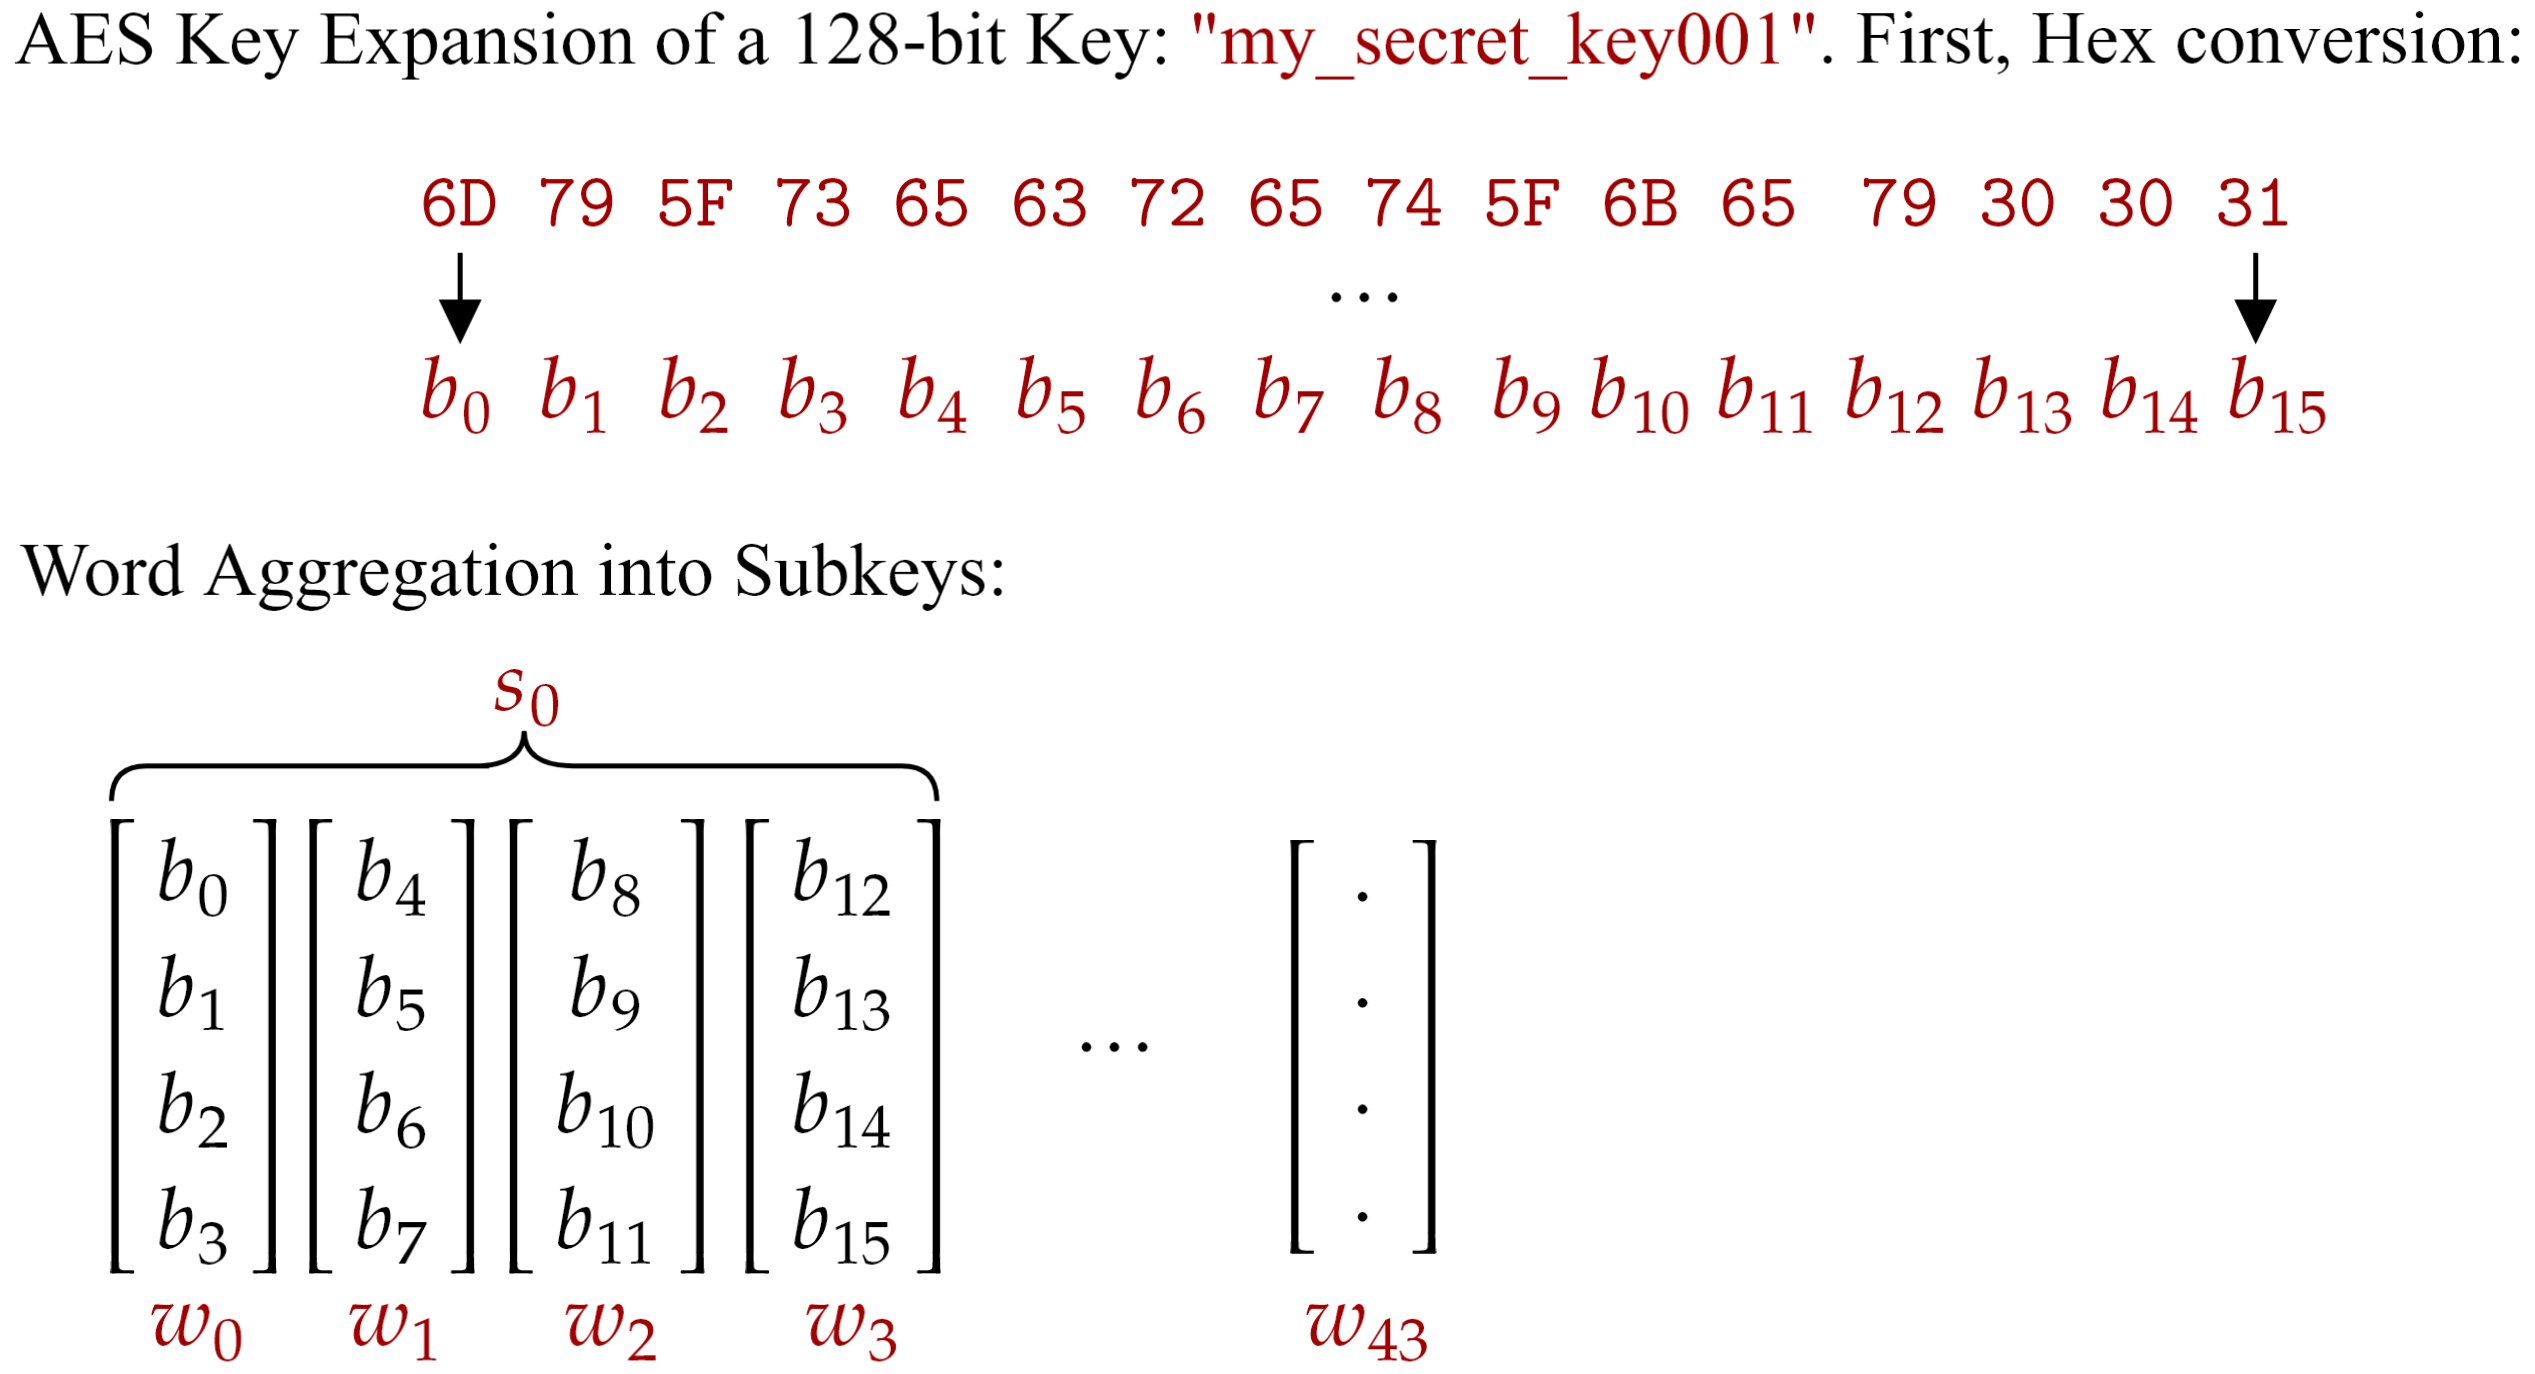
\includegraphics[width=1\textwidth]{Sections/sec/enc/aes/recap1.png}

\hspace{-2em}
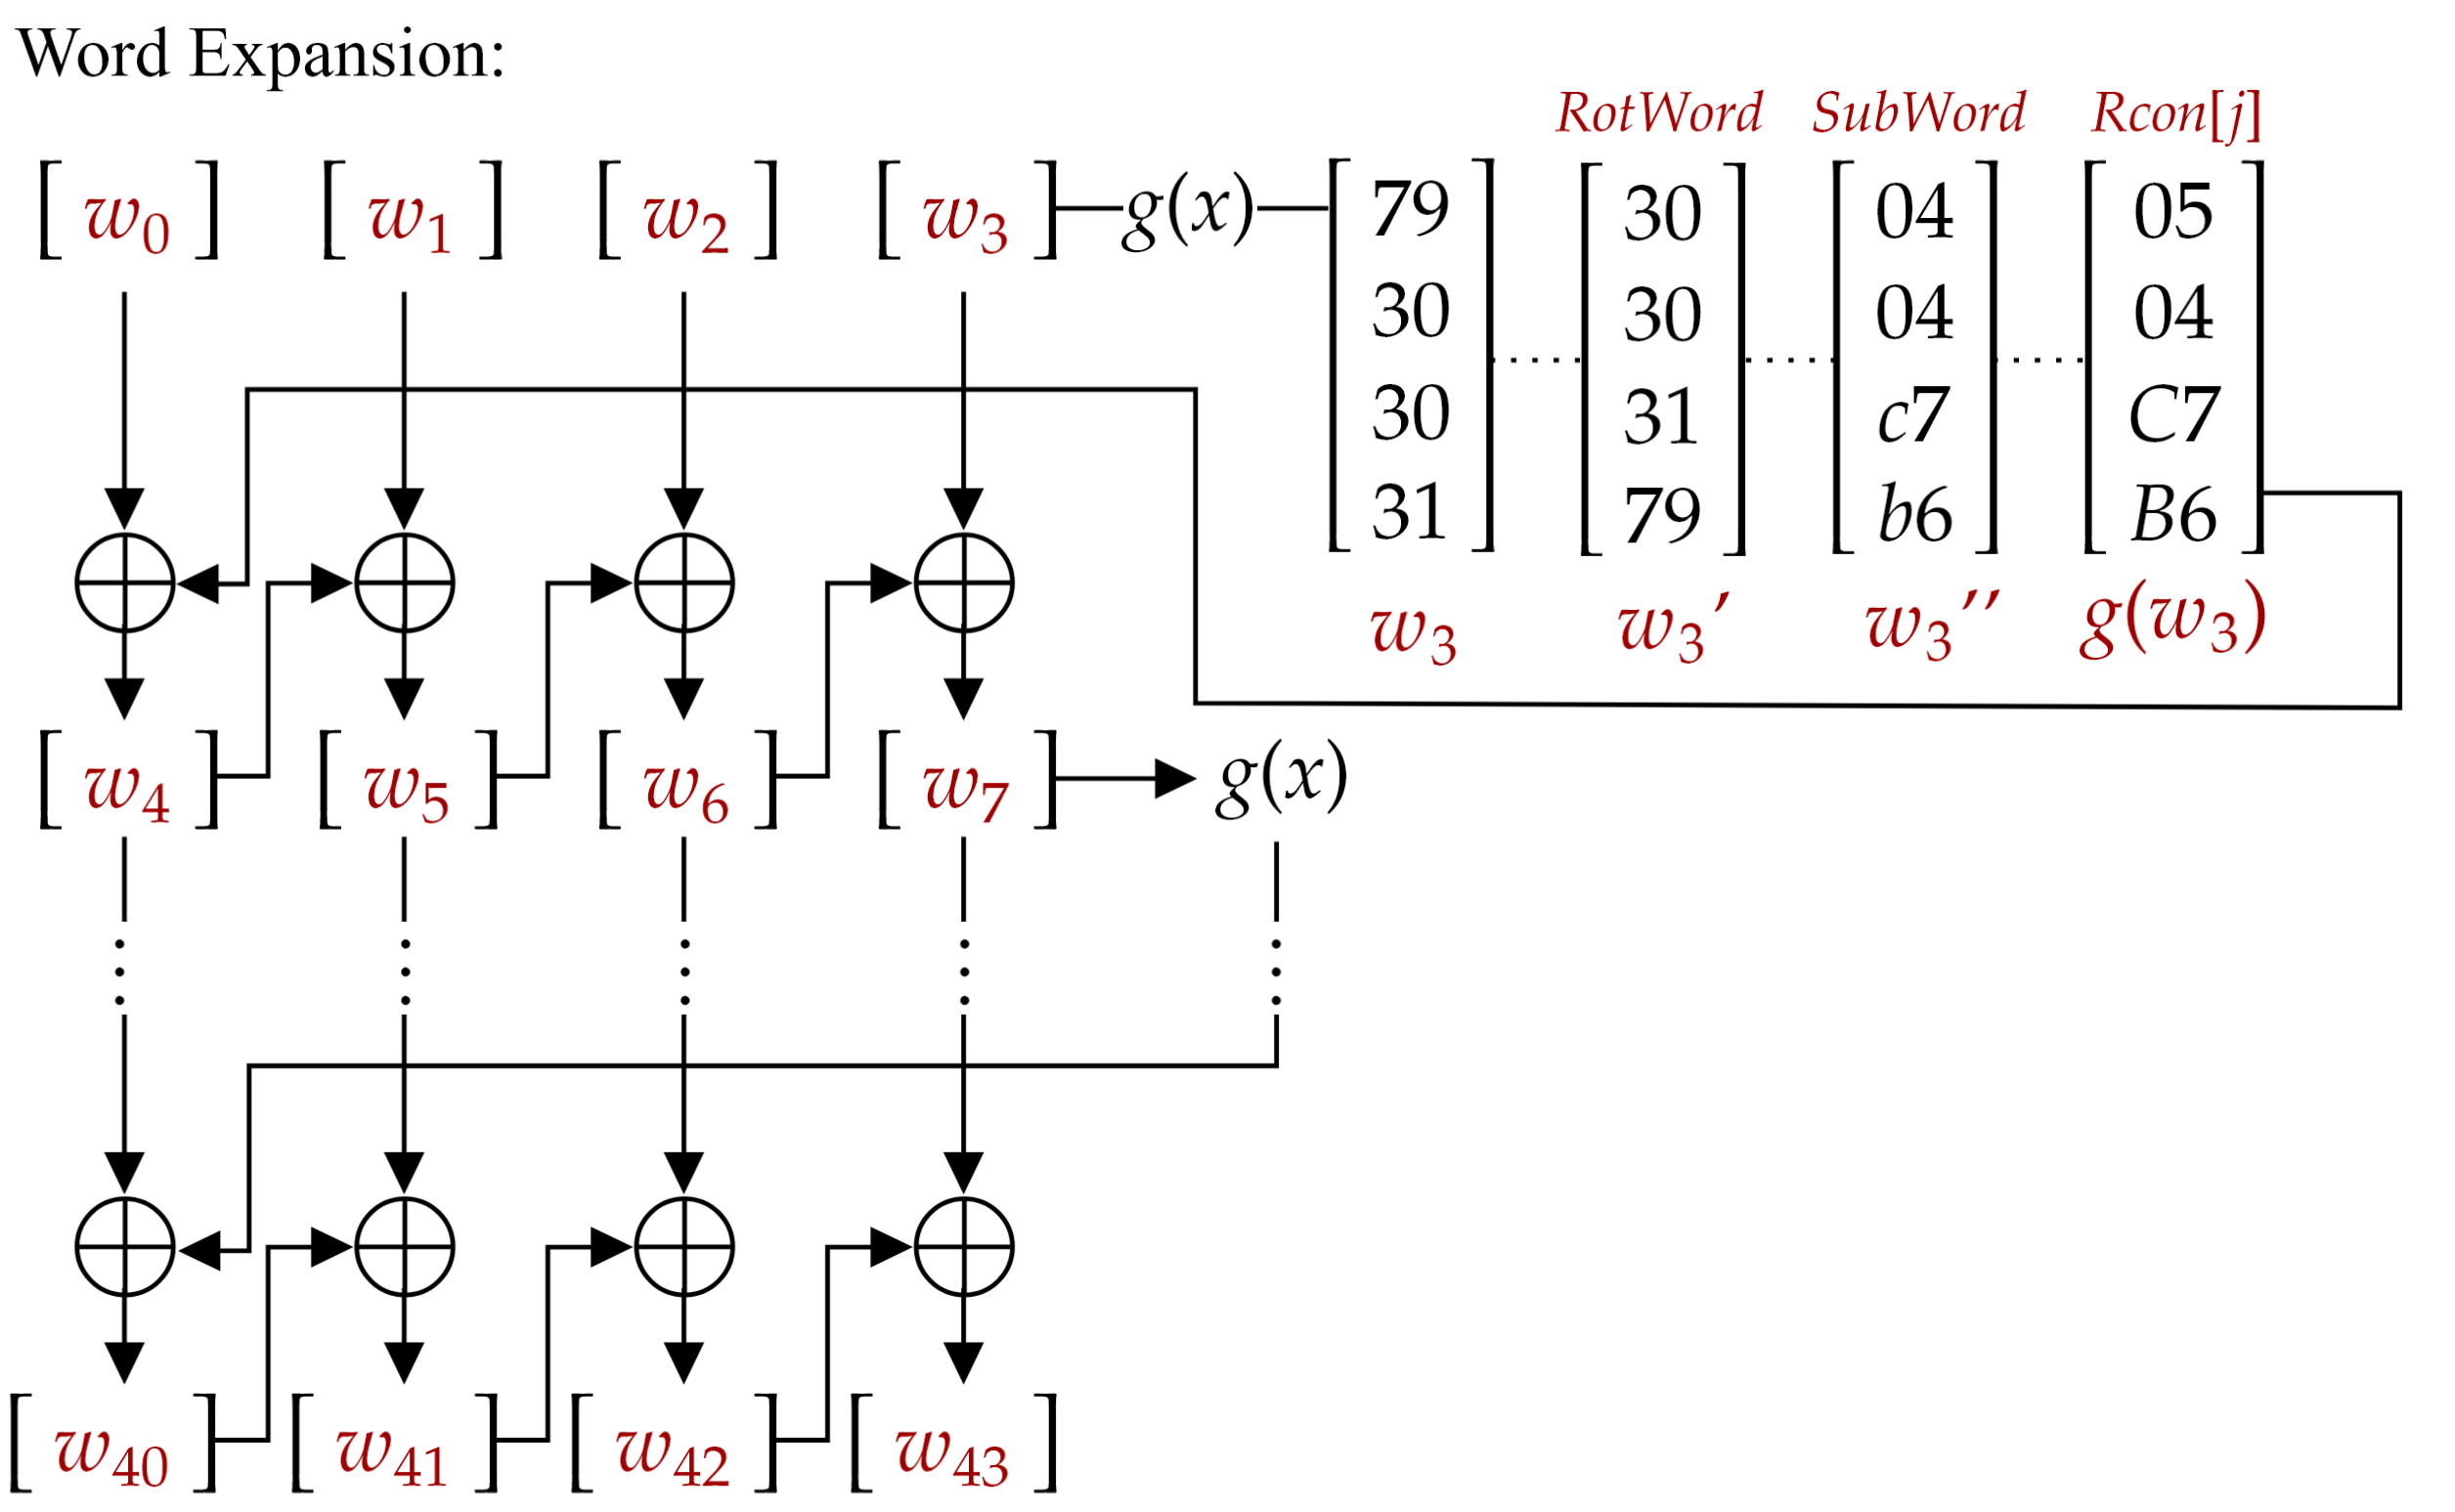
\includegraphics[width=1\textwidth]{Sections/sec/enc/aes/recap2.png}

\vspace{1em}
\noindent
This is AES Key Expansion.

\newpage 

\noindent
Now to discuss the AES encryption process.\\
\vspace{1em}
\hspace{-3em}
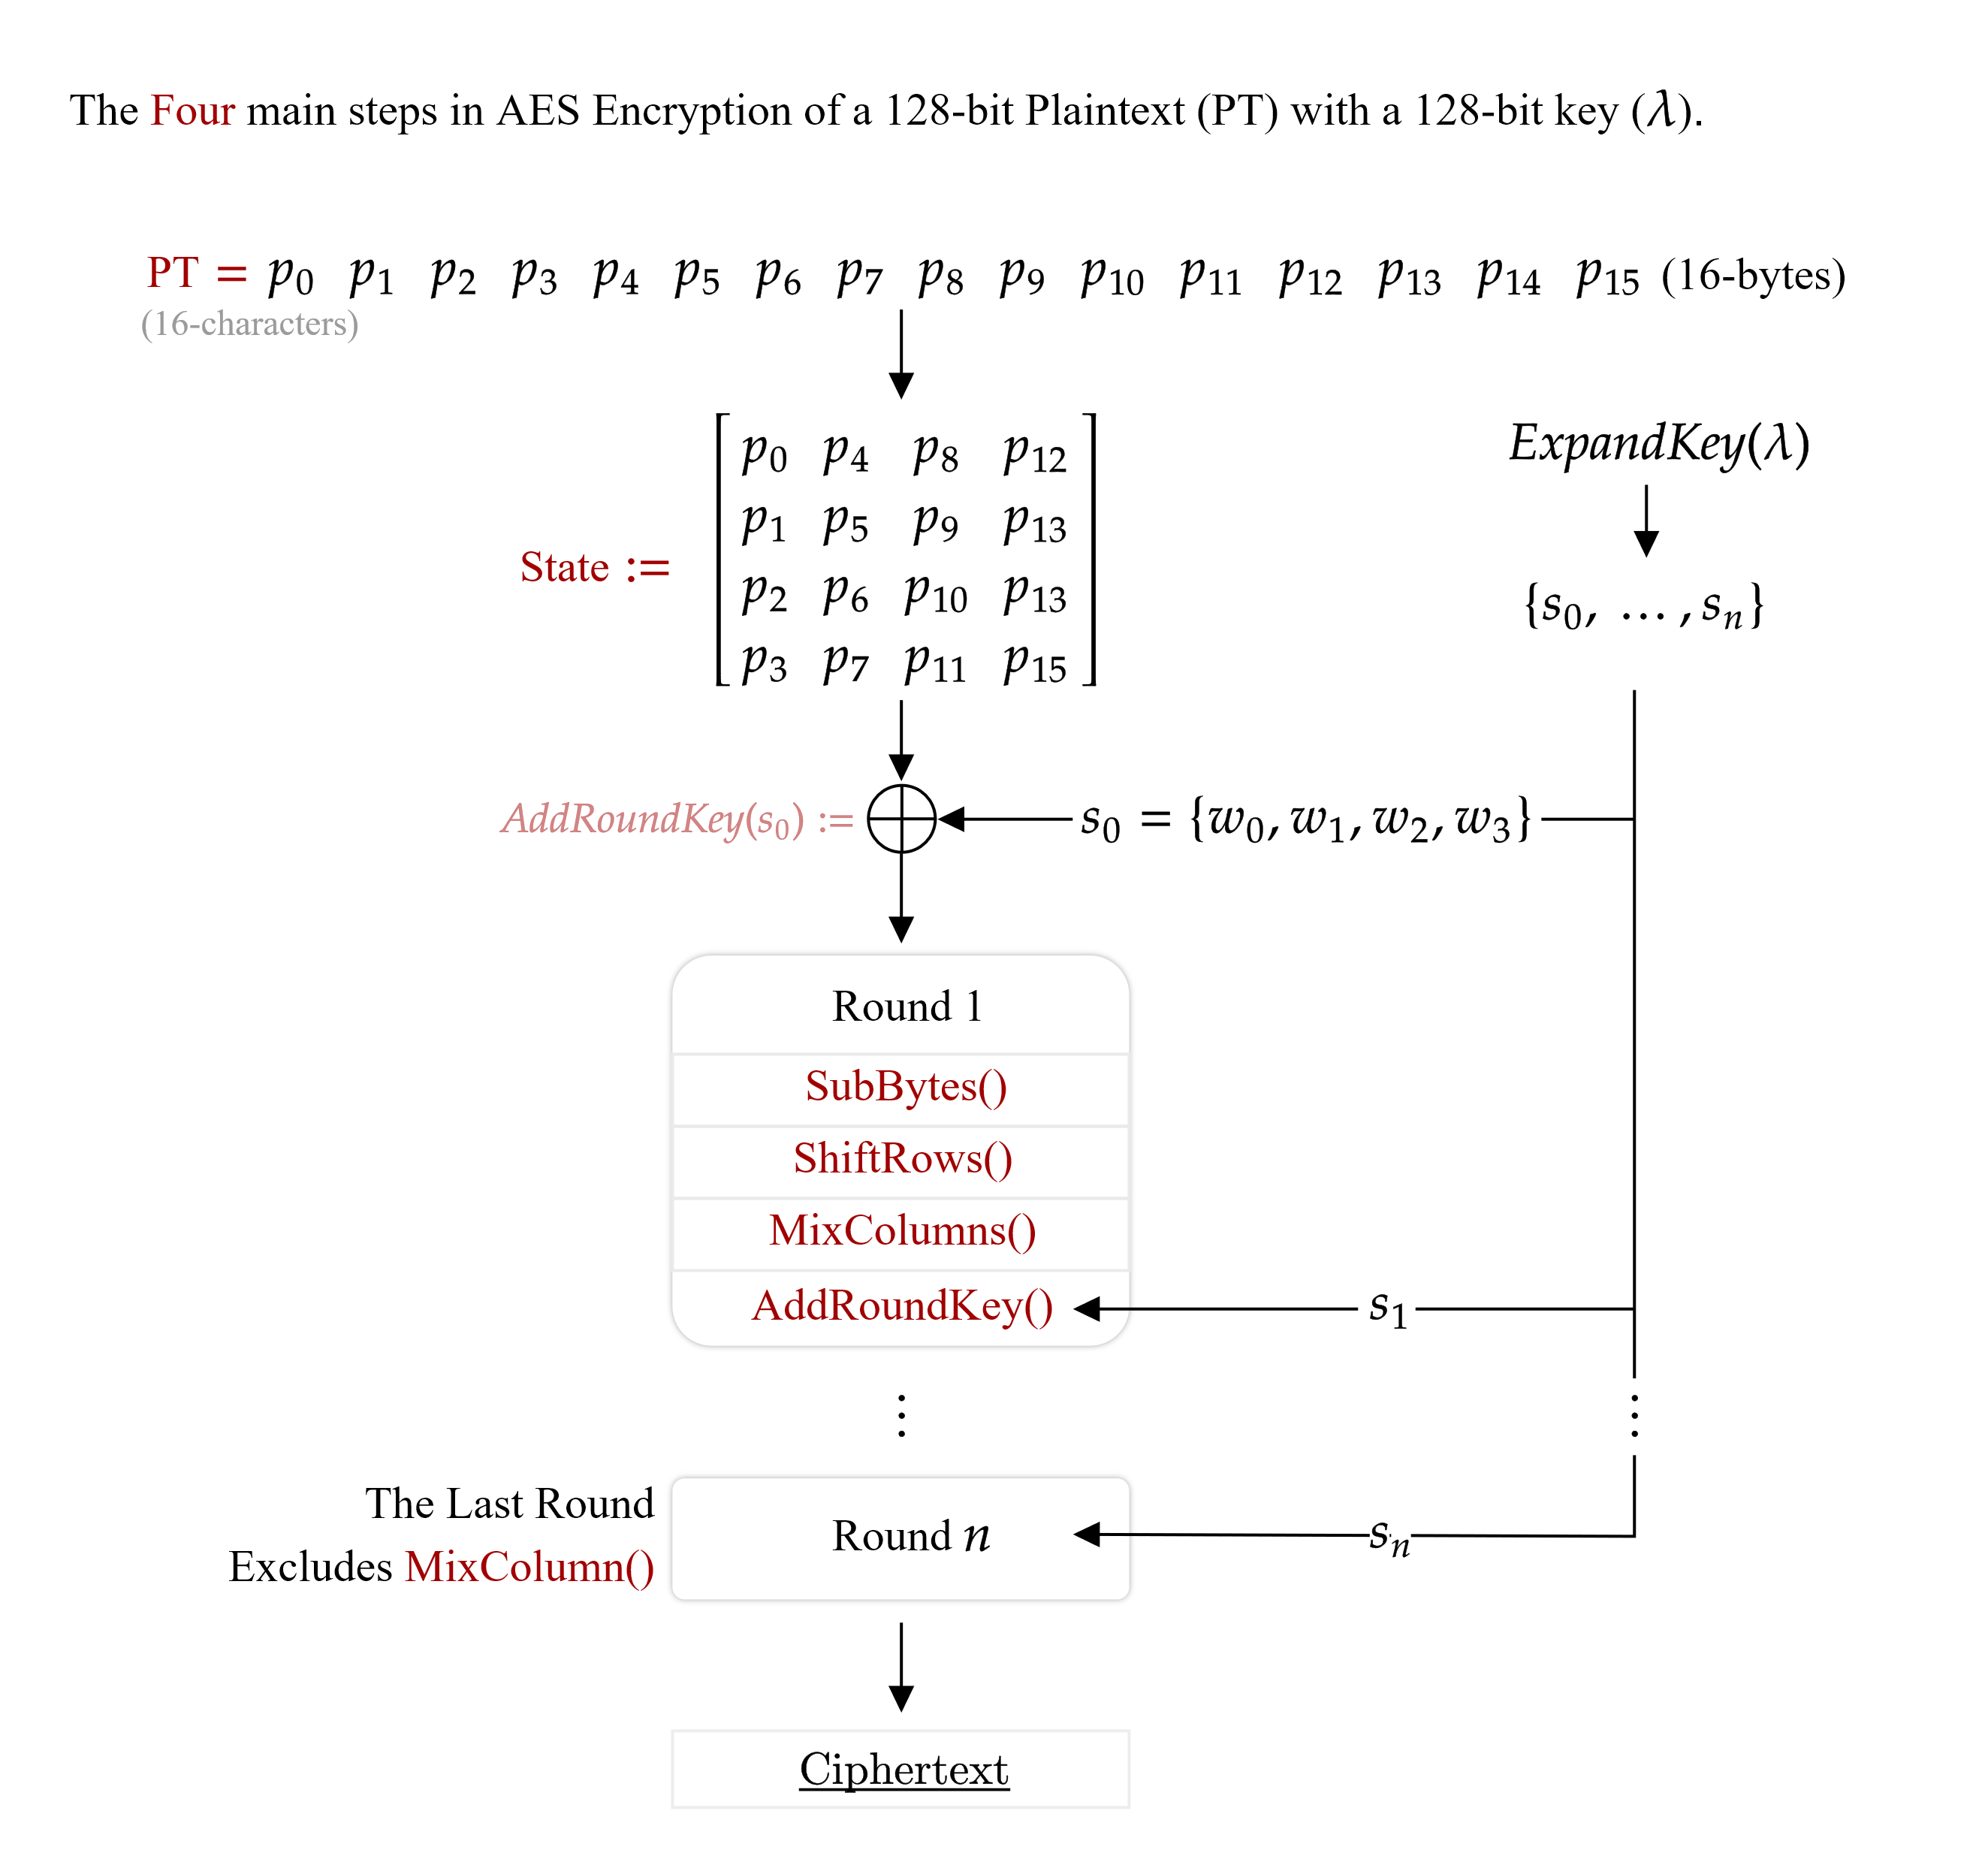
\includegraphics[width=1.1\textwidth]{Sections/sec/enc/aes/trans/high.png}

\vspace{2em}
\noindent
First the PT is transformed into a $4\times4$ matrix, called the \textbf{State}. The initial transformation is the \textbf{AddRoundKey} operation,
which XORs each column of the state with sub-key\\
$s_0=\{w_0,w_1,w_2,w_3\}$. I.e., $[p_0, p_1, p_2, p_3] \oplus [w_0]$ and so on. Recall $w_0=[b_0,b_1,b_2,b_3]$ 
for some byte $b_i$ of the initial key.
\newpage 

\noindent
To elaborate on the AddRoundKey operation:\\

\hspace{-3em}
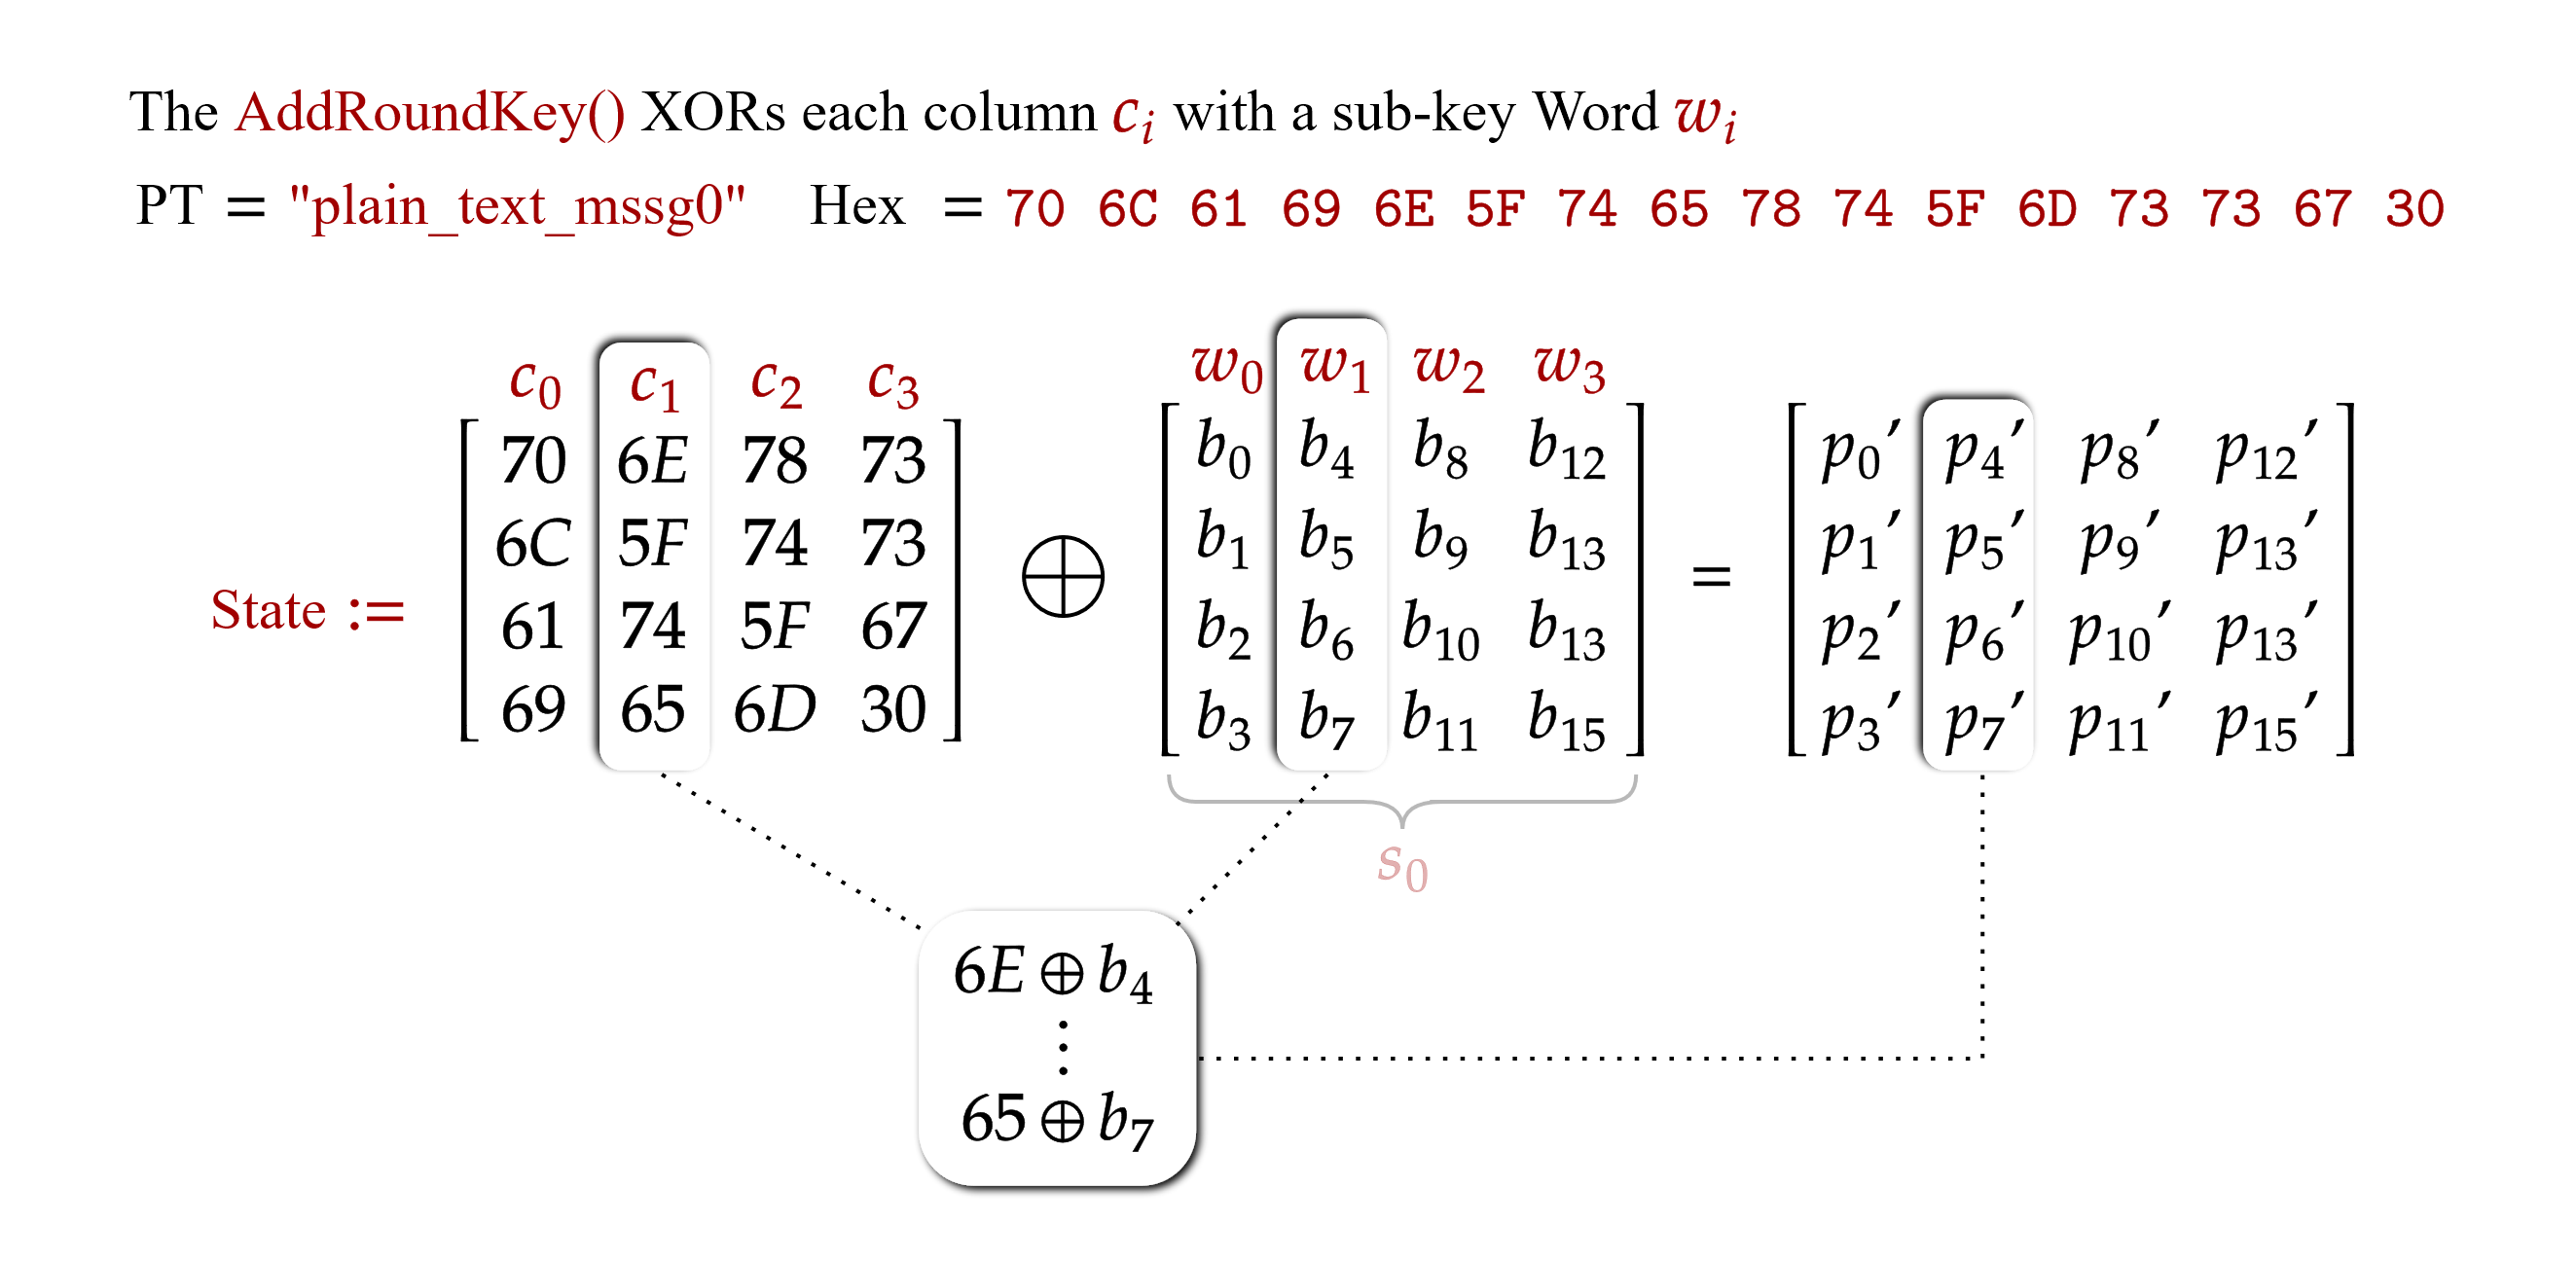
\includegraphics[width=1.1\textwidth]{Sections/sec/enc/aes/trans/add.png}
AddRoundKey takes a sub-key $s_i$ and XORs each Word $w_i$ with the corresponding column $c_i$ of the State.
\vspace{5em}

\hspace{-3em}
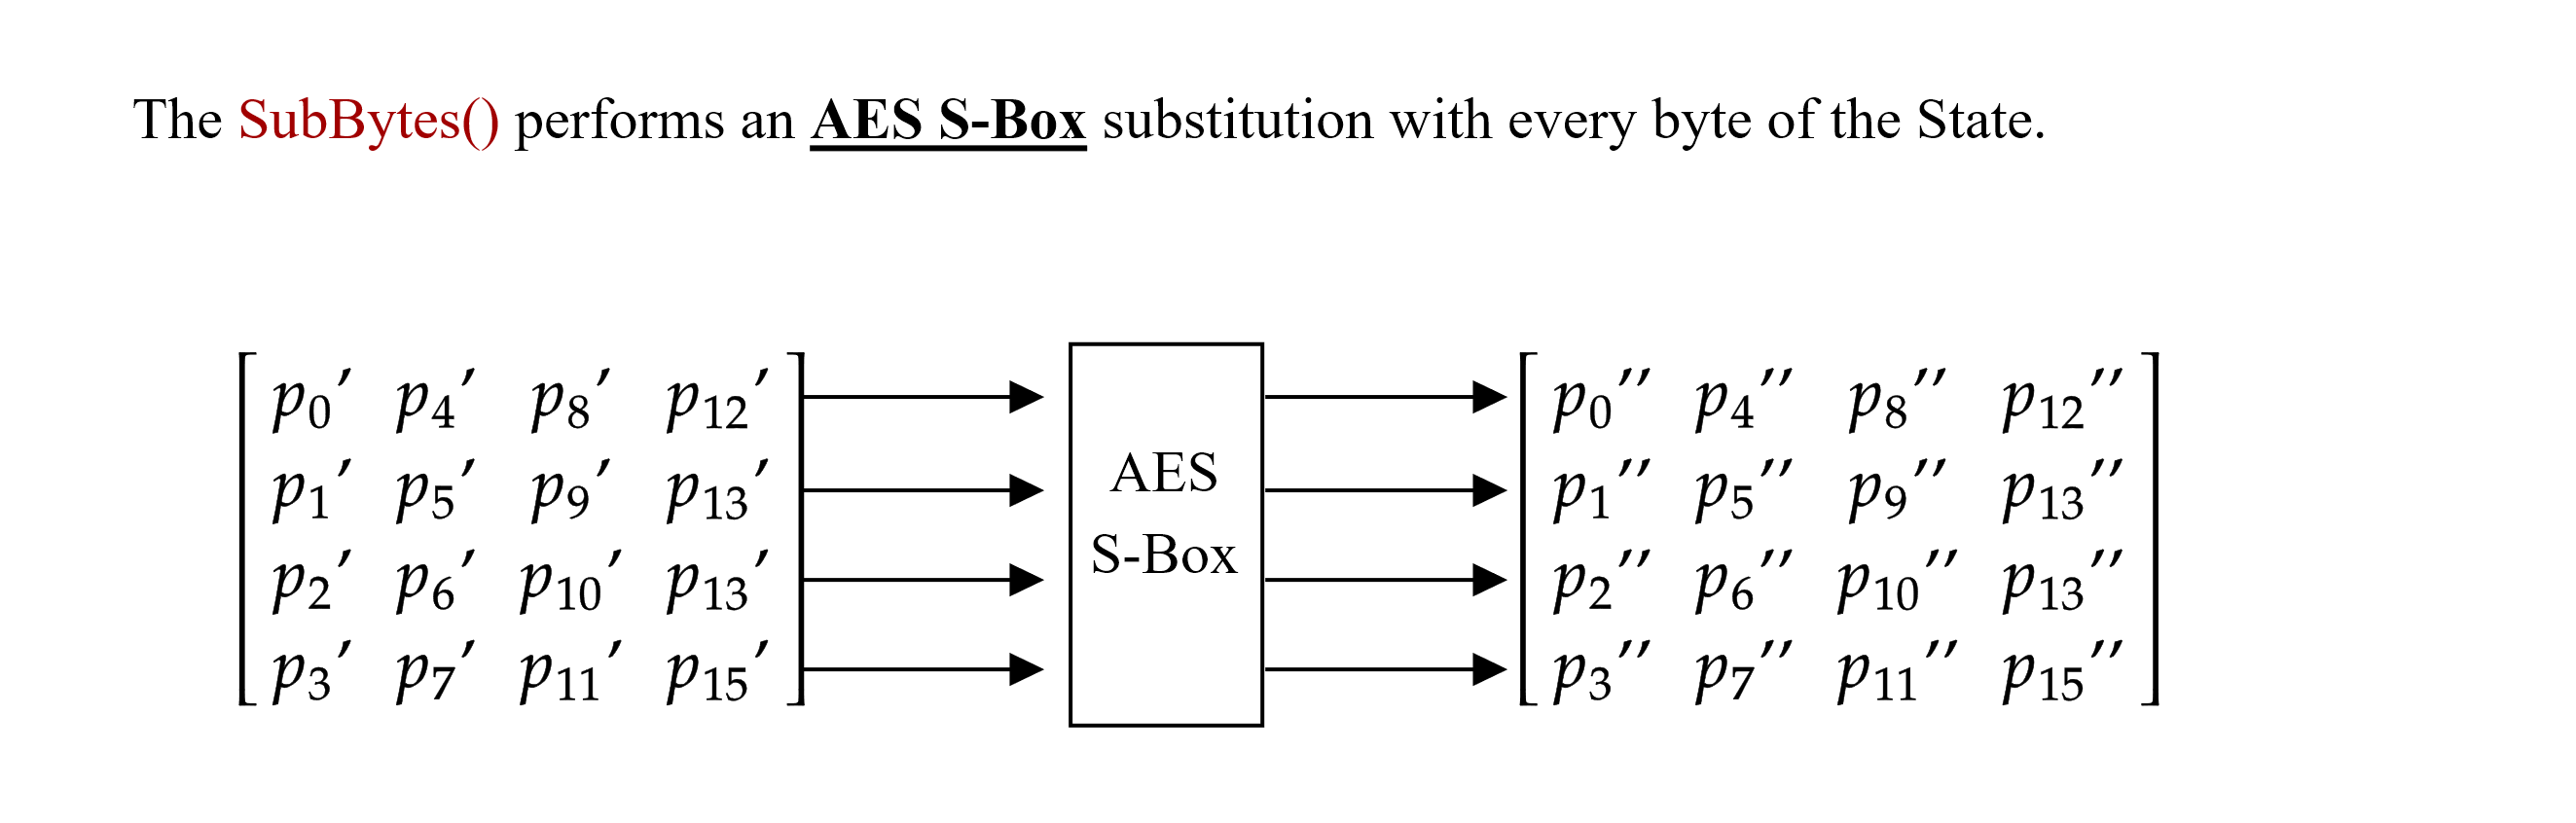
\includegraphics[width=1.1\textwidth]{Sections/sec/enc/aes/trans/sub.png}

\noindent
Just like in Key Expansion's (\ref{theo:key_expansion}) use of the S-Box on the last word of each sub-key. The PT undergoes 
a full substitution with the S-Box.

\newpage 

\hspace{-3em}
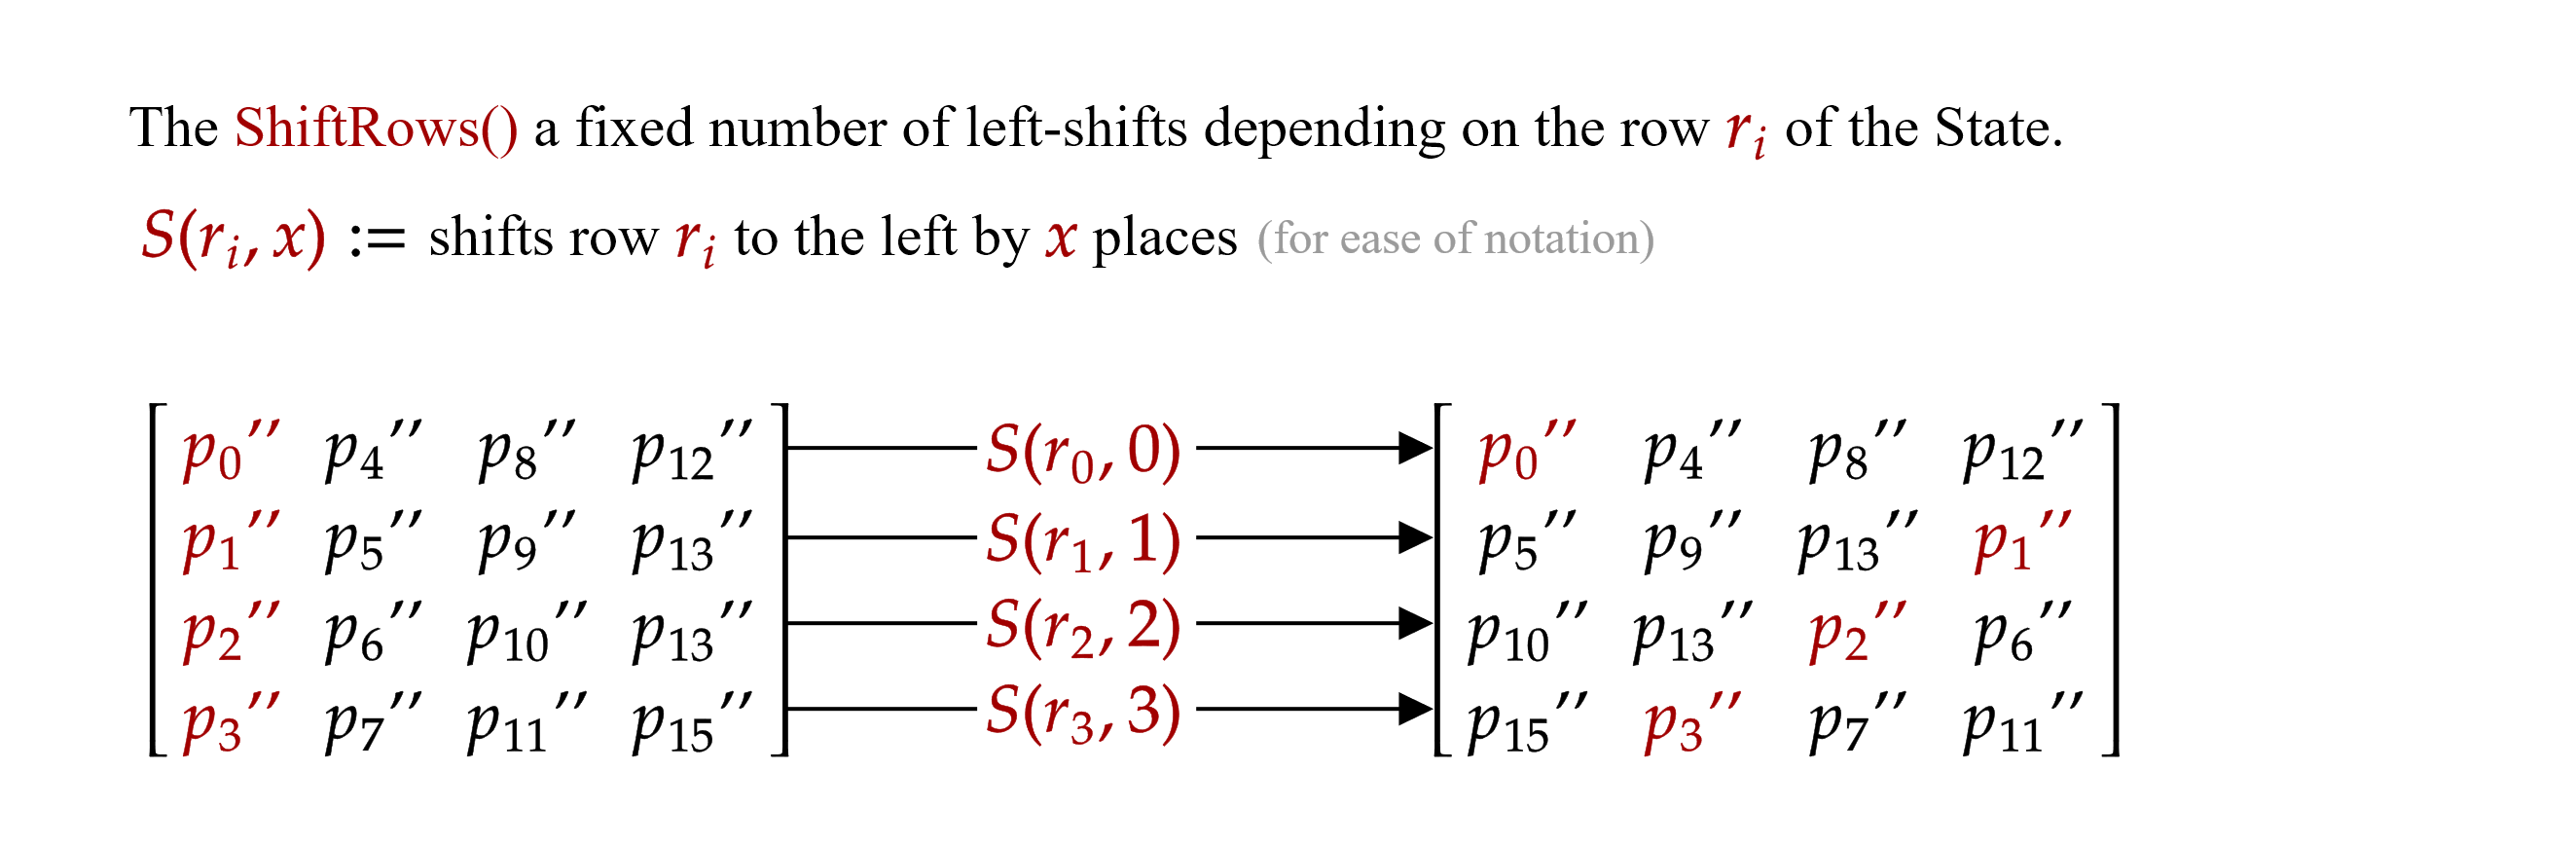
\includegraphics[width=1.1\textwidth]{Sections/sec/enc/aes/trans/shift.png}
\vspace{-1em}


\noindent
\underline{Below, the notation $\{01\}$ refers to a hex value.}\\

\vspace{-1em}
\hspace{-3em}
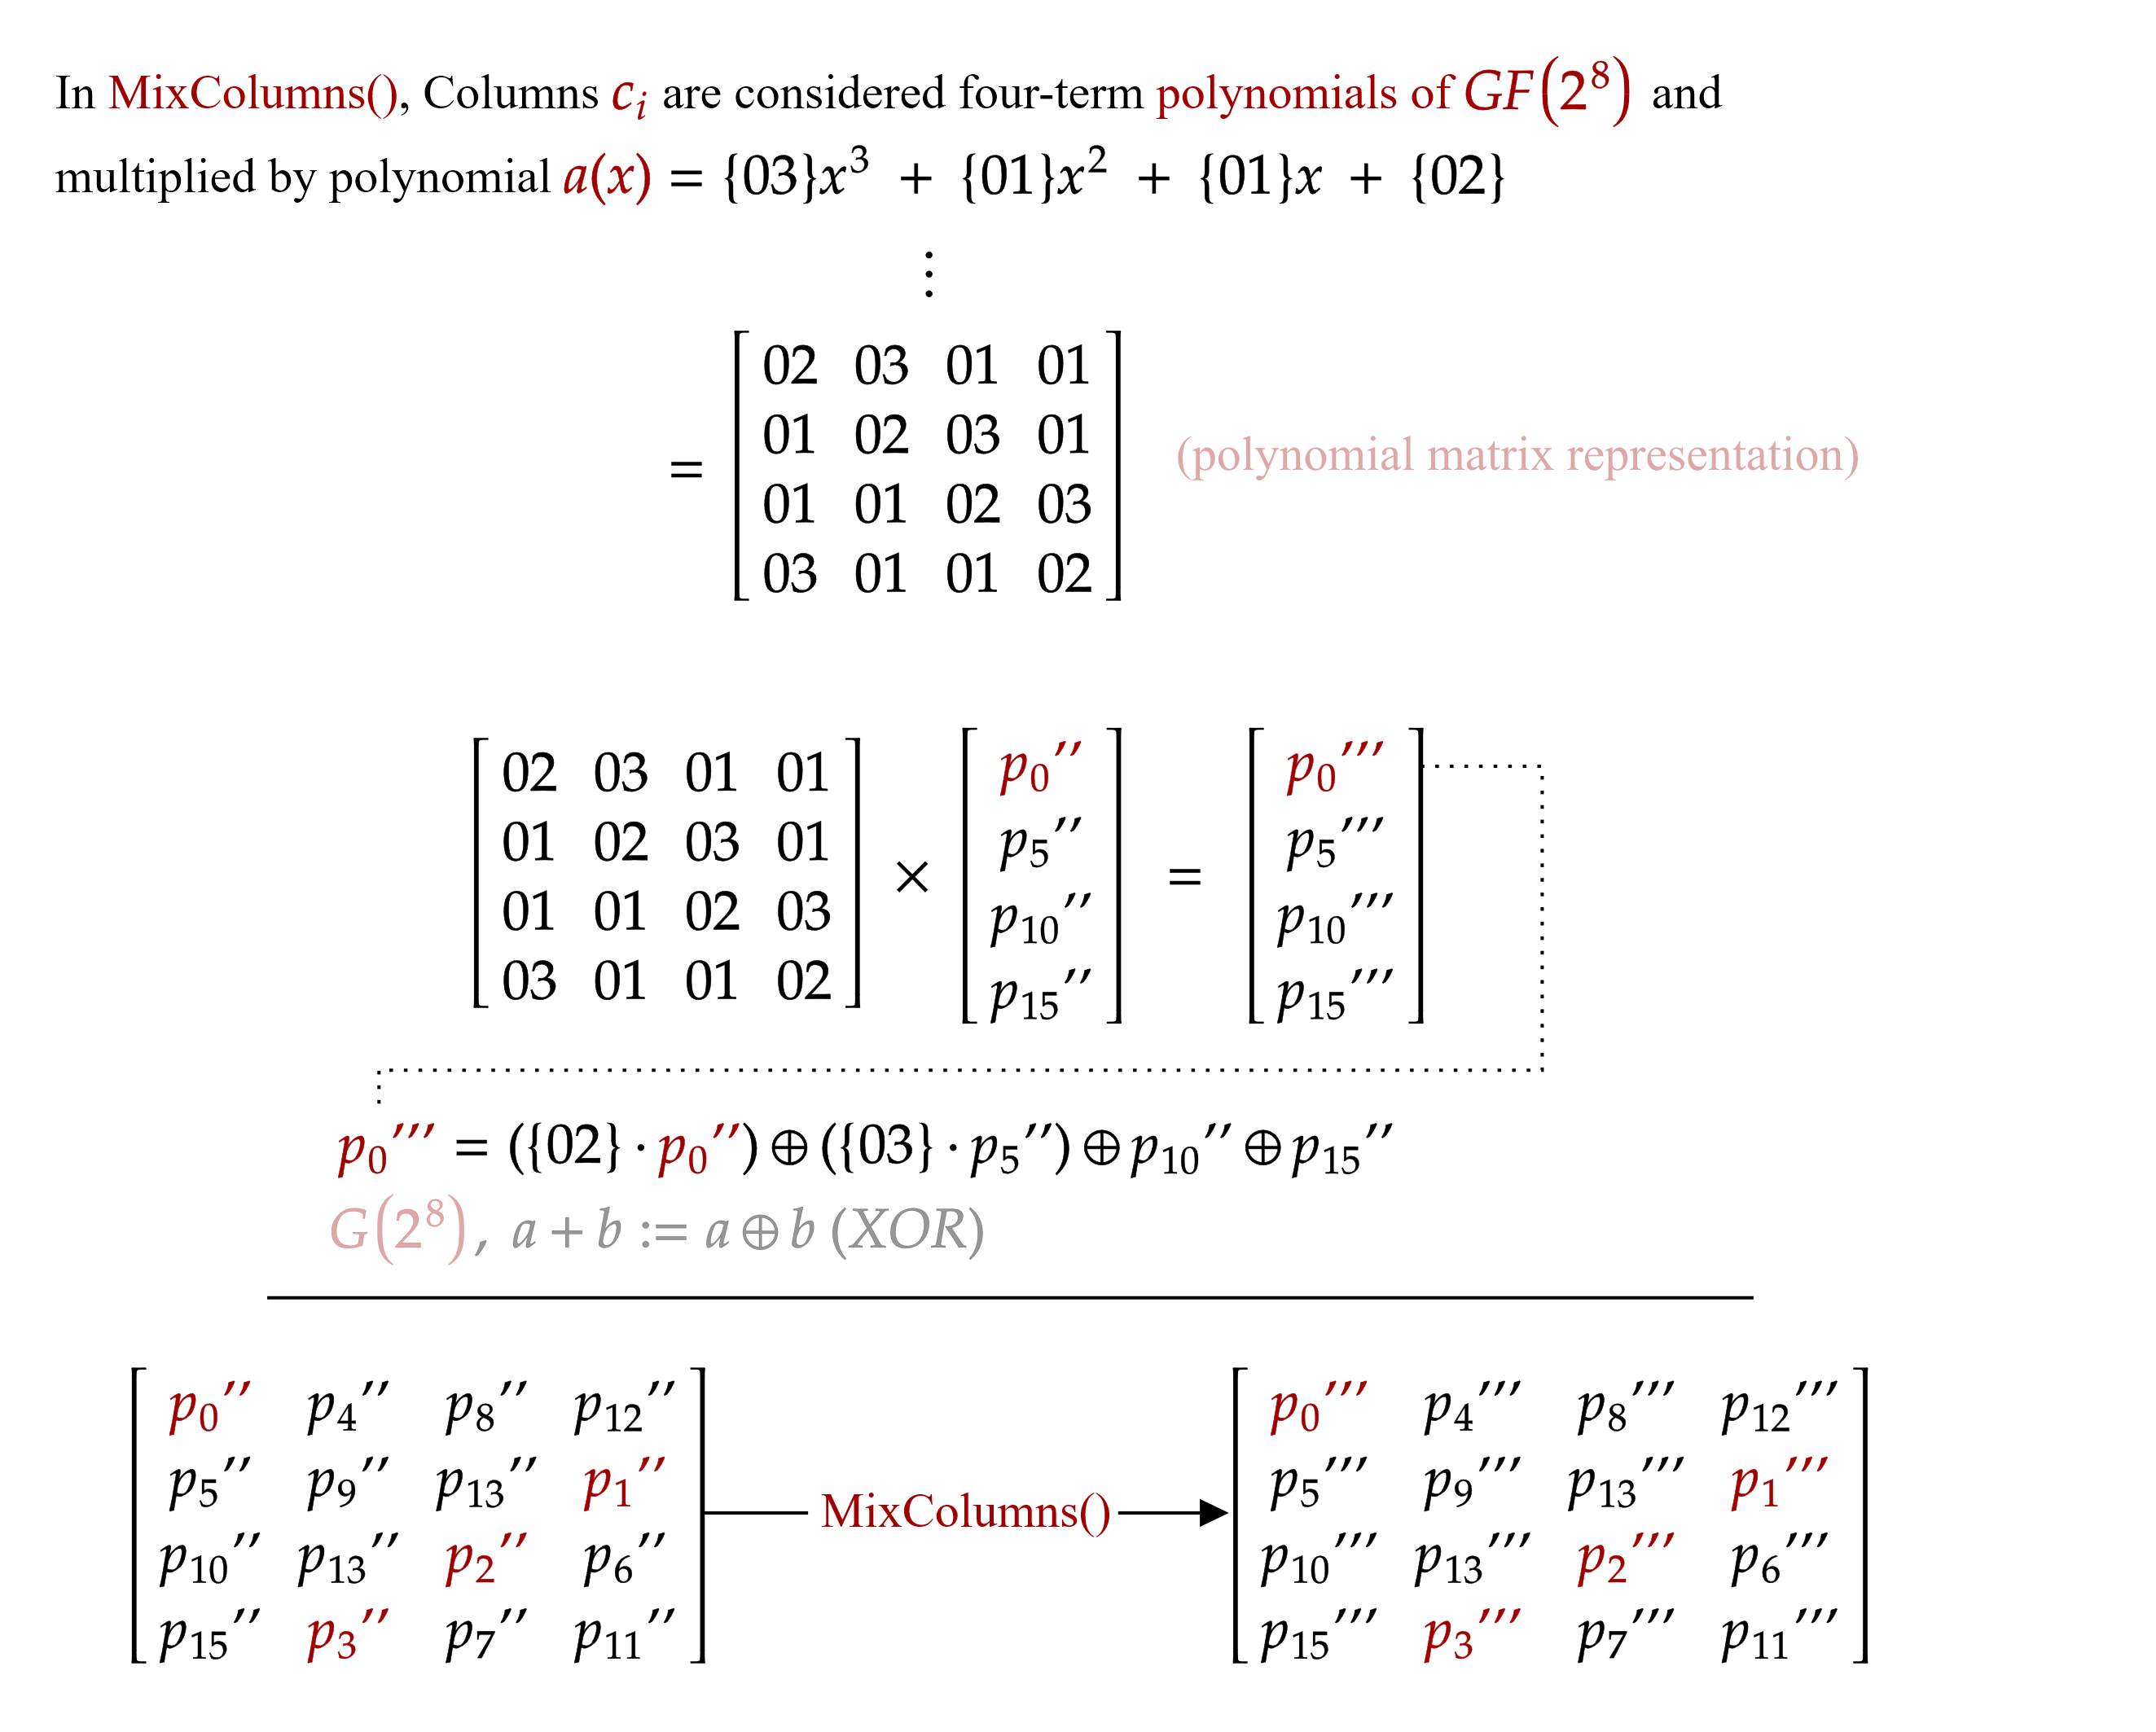
\includegraphics[width=1.1\textwidth]{Sections/sec/enc/aes/trans/mix.png}

\newpage

\noindent
This is the AES Encryption \& Decryption.

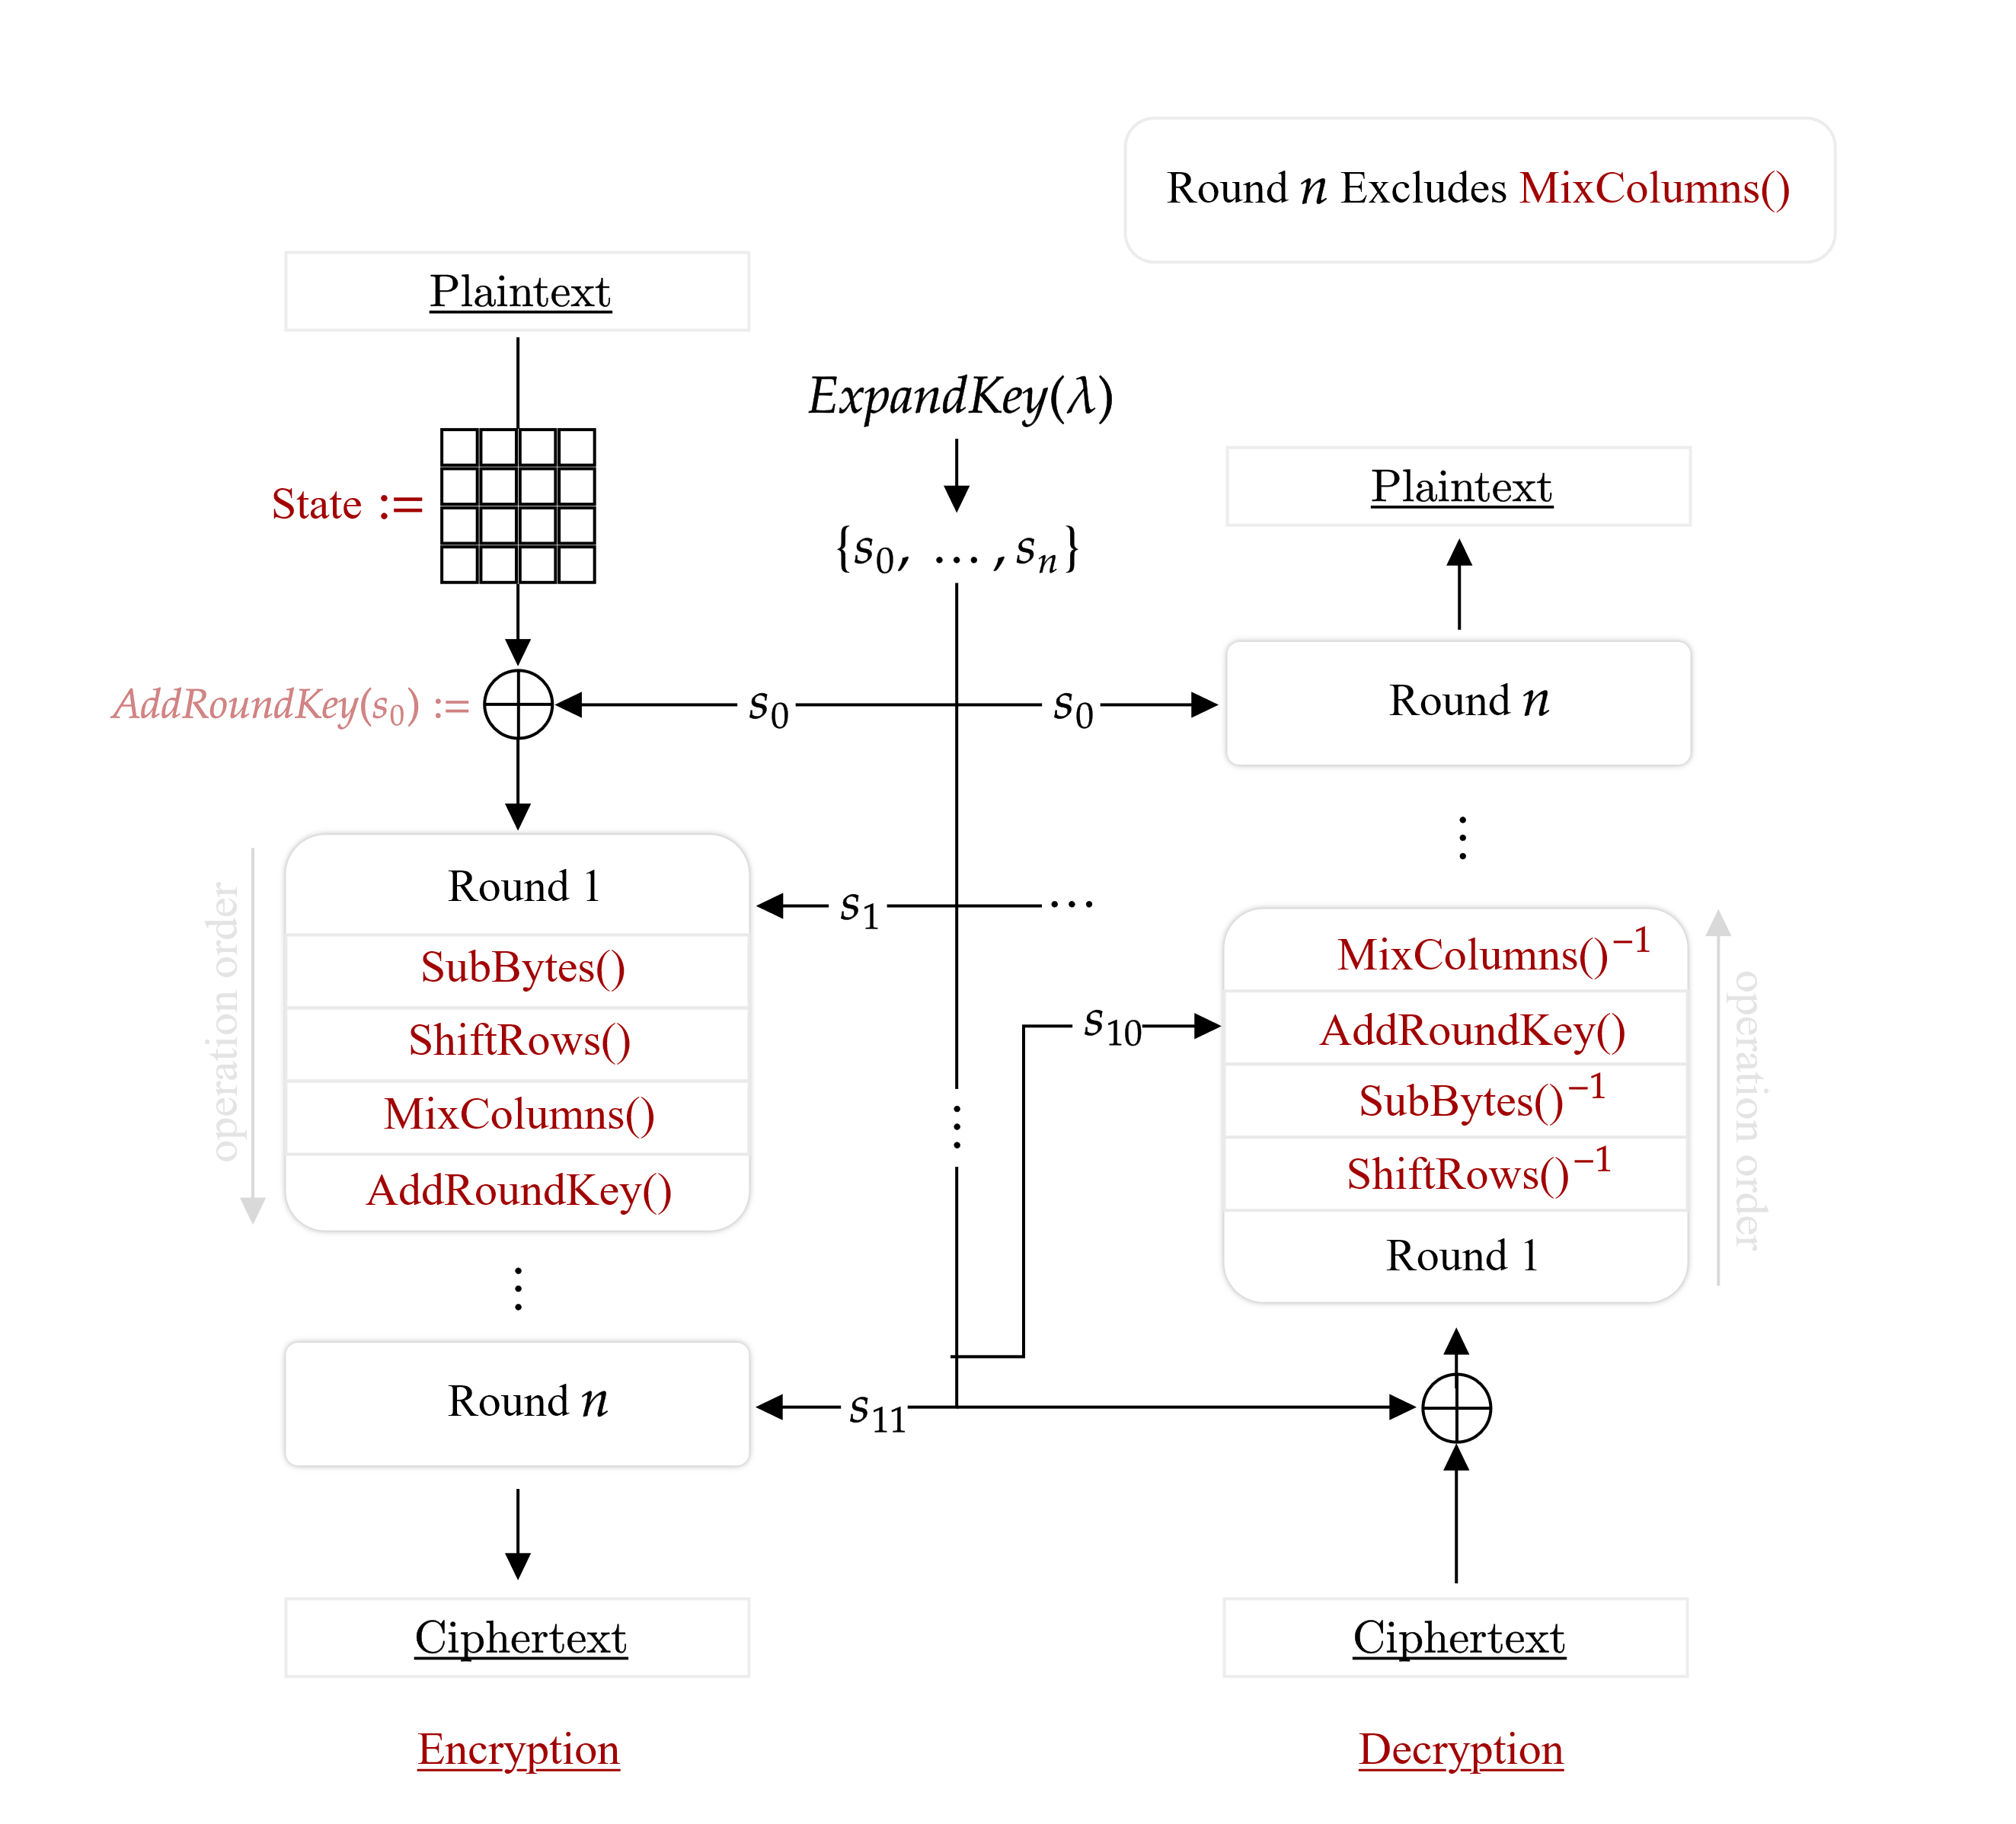
\includegraphics[width=1.1\textwidth]{Sections/sec/enc/aes/trans/ende.png}

\vspace{1em}
\noindent
For Decryption, the last scheduled key for Encryption is used as the initial transformation. Note the inverse 
operations of Decryption follow a different order than Encryption. This covers the basics of AES.



\bibliographystyle{plain} % We choose the "plain" reference style
\bibliography{refs} % Entries are in the refs.bib file



\end{document}
